% Options for packages loaded elsewhere
\PassOptionsToPackage{unicode}{hyperref}
\PassOptionsToPackage{hyphens}{url}
\PassOptionsToPackage{dvipsnames,svgnames,x11names}{xcolor}
%
\documentclass[
  letterpaper,
  DIV=11,
  numbers=noendperiod]{scrartcl}

\usepackage{amsmath,amssymb}
\usepackage{iftex}
\ifPDFTeX
  \usepackage[T1]{fontenc}
  \usepackage[utf8]{inputenc}
  \usepackage{textcomp} % provide euro and other symbols
\else % if luatex or xetex
  \usepackage{unicode-math}
  \defaultfontfeatures{Scale=MatchLowercase}
  \defaultfontfeatures[\rmfamily]{Ligatures=TeX,Scale=1}
\fi
\usepackage{lmodern}
\ifPDFTeX\else  
    % xetex/luatex font selection
\fi
% Use upquote if available, for straight quotes in verbatim environments
\IfFileExists{upquote.sty}{\usepackage{upquote}}{}
\IfFileExists{microtype.sty}{% use microtype if available
  \usepackage[]{microtype}
  \UseMicrotypeSet[protrusion]{basicmath} % disable protrusion for tt fonts
}{}
\makeatletter
\@ifundefined{KOMAClassName}{% if non-KOMA class
  \IfFileExists{parskip.sty}{%
    \usepackage{parskip}
  }{% else
    \setlength{\parindent}{0pt}
    \setlength{\parskip}{6pt plus 2pt minus 1pt}}
}{% if KOMA class
  \KOMAoptions{parskip=half}}
\makeatother
\usepackage{xcolor}
\setlength{\emergencystretch}{3em} % prevent overfull lines
\setcounter{secnumdepth}{-\maxdimen} % remove section numbering
% Make \paragraph and \subparagraph free-standing
\ifx\paragraph\undefined\else
  \let\oldparagraph\paragraph
  \renewcommand{\paragraph}[1]{\oldparagraph{#1}\mbox{}}
\fi
\ifx\subparagraph\undefined\else
  \let\oldsubparagraph\subparagraph
  \renewcommand{\subparagraph}[1]{\oldsubparagraph{#1}\mbox{}}
\fi


\providecommand{\tightlist}{%
  \setlength{\itemsep}{0pt}\setlength{\parskip}{0pt}}\usepackage{longtable,booktabs,array}
\usepackage{calc} % for calculating minipage widths
% Correct order of tables after \paragraph or \subparagraph
\usepackage{etoolbox}
\makeatletter
\patchcmd\longtable{\par}{\if@noskipsec\mbox{}\fi\par}{}{}
\makeatother
% Allow footnotes in longtable head/foot
\IfFileExists{footnotehyper.sty}{\usepackage{footnotehyper}}{\usepackage{footnote}}
\makesavenoteenv{longtable}
\usepackage{graphicx}
\makeatletter
\def\maxwidth{\ifdim\Gin@nat@width>\linewidth\linewidth\else\Gin@nat@width\fi}
\def\maxheight{\ifdim\Gin@nat@height>\textheight\textheight\else\Gin@nat@height\fi}
\makeatother
% Scale images if necessary, so that they will not overflow the page
% margins by default, and it is still possible to overwrite the defaults
% using explicit options in \includegraphics[width, height, ...]{}
\setkeys{Gin}{width=\maxwidth,height=\maxheight,keepaspectratio}
% Set default figure placement to htbp
\makeatletter
\def\fps@figure{htbp}
\makeatother

\KOMAoption{captions}{tableheading}
\makeatletter
\makeatother
\makeatletter
\makeatother
\makeatletter
\@ifpackageloaded{caption}{}{\usepackage{caption}}
\AtBeginDocument{%
\ifdefined\contentsname
  \renewcommand*\contentsname{Table of contents}
\else
  \newcommand\contentsname{Table of contents}
\fi
\ifdefined\listfigurename
  \renewcommand*\listfigurename{List of Figures}
\else
  \newcommand\listfigurename{List of Figures}
\fi
\ifdefined\listtablename
  \renewcommand*\listtablename{List of Tables}
\else
  \newcommand\listtablename{List of Tables}
\fi
\ifdefined\figurename
  \renewcommand*\figurename{Figure}
\else
  \newcommand\figurename{Figure}
\fi
\ifdefined\tablename
  \renewcommand*\tablename{Table}
\else
  \newcommand\tablename{Table}
\fi
}
\@ifpackageloaded{float}{}{\usepackage{float}}
\floatstyle{ruled}
\@ifundefined{c@chapter}{\newfloat{codelisting}{h}{lop}}{\newfloat{codelisting}{h}{lop}[chapter]}
\floatname{codelisting}{Listing}
\newcommand*\listoflistings{\listof{codelisting}{List of Listings}}
\makeatother
\makeatletter
\@ifpackageloaded{caption}{}{\usepackage{caption}}
\@ifpackageloaded{subcaption}{}{\usepackage{subcaption}}
\makeatother
\makeatletter
\@ifpackageloaded{tcolorbox}{}{\usepackage[skins,breakable]{tcolorbox}}
\makeatother
\makeatletter
\@ifundefined{shadecolor}{\definecolor{shadecolor}{rgb}{.97, .97, .97}}
\makeatother
\makeatletter
\makeatother
\makeatletter
\makeatother
\ifLuaTeX
  \usepackage{selnolig}  % disable illegal ligatures
\fi
\IfFileExists{bookmark.sty}{\usepackage{bookmark}}{\usepackage{hyperref}}
\IfFileExists{xurl.sty}{\usepackage{xurl}}{} % add URL line breaks if available
\urlstyle{same} % disable monospaced font for URLs
\hypersetup{
  colorlinks=true,
  linkcolor={blue},
  filecolor={Maroon},
  citecolor={Blue},
  urlcolor={Blue},
  pdfcreator={LaTeX via pandoc}}

\author{}
\date{}

\begin{document}
\ifdefined\Shaded\renewenvironment{Shaded}{\begin{tcolorbox}[borderline west={3pt}{0pt}{shadecolor}, boxrule=0pt, breakable, enhanced, frame hidden, sharp corners, interior hidden]}{\end{tcolorbox}}\fi

\hypertarget{title-little-kids-big-adventures-hiking-with-kids-around-knoxville-tn}{%
\section{Title: Little Kids, Big Adventures: Hiking with Kids Around
Knoxville,
TN}\label{title-little-kids-big-adventures-hiking-with-kids-around-knoxville-tn}}

Little Kids, Big Adventures: A Guide to Family Hikes Around Knoxville

Katie Rosenberg and Joshua Rosenberg To be published by UT Press
(anticipated 2026)

\newpage{}

\hypertarget{preface-a-story-about-a-hike}{%
\subsection{Preface: A Story About a
Hike}\label{preface-a-story-about-a-hike}}

\hypertarget{a-story-about-a-hike}{%
\subsubsection{A Story About a Hike}\label{a-story-about-a-hike}}

First comes the vision. A beautiful sunny day out in nature with your
family. Your young children happily throwing rocks in rivers, wading in
creeks. Oh, look! Little JoJo caught a crawdad! A picnic where everyone
enjoys the food and nobody complains because you made the peanut butter
and jelly on the dark brown bread (otherwise known as wheat). You cover
extensive ground! Your children bask in nature! You get gorgeous
pictures to share on social media. Then, the kiddos nap peacefully on
the ride home while you and your spouse agree on what music or podcast
to listen to.

\emph{Record Scratch}

Sure, we'd all love for the above vision to be reality, but the truth is
a bit messier, potentially whinier (which comes with the territory when
doing activities with young kids), and comes with unexpected bumps in
the road (also known as surprises, depending on how you look at these
kinds of things).

In reality, you might be ready to throw in the towel before you even
leave your house. Packing for a day hike seems like it should be simple,
but by the time you consider what your family will need and plan
properly for the trail you'll be spending time on, you've already
expended a lot of mental energy and can't muster up the patience for the
car ride to the trailhead.

Once you arrive, the kids are hungry for the forty-third time, the baby
falls and scrapes her knee and refuses to go in the carrier pack, and
your oldest can't be pulled away from the creek just beyond the
trailhead to even start the hike.

We've been there more times than we can count, and have felt more relief
in a hike being over than we felt excitement to go on the hike in the
first place. However, we've also grown as a family who hikes, honed in
on the process, adjusted our expectations, and have built some beautiful
memories in the process.

If you're a family who enjoys the outdoors, wants to enjoy the outdoors,
and wants to learn more about the family hike adventures that await you,
this guide is for you. In this guide, we'll provide hiking and gear
recommendations, all designed with young families in mind.

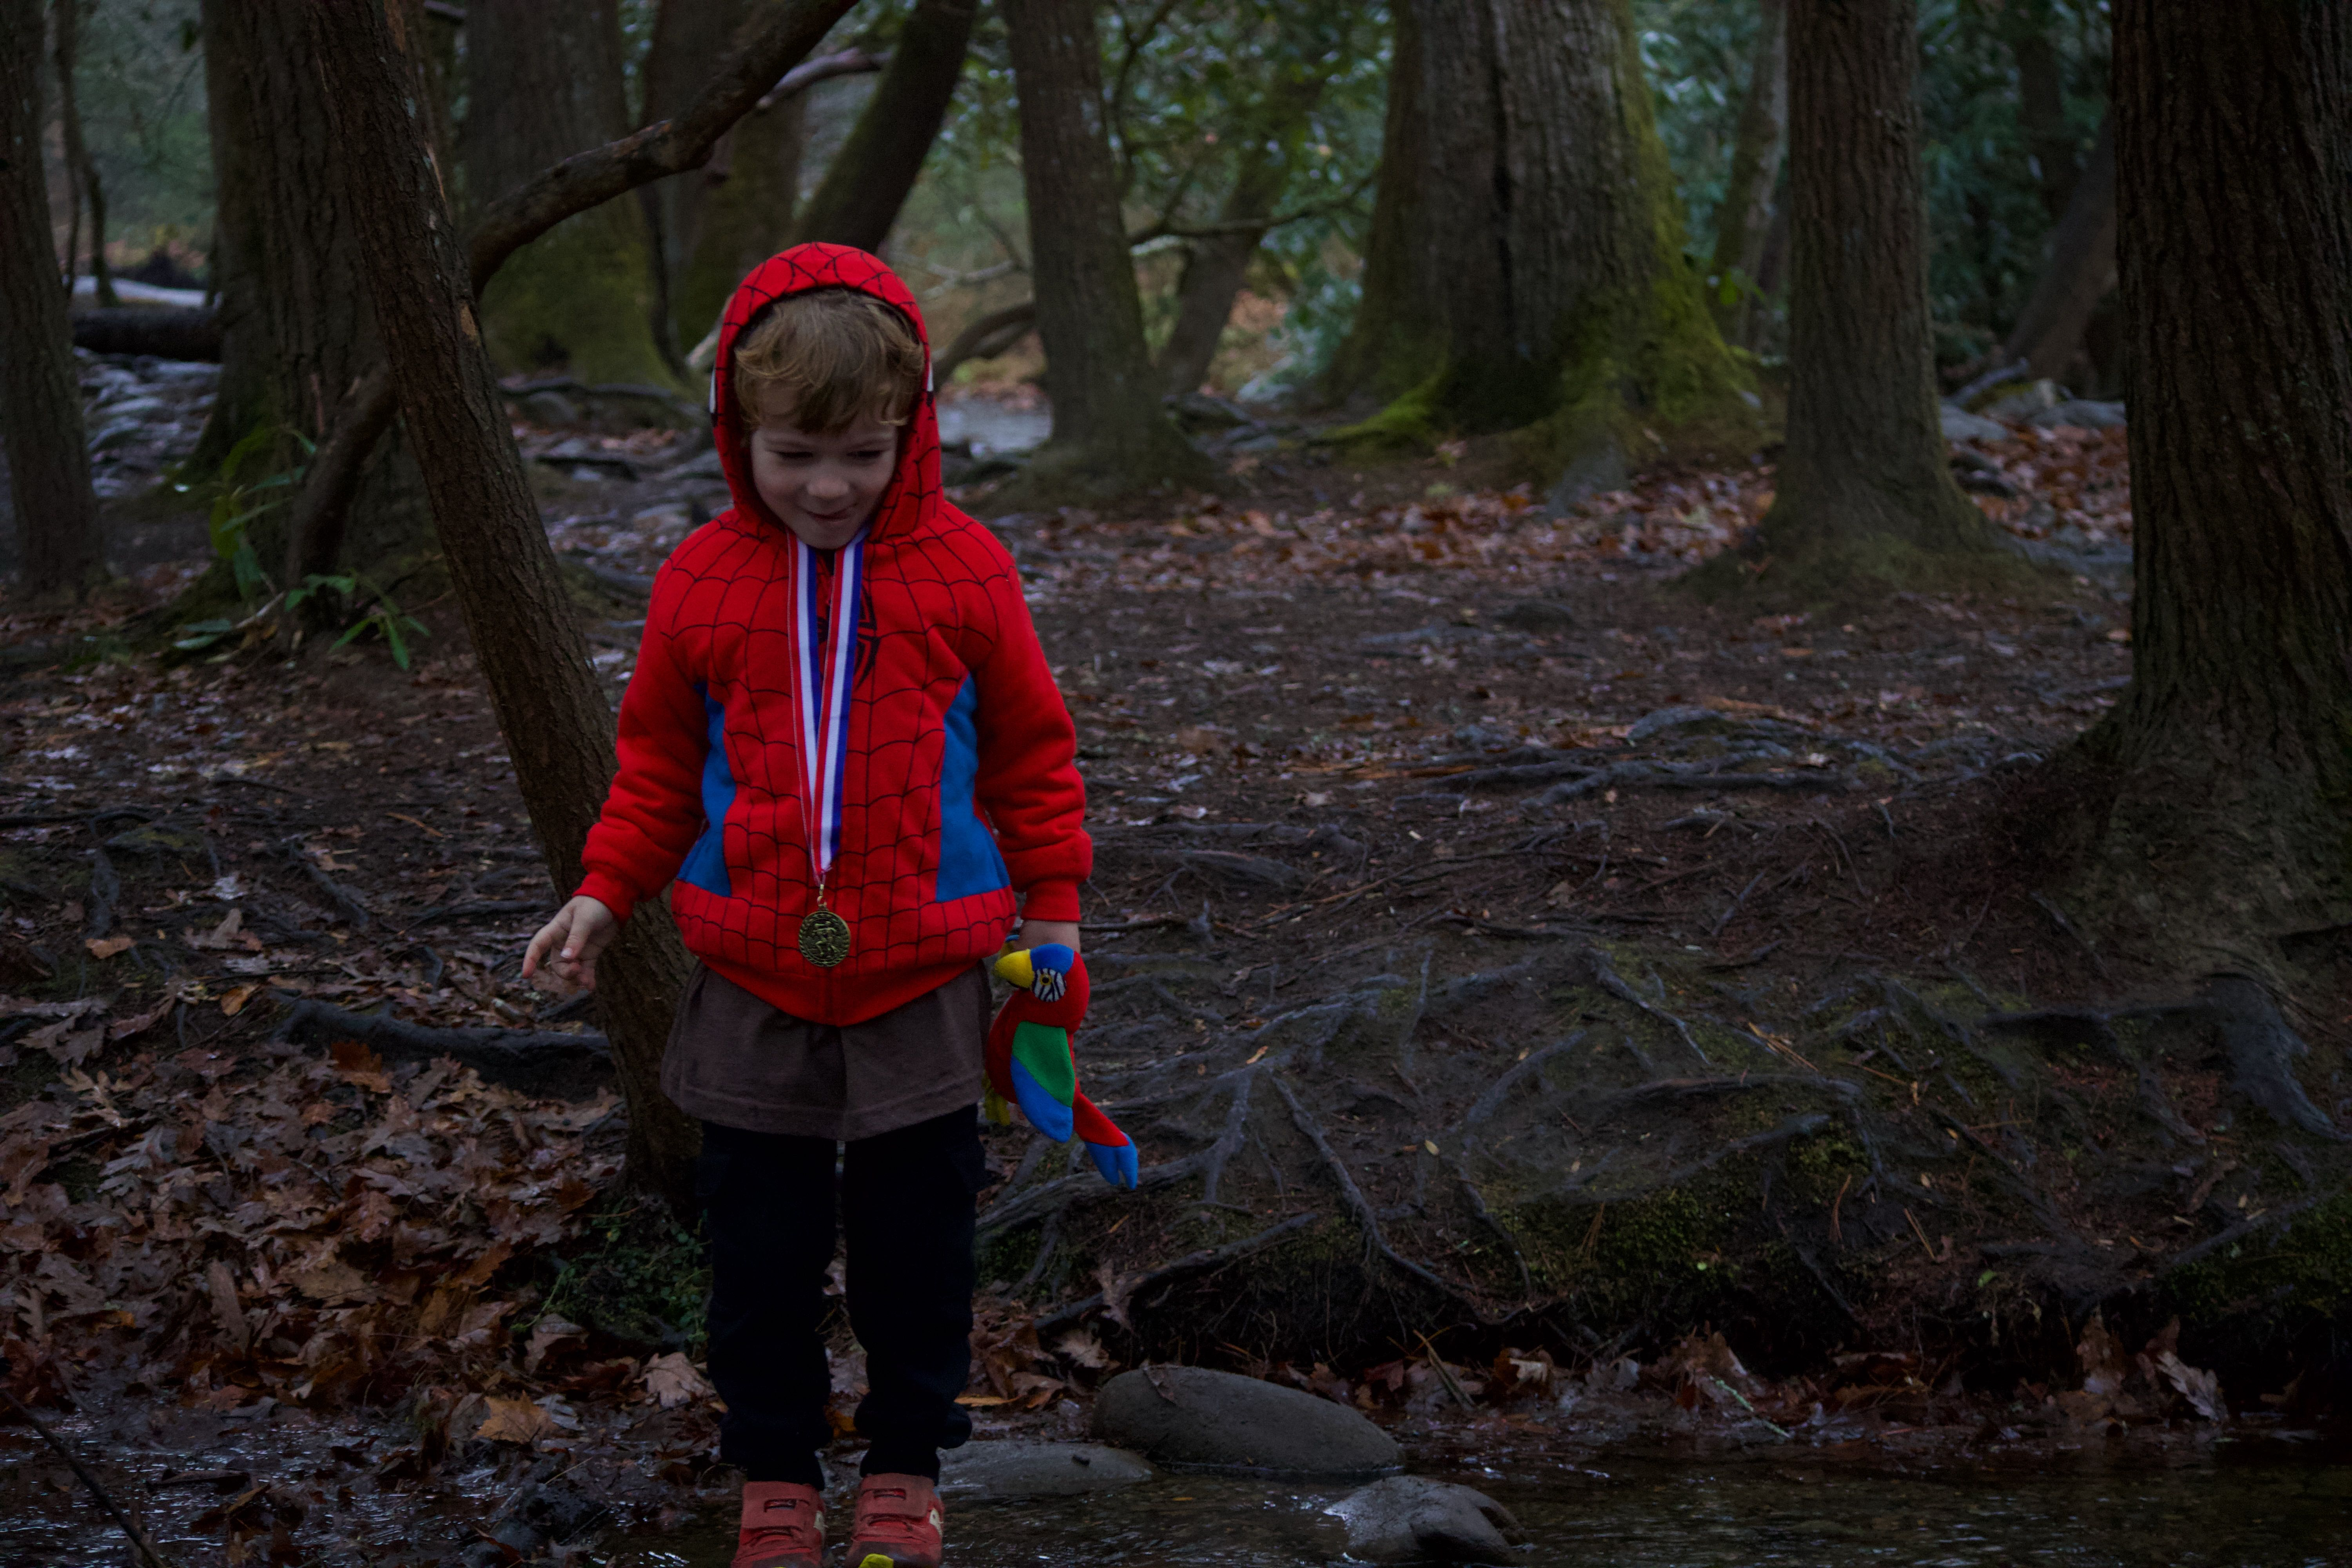
\includegraphics{img/jonahinthewater.jpg}

\hypertarget{what-this-book-is-about-and-why-we-wrote-it}{%
\subsubsection{What this Book is About (and Why We Wrote
It)}\label{what-this-book-is-about-and-why-we-wrote-it}}

Xx

\hypertarget{who-this-book-is-for}{%
\subsubsection{Who this Book is For}\label{who-this-book-is-for}}

Xx

\hypertarget{where-the-hikes-are}{%
\subsubsection{Where the Hikes Are}\label{where-the-hikes-are}}

Xx

\hypertarget{when-to-go}{%
\subsubsection{When to Go?}\label{when-to-go}}

Xx

See you on the trail!

\newpage{}

\hypertarget{finding-a-hike}{%
\subsection{Finding a Hike}\label{finding-a-hike}}

What's the best hike?

What's the best hike for families? - Avoiding bucket list traveling (but
still featuring some epic spots!) - Too many people visiting the busy,
crowded places

Age Ranges - Infants: birth - toddler stages lwho are carried -
Toddlers: around one-two year-olds who can walk some of the trail (being
carried for other parts), or all of short trails. - Little kids: Two-
four or five years who can walk all of short trails, and even some parts
of lengthier trails. - Big kids: Four -eight or nine who can walk longer
distance are who up for bigger challenges - Pre-teens and older: Eight
or nine or up

Other Considerations -- accessible: To strollers and wheelchairs

\newpage{}

\hypertarget{top-5}{%
\subsection{Top 5}\label{top-5}}

\hypertarget{top-5---very-young-children}{%
\subsubsection{Top 5 - Very Young
Children}\label{top-5---very-young-children}}

\begin{enumerate}
\def\labelenumi{\arabic{enumi}.}
\tightlist
\item
  Xx
\item
  Xx
\item
  Xx
\item
  Xx
\item
  Xx
\end{enumerate}

\hypertarget{top-5---a-short-drive}{%
\subsubsection{Top 5 - A Short Drive}\label{top-5---a-short-drive}}

\begin{enumerate}
\def\labelenumi{\arabic{enumi}.}
\tightlist
\item
  Xx
\item
  Xx
\item
  Xx
\item
  Xx
\item
  Xx
\end{enumerate}

\hypertarget{top-5---most-beautiful}{%
\subsubsection{Top 5 - Most Beautiful}\label{top-5---most-beautiful}}

\begin{enumerate}
\def\labelenumi{\arabic{enumi}.}
\tightlist
\item
  Xx
\item
  Xx
\item
  Xx
\item
  Xx
\item
  Xx
\end{enumerate}

\hypertarget{top-5---adventures-for-older-kids}{%
\subsubsection{Top 5 - Adventures for Older
Kids}\label{top-5---adventures-for-older-kids}}

\begin{enumerate}
\def\labelenumi{\arabic{enumi}.}
\tightlist
\item
  Xx
\item
  Xx
\item
  Xx
\item
  Xx
\item
  Xx
\end{enumerate}

\hypertarget{top-5---must-do}{%
\subsubsection{Top 5 - Must-do!}\label{top-5---must-do}}

\begin{enumerate}
\def\labelenumi{\arabic{enumi}.}
\tightlist
\item
  Xx
\item
  Xx
\item
  Xx
\item
  Xx
\item
  Xx
\end{enumerate}

\hypertarget{considerations-for-your-first-hike}{%
\subsection{Considerations for Your First
Hike}\label{considerations-for-your-first-hike}}

You do not need much specialized gear to go on your first hike. Indeed,
select a particular hike at a particular time, and you will not need
anything particular at all. We detail those considerations: selecting a
particular hike at a particular time and a few other things that are
needed on practically every hike.

Define your own adventure. Do you need a hike that will help burn older
kids' energy? Or do you have toddlers who simply want to touch every
leaf and rock you pass? Decide what's most important for your family
hike and pick a trail that best supports that!

Give kids' time. Want to encourage your kids to love hiking and being
outside? Let them develop their own interests and explore their own
curiosities when you go on a hike. Sometimes this might mean playing in
a creek for half of your planned hiking time.

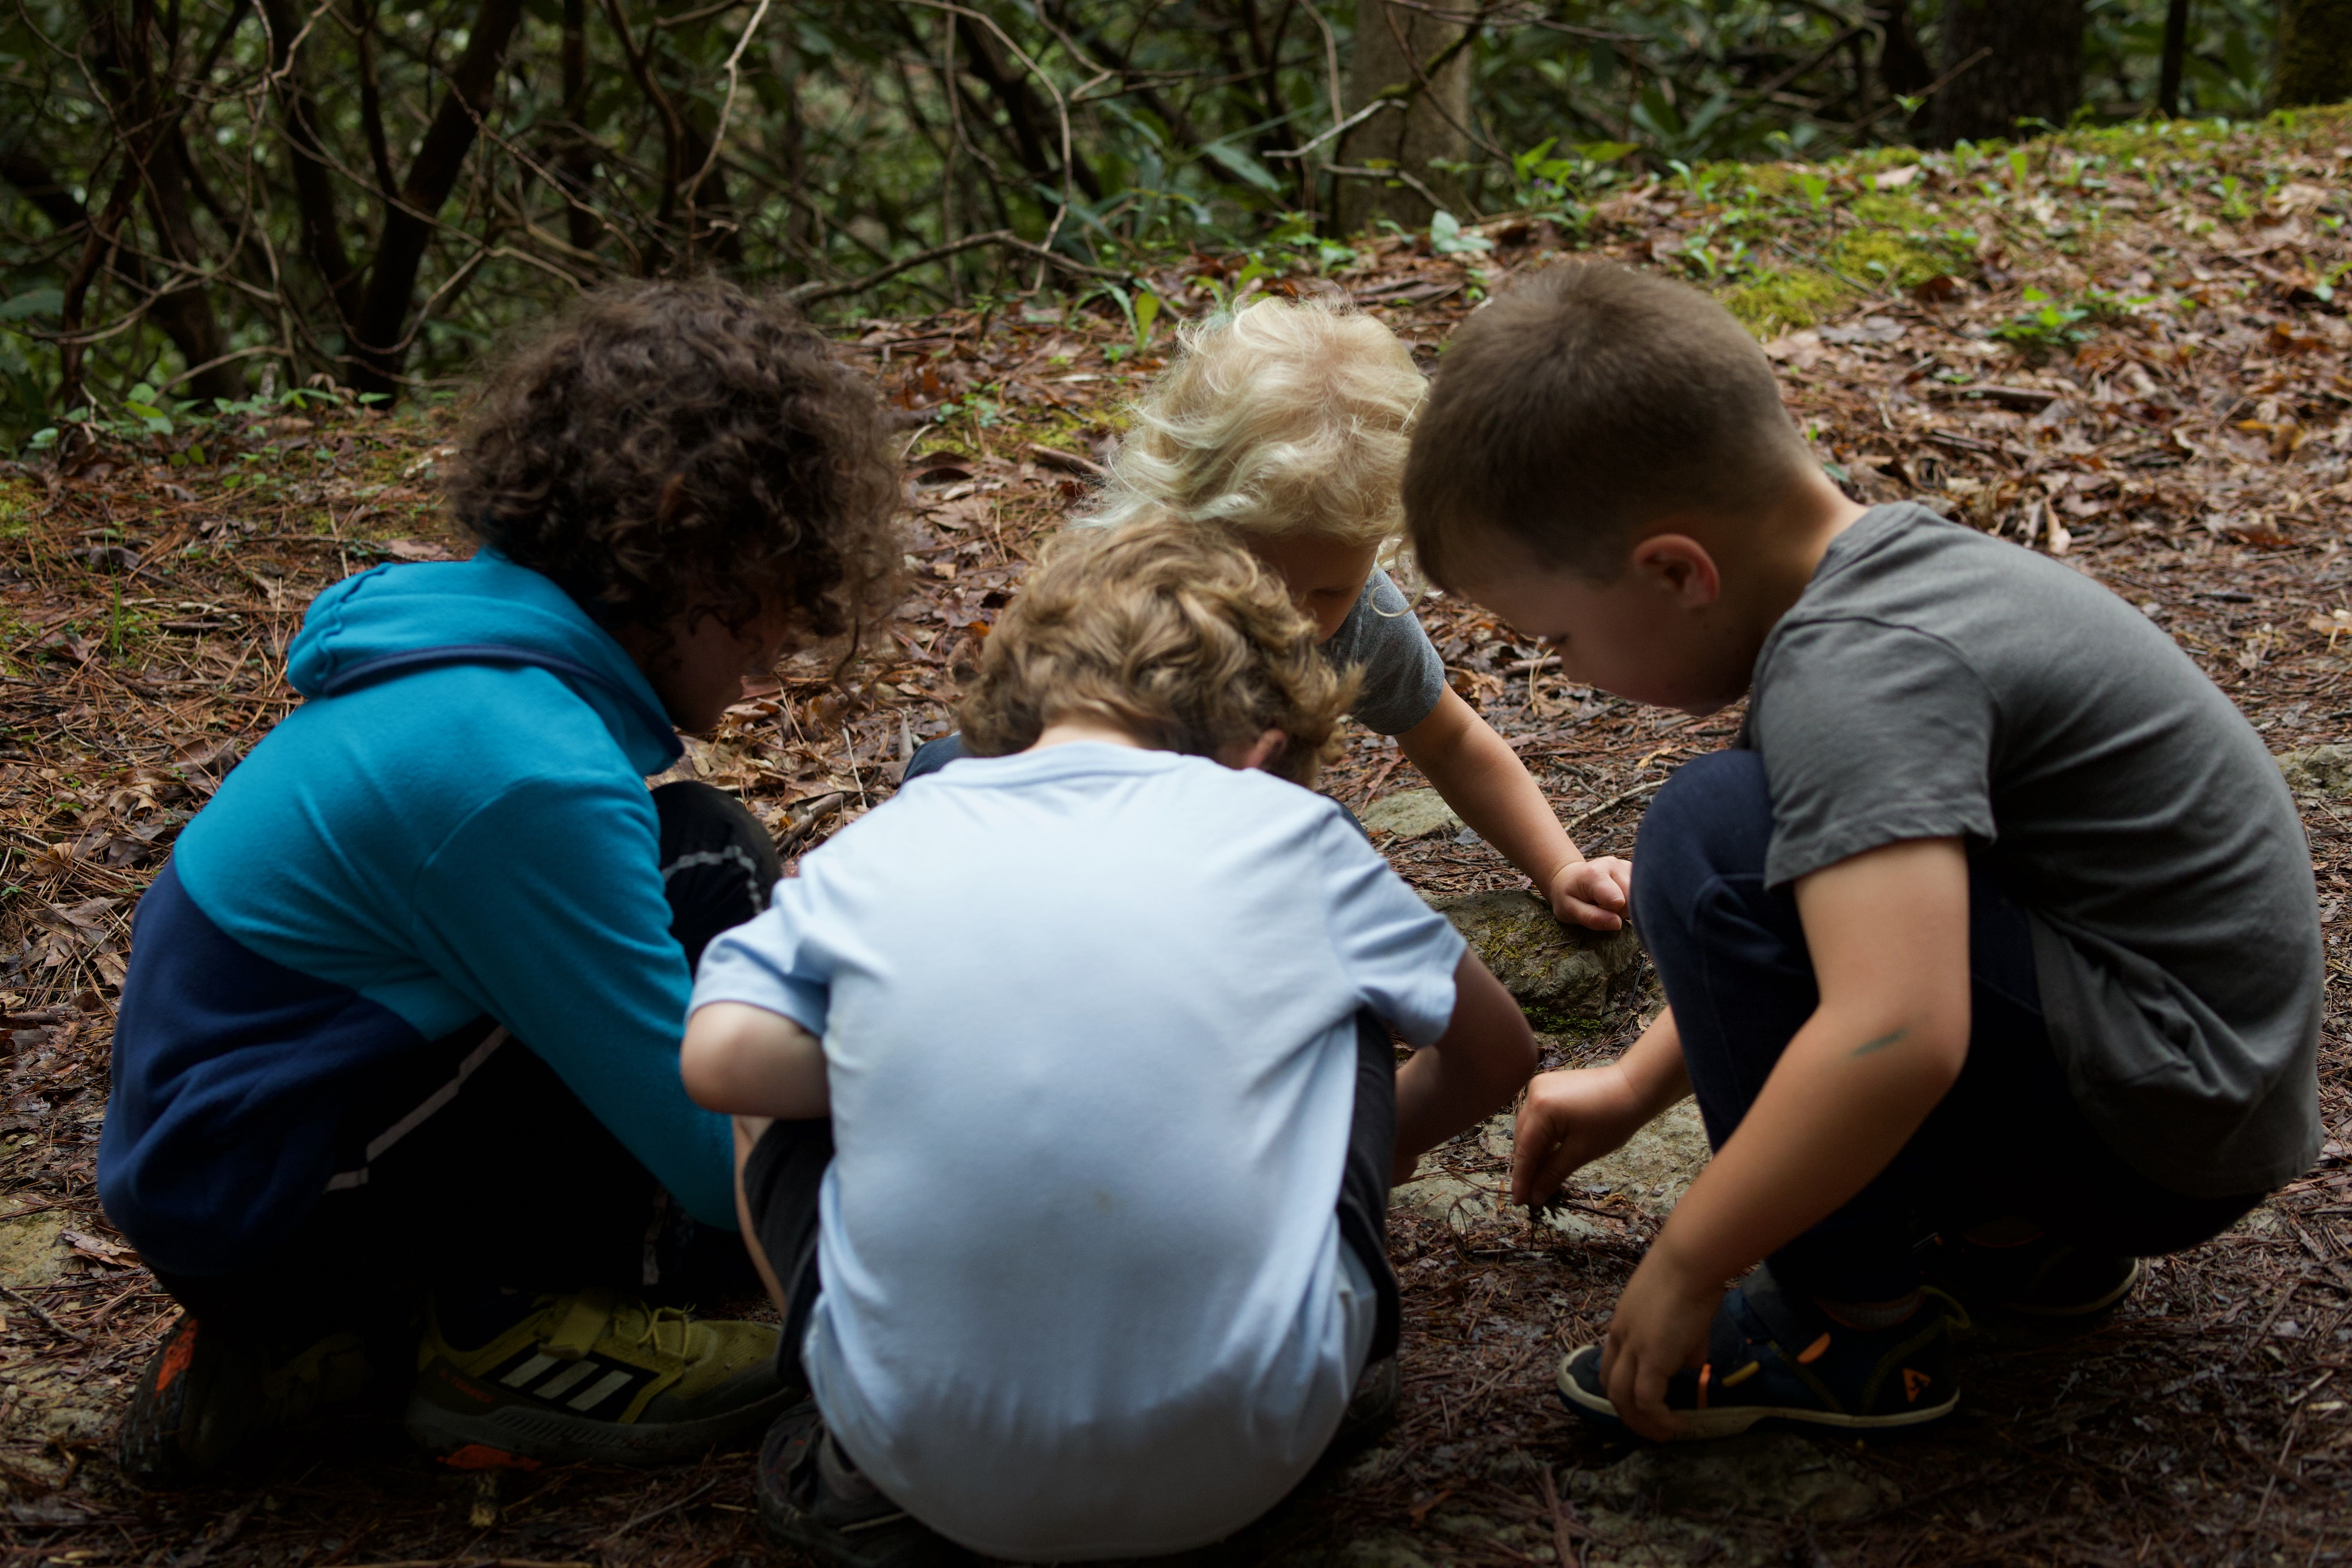
\includegraphics{img/kidslooking.jpg}

Plan for the basics. Take a look at the weather for the area or region
you're hiking, get a gauge on the terrain, and wear or pack appropriate
clothes and shoes. Oh, and snacks. Lots of snacks!

Plan for a mess.

When a kiddo plods through a creek, it sure is nice to have a backup
pair of socks and shoes! Sometimes, an emergency change of clothes
packed in your bag or in your car can come in handy. Some bandaids or a
basic first aid kit is always nice to have in a pinch and, in general,
bring more water than you think you'll need, because you never know!

!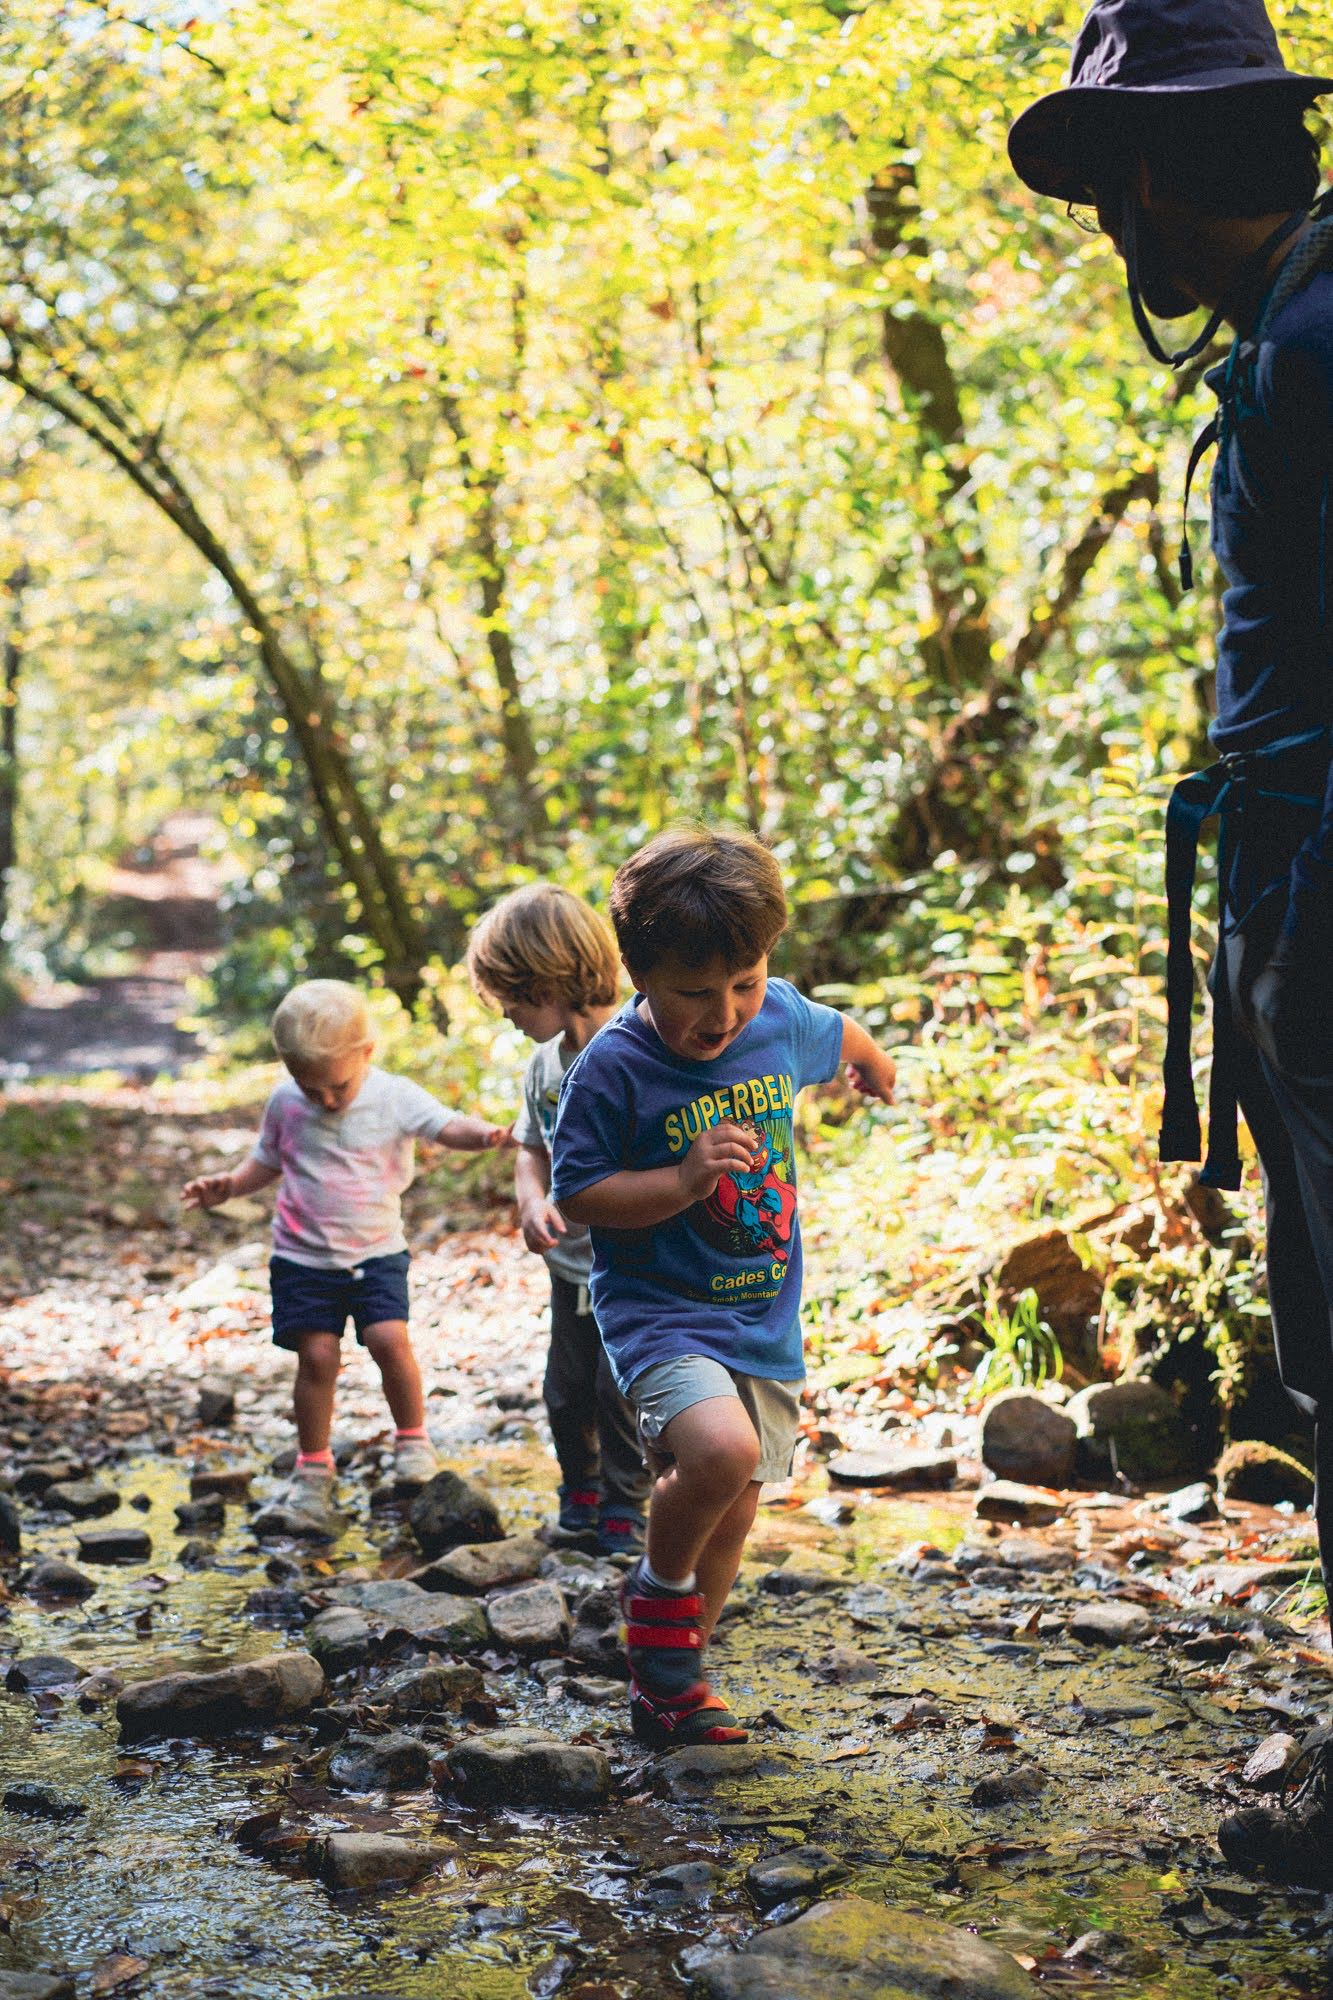
\includegraphics{img/kidscrossingcreek.jpg}

Embrace serendipity. It's good to have a plan, but don't be surprised if
something better comes along! Maybe you hike further than you thought
you would, or perhaps your child surprises you (and themselves!) by
taking some time to rock hop across a creek or explore animal tracks.

\hypertarget{introduction}{%
\subsection{Introduction}\label{introduction}}

These hikes are within or near Knoxville, in what is often referred to
as the Tennessee Valley. The Tennessee Valley includes Knoxville and
many other cities that border the mountains that surround Knoxville.
This area is known as the Tennessee Valley because of its primary
geographic feature: The Tennessee River.

The Tennessee River begins just beyond the city limits of Knoxville,
where the Holston and the French Broad Rivers meet. It (literally and
figuratively!) contains fewer high points than the Cumberland Plateau
and the Great Smoky Mountains, but, it should not be discounted as a
destination for hiking.

We think a trip to Seven Islands State Birding Park will make how
spectactular this area can be evident. Around 30 minutes away from most
places in Knoxville, this is a true destination for not only birders,
but also hikers and paddlers.

Other locations are also not only close, but (surprisingly) worthy of a
trip. Ijams on the south side of Knoxville--familiar to many in the
Knoxville area--has many spectacular features, in addition to being
fewer than ten minutes away from downtown.

Other places that we highlight are also worth your time, offering an
outdoors respite in addition to the ability to easily be integrated into
busy schedules and other commitments. If you are looking for a first
family hike, those in this section may make a great selection.

\hypertarget{trail-1-seven-islands}{%
\subsection{Trail 1: Seven Islands}\label{trail-1-seven-islands}}

\hypertarget{key-characteristics}{%
\subsubsection{Key Characteristics}\label{key-characteristics}}

\begin{longtable}[]{@{}
  >{\raggedright\arraybackslash}p{(\columnwidth - 2\tabcolsep) * \real{0.5000}}
  >{\raggedright\arraybackslash}p{(\columnwidth - 2\tabcolsep) * \real{0.5000}}@{}}
\toprule\noalign{}
\begin{minipage}[b]{\linewidth}\raggedright
Trail Name
\end{minipage} & \begin{minipage}[b]{\linewidth}\raggedright
Seven Islands Loop
\end{minipage} \\
\midrule\noalign{}
\endhead
\bottomrule\noalign{}
\endlastfoot
Region & Knoxville and Surroundings \\
Trail \# & 1 \\
Time Estimate - Hiking Fast & 1.5 hours \\
Time Estimate - Hiking Slowly & 3 hours \\
Trail Distance (Miles) & 2.3 \\
Elevation Change & Gentle \\
Pets & Allowed on leash \\
Parking Pass/Entrance Fee & Not Required \\
Restroom(s) & Yes \\
Terrain & Paved; dirt path \\
Trailhead Address & Seven Islands State Birding Park, 2809 Kelly Ln,
Kodak, TN 37764 \\
Trailhead GPS Coordinates & 35.95366, -83.68701 \\
\end{longtable}

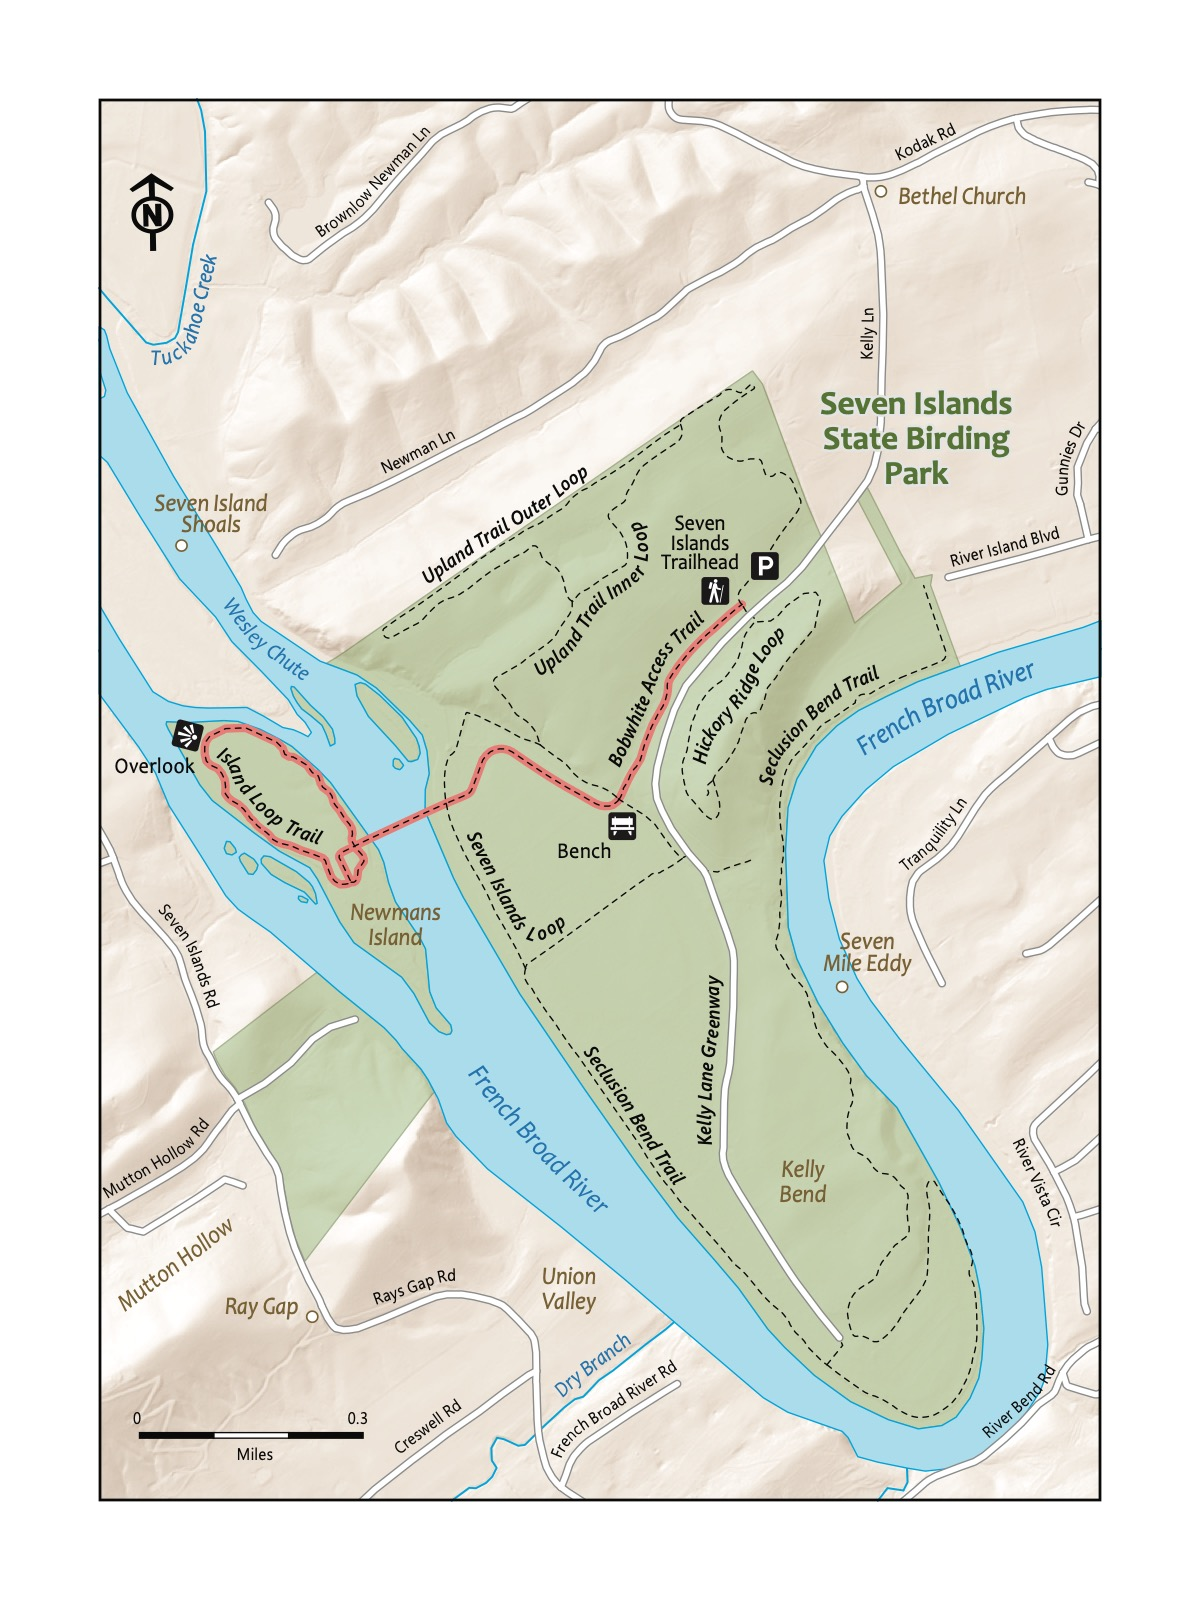
\includegraphics{maps/trail-01-map.jpeg}

\hypertarget{overview}{%
\subsubsection{Overview}\label{overview}}

This is one of our favorite trails in this book---it is the first trail
for that reason. Even though it is relatively close to Knoxville, it is
simply a fantastic place to hike. For the trail we highlight, a paved
path descends through a meadow. Look for birds and deer! The trail
crosses a bridge over the French Broad River and hike around a beautiful
island (look for side trails and the native paw paw fruit in the fall!)
before returning to the start---or pick one of the many other nearby
trails in the park. Great for all ages and seasons, though sometimes hot
in the summer due to limited shade on the paved part of the trail.

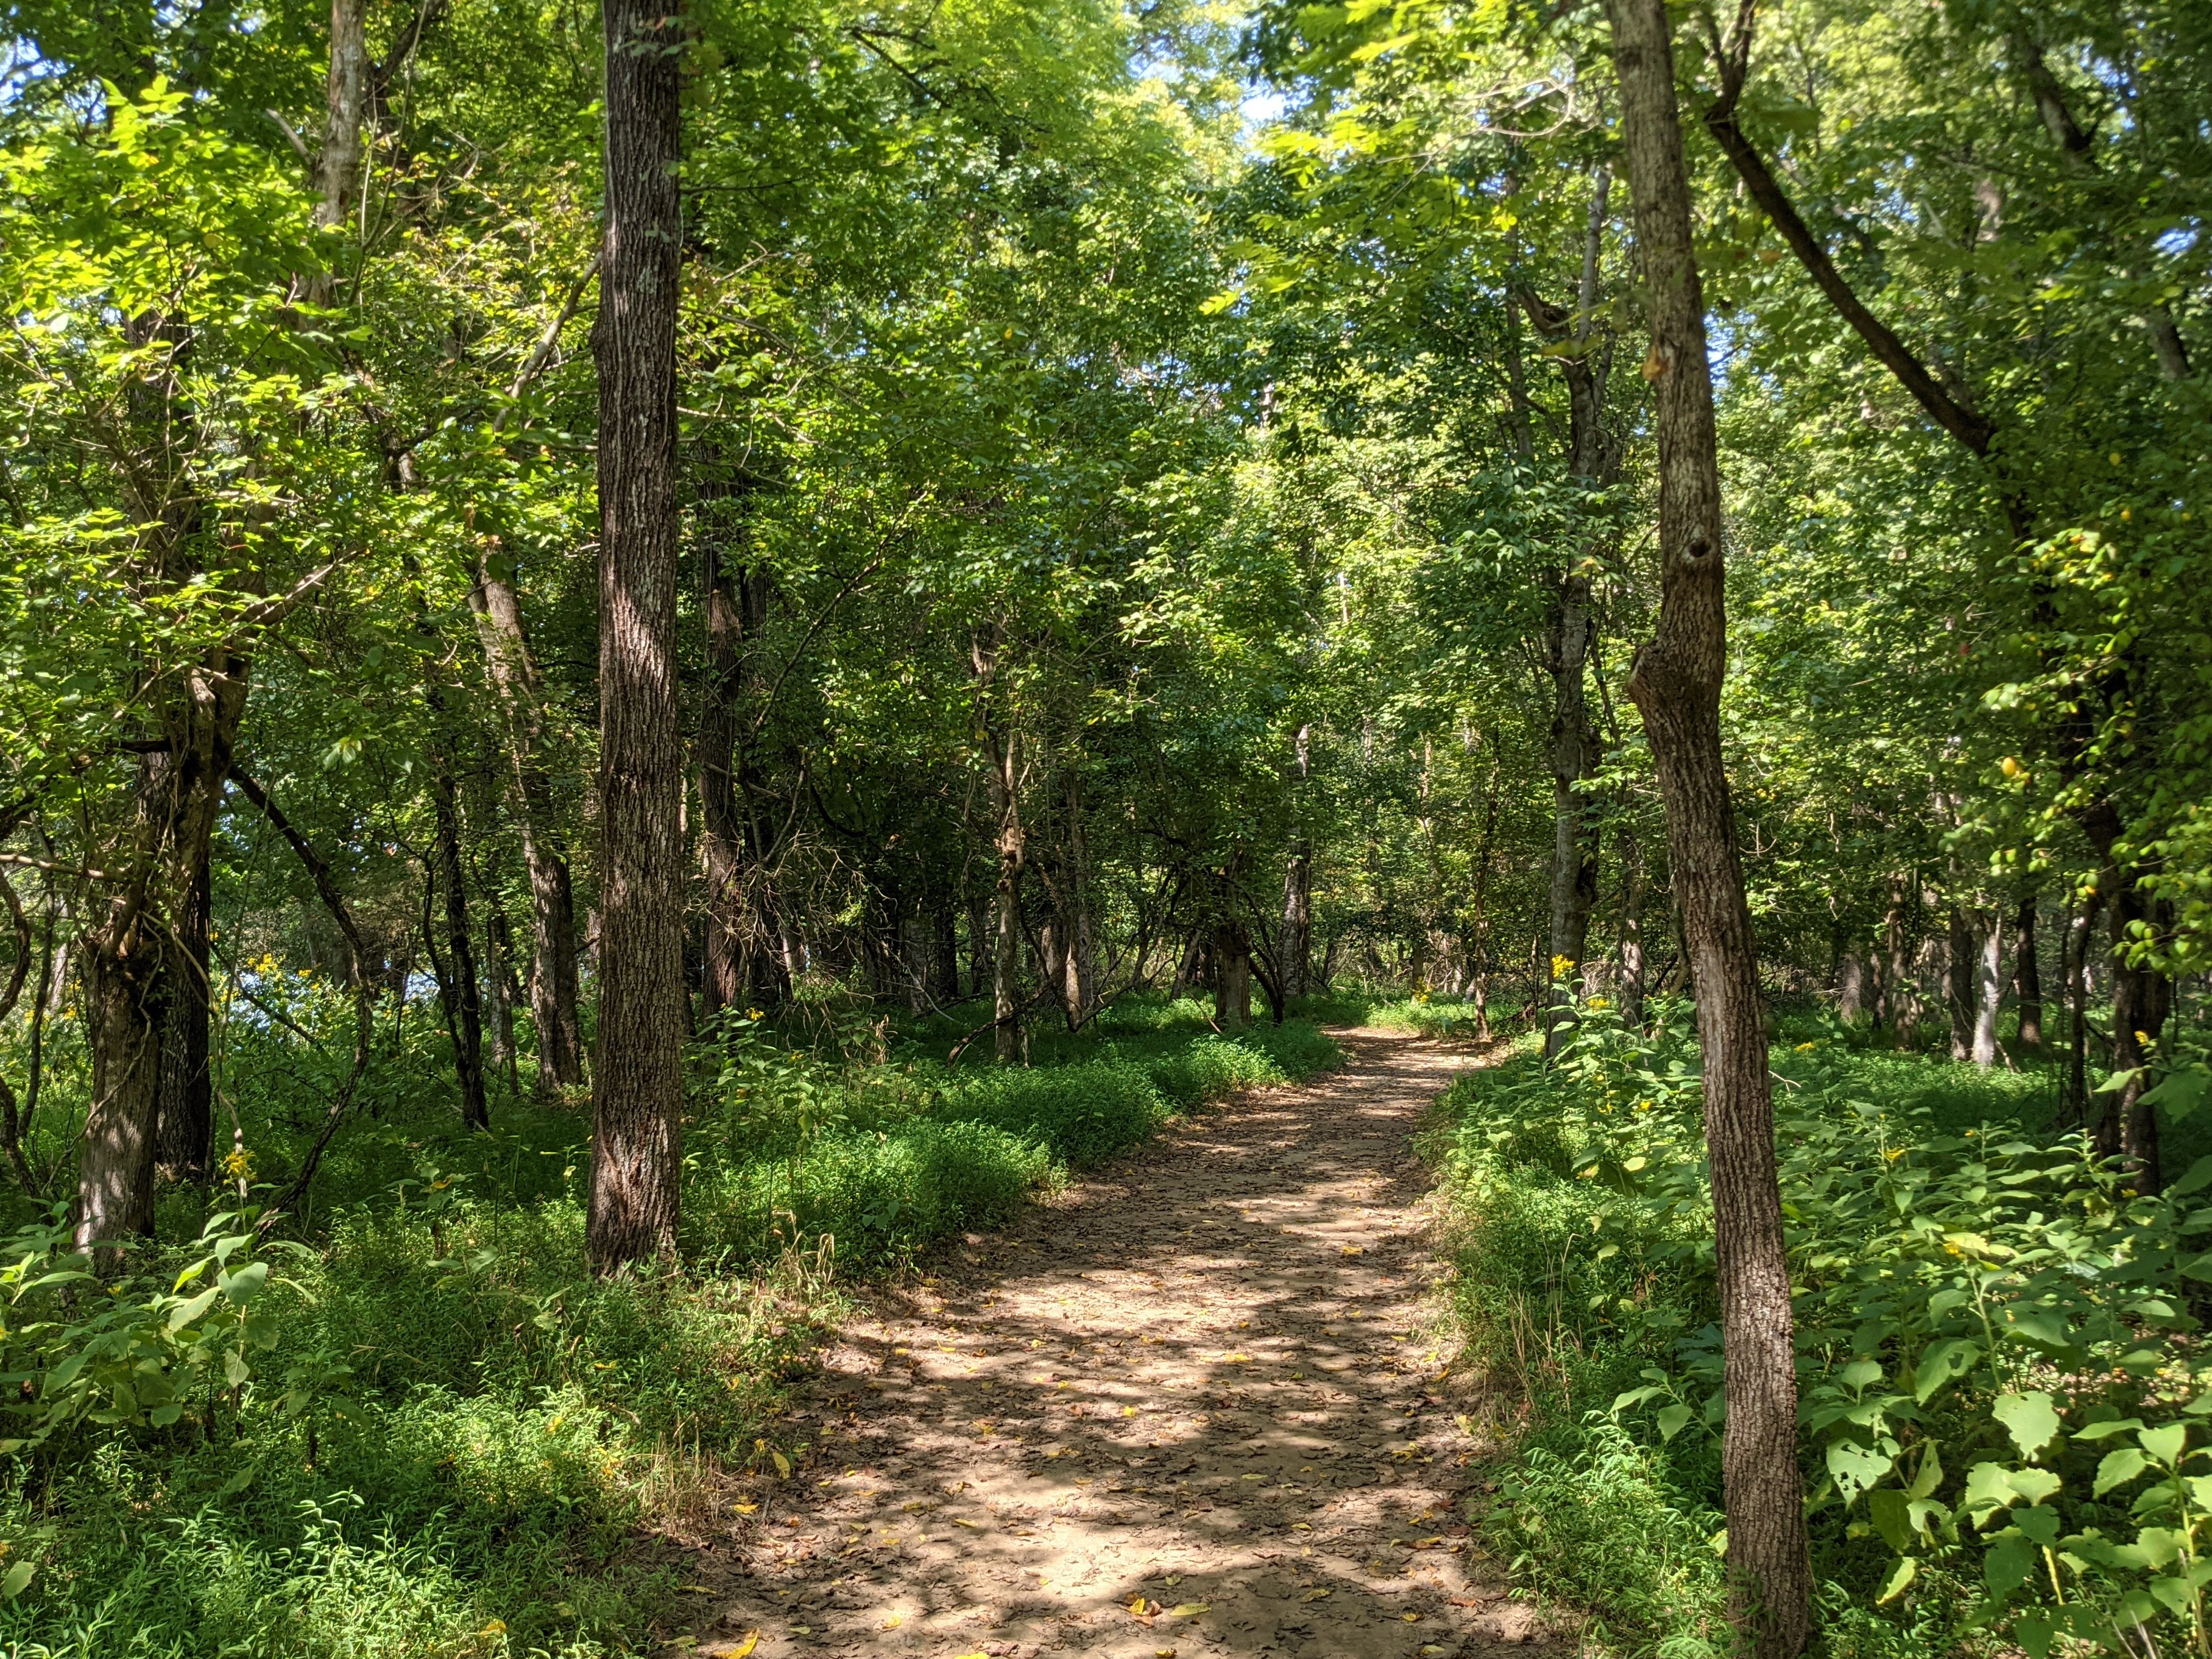
\includegraphics{img/trail-01-figure-01.jpg}

\hypertarget{directions-to-the-trailhead}{%
\subsubsection{Directions to the
Trailhead}\label{directions-to-the-trailhead}}

Trailhead Address \textbar{} Seven Islands State Birding Park, 2809
Kelly Ln, Kodak, TN 37764 \textbar{}\\
\strut \\
\strut \\
Trailhead GPS Coordinates \textbar{} 35.95366, -83.68701\\
\strut \\

Navigate using the above address to the main parking area (note there is
another parking area by a boat launch that is not the correct location
for this hike!). Park in the large gravel lot. We have never had trouble
finding a spot even on the busiest of days. The address of the parking
lot at Seven Islands is: 2809 Kelly Ln., Kodak, TN 37764.

\hypertarget{trail-description}{%
\subsubsection{Trail Description}\label{trail-description}}

\begin{longtable}[]{@{}
  >{\raggedright\arraybackslash}p{(\columnwidth - 2\tabcolsep) * \real{0.5000}}
  >{\raggedright\arraybackslash}p{(\columnwidth - 2\tabcolsep) * \real{0.5000}}@{}}
\toprule\noalign{}
\begin{minipage}[b]{\linewidth}\raggedright
Distance from Start
\end{minipage} & \begin{minipage}[b]{\linewidth}\raggedright
Description
\end{minipage} \\
\midrule\noalign{}
\endhead
\bottomrule\noalign{}
\endlastfoot
0.0 & Barn with the blue ``barn quilt'' featuring four blue birds. You
can walk through the barn to begin the hike on the paved Bobwhite Access
trail. \\
0.05 & Bathroom on the left of the trail. \\
0.1 & Descend through grassy meadows with wildflowers in the spring and
early fall. \\
0.3 & Bench. \\
0.6 & Start of the Newmans Island Bridge. \\
0.8 & End of the bridge. Paved trail ends. Turn right onto the Island
Loop Trail to hike around the island in a clockwise direction. \\
0.85 & Picnic table beside a pretty part of the French Broad River. \\
1.05 & Stick house (kiddo favorite!). \\
1.5 & Connect back to the bridge, heading back onto the Bobwhite Access
Trail. \\
2 & Climb back up past the meadows. This is the toughest part of the
hike (but, it shouldn't be too steep, and the trailhead is near!). \\
2.3 & Trailhead. \\
\end{longtable}

\hypertarget{nearby}{%
\subsubsection{Nearby}\label{nearby}}

\begin{itemize}
\tightlist
\item
  Hiking other trails. Hike up the Hickory Ridge trail, another trail at
  Seven Islands State Birding Park that is accessible from just behind
  the bathrooms near the parking lot. There are several other great
  hikes available, including hikes down the Kelly Lane Greenway (the
  other, wider, paved path near the barn that is gated to prevent cars
  from driving on it) and the Upland Inner and Outer Trail Loops.
\item
  Enjoying watersports. Consider kayaking, canoeing, or paddleboarding,
  especially on warm days. There is a great place to put in, Seven
  Islands Landing and Boat Ramp (2809 Kelly Ln, Kodak, TN 37764). Also,
  River Sports Outfitters rents kayaks and canoes here during the summer
  (see \url{https://www.riversportsoutfitters.com/}).\\
\item
  Stopping for a bite to eat and a drink on the way back. On the way
  home, consider stopping by kid-friendly Walnut Springs Winery (1175
  Midway Rd, Knoxville, TN 37914), open Wednesday-Sunday as of this
  writing.
\end{itemize}

\hypertarget{trail-2-ijams-riverside}{%
\subsection{Trail 2: Ijams Riverside}\label{trail-2-ijams-riverside}}

\hypertarget{key-characteristics-1}{%
\subsubsection{Key Characteristics}\label{key-characteristics-1}}

\begin{longtable}[]{@{}
  >{\raggedright\arraybackslash}p{(\columnwidth - 2\tabcolsep) * \real{0.6111}}
  >{\raggedright\arraybackslash}p{(\columnwidth - 2\tabcolsep) * \real{0.3889}}@{}}
\toprule\noalign{}
\begin{minipage}[b]{\linewidth}\raggedright
Distance from Start
\end{minipage} & \begin{minipage}[b]{\linewidth}\raggedright
Description
\end{minipage} \\
\midrule\noalign{}
\endhead
\bottomrule\noalign{}
\endlastfoot
0.0 & Start near the doors to the Visitor's Center. \\
0.05 & Turn left to begin the North Cove Trail. \\
0.2 & Turn right onto the River Trail. \\
0.4 & Short wooden stairs down to the boardwalk section. \\
0.5 & End of the boardwalk section. \\
0.6 & Climb rock steps. \\
0.7 & Turn right on the Tower Trail (or, optionally, remain on the River
Trail to head toward Mead's Quarry). \\
0.85 & Pass an old communication tower at the high point of the trail;
begin to descend back to the Visitor's Center. \\
1.03 & Return to the Visitor's Center. \\
\end{longtable}

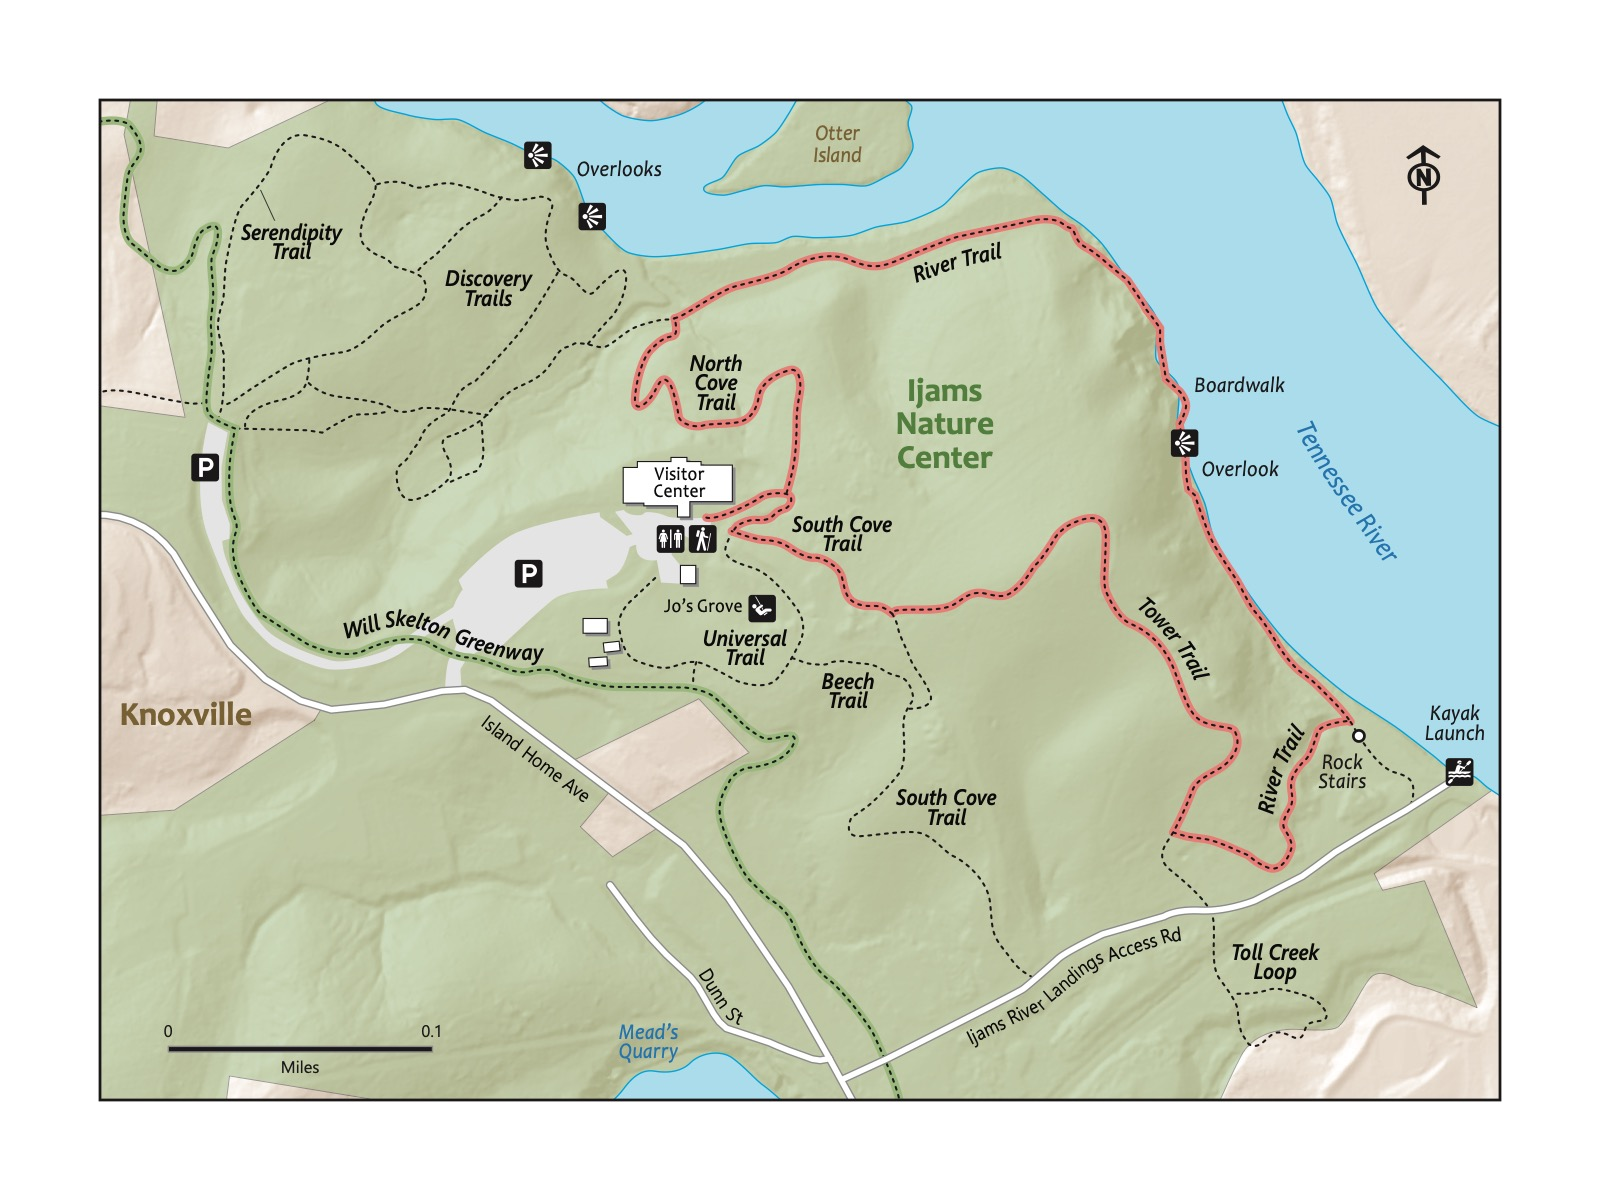
\includegraphics{maps/trail-02-map.jpeg}

\hypertarget{overview-1}{%
\subsubsection{Overview}\label{overview-1}}

If you live in Knoxville, then you've probably heard of Ijams Nature
Center. It's easy to take for granted, but we seem to find something new
every time we visit --- and we always have a great time. This hike is
meant to be a gentle introduction to what Ijams refers to as the
Riverside area (see the Ijams Crag hike for an introduction to the
second part of Ijams). The trail starts by the Ijams Nature Center's
visitor center and hikes down through a deep forest to the river. It
continues along the boardwalk trail that happens to follow the side of
the very first mile of the Tennessee River. The trail returns back up
and over a rocky ridge to return to the visitor center---and the play
area and links to other trails nearby.

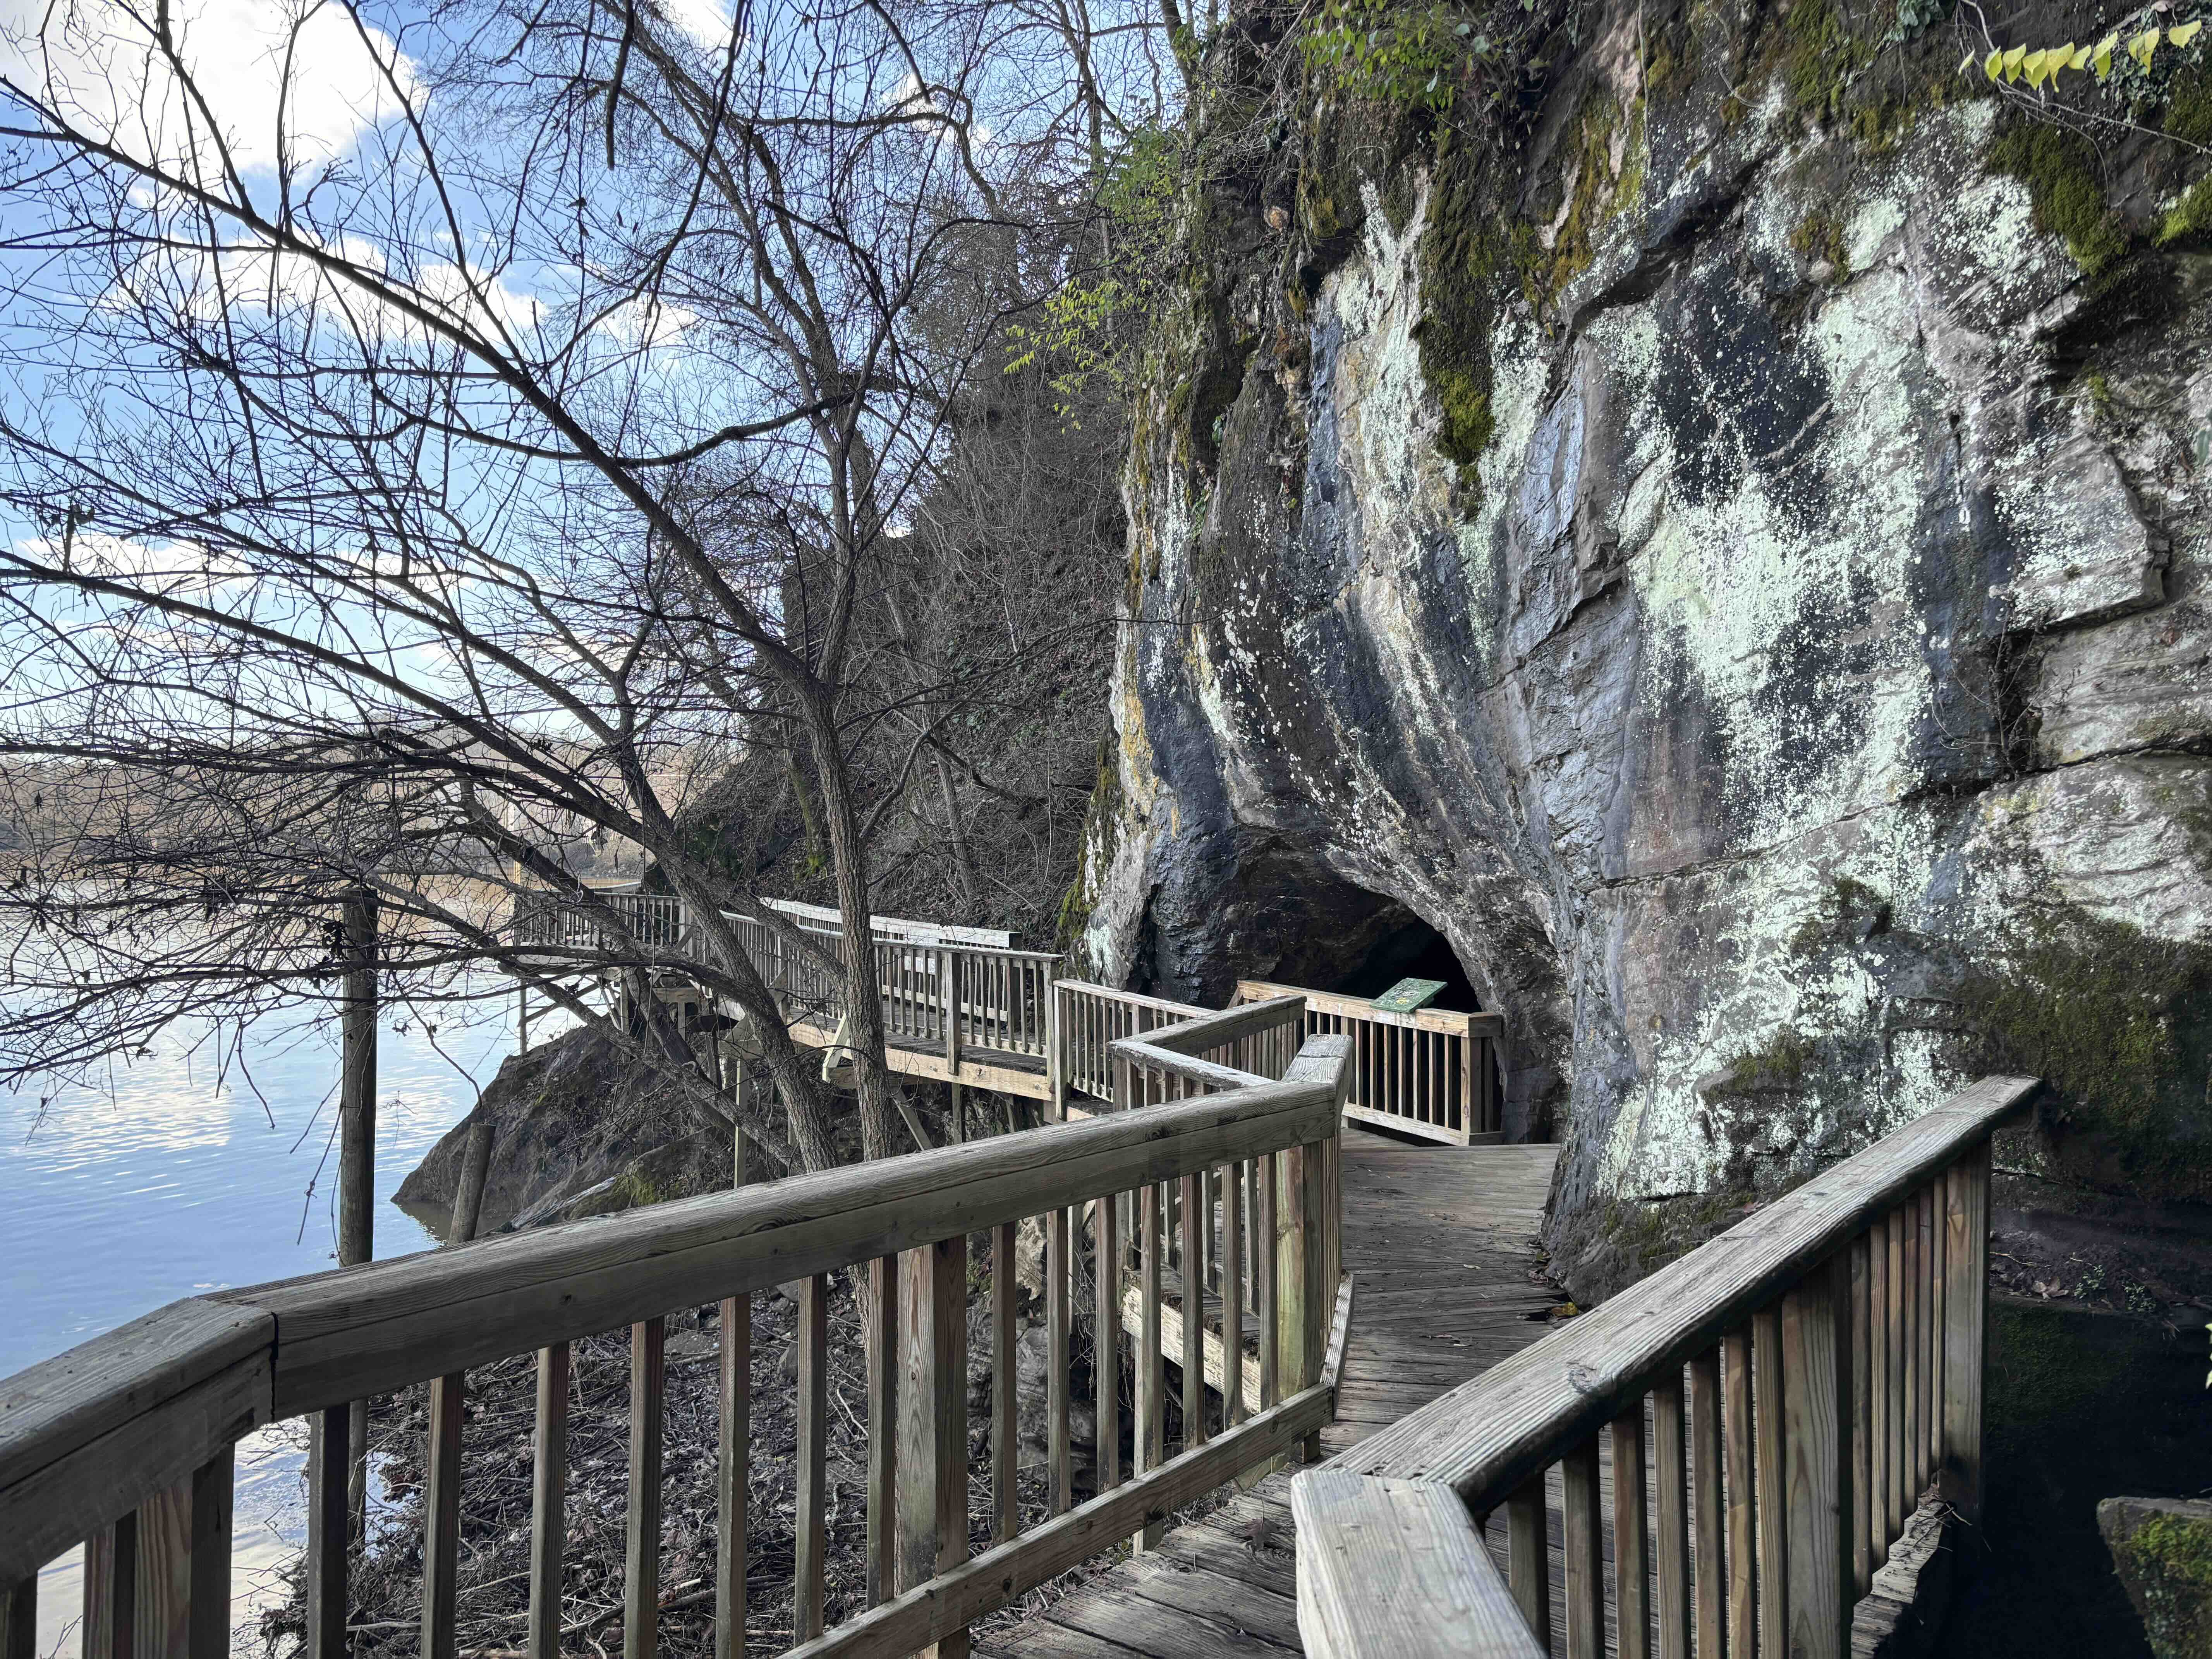
\includegraphics{img/trail-02-figure-01.jpg}

\hypertarget{directions-to-the-trailhead-1}{%
\subsubsection{Directions to the
Trailhead}\label{directions-to-the-trailhead-1}}

\begin{longtable}[]{@{}
  >{\raggedright\arraybackslash}p{(\columnwidth - 2\tabcolsep) * \real{0.5000}}
  >{\raggedright\arraybackslash}p{(\columnwidth - 2\tabcolsep) * \real{0.5000}}@{}}
\toprule\noalign{}
\begin{minipage}[b]{\linewidth}\raggedright
Trailhead Address
\end{minipage} & \begin{minipage}[b]{\linewidth}\raggedright
Ijams Nature Center, 2915 Island Home Ave, Knoxville, TN 37920
\end{minipage} \\
\midrule\noalign{}
\endhead
\bottomrule\noalign{}
\endlastfoot
Trailhead GPS Coordinates & 35.95612, -83.86725 \\
\end{longtable}

:----- \textbar{} :----- \textbar{}\\
\strut \\
\strut \\
\hspace*{0.333em}\textbar{} Use the above address easily navigate you to
the parking area. Park in the large parking lot near the Visitor's
Center. Look for signs for the North Cove Trail; looking toward the
front doors to the Visitor's Center, the trail heads off to the right.
\textbar{}\\
\strut \\

\hypertarget{trail-description-1}{%
\subsubsection{Trail Description}\label{trail-description-1}}

\begin{longtable}[]{@{}
  >{\raggedright\arraybackslash}p{(\columnwidth - 2\tabcolsep) * \real{0.6111}}
  >{\raggedright\arraybackslash}p{(\columnwidth - 2\tabcolsep) * \real{0.3889}}@{}}
\toprule\noalign{}
\begin{minipage}[b]{\linewidth}\raggedright
Distance from Start
\end{minipage} & \begin{minipage}[b]{\linewidth}\raggedright
Description
\end{minipage} \\
\midrule\noalign{}
\endhead
\bottomrule\noalign{}
\endlastfoot
0.0 & Start near the doors to the Visitor's Center. \\
0.05 & Turn left to begin the North Cove Trail. \\
0.2 & Turn right onto the River Trail. \\
0.4 & Short wooden stairs down to the boardwalk section. \\
0.5 & End of the boardwalk section. \\
0.6 & Climb rock steps. \\
0.7 & Turn right on the Tower Trail (or, optionally, remain on the River
Trail to head toward Mead's Quarry). \\
0.85 & Pass an old communication tower at the high point of the trail;
begin to descend back to the Visitor's Center. \\
1.03 & Return to the Visitor's Center. \\
\end{longtable}

\hypertarget{nearby-1}{%
\subsubsection{Nearby}\label{nearby-1}}

\begin{itemize}
\tightlist
\item
  Hiking at Mead's Quarry. Check out the Ijams Crag hike for a great
  starting point at the over area that comprises Ijams.
\item
  Visit Jo's Grove. Near the Visitor's Center, which features a fun
  cabin and a wooded area for kids to play and goof (this is a premiere
  hide-and-seek spot!).
\item
  Grabbing a bite to eat on the south side of Knoxville. The south side
  of town near Ijams is a great place to grab a bite to eat. Our
  favorites include South Coast Pizza (1103 Sevier Ave, Knoxville, TN
  37920) and Angry Dumplings Tea (1119 Sevier Ave, Knoxville, TN 37920).
  Breweries nearby also abound.
\end{itemize}

\hypertarget{trail-3-lakeshore-park}{%
\subsection{Trail 3: Lakeshore Park}\label{trail-3-lakeshore-park}}

\hypertarget{key-characteristics-2}{%
\subsubsection{Key Characteristics}\label{key-characteristics-2}}

\begin{longtable}[]{@{}ll@{}}
\toprule\noalign{}
Trail Name & Lakeshore Park \\
\midrule\noalign{}
\endhead
\bottomrule\noalign{}
\endlastfoot
Region & Knoxville and Surroundings \\
Trail \# & 3 \\
Time Estimate - Hiking Fast & 1.5 hours \\
Time Estimate - Hiking Slowly & 2.5 hours \\
Trail Distance (Miles) & 2.2 \\
Elevation Change & Gentle \\
Pets & Allowed on leash \\
Parking Pass/Entrance Fee & Not Required \\
Restroom(s) & Yes \\
Terrain & Paved \\
\end{longtable}

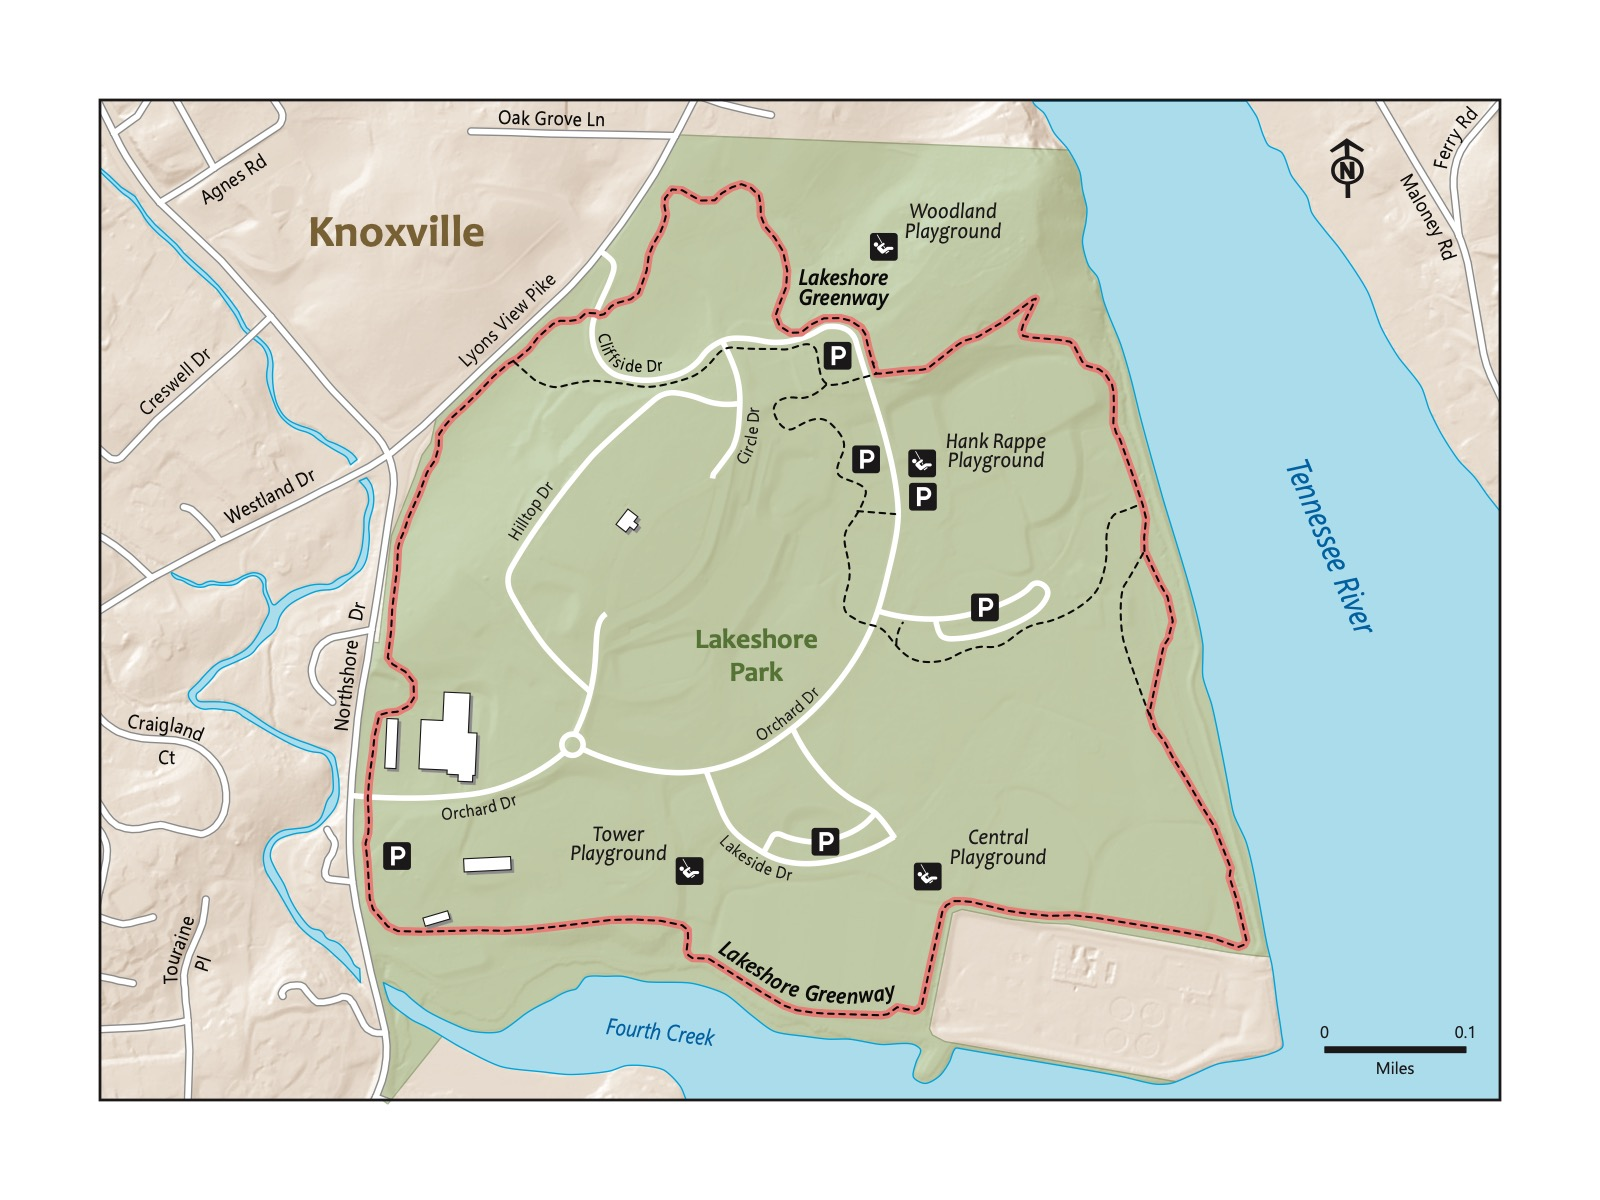
\includegraphics{maps/trail-03-map.jpeg}

\hypertarget{overview-2}{%
\subsubsection{Overview}\label{overview-2}}

A gem in Knoxville's city park system. This hike, entirely on a paved
path, circles the perimeter of the park, featuring high points (and
views of the Smokies) and a boardwalk along the river. Traverses past
four excellent play areas this hike winds past. Well known, but not
overrated --- a great spot for a hike that could fit into a busy
weekend, or even a weeknight. Good for kids of all ages; consider
looping back to your start point with younger children.

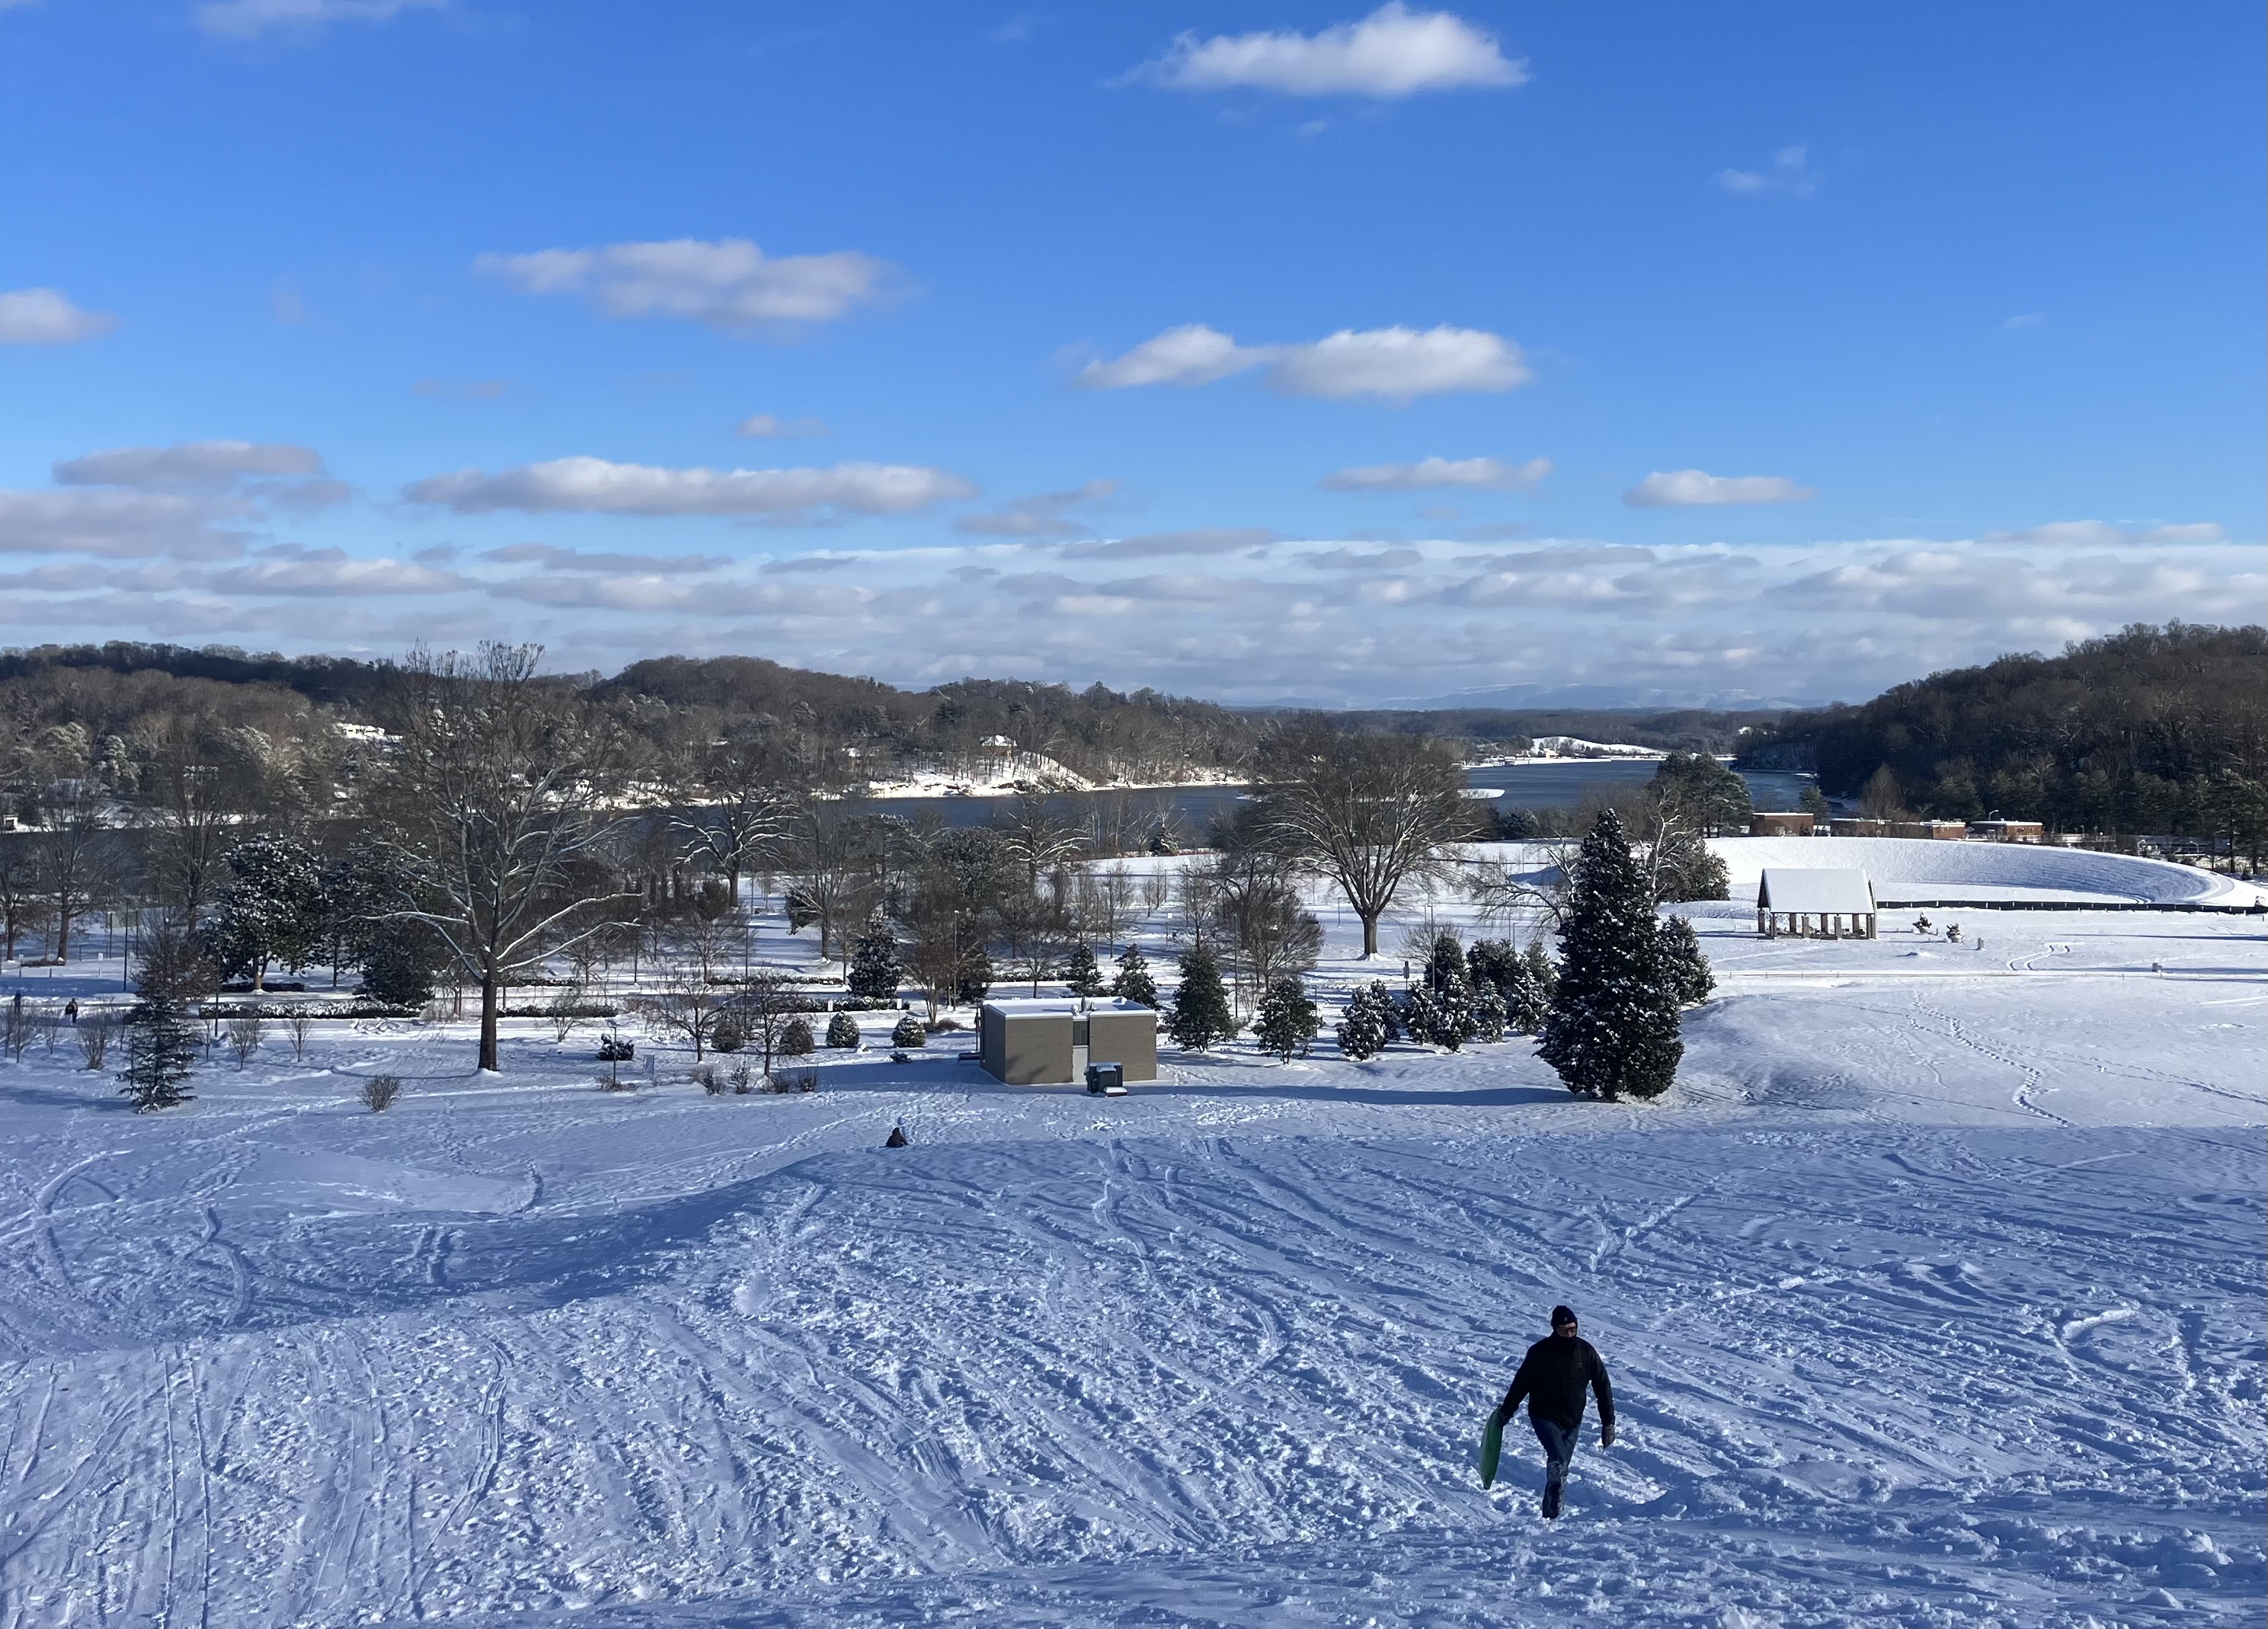
\includegraphics{img/trail-03-figure-01.jpg}

\hypertarget{directions-to-the-trailhead-2}{%
\subsubsection{Directions to the
Trailhead}\label{directions-to-the-trailhead-2}}

\begin{longtable}[]{@{}
  >{\raggedright\arraybackslash}p{(\columnwidth - 2\tabcolsep) * \real{0.5000}}
  >{\raggedright\arraybackslash}p{(\columnwidth - 2\tabcolsep) * \real{0.5000}}@{}}
\toprule\noalign{}
\begin{minipage}[b]{\linewidth}\raggedright
Trailhead Address
\end{minipage} & \begin{minipage}[b]{\linewidth}\raggedright
Lakeshore Park, 6014 Lyons View Pike, Knoxville, TN 37919
\end{minipage} \\
\midrule\noalign{}
\endhead
\bottomrule\noalign{}
\endlastfoot
Trailhead GPS Coordinates & 35.92389, -83.990 \\
\end{longtable}

The address above is suitable for navigating to Lakeshore in general,
but it's a large park! Our hike starts at a large parking area near the
center of the park. To find it, entering Lakeshor from Lyons View Pike,
turn left onto Cliffside Dr., and park in the large parking area on the
right, immediately past Circle Dr.~Start on the greenway near the
parking lot, on the same side of the road on which you are parked. Of
course, you can park elsewhere nearby or in any parking area at
Lakeshore.

\hypertarget{trail-description-2}{%
\subsubsection{Trail Description}\label{trail-description-2}}

\begin{longtable}[]{@{}
  >{\raggedright\arraybackslash}p{(\columnwidth - 2\tabcolsep) * \real{0.5000}}
  >{\raggedright\arraybackslash}p{(\columnwidth - 2\tabcolsep) * \real{0.5000}}@{}}
\toprule\noalign{}
\begin{minipage}[b]{\linewidth}\raggedright
Distance from Start
\end{minipage} & \begin{minipage}[b]{\linewidth}\raggedright
Description
\end{minipage} \\
\midrule\noalign{}
\endhead
\bottomrule\noalign{}
\endlastfoot
0.0 & Cross Orchard Drive, heading clockwise on the paved greenway. Note
the greenway on the left, which immediately heads toward the Huie
Woodland Playground. \\
0.05 & Bench and overlook to the Smokies. Can you spy Clingman's Dome?
Note that Hank Rappé playground is immediately below the greenway (to
your right). \\
0.15 & Steep descent! \\
0.4 & Optional boardwalk section (recommended!). Check out the viewing
platform overlooking the Tennessee River around 200 feet ahead on the
left. \\
0.5 & Boardwalk and the primary greenway reconnect. \\
& \\
0.9 & Central Playground on the right. \\
1.2 & Tower Playground on the right. \\
1.5 & Ascent (followed by a little hill back down) begins. \\
2.2 & Traihead. \\
\end{longtable}

\hypertarget{nearby-2}{%
\subsubsection{Nearby}\label{nearby-2}}

\begin{itemize}
\tightlist
\item
  Playing at one of the many playgrounds. There are four awesome
  playgrounds at Lakeshore --- Hank Rappé (universal playground with a
  bit of everything), Huie Woodland (nature-themed), Tower (lots of
  climbing opportunities!), and Central (smaller, and with workout
  equipment nearby).
\item
  Having a picnic. Lakeshore seems made for picnics. Bring one along for
  a grassy area or numerous seating areas near the Hank Rappé, Tower,
  and Central playgrounds.
\end{itemize}

\hypertarget{trail-4-high-ground-park}{%
\subsection{Trail 4: High Ground Park}\label{trail-4-high-ground-park}}

\hypertarget{key-characteristics-3}{%
\subsubsection{Key Characteristics}\label{key-characteristics-3}}

\begin{longtable}[]{@{}ll@{}}
\toprule\noalign{}
Trail Name & High Ground Park \\
\midrule\noalign{}
\endhead
\bottomrule\noalign{}
\endlastfoot
Region & Knoxville and Surroundings \\
Trail \# & 4 \\
Time Estimate - Hiking Fast & 0.5 hours \\
Time Estimate - Hiking Slowly & 1 hour \\
Trail Distance (Miles) & 0.7 \\
Elevation Change & Gentle \\
Pets & Allowed on leash \\
Parking Pass/Entrance Fee & Not Required \\
Restroom(s) & No \\
Terrain & Paved; dirt path \\
\end{longtable}

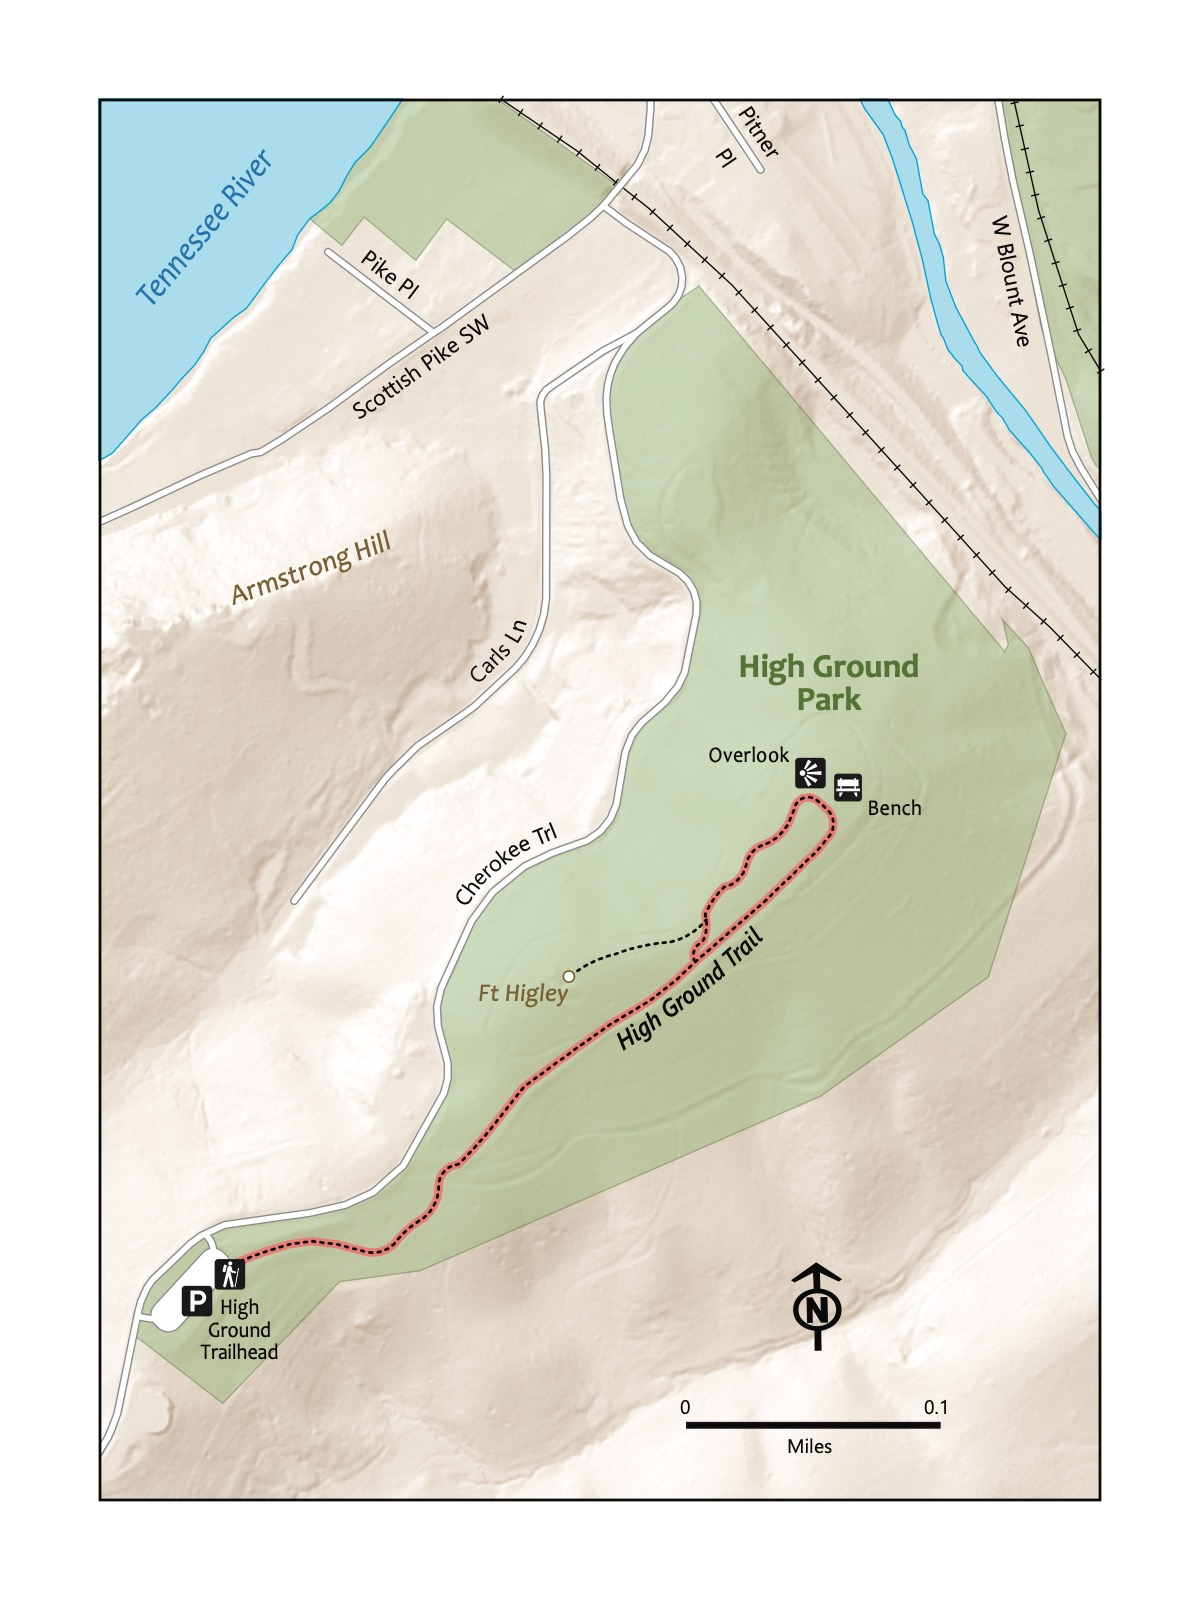
\includegraphics{maps/trail-04-map.jpeg}

\hypertarget{overview-3}{%
\subsubsection{Overview}\label{overview-3}}

It is one of the closest hikes to the city center of Knoxville --- and
one of a few that is highly stroller-friendly. This short but sweet hike
is perfect as a real but accessible outing for toddlers and little kids.
The red chairs at the top are a fun stopping point. The deep woods are
pretty in the fall. This could be a great first hike for toddlers---it
was one of the first for our little one, and we loved how accessible it
was.

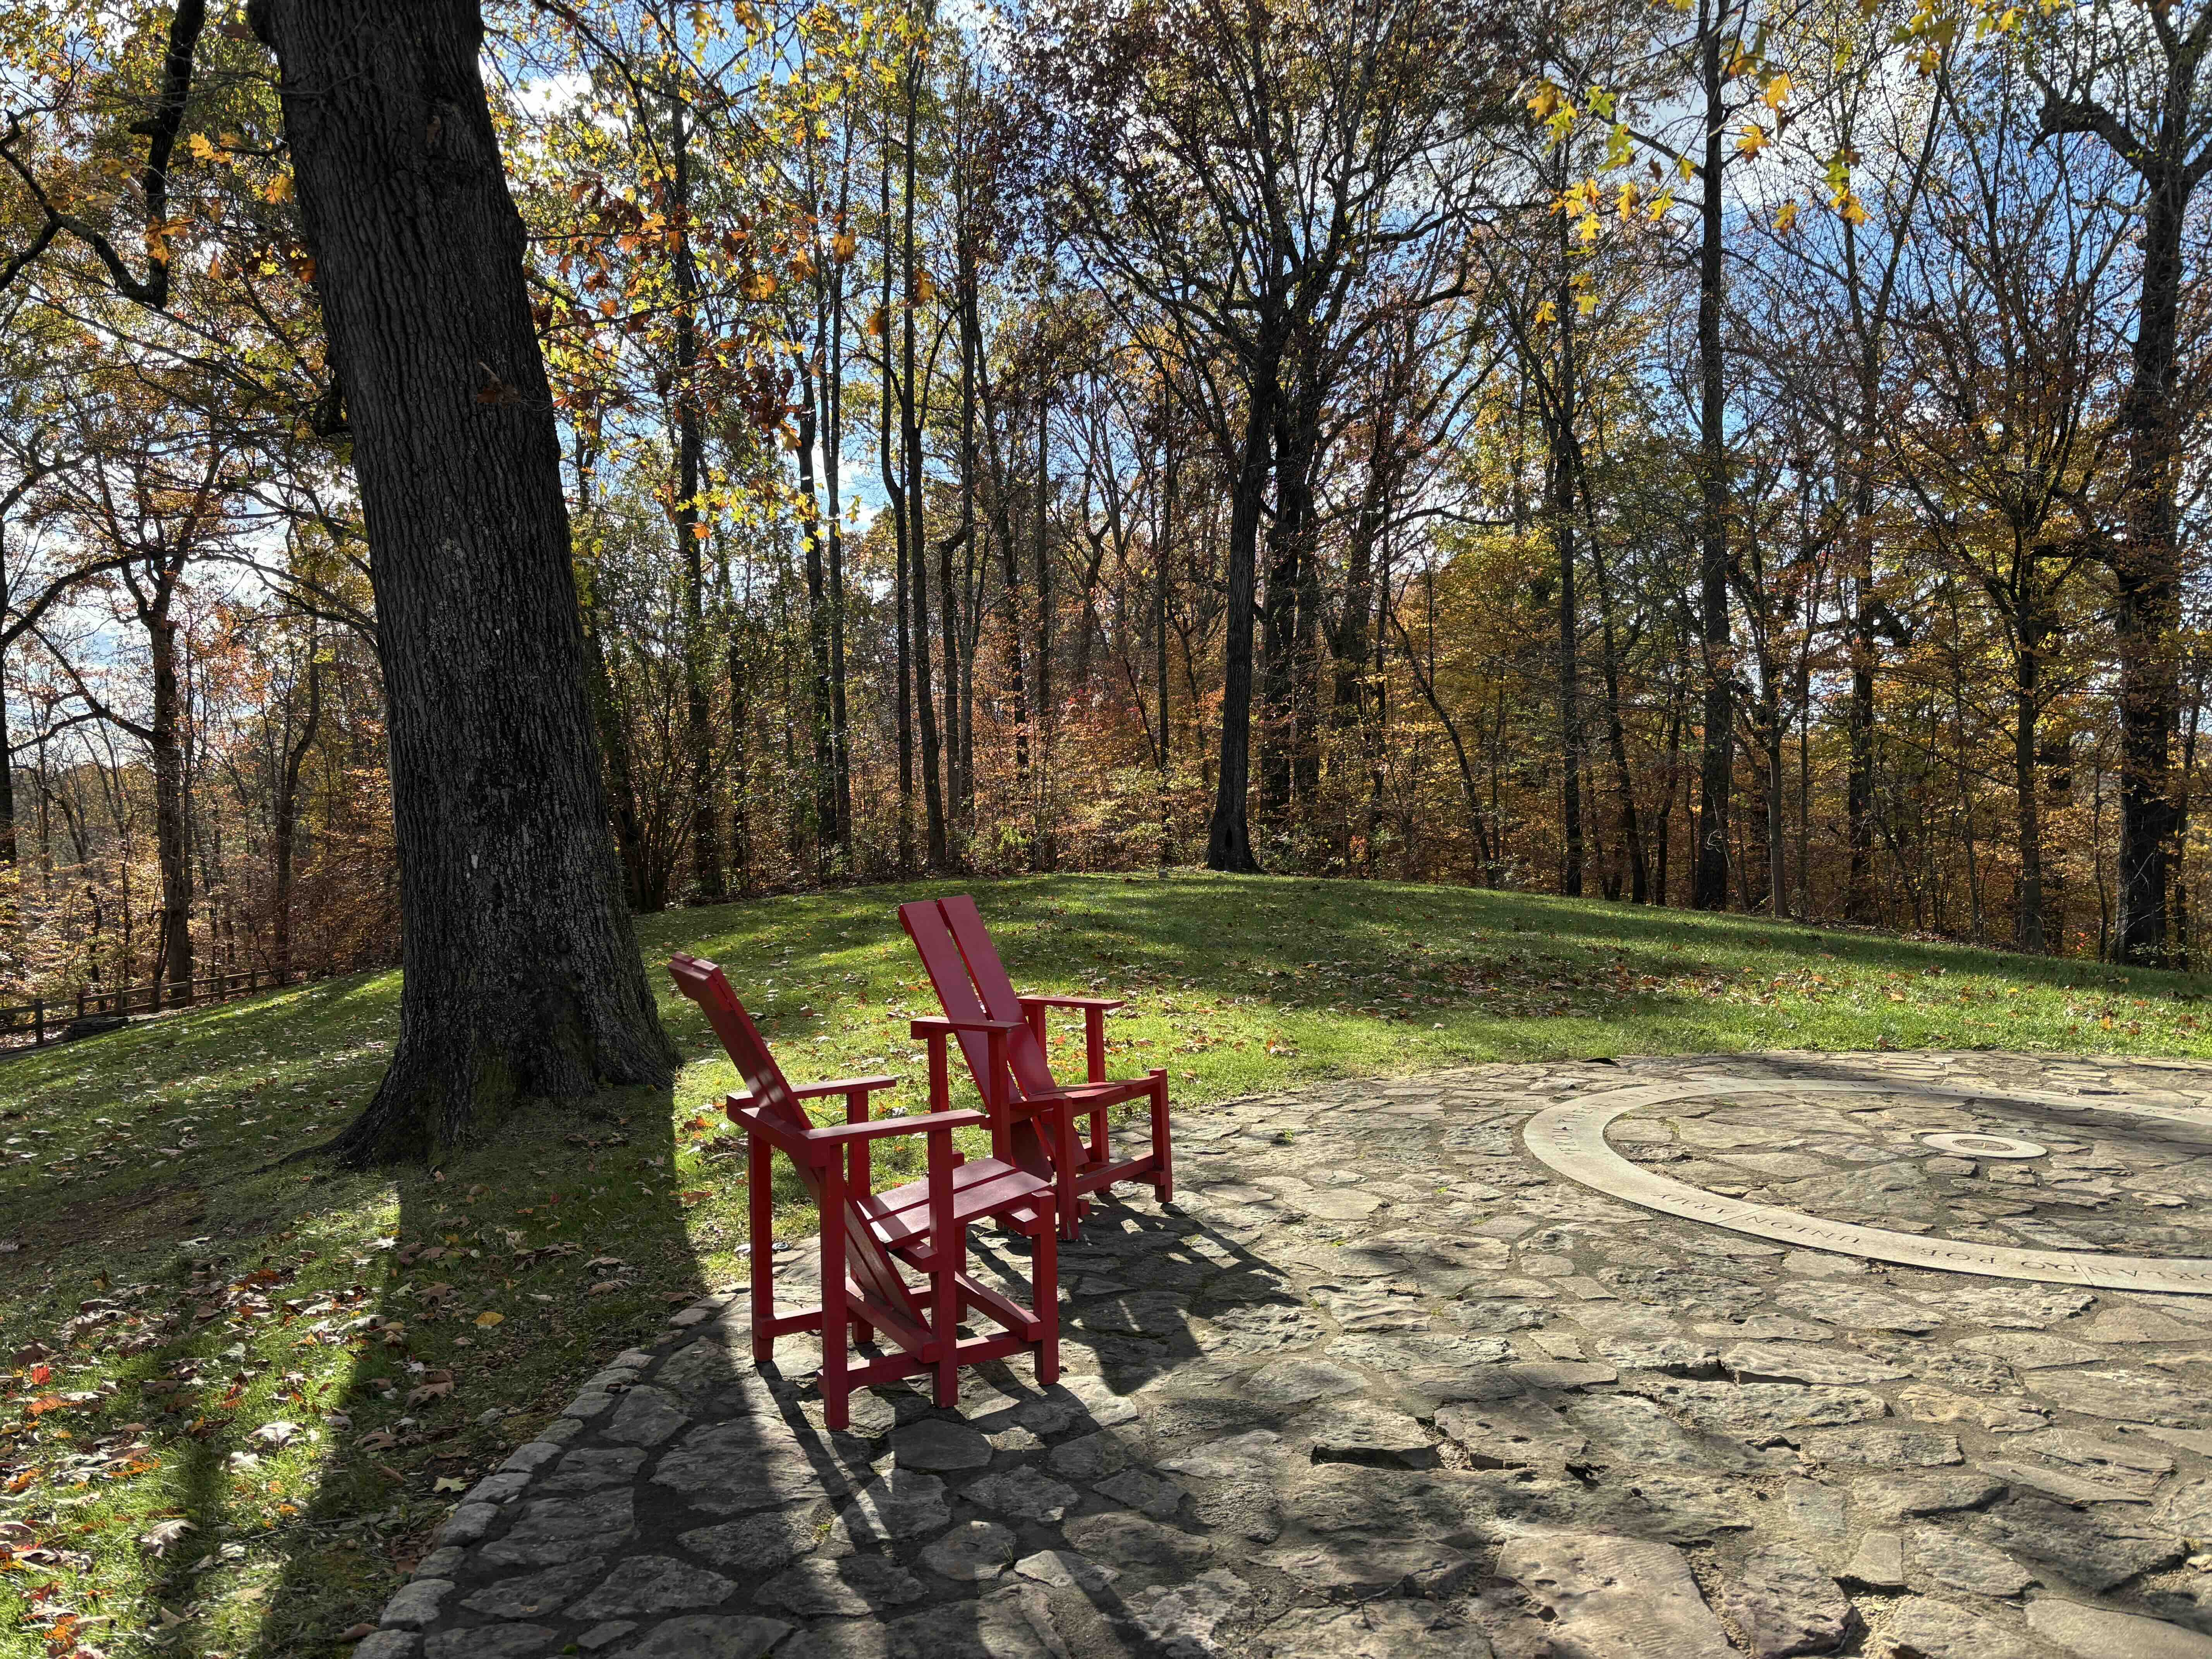
\includegraphics{img/trail-04-figure-01.jpg}

\hypertarget{directions-to-the-trailhead-3}{%
\subsubsection{Directions to the
Trailhead}\label{directions-to-the-trailhead-3}}

\begin{longtable}[]{@{}
  >{\raggedright\arraybackslash}p{(\columnwidth - 2\tabcolsep) * \real{0.5000}}
  >{\raggedright\arraybackslash}p{(\columnwidth - 2\tabcolsep) * \real{0.5000}}@{}}
\toprule\noalign{}
\begin{minipage}[b]{\linewidth}\raggedright
Trailhead Address
\end{minipage} & \begin{minipage}[b]{\linewidth}\raggedright
High Ground Park, 1000 Cherokee Trail, Knoxville, TN 37920
\end{minipage} \\
\midrule\noalign{}
\endhead
\bottomrule\noalign{}
\endlastfoot
Trailhead GPS Coordinates & 35.93824, -83.9258 \\
\end{longtable}

The trail begins from the parking lot at the above address; look for the
paved path near the back of the parking lot. You can't miss it!

\hypertarget{trail-description-3}{%
\subsubsection{Trail Description}\label{trail-description-3}}

\begin{longtable}[]{@{}
  >{\raggedright\arraybackslash}p{(\columnwidth - 2\tabcolsep) * \real{0.5000}}
  >{\raggedright\arraybackslash}p{(\columnwidth - 2\tabcolsep) * \real{0.5000}}@{}}
\toprule\noalign{}
\begin{minipage}[b]{\linewidth}\raggedright
Distance from Start
\end{minipage} & \begin{minipage}[b]{\linewidth}\raggedright
Description
\end{minipage} \\
\midrule\noalign{}
\endhead
\bottomrule\noalign{}
\endlastfoot
0 & Start off on the trail with a gentle descent. \\
0.1 & Enter the wooded part of the hike and begin a gentle climb. \\
0.35 & Red chairs and the large open area. Head toward the mowed grassy
section (followed by gravel). Alternatively, particularly if in a
stroller, return on the paved pathway you took. \\
0.4 & Look for a spur trail that heads to the site of the Fort Higley
earthworks, constructed during the Civil War by Union forces. \\
0.7 & Traihead. \\
\end{longtable}

\hypertarget{nearby-3}{%
\subsubsection{Nearby}\label{nearby-3}}

\begin{itemize}
\tightlist
\item
  Stop by a fun food hall. The nearby Kern's Food Hall (2201 Kerns
  Rising Way, Knoxville, TN 37920) has a good range of options --- and
  an outdoor play area for kids to romp around.
\item
  Hiking the nearby River Bluff Wildlife area. The nearby River Bluff
  Wildlife Area is an interesting counterbalance to the ease of High
  Ground Park - it features a short but rustic hike to a pretty overlook
  of the city. Visit Knoxville's website
  (\url{https://www.visitknoxville.com/}) has more information and a
  nice map.
\end{itemize}

\hypertarget{trail-5-ut-arboretum}{%
\subsection{Trail 5: UT Arboretum}\label{trail-5-ut-arboretum}}

\hypertarget{key-characteristics-4}{%
\subsubsection{Key Characteristics}\label{key-characteristics-4}}

\begin{longtable}[]{@{}ll@{}}
\toprule\noalign{}
Trail Name & University of Tennessee Arboretum \\
\midrule\noalign{}
\endhead
\bottomrule\noalign{}
\endlastfoot
Region & Knoxville and Surroundings \\
Trail \# & 5 \\
Time Estimate - Hiking Fast & 0.5 hours \\
Time Estimate - Hiking Slowly & 1 hour \\
Trail Distance (Miles) & 0.9 \\
Elevation Change & Gentle \\
Pets & Not Allowed \\
Parking Pass/Entrance Fee & Not Required \\
Restroom(s) & No \\
Terrain & Paved \\
\end{longtable}

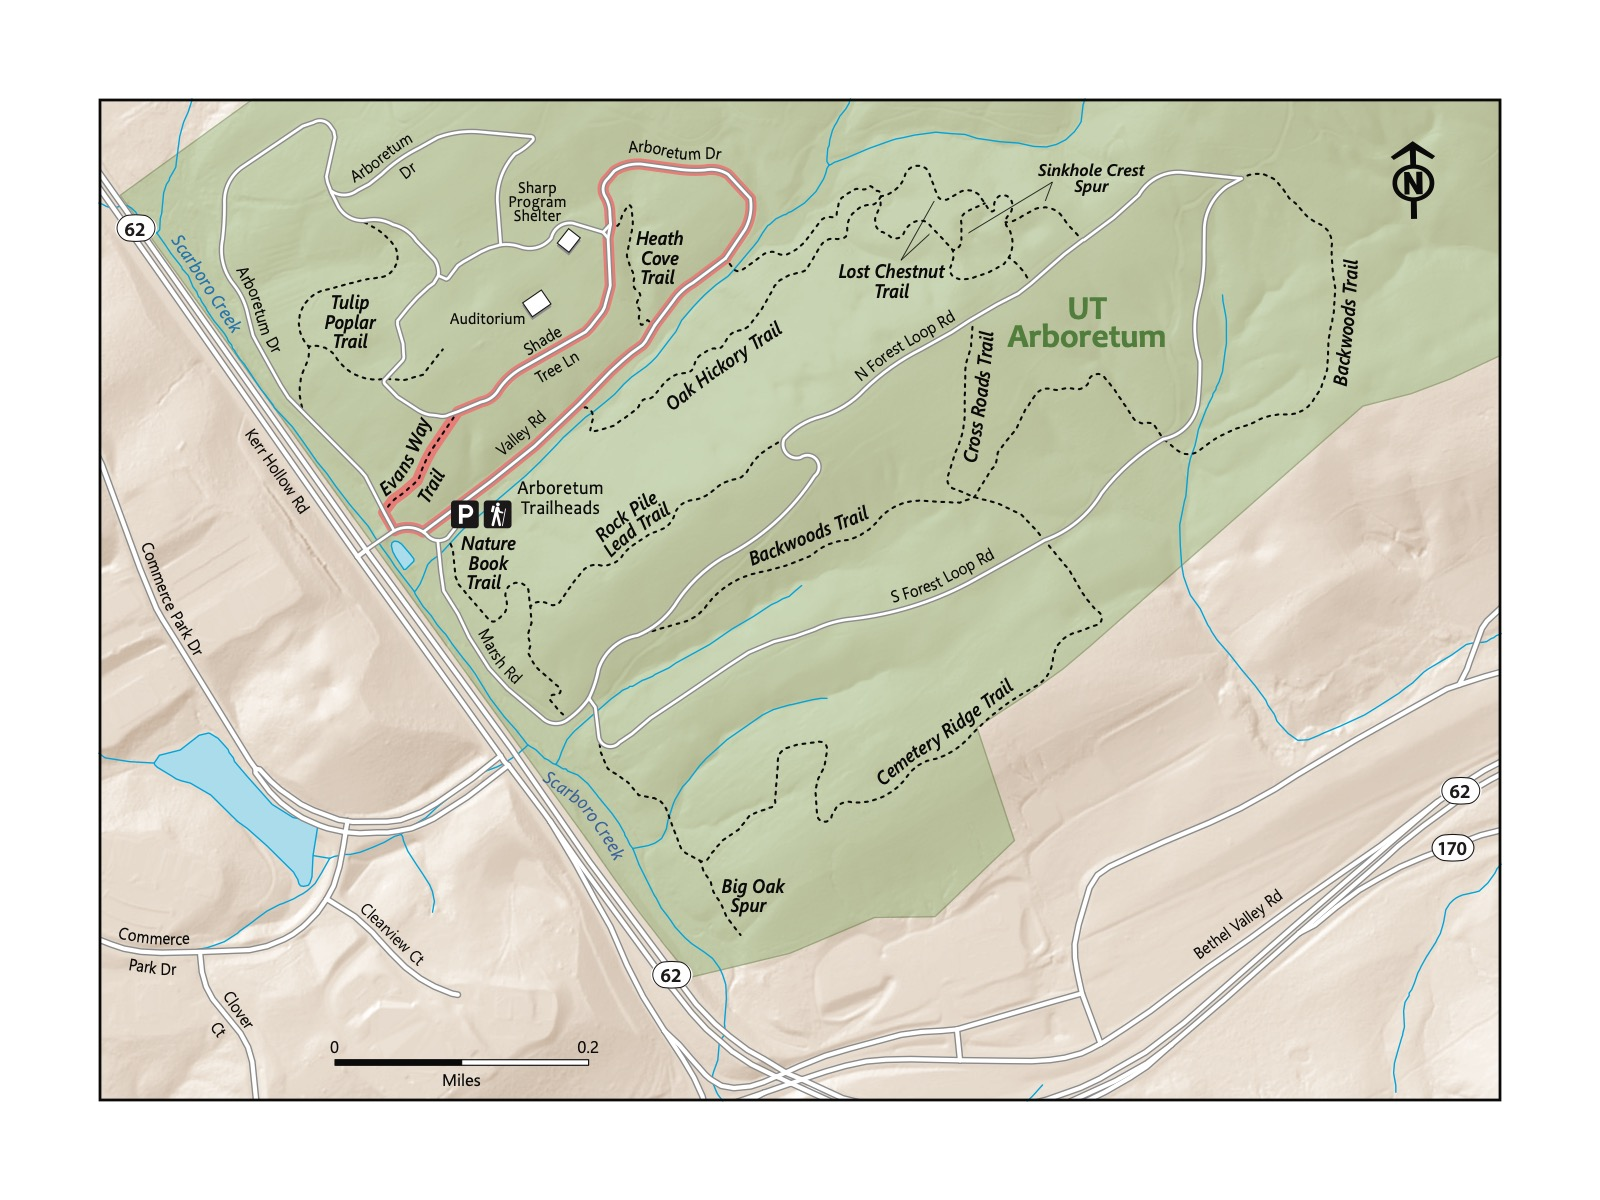
\includegraphics{maps/trail-05-map.jpeg}

\hypertarget{overview-4}{%
\subsubsection{Overview}\label{overview-4}}

A gem that is off the radar of many in Knoxville. Starts at a trailhead
with trails heading in many directions. Walk up the paved path past
botanical specimens--including unusual conifers! Circles around park
facilities past a pretty field and forests. Upon returning to the start,
there are other trails to the different ecological zones represented in
an area that is worth a visit; we like the trails near the marshy area
with the surprising, clear creek, perfect for splashing in warm weather.
Suitable for kids of all ages.

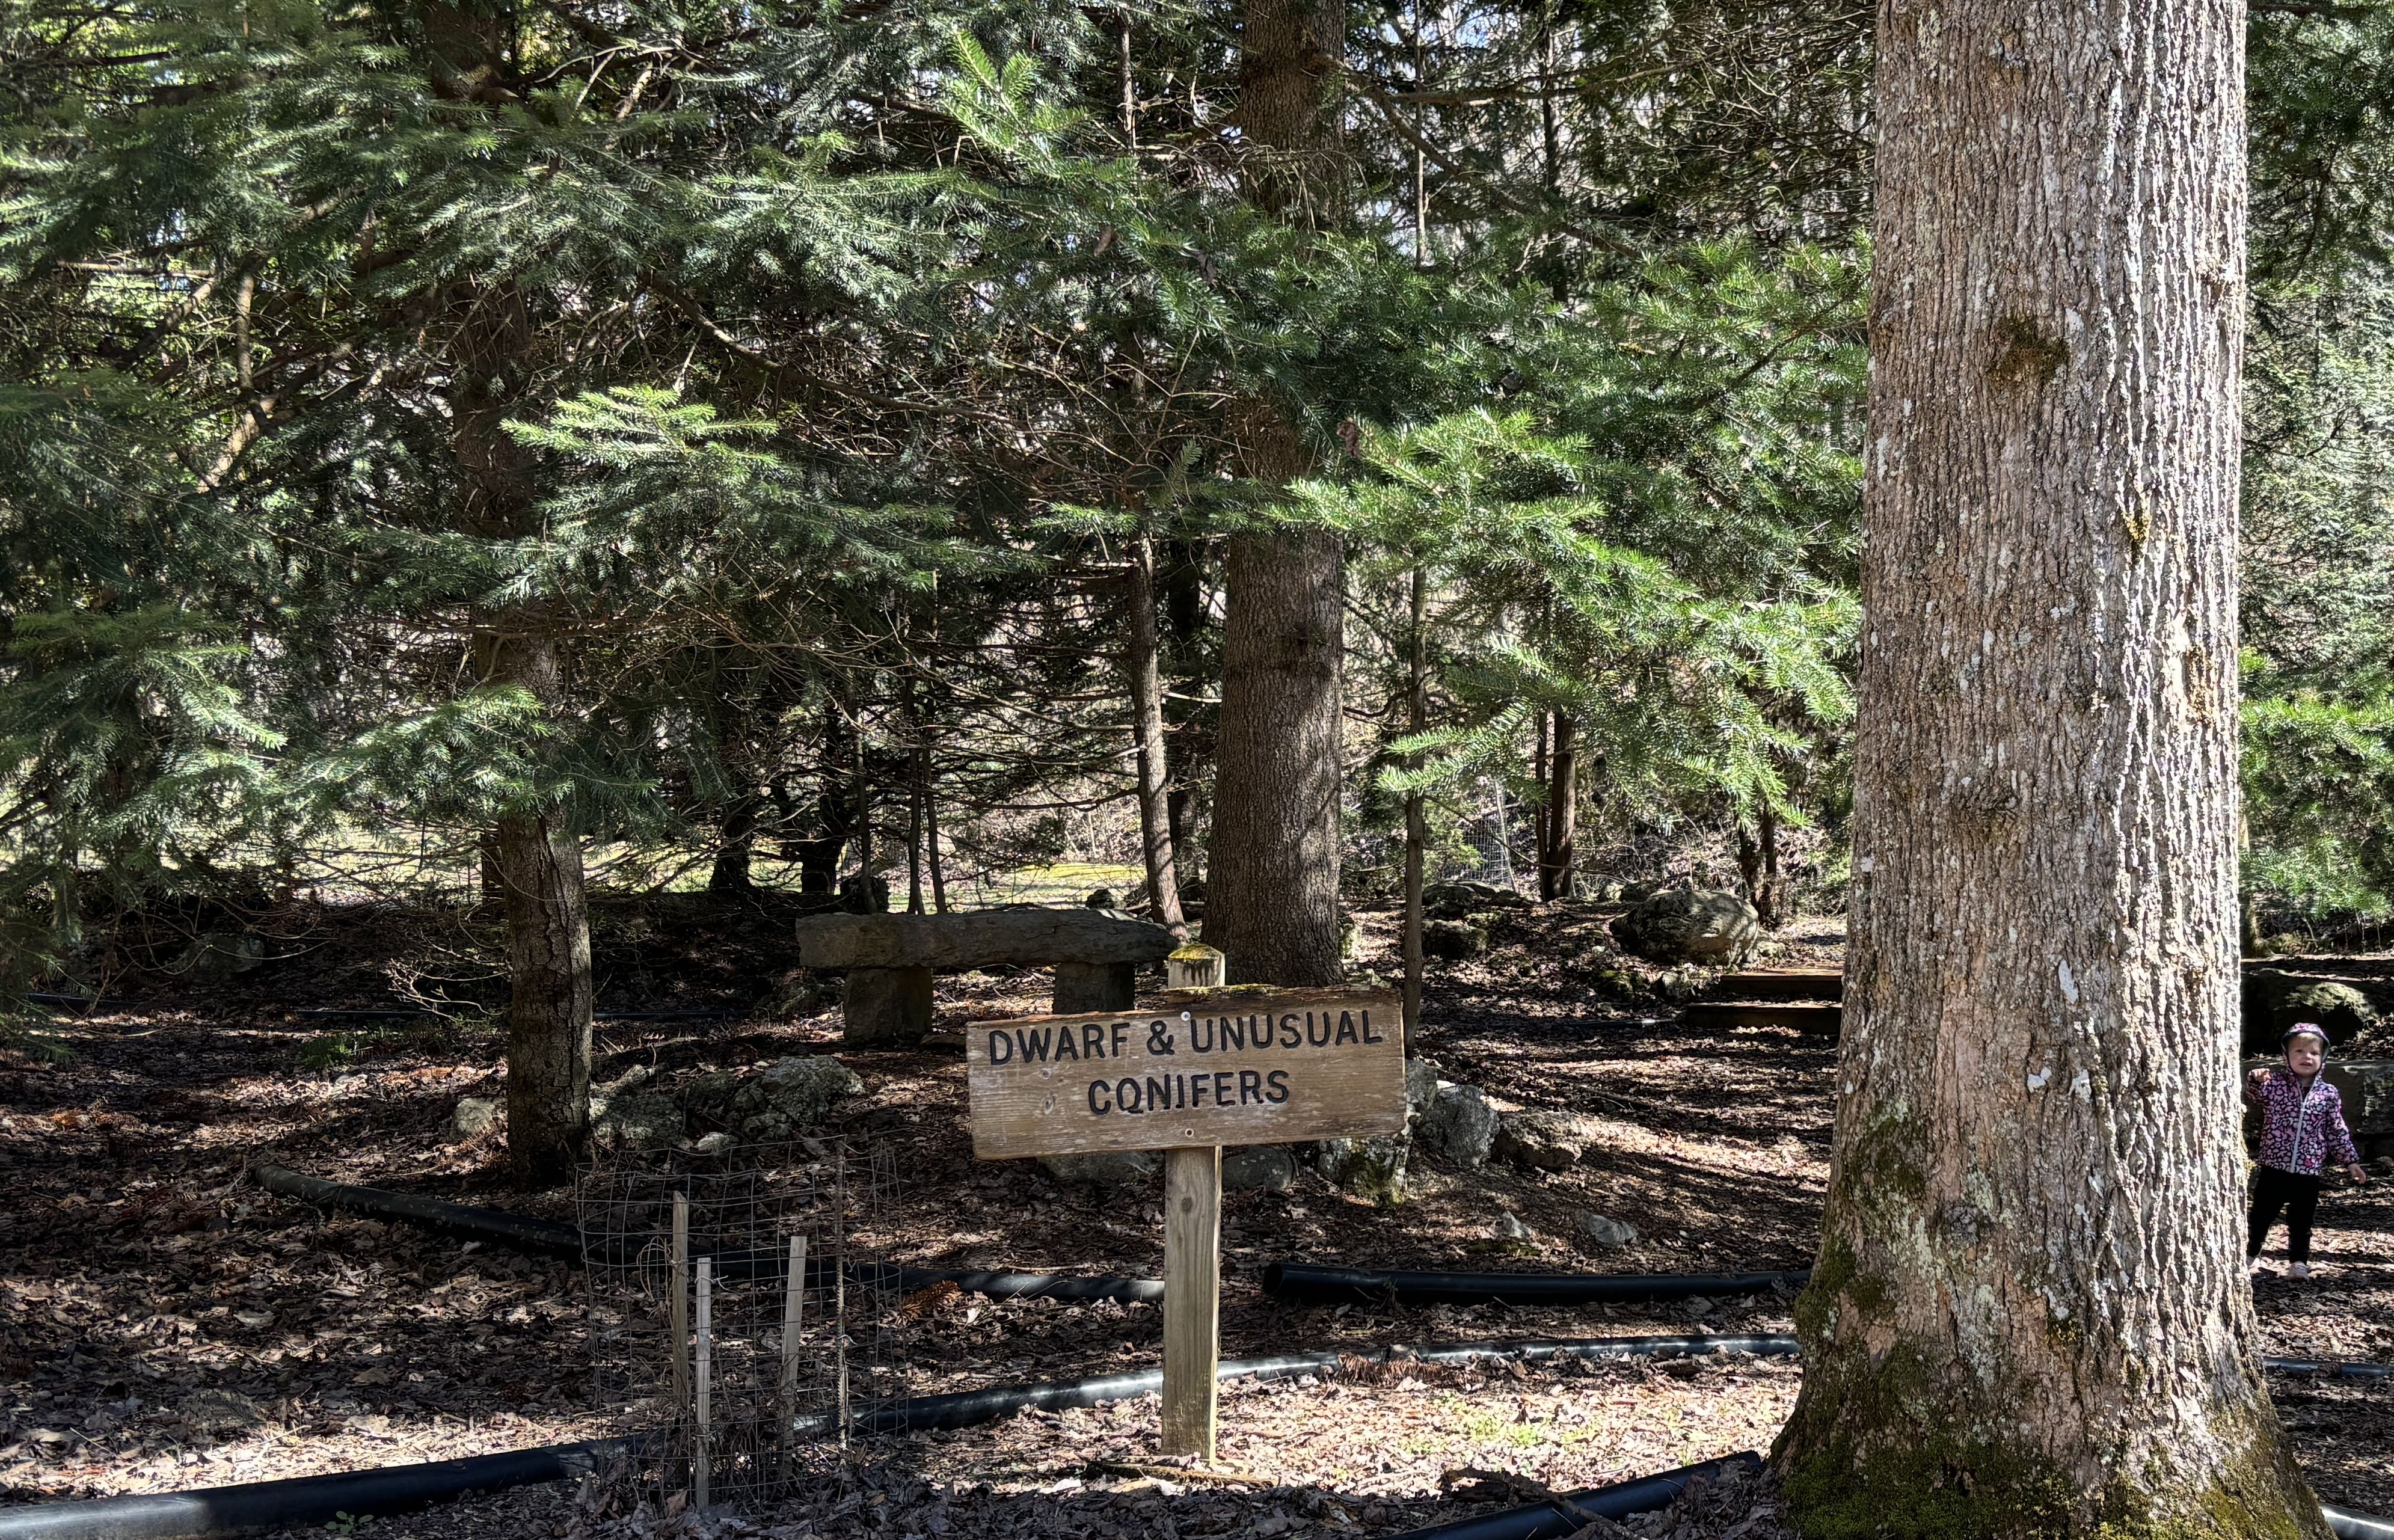
\includegraphics{img/trail-05-figure-01.jpg}

\hypertarget{directions-to-the-trailhead-4}{%
\subsubsection{Directions to the
Trailhead}\label{directions-to-the-trailhead-4}}

\begin{longtable}[]{@{}
  >{\raggedright\arraybackslash}p{(\columnwidth - 2\tabcolsep) * \real{0.5000}}
  >{\raggedright\arraybackslash}p{(\columnwidth - 2\tabcolsep) * \real{0.5000}}@{}}
\toprule\noalign{}
\begin{minipage}[b]{\linewidth}\raggedright
Trailhead Address
\end{minipage} & \begin{minipage}[b]{\linewidth}\raggedright
University of Tennessee Arboretum, 901 S Illinois Ave, Oak Ridge, TN
37830
\end{minipage} \\
\midrule\noalign{}
\endhead
\bottomrule\noalign{}
\endlastfoot
Trailhead GPS Coordinates & 35.99392, -84.21988 \\
\end{longtable}

The trailhead is easy to find with the above address. Park in the large
parking lot for the University of Tennessee Arboretum look for the road
connected to it, and headed straight away from the parking area. The
small stop sign that says ``Authorized Vehicles Only'' is at the start
of this hike.

\hypertarget{trail-description-4}{%
\subsubsection{Trail Description}\label{trail-description-4}}

\begin{longtable}[]{@{}
  >{\raggedright\arraybackslash}p{(\columnwidth - 2\tabcolsep) * \real{0.5000}}
  >{\raggedright\arraybackslash}p{(\columnwidth - 2\tabcolsep) * \real{0.5000}}@{}}
\toprule\noalign{}
\begin{minipage}[b]{\linewidth}\raggedright
Distance from Start
\end{minipage} & \begin{minipage}[b]{\linewidth}\raggedright
Description
\end{minipage} \\
\midrule\noalign{}
\endhead
\bottomrule\noalign{}
\endlastfoot
0.0 & Walk along the paved road. \\
0.1 & Start of the Oak-Hickory Trail on the right. \\
0.2 & Start of the Heath Cove Trail on the left. This is a shortcut if
you're looking for one! \\
0.3 & Wind around, still on the road. \\
0.5 & Shelter on the right. \\
0.6 & Auditorium on the right. \\
0.7 & Leave the paved road for a short dirt path called Evans Way Trail.
Alternatively, turn around and head back on the paved path (or continue
along many nearby trails! \\
0.9 & Traihead. \\
\end{longtable}

\includegraphics{img/trail-05-figure-02.jpg}

\hypertarget{nearby-4}{%
\subsubsection{Nearby}\label{nearby-4}}

\begin{itemize}
\tightlist
\item
  Exploring the many other trails nearby. The trail we featured meanders
  through a very small section of a large, diverse park. The Nature Book
  Trail is a great trail to add on to your hike. There are many others;
  check out the map at the UT Arboretum website
  (\url{https://utarboretum.tennessee.edu/}) to learn more.
\item
  Stopping by Haw Ridge and its kids' pump track. Nearby Haw Ridge Park
  features the Dirtlab Mountain Bike Skill Park, a great spot for kids
  riding strider and pedal bikes to hone their skills and build
  confidence.
\end{itemize}

\hypertarget{trail-6-knox-blount-greenway}{%
\subsection{Trail 6: Knox-Blount
Greenway}\label{trail-6-knox-blount-greenway}}

\hypertarget{key-characteristics-5}{%
\subsubsection{Key Characteristics}\label{key-characteristics-5}}

\begin{longtable}[]{@{}ll@{}}
\toprule\noalign{}
Trail Name & Knox-Blount Greenway \\
\midrule\noalign{}
\endhead
\bottomrule\noalign{}
\endlastfoot
Region & Knoxville and Surroundings \\
Trail \# & 6 \\
Time Estimate - Hiking Fast & 45 minutes \\
Time Estimate - Hiking Slowly & 1.5 hours \\
Trail Distance (Miles) & 2.3 \\
Elevation Change & Gentle \\
Pets & Allowed on leash \\
Parking Pass/Entrance Fee & Not Required \\
Restroom(s) & No \\
Terrain & Paved \\
\end{longtable}

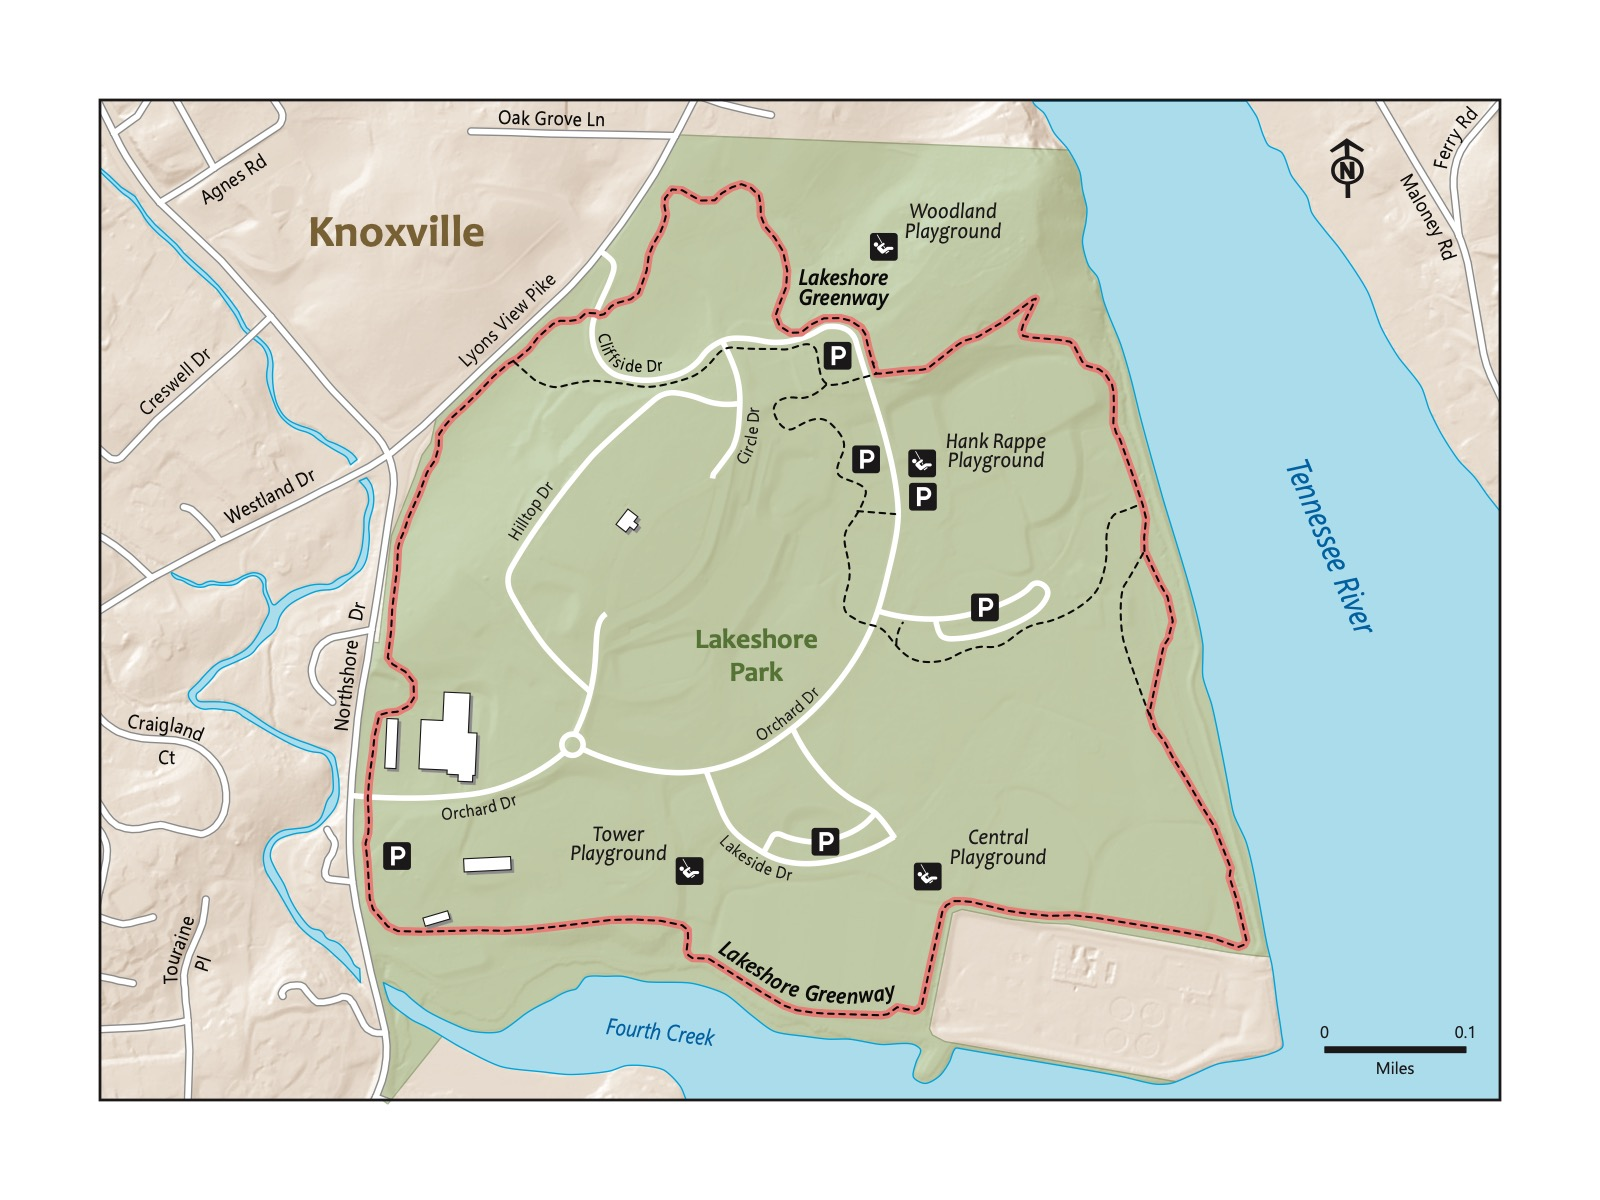
\includegraphics{maps/trail-03-map.jpeg}

\hypertarget{overview-5}{%
\subsubsection{Overview}\label{overview-5}}

Another hike that is very close to city center Knoxville, the
Knox-Blount Greenway is a fun, easier outing for little walkers and for
parents pushing little ones in strollers. Paved throughout, this trail
offers a glimpse of the surprising beauty of the Tennessee River so
close to the city. Our description features a route that heads to the
north, toward the city, and then back to the trail from the research
park further south before returning to the start; of course, you can
hike any way you like! Look for blue herons and other birds along the
side of the river; you might see a Bald Eagle! Limited shade makes this
a great outing for clear but cold winter days but a hot hike during
warmer, sunnier times. This will be a fun hike for a gaggle of kids
looking to toddle or run wild!

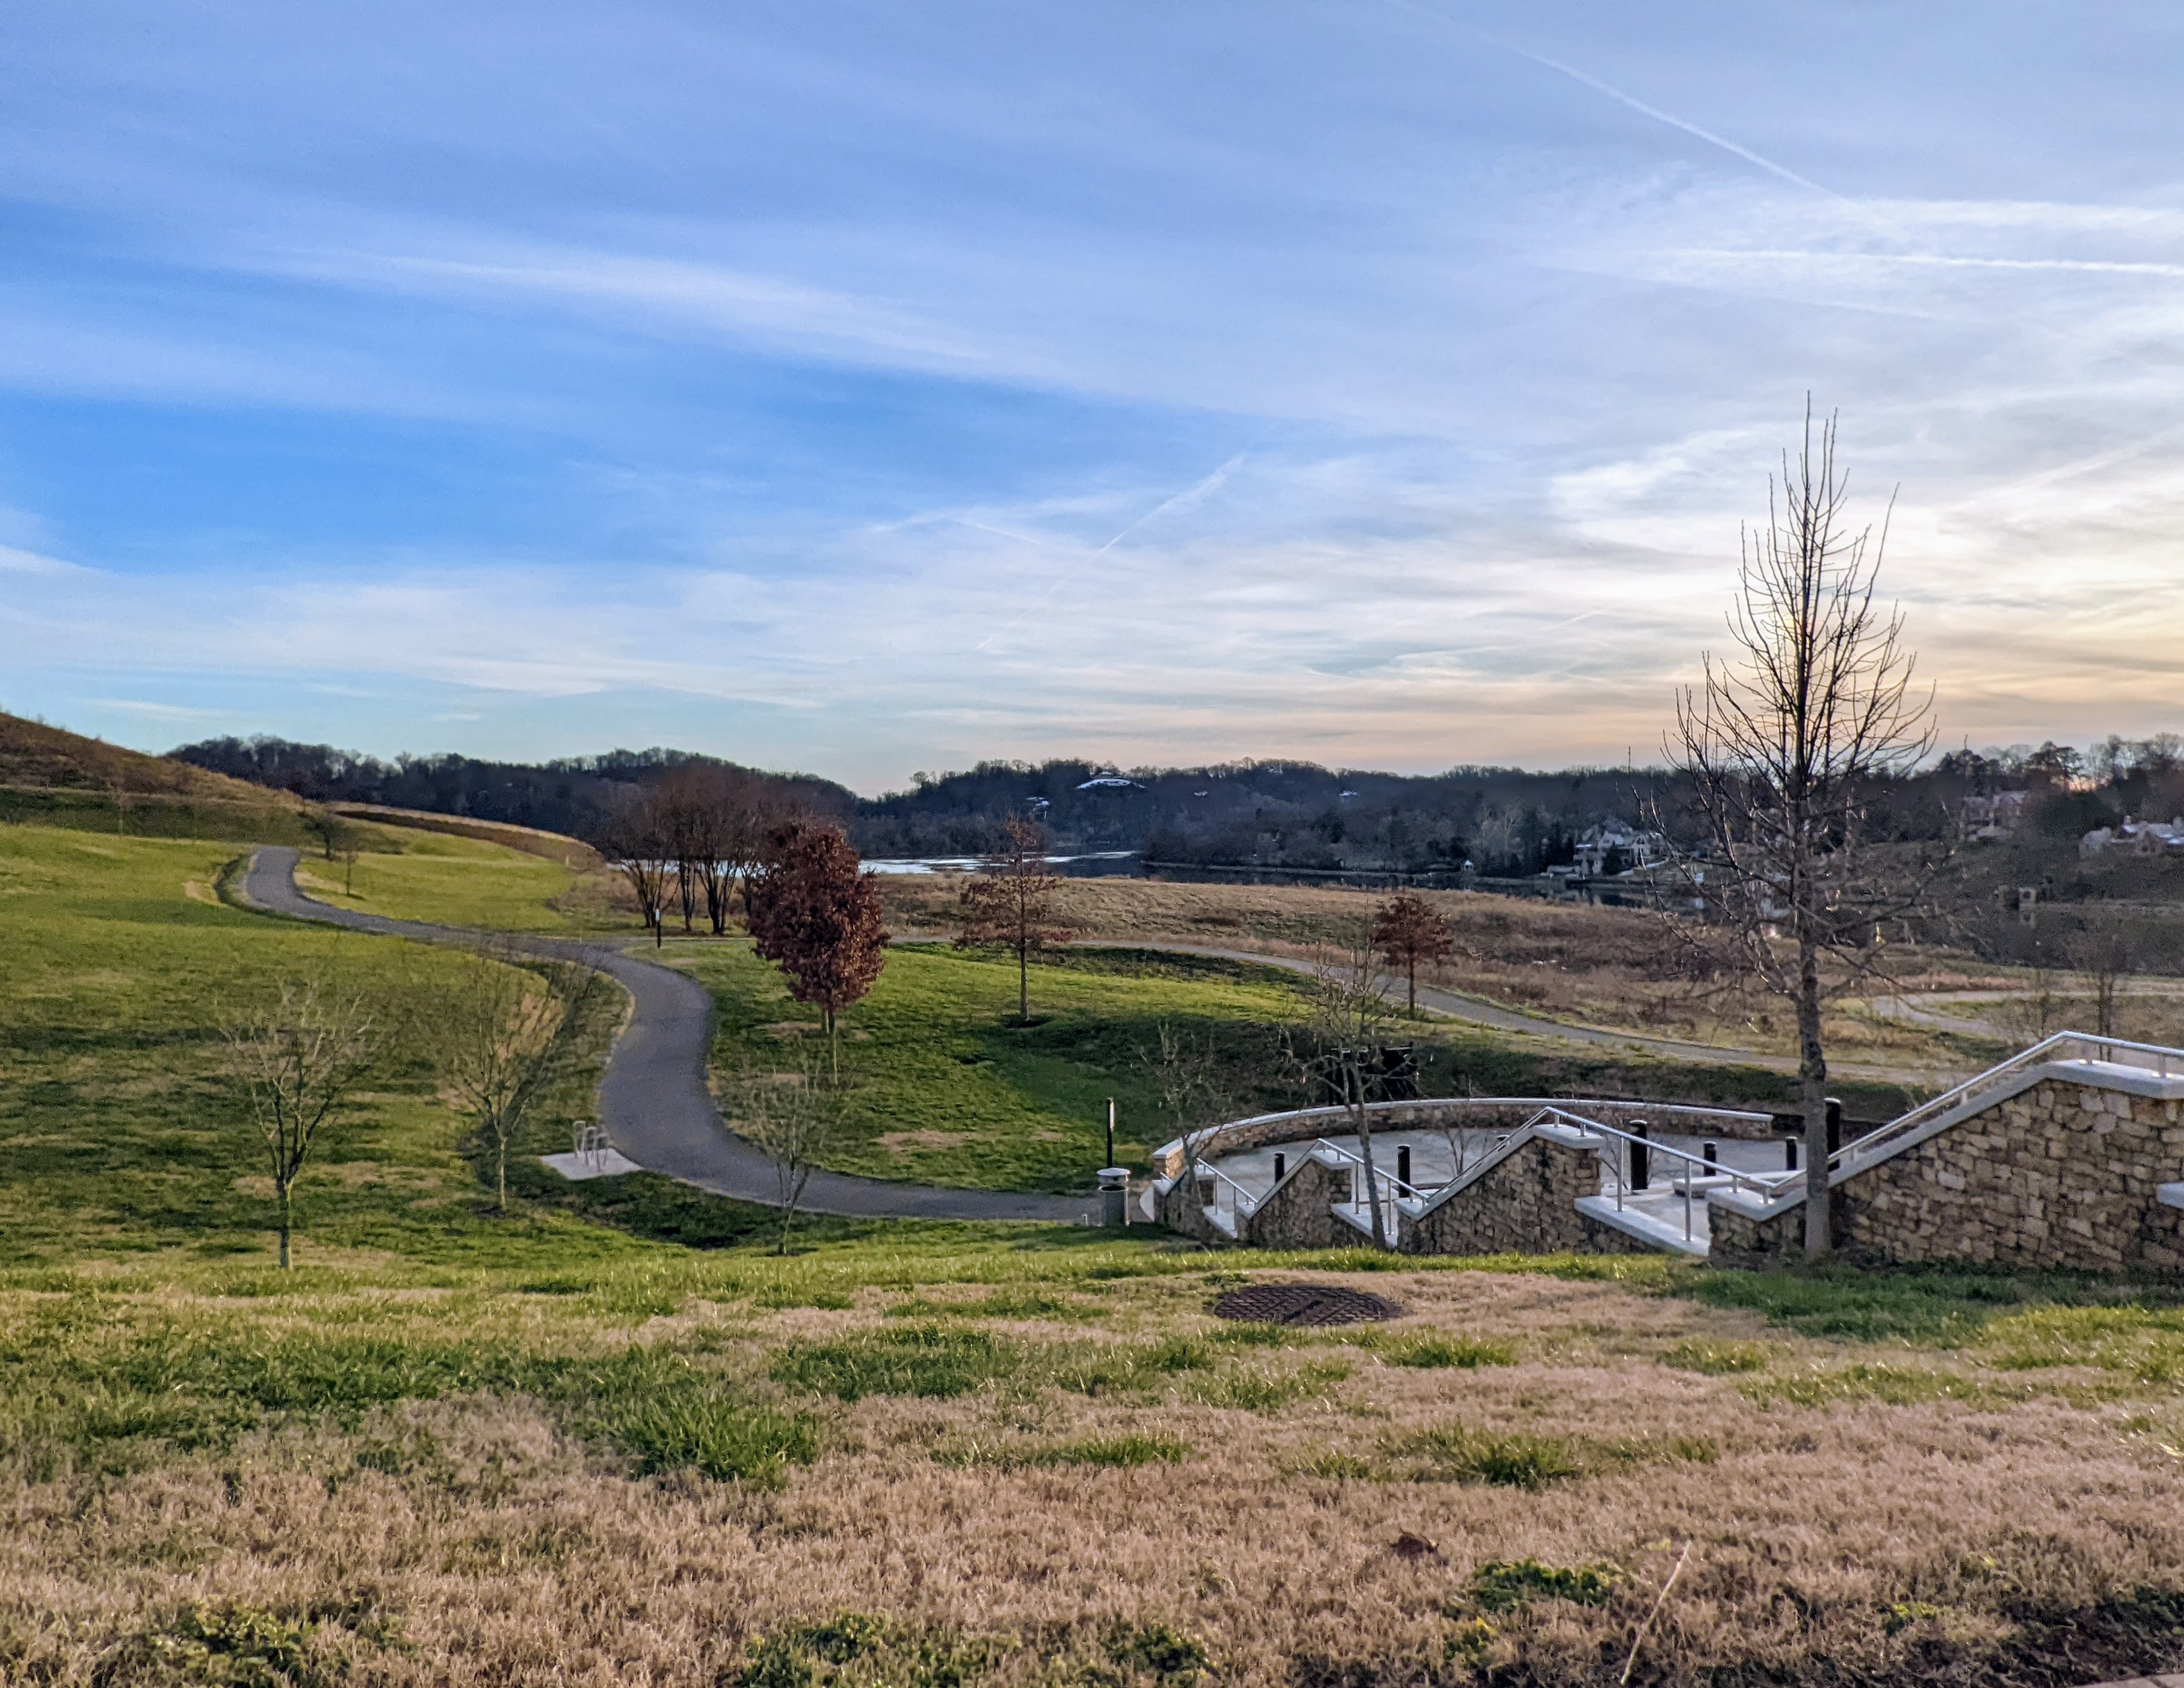
\includegraphics{img/trail-06-figure-01.jpg}

\hypertarget{directions-to-the-trailhead-5}{%
\subsubsection{Directions to the
Trailhead}\label{directions-to-the-trailhead-5}}

\begin{longtable}[]{@{}
  >{\raggedright\arraybackslash}p{(\columnwidth - 2\tabcolsep) * \real{0.5000}}
  >{\raggedright\arraybackslash}p{(\columnwidth - 2\tabcolsep) * \real{0.5000}}@{}}
\toprule\noalign{}
\begin{minipage}[b]{\linewidth}\raggedright
Trailhead Address
\end{minipage} & \begin{minipage}[b]{\linewidth}\raggedright
University of Tennessee Research Park at Cherokee Farm, 2641 Osprey
Vista Way, Knoxville, TN 37920
\end{minipage} \\
\midrule\noalign{}
\endhead
\bottomrule\noalign{}
\endlastfoot
Trailhead GPS Coordinates & 35.94191, -83.95270 \\
\end{longtable}

Park in the lot at the above address---if helpful, the building is the
``IAM Electron Microscopy Facility''! The start of the trail is at the
top of a terraced amphitheater --- conveniently, one that's easy to walk
down.

\hypertarget{trail-description-5}{%
\subsubsection{Trail Description}\label{trail-description-5}}

\begin{longtable}[]{@{}
  >{\raggedright\arraybackslash}p{(\columnwidth - 2\tabcolsep) * \real{0.5000}}
  >{\raggedright\arraybackslash}p{(\columnwidth - 2\tabcolsep) * \real{0.5000}}@{}}
\toprule\noalign{}
\begin{minipage}[b]{\linewidth}\raggedright
Distance from Start
\end{minipage} & \begin{minipage}[b]{\linewidth}\raggedright
Description
\end{minipage} \\
\midrule\noalign{}
\endhead
\bottomrule\noalign{}
\endlastfoot
0.0 & Walk down the terraced amphitheater. \\
0.1 & Begin to descend down a gradual hill. \\
0.3 & Reach the river and the Knox-Blount Greenway trail proper. Our
route turns right, but you can explore in either direction! \\
0.35 & Follow the greenway along the river. The meadows to the right are
usually mowed; kids may like to cruise through them! \\
0.8 & Our preferred route turns around at the intersection of the
greenway and a spur trail. Of course, you can continue further if you
like. Head back the other direction \\
1.3 & Pass the trail from the amphitheater you took earlier, continuing
along the river. \\
1.65 & Turn around at the intersection of another spur trail---or,
again, continue further. \\
2.0 & Meet back up with the trail to the amphitheater. \\
2.3 & Traihead. \\
\end{longtable}

\hypertarget{nearby-5}{%
\subsubsection{Nearby}\label{nearby-5}}

\begin{itemize}
\tightlist
\item
  Visiting the UT Gardens. The nearby UT Gardens (2621 Morgan Circle,
  Knoxville, TN 37996) is a great spot for a meander through beautiful
  gardens. Be sure to check out the Children's Garden featuring grassy
  moguls kids love to roll or hop down.
\item
  Biking the greenways. While we featured the Knox-Blount Greenway as a
  hike, it's also a fun bike ride for young bikers.
\end{itemize}

\hypertarget{trail-7-sequoyah-park}{%
\subsection{Trail 7: Sequoyah Park}\label{trail-7-sequoyah-park}}

\hypertarget{key-characteristics-6}{%
\subsubsection{Key Characteristics}\label{key-characteristics-6}}

\begin{longtable}[]{@{}ll@{}}
\toprule\noalign{}
Trail Name & Sequoyah Park \\
\midrule\noalign{}
\endhead
\bottomrule\noalign{}
\endlastfoot
Region & Knoxville and Surroundings \\
Trail \# & 7 \\
Time Estimate - Hiking Fast & 1 hour \\
Time Estimate - Hiking Slowly & 2 hours \\
Trail Distance (Miles) & 2.1 \\
Elevation Change & Flat \\
Pets & Allowed on leash \\
Parking Pass/Entrance Fee & Not Required \\
Restroom(s) & Yes \\
Terrain & Dirt path; grass; gravel path \\
\end{longtable}

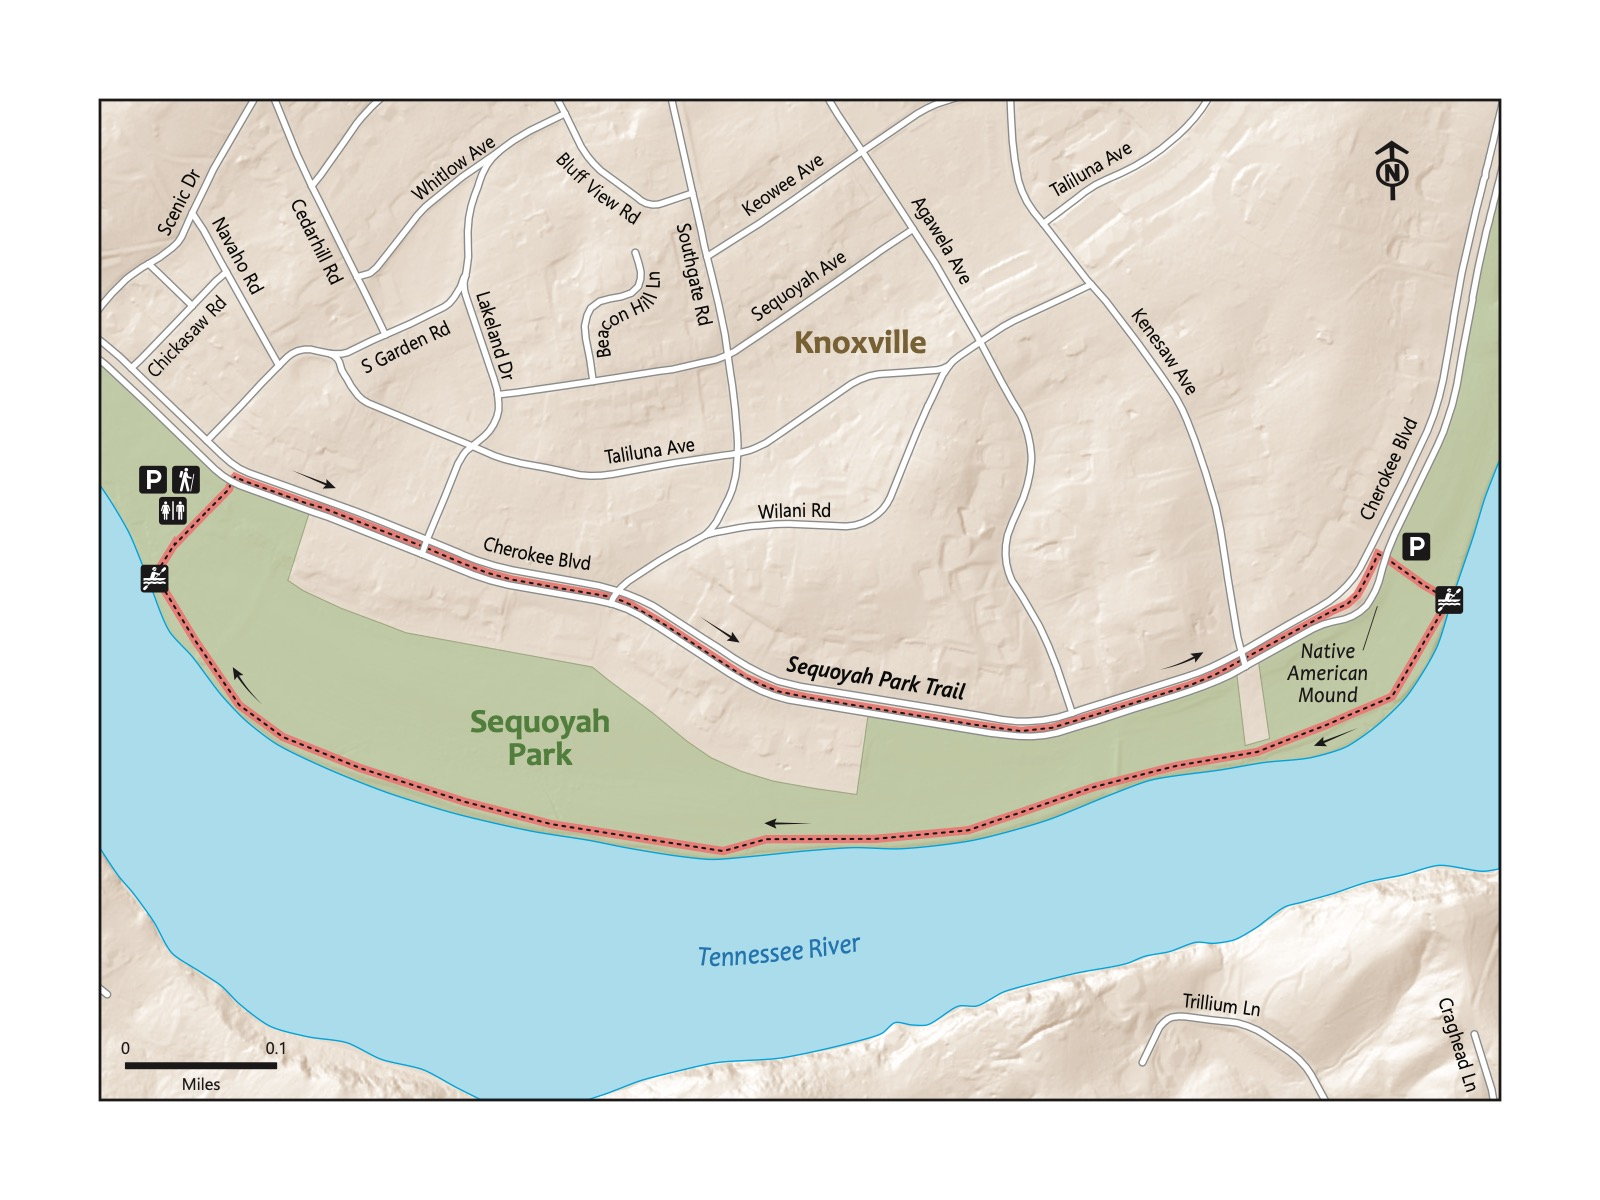
\includegraphics{maps/trail-07-map.jpeg}

\hypertarget{overview-6}{%
\subsubsection{Overview}\label{overview-6}}

Another gem among Knoxville city parks. The trail starts at a large
parking area near the restroom building and walks towards the river. It
follows the river past open fields, trees, and bushes that are
practically impossible for kids not to explore. The trail cuts up toward
the greenway and hikes past Indian burial mounds and the old (many
large) houses along the path before returning to the start. In mild
weather, it is a fantastic spot to hang up a hammock, go fish, have a
picnic, or toss a frisbee or a football. Good for kids of all walking
ages; alternate ways to access the greenway make it easy to create a
shorter loop.

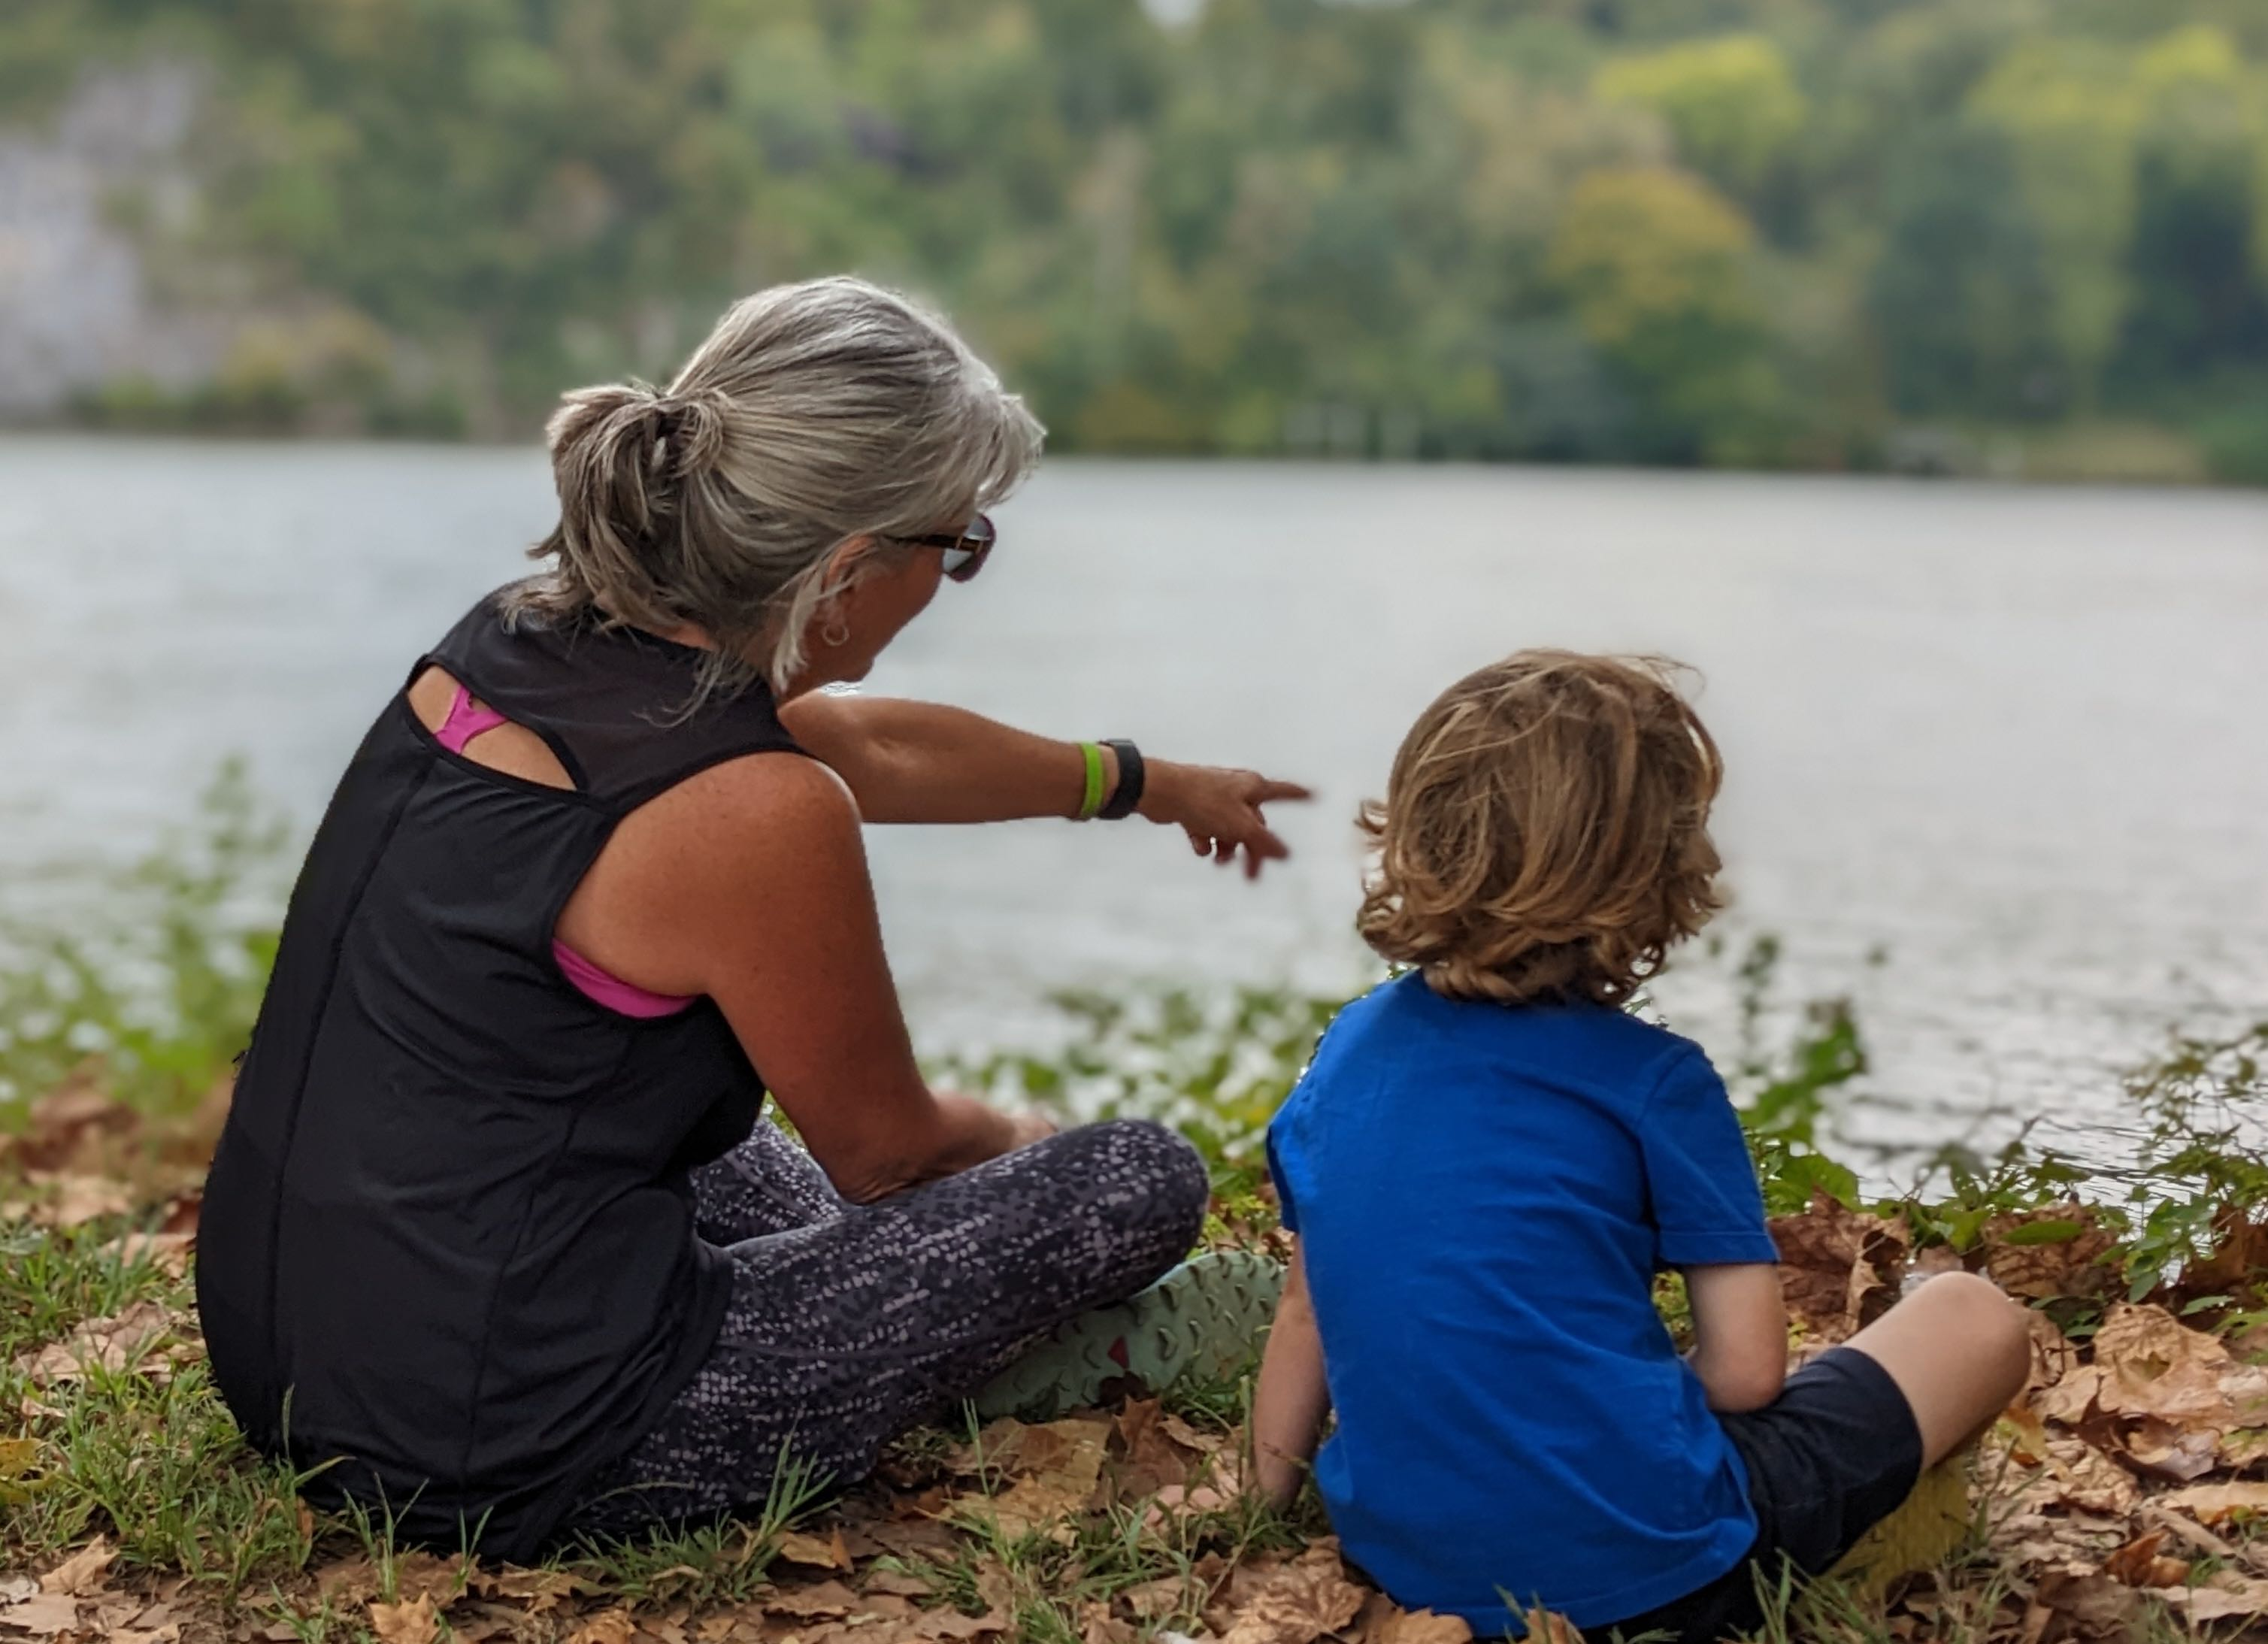
\includegraphics{img/trail-07-figure-01.jpg}

\hypertarget{directions-to-the-trailhead-6}{%
\subsubsection{Directions to the
Trailhead}\label{directions-to-the-trailhead-6}}

\begin{longtable}[]{@{}
  >{\raggedright\arraybackslash}p{(\columnwidth - 2\tabcolsep) * \real{0.5000}}
  >{\raggedright\arraybackslash}p{(\columnwidth - 2\tabcolsep) * \real{0.5000}}@{}}
\toprule\noalign{}
\begin{minipage}[b]{\linewidth}\raggedright
Trailhead Address
\end{minipage} & \begin{minipage}[b]{\linewidth}\raggedright
Sequoyah Park Restrooms, W2HG+M9, Knoxville, TN 37919
\end{minipage} \\
\midrule\noalign{}
\endhead
\bottomrule\noalign{}
\endlastfoot
Trailhead GPS Coordinates & 35.92932, -83.97398 \\
\end{longtable}

The above address takes you to the restrooms that serve as a landmark
for this sprawling park. Please note that the address uses a ``Plus''
code that only works with Google Maps because the restrooms and
trailhead don't have an assigned address.

Park in the large parking area and head toward the river and the large
Elm tree with the steel wire around it. The trail begins there along the
river.

\hypertarget{trail-description-6}{%
\subsubsection{Trail Description}\label{trail-description-6}}

\begin{longtable}[]{@{}
  >{\raggedright\arraybackslash}p{(\columnwidth - 2\tabcolsep) * \real{0.5000}}
  >{\raggedright\arraybackslash}p{(\columnwidth - 2\tabcolsep) * \real{0.5000}}@{}}
\toprule\noalign{}
\begin{minipage}[b]{\linewidth}\raggedright
Distance from Start
\end{minipage} & \begin{minipage}[b]{\linewidth}\raggedright
Description
\end{minipage} \\
\midrule\noalign{}
\endhead
\bottomrule\noalign{}
\endlastfoot
0.0 & Walk southwest (toward the large, open part of the park) along the
river. \\
0.1 & Kayak and canoe put in spot on the right. \\
0.25 & Enter a wooded section.. \\
0.4 & Bench. \\
0.65 & Distinctive, dome-shaded trees that kids can crawl into, between,
and through. \\
0.9 & Small rocky hill to walk over (you can walk around it on the
greenway, but kids may enjoy scrambling up it). \\
1.1 & Boat launch. Head up beside or through the parking lot to Sequoyak
Greenway in the center of Cherokee Blvd. Turn left onto the greenway. \\
1.2 & Indian burial mound. Note the historical marker. Walk along past
the homes on both sides of the greenway. \\
2.05 & Traihead. \\
\end{longtable}

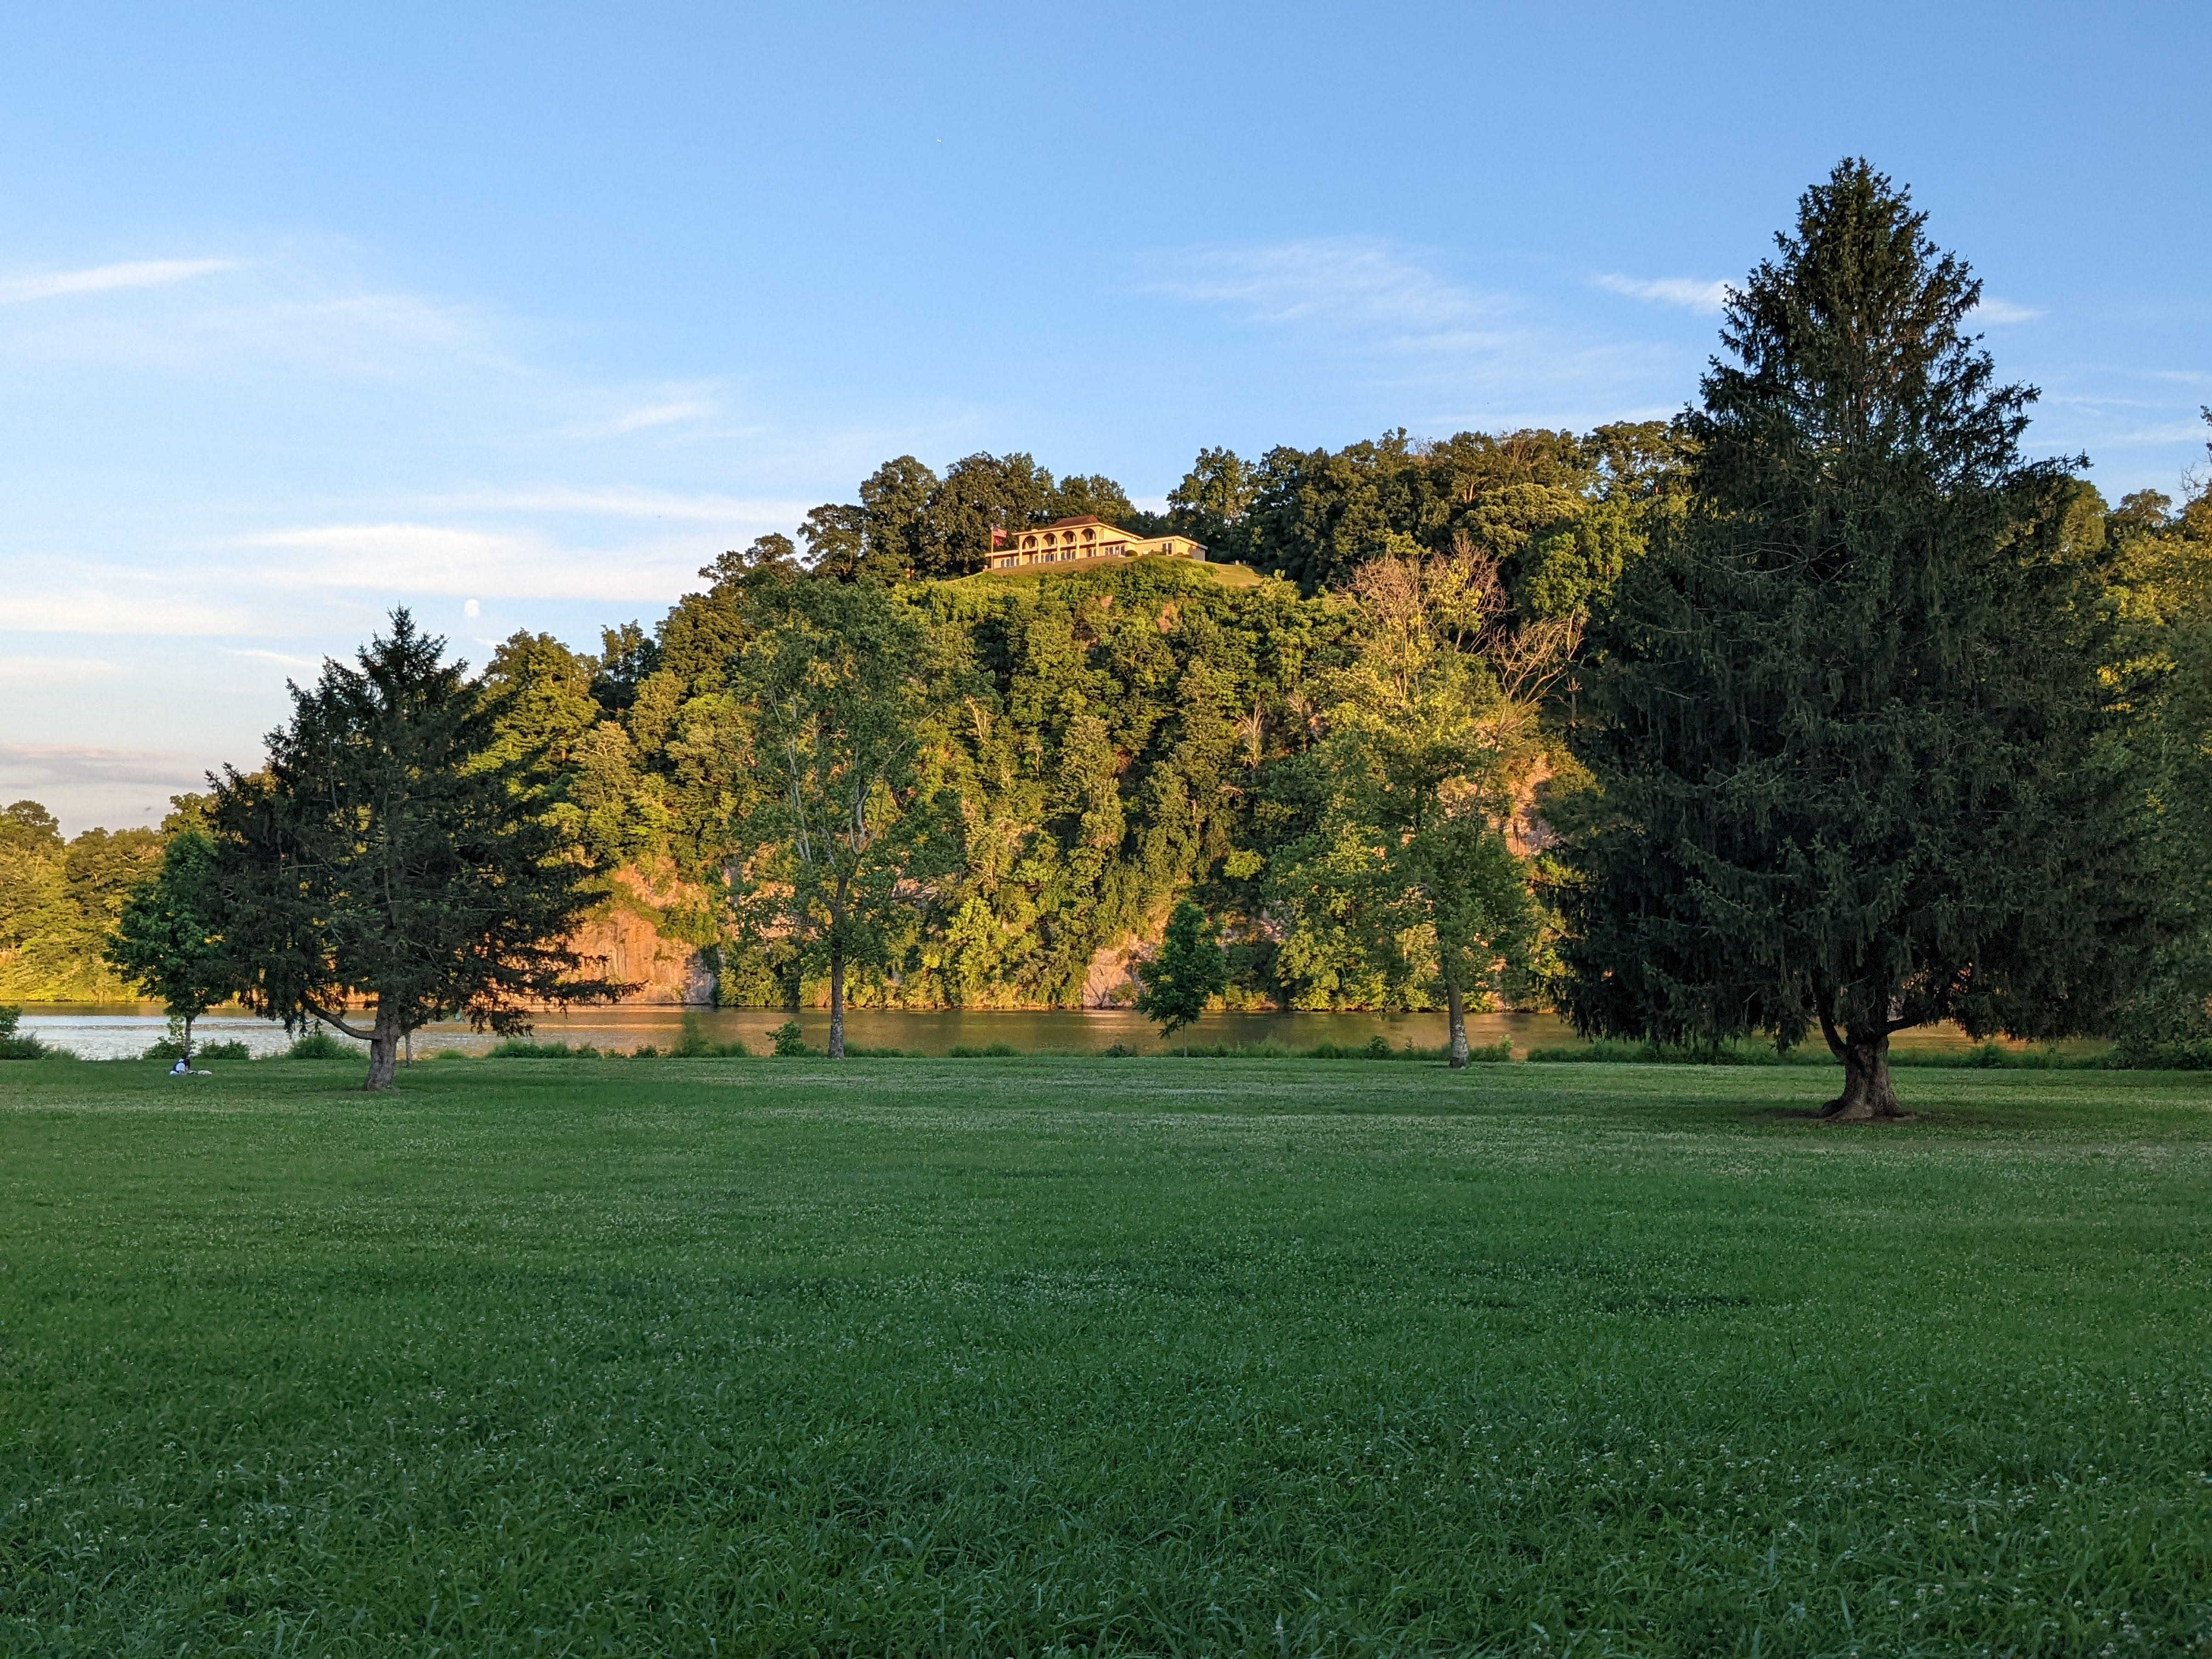
\includegraphics{img/trail-07-figure-02.jpg}

\hypertarget{nearby-6}{%
\subsubsection{Nearby}\label{nearby-6}}

\begin{itemize}
\tightlist
\item
  Grabbing a great cup of coffee --- or breakfast. Nearby Treetop Coffee
  Shop (1206 Kenesaw Ave, Knoxville, TN 37919) and The Plaid Apron
  restaurant (1210 Kenesaw Ave, Knoxville, TN 37919) next door are great
  places to stop by.
\item
  Playing at a nearby playground. Nearby Whitlow Park (4228 Whitlow Ave
  SW, Knoxville, TN 37919) features a small but fun playground, nice
  tennis courts, and a basketball court.
\end{itemize}

\hypertarget{trail-8-ijams-crag}{%
\subsection{Trail 8: Ijams Crag}\label{trail-8-ijams-crag}}

\hypertarget{key-characteristics-7}{%
\subsubsection{Key Characteristics}\label{key-characteristics-7}}

\begin{longtable}[]{@{}ll@{}}
\toprule\noalign{}
Trail Name & Ijams Crag \\
\midrule\noalign{}
\endhead
\bottomrule\noalign{}
\endlastfoot
Region & Knoxville and Surroundings \\
Trail \# & 8 \\
Time Estimate - Hiking Fast & 45 minutes \\
Time Estimate - Hiking Slowly & 1.5 hours \\
Trail Distance (Miles) & 1.5 \\
Elevation Change & Moderate \\
Pets & Allowed on leash \\
Parking Pass/Entrance Fee & Not Required \\
Restroom(s) & Yes \\
Terrain & Dirt path; rocky path \\
\end{longtable}

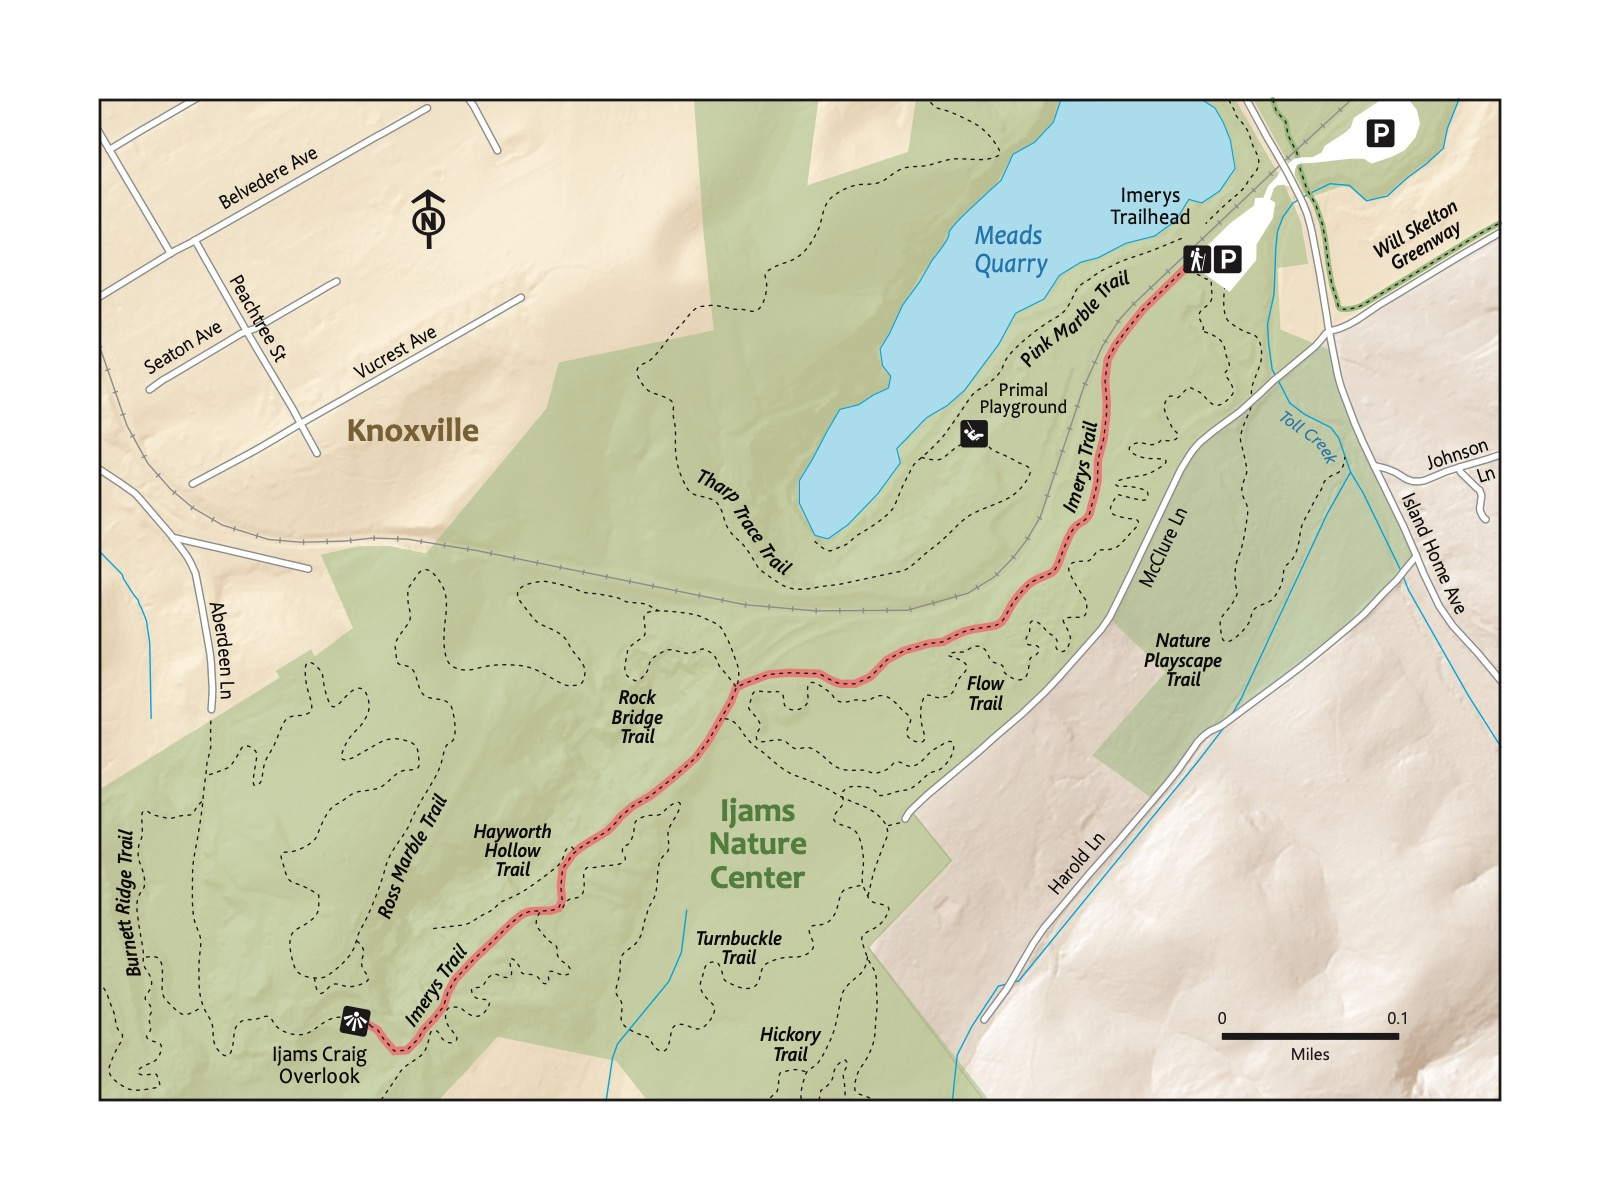
\includegraphics{maps/trail-08-map.jpeg}

\hypertarget{overview-7}{%
\subsubsection{Overview}\label{overview-7}}

This trail is a nice introduction to the half of Ijams that is centered
around Mead's Quarry -- what Ijams refers to as the Quarryside area The
hike begins at the quarry and winds up a smooth -- then rocky -- trail.
The overlook is for Ijams Crag, a popular outdoor rock climbing area. We
love having a snack at the shade of the pine trees at the overlook.
After winding back to the start, be sure to explore one of the two
excellent nature play areas nearby or take a side trail back to extend
the trip. It is hikable by older kids due to the rockiness and
steepness; younger kids may need a carry.

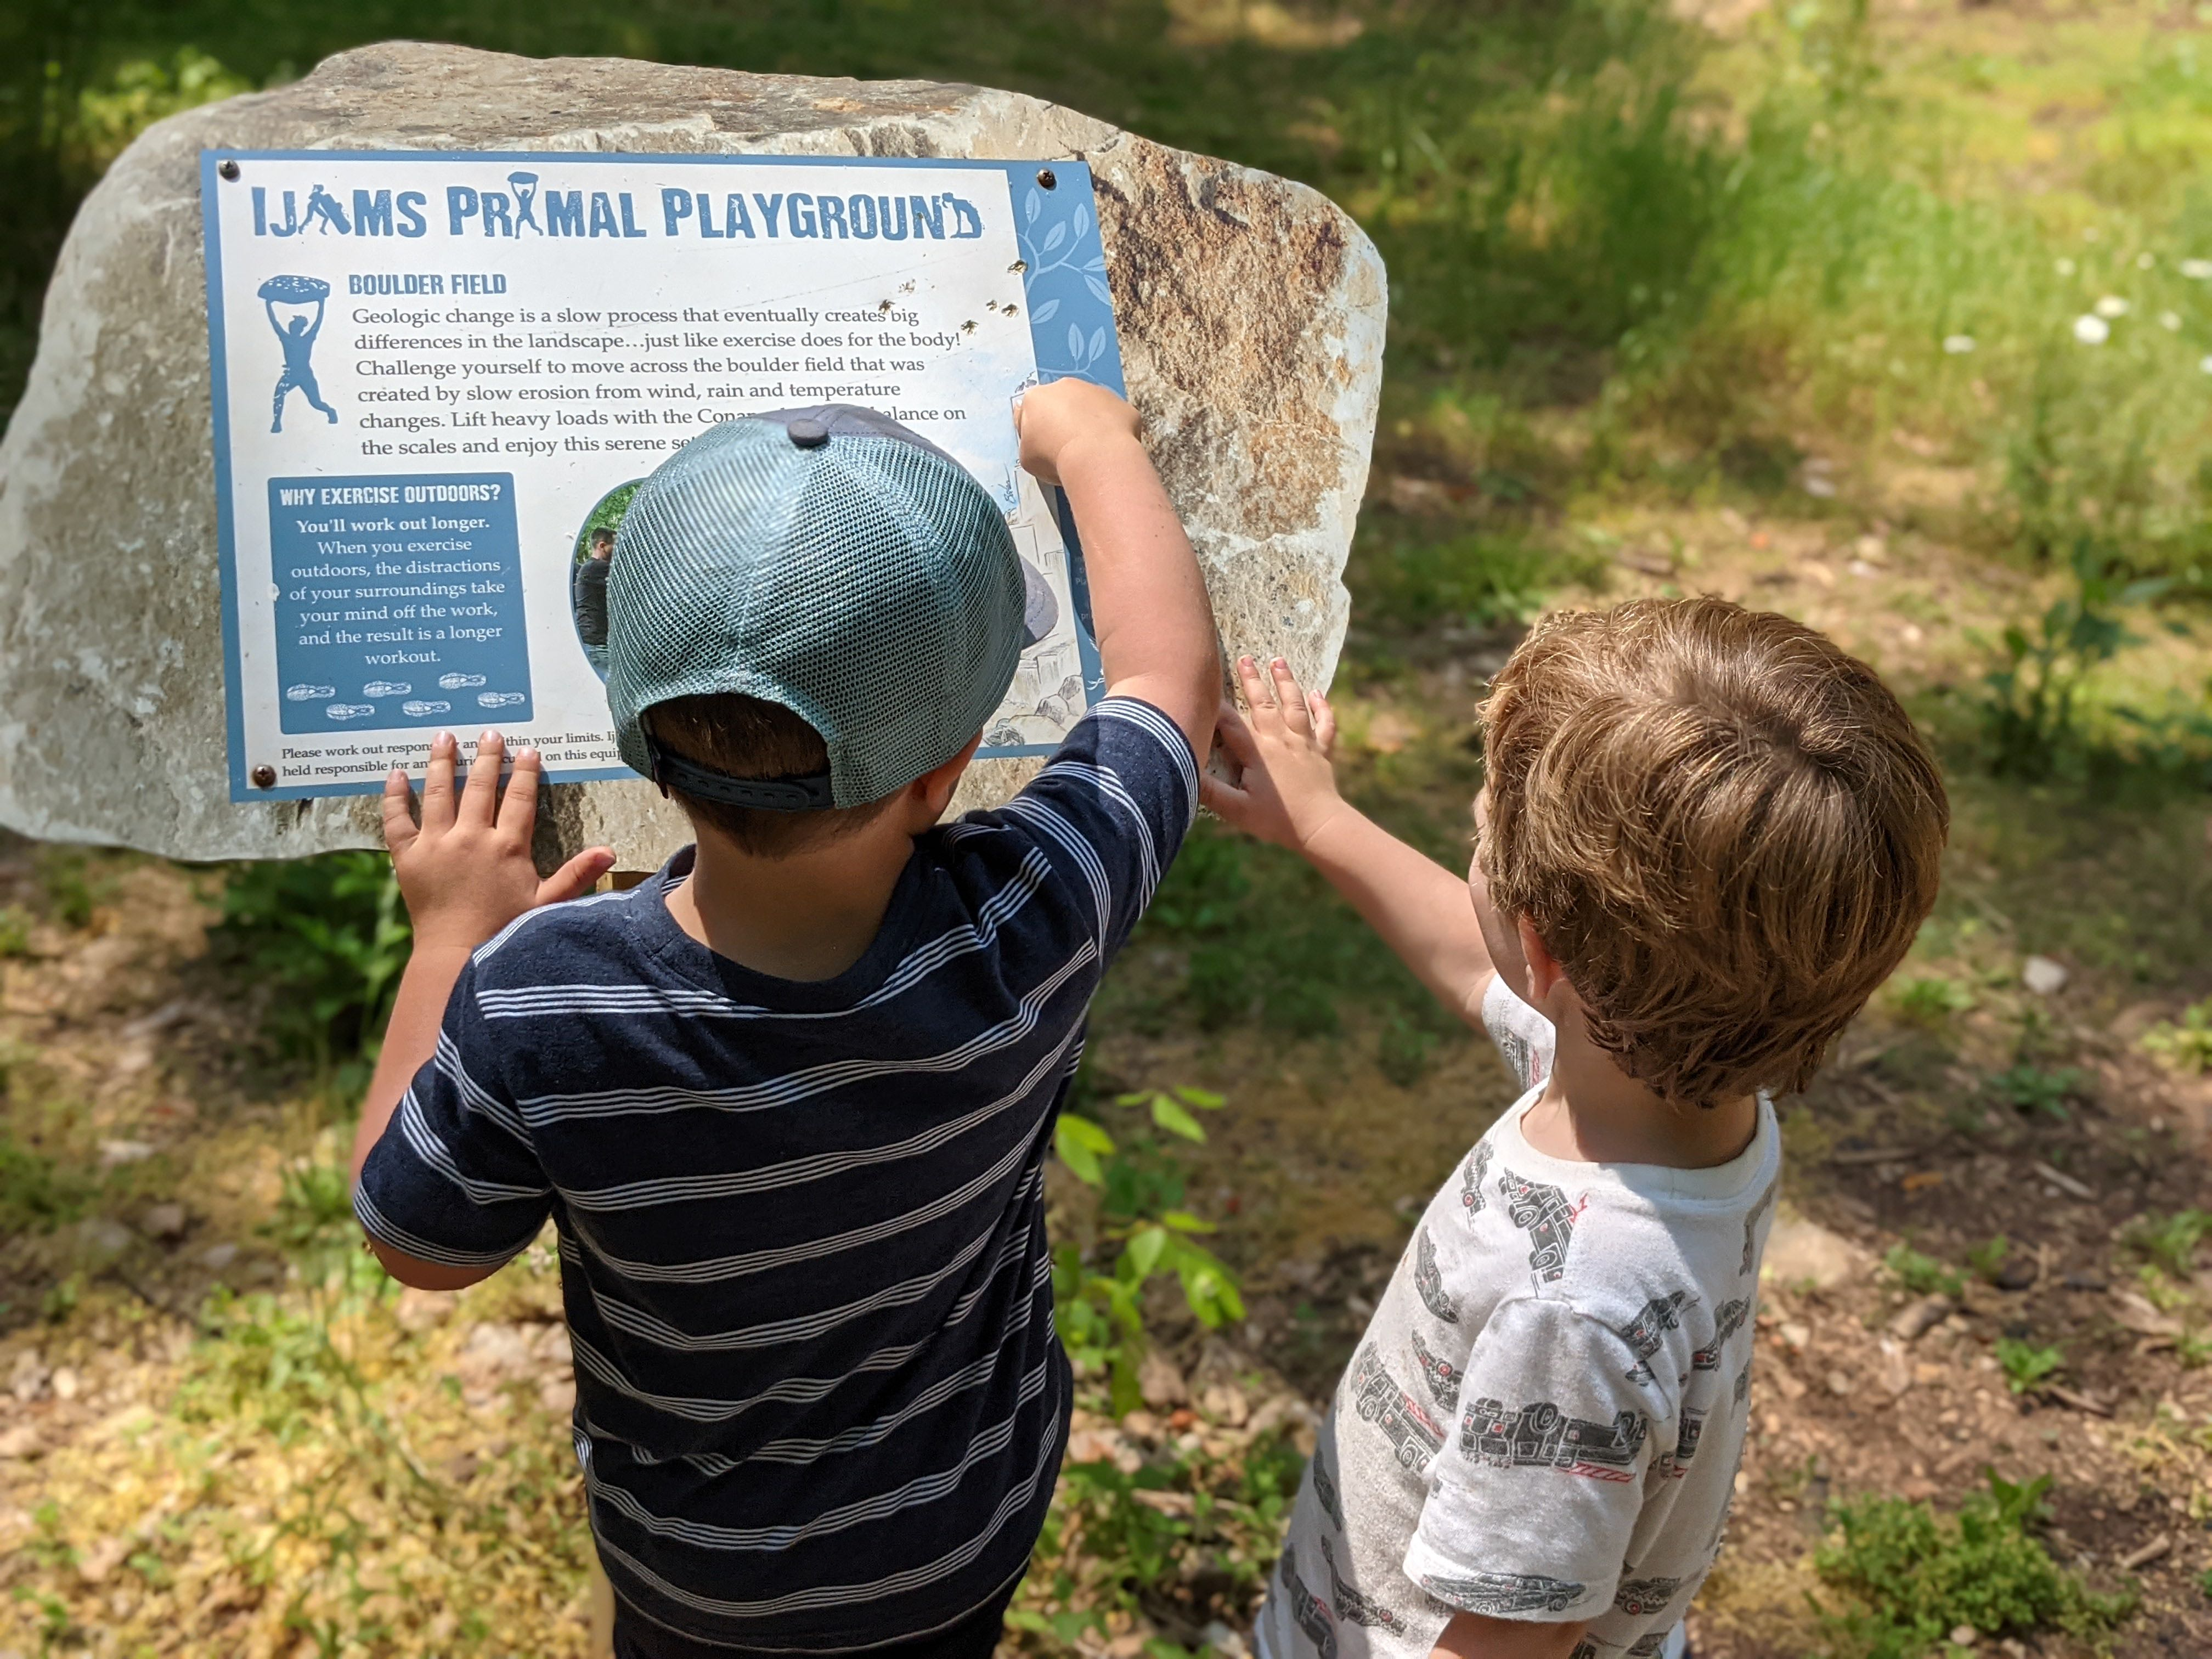
\includegraphics{img/trail-08-figure-01.jpg}

\hypertarget{directions-to-the-trailhead-7}{%
\subsubsection{Directions to the
Trailhead}\label{directions-to-the-trailhead-7}}

\begin{longtable}[]{@{}
  >{\raggedright\arraybackslash}p{(\columnwidth - 2\tabcolsep) * \real{0.5000}}
  >{\raggedright\arraybackslash}p{(\columnwidth - 2\tabcolsep) * \real{0.5000}}@{}}
\toprule\noalign{}
\begin{minipage}[b]{\linewidth}\raggedright
Trailhead Address
\end{minipage} & \begin{minipage}[b]{\linewidth}\raggedright
Meads Quarry, 3526 Island Home Ave, Knoxville, TN 37920
\end{minipage} \\
\midrule\noalign{}
\endhead
\bottomrule\noalign{}
\endlastfoot
Trailhead GPS Coordinates & 35.95174, -83.86587 \\
\end{longtable}

Park in the parking lot for Meads Quarry using the above address. The
trail begins alongside the disused railroad tracks; look for a sign for
Imery's.

\hypertarget{trail-description-7}{%
\subsubsection{Trail Description}\label{trail-description-7}}

\begin{longtable}[]{@{}
  >{\raggedright\arraybackslash}p{(\columnwidth - 2\tabcolsep) * \real{0.5000}}
  >{\raggedright\arraybackslash}p{(\columnwidth - 2\tabcolsep) * \real{0.5000}}@{}}
\toprule\noalign{}
\begin{minipage}[b]{\linewidth}\raggedright
Distance from Start
\end{minipage} & \begin{minipage}[b]{\linewidth}\raggedright
Description
\end{minipage} \\
\midrule\noalign{}
\endhead
\bottomrule\noalign{}
\endlastfoot
0.0 & Start on Imery's trail, heading away from the parking lot. \\
0.15 & Gradually, then more steeply. begin to ascend. \\
0.30 & Trail levels out at an intersection between Imery's Trail, Rock
Bridge Trail, and Gravel Road Trail. \\
0.5 & Rocky and steep. \\
0.75 & Reach the overlook to Ijams Quarry. Rest up, and then turn around
to head back --- or continue farther along on Imery's! \\
1.50 & Traihead. \\
\end{longtable}

\hypertarget{nearby-7}{%
\subsubsection{Nearby}\label{nearby-7}}

\begin{itemize}
\tightlist
\item
  Stopping by the Ijams Visitor Center. Check out the Ijams River and
  Tower loop for an introduction to this other area of the Ijams Nature
  Center.
\item
  Playing at the Ijams Nature Playscape. An amazing and surprising part
  of Ijams, worthy of a visit on its own. Tucked away a bit on the side
  of the parking area at Mead's Quarry. It's a favorite for kids, with a
  treehouse, tightrope, stumps for jumping, and---yes---a mud pit!
\item
  Playing at the Ijams Primal playground. Also nearby, smaller than the
  Nature Playground, but packed with features for climbing and jumping.
\end{itemize}

\hypertarget{trail-9-william-hastie}{%
\subsection{Trail 9: William Hastie}\label{trail-9-william-hastie}}

\hypertarget{key-characteristics-8}{%
\subsubsection{Key Characteristics}\label{key-characteristics-8}}

\begin{longtable}[]{@{}ll@{}}
\toprule\noalign{}
Trail Name & William Hastie \\
\midrule\noalign{}
\endhead
\bottomrule\noalign{}
\endlastfoot
Region & Knoxville and Surroundings \\
Trail \# & 9 \\
Time Estimate - Hiking Fast & 0.5 hours \\
Time Estimate - Hiking Slowly & 1 hour \\
Trail Distance (Miles) & 1.3 \\
Elevation Change & Flat \\
Pets & Allowed on leash \\
Parking Pass/Entrance Fee & Not Required \\
Restroom(s) & No \\
Terrain & Gravel path \\
\end{longtable}

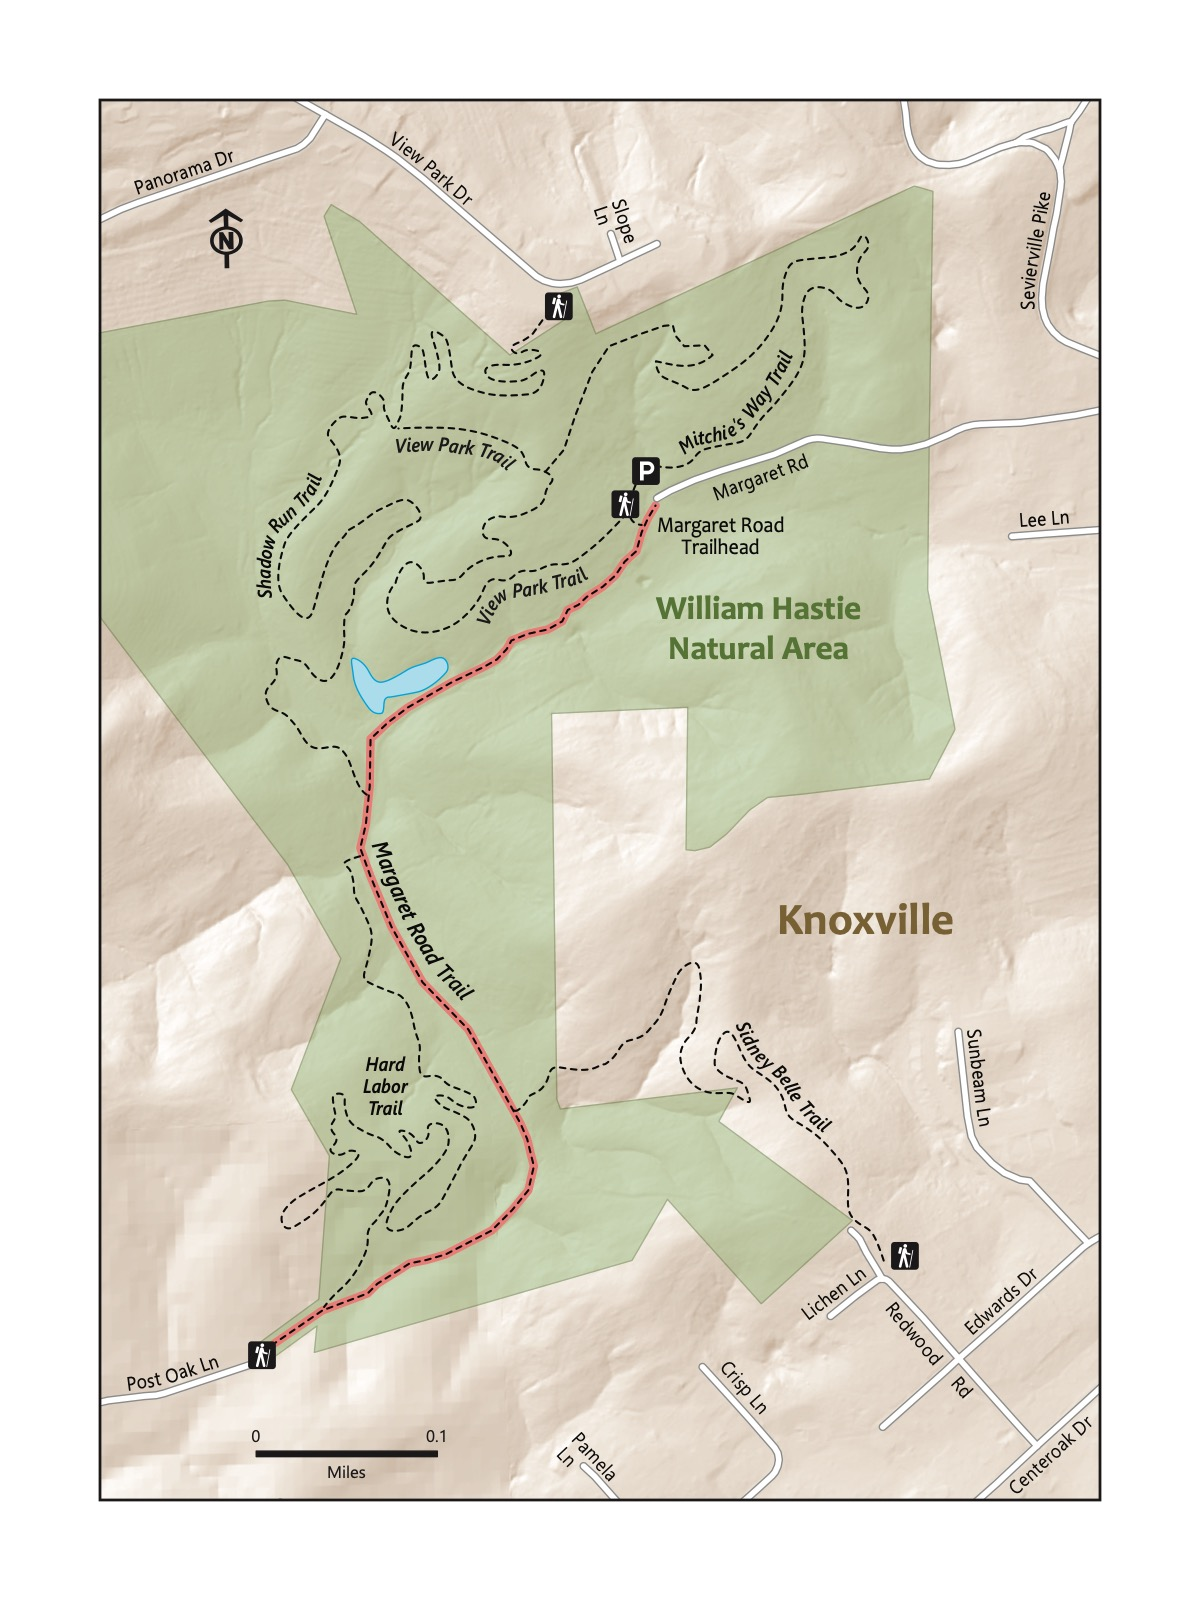
\includegraphics{maps/trail-09-map.jpeg}

\hypertarget{overview-8}{%
\subsubsection{Overview}\label{overview-8}}

A short walk on a gravel path through deep woods. The start features a
beginner's mountain bike loop on a smooth path; consider bringing kids'
bikes. Though short, this hike takes you by many spur trails; consider
this a gentle introduction to a trail system close to but more rustic
than Ijams. Good for all toddling and walking kids and their families.

\includegraphics{img/trail-09-figure-01.jpg}

\hypertarget{directions-to-the-trailhead-8}{%
\subsubsection{Directions to the
Trailhead}\label{directions-to-the-trailhead-8}}

\begin{longtable}[]{@{}
  >{\raggedright\arraybackslash}p{(\columnwidth - 2\tabcolsep) * \real{0.5000}}
  >{\raggedright\arraybackslash}p{(\columnwidth - 2\tabcolsep) * \real{0.5000}}@{}}
\toprule\noalign{}
\begin{minipage}[b]{\linewidth}\raggedright
Trailhead Address
\end{minipage} & \begin{minipage}[b]{\linewidth}\raggedright
William Hastie Natural Area, 1302 Margaret Rd, Knoxville, TN 37920
\end{minipage} \\
\midrule\noalign{}
\endhead
\bottomrule\noalign{}
\endlastfoot
Trailhead GPS Coordinates & 35.93464, -83.87455 \\
\end{longtable}

The above address will direct you to a large, rarely-busy parking area
and a nice trailhead with a picnic area. Several trails start from this
trailhead. Look for a sign for the Margaret Road Trail.

\hypertarget{trail-description-8}{%
\subsubsection{Trail Description}\label{trail-description-8}}

\begin{longtable}[]{@{}
  >{\raggedright\arraybackslash}p{(\columnwidth - 2\tabcolsep) * \real{0.2917}}
  >{\raggedright\arraybackslash}p{(\columnwidth - 2\tabcolsep) * \real{0.7083}}@{}}
\toprule\noalign{}
\begin{minipage}[b]{\linewidth}\raggedright
Distance from Start
\end{minipage} & \begin{minipage}[b]{\linewidth}\raggedright
Description
\end{minipage} \\
\midrule\noalign{}
\endhead
\bottomrule\noalign{}
\endlastfoot
0.0 & Start on the Margaret Road Trail. \\
0.2 & Small pond on the right. Look for turtles! \\
0.25 & Shadow Run Trail on the right. \\
0.65 & Reach the Post Oak Ln. Trailhead and turn around. \\
1.30 & Traihead. \\
\end{longtable}

\hypertarget{nearby-8}{%
\subsubsection{Nearby}\label{nearby-8}}

\begin{itemize}
\tightlist
\item
  Biking on the kids' loop. The ``green'' mountain biking trail,
  Springarn, is a great spot for kids to begin to learn to ride on
  trails. It's only 0.6 miles and is a nice complement to this hike.
\item
  Exploring some of the many other trails. William Hastie Natural Area
  features a ton of other trails. Consider taking Mitchie's Way from
  near the parking area --- and then looping back to Margaret Road and
  the start on the trail of your choice.
\end{itemize}

\hypertarget{trail-10-sharps-ridge}{%
\subsection{Trail 10: Sharp's Ridge}\label{trail-10-sharps-ridge}}

\hypertarget{key-characteristics-9}{%
\subsubsection{Key Characteristics}\label{key-characteristics-9}}

\begin{longtable}[]{@{}ll@{}}
\toprule\noalign{}
Trail Name & Sharp's Ridge Overlook \\
\midrule\noalign{}
\endhead
\bottomrule\noalign{}
\endlastfoot
Region & Knoxville and Surroundings \\
Trail \# & 10 \\
Time Estimate - Hiking Fast & 1.5 hours \\
Time Estimate - Hiking Slowly & 2.5 hours \\
Trail Distance (Miles) & 2.3 \\
Elevation Change & Moderate \\
Pets & Allowed on leash \\
Parking Pass/Entrance Fee & Not Required \\
Restroom(s) & No \\
Terrain & Dirt path; road \\
\end{longtable}

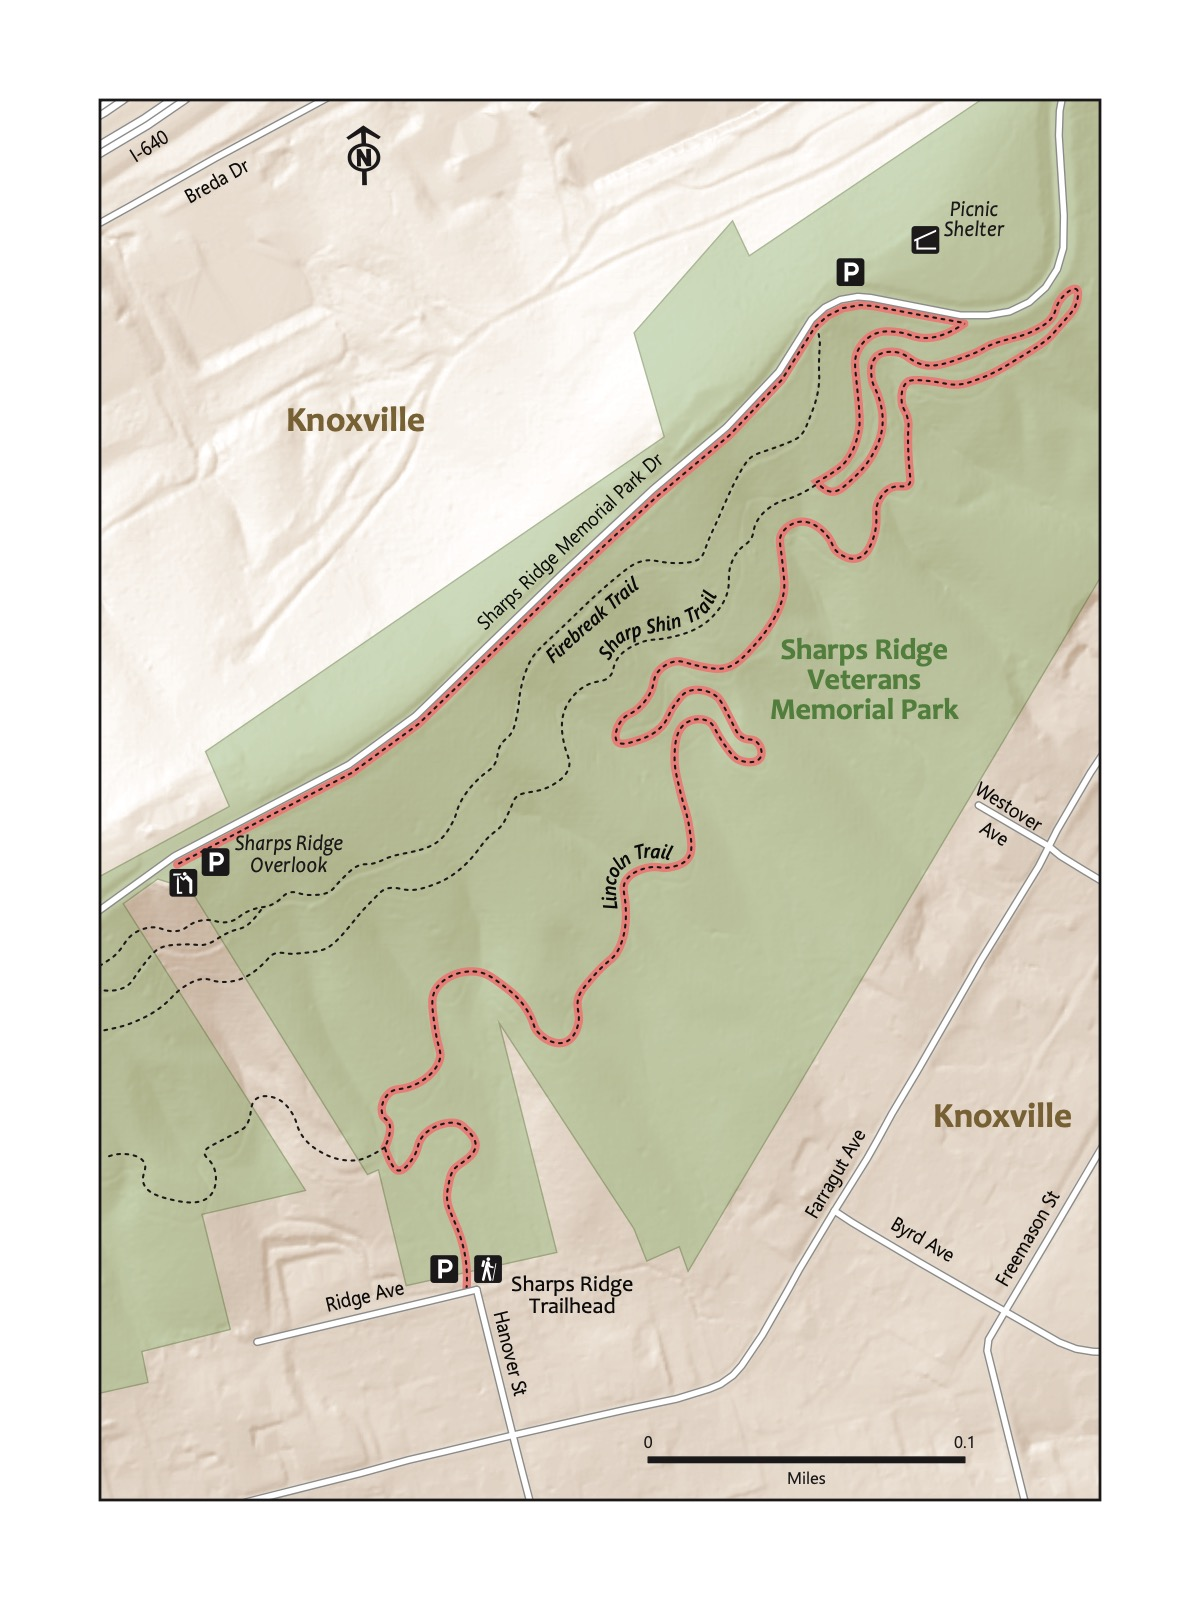
\includegraphics{maps/trail-10-map.jpeg}

\hypertarget{overview-9}{%
\subsubsection{Overview}\label{overview-9}}

A hike that starts very close to the city center of Knoxville -- just
north. Wind up from the trailhead on a smooth path through the pretty
forest. When we think of this trail, we think of little ones toddling or
running ahead around the bends in the trail, just far enough to be out
of sight for a little bit until we catch up! Connect to the road and --
optionally -- walk up to an overlook from which the Smokies are visible.
A short but sweet family hike that's close to many amenities. Best for
older kids or younger kids who are carried.

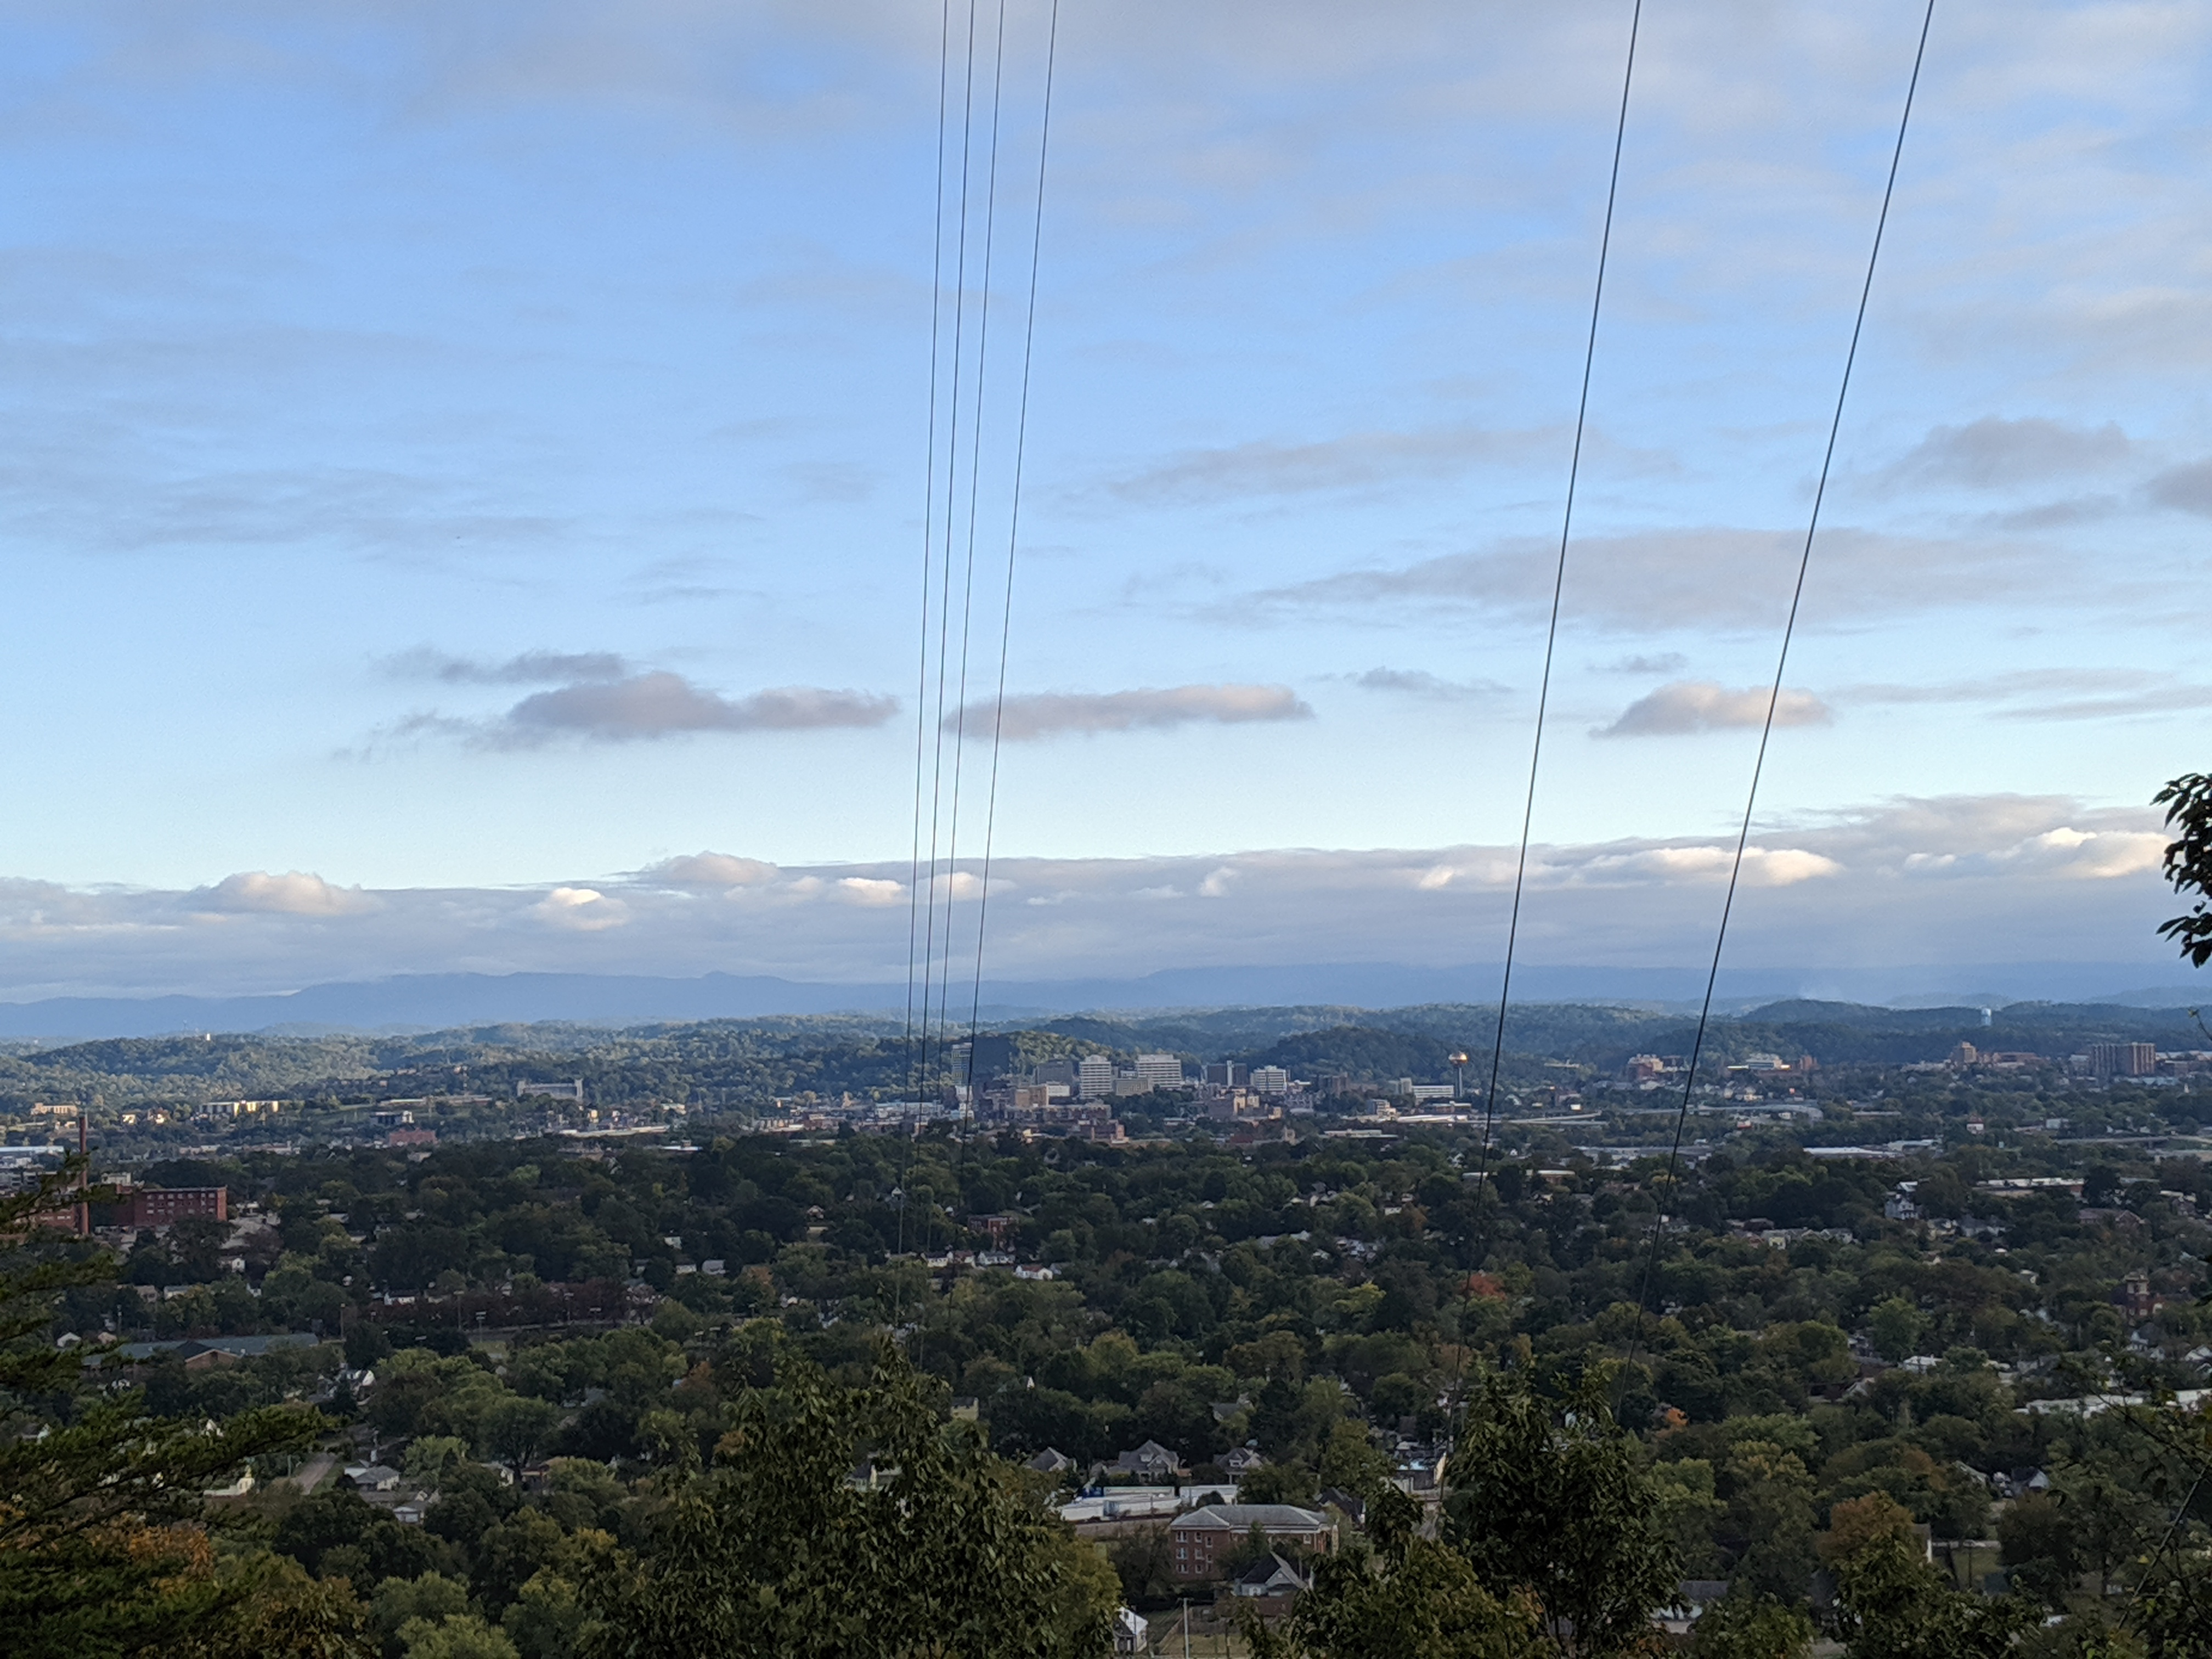
\includegraphics{img/trail-10-figure-01.jpg}

\hypertarget{directions-to-the-trailhead-9}{%
\subsubsection{Directions to the
Trailhead}\label{directions-to-the-trailhead-9}}

\begin{longtable}[]{@{}
  >{\raggedright\arraybackslash}p{(\columnwidth - 2\tabcolsep) * \real{0.5000}}
  >{\raggedright\arraybackslash}p{(\columnwidth - 2\tabcolsep) * \real{0.5000}}@{}}
\toprule\noalign{}
\begin{minipage}[b]{\linewidth}\raggedright
Trailhead Address
\end{minipage} & \begin{minipage}[b]{\linewidth}\raggedright
Sharps Ridge Trailhead, 599-501 Ridge Ave, Knoxville, TN 37917
\end{minipage} \\
\midrule\noalign{}
\endhead
\bottomrule\noalign{}
\endlastfoot
Trailhead GPS Coordinates & 36.00344, -83.93787 \\
\end{longtable}

The trailhead can be just a little tricky to find---partially because
Google Maps has several trailheads with the same name! We once met
friends at different Sharps Ridge Trailheads! Consider putting in the
address (above) to find the trailhead, which is at the end of Hanover
St.~Park in one of the parking spots or the gravel area on the side of
Ridge Ave.

\hypertarget{trail-description-9}{%
\subsubsection{Trail Description}\label{trail-description-9}}

\begin{longtable}[]{@{}
  >{\raggedright\arraybackslash}p{(\columnwidth - 2\tabcolsep) * \real{0.5000}}
  >{\raggedright\arraybackslash}p{(\columnwidth - 2\tabcolsep) * \real{0.5000}}@{}}
\toprule\noalign{}
\begin{minipage}[b]{\linewidth}\raggedright
Distance from Start
\end{minipage} & \begin{minipage}[b]{\linewidth}\raggedright
Description
\end{minipage} \\
\midrule\noalign{}
\endhead
\bottomrule\noalign{}
\endlastfoot
0.0 & Start by walking through the Arbor, past the handy trail map of
the Sharps Ridge area. You're technically on the very short Hanover
Access trail. \\
0.1 & Turn right onto Lincoln Trail. Wind up through the deep woods and
easy curves in the trail. \\
0.8 & Turn right onto Sharp Shin. \\
0.9 & Meet Sharps Ridge Memorial Park Drive, a road. Turn left to walk
along the side of the road toward the overlook --- or, alternatively,
head back to the start! \\
1.15 & Overlook. See if you can spy the Sunsphere, Neyland Stadium, and
the Smokies in the distance. Turn around to head back the way you
came. \\
1.4 & Turn right, back onto Sharp Shin. \\
1.5 & Turn left onto Lincoln Trail. \\
2.2 & Turn left onto the Hanover Access Trail. \\
2.3 & Traihead. \\
\end{longtable}

\hypertarget{nearby-9}{%
\subsubsection{Nearby}\label{nearby-9}}

\begin{itemize}
\tightlist
\item
  Stopping at nearby restaurants and shops. Favorite nearby spots
  include the fantastic Wild Love Bakehouse (1625 N Central St,
  Knoxville, TN 37917), the quick, inexpensive, tasty Taqueria La
  Herradura (2625 N Broadway, Knoxville, TN 37917), and Hard Knox Pizza
  Central (2300 N Central St, Knoxville, TN 37917).
\item
  Hiking further or on other trails. Sharp's Ridge includes tons of
  other trails. A favorite starts at a different---but nearby---parking
  area, immediately behind the Cherry Creek Apartments (navigate to 3404
  Dill St, Knoxville, TN 37917). We like the Lincoln Trail, which is an
  accessible mountain bike trail.
\end{itemize}

\hypertarget{trail-11-norris-dam}{%
\subsection{Trail 11: Norris Dam}\label{trail-11-norris-dam}}

\hypertarget{key-characteristics-10}{%
\subsubsection{Key Characteristics}\label{key-characteristics-10}}

\begin{longtable}[]{@{}ll@{}}
\toprule\noalign{}
Trail Name & Songbird Loop \\
\midrule\noalign{}
\endhead
\bottomrule\noalign{}
\endlastfoot
Region & Knoxville and Surroundings \\
Trail \# & 11 \\
Time Estimate - Hiking Fast & 1.5 hours \\
Time Estimate - Hiking Slowly & 2.5 hours \\
Trail Distance (Miles) & 2.3 \\
Elevation Change & Gentle \\
Pets & Allowed on leash \\
Parking Pass/Entrance Fee & Not Required \\
Restroom(s) & No \\
Terrain & Gravel path \\
\end{longtable}

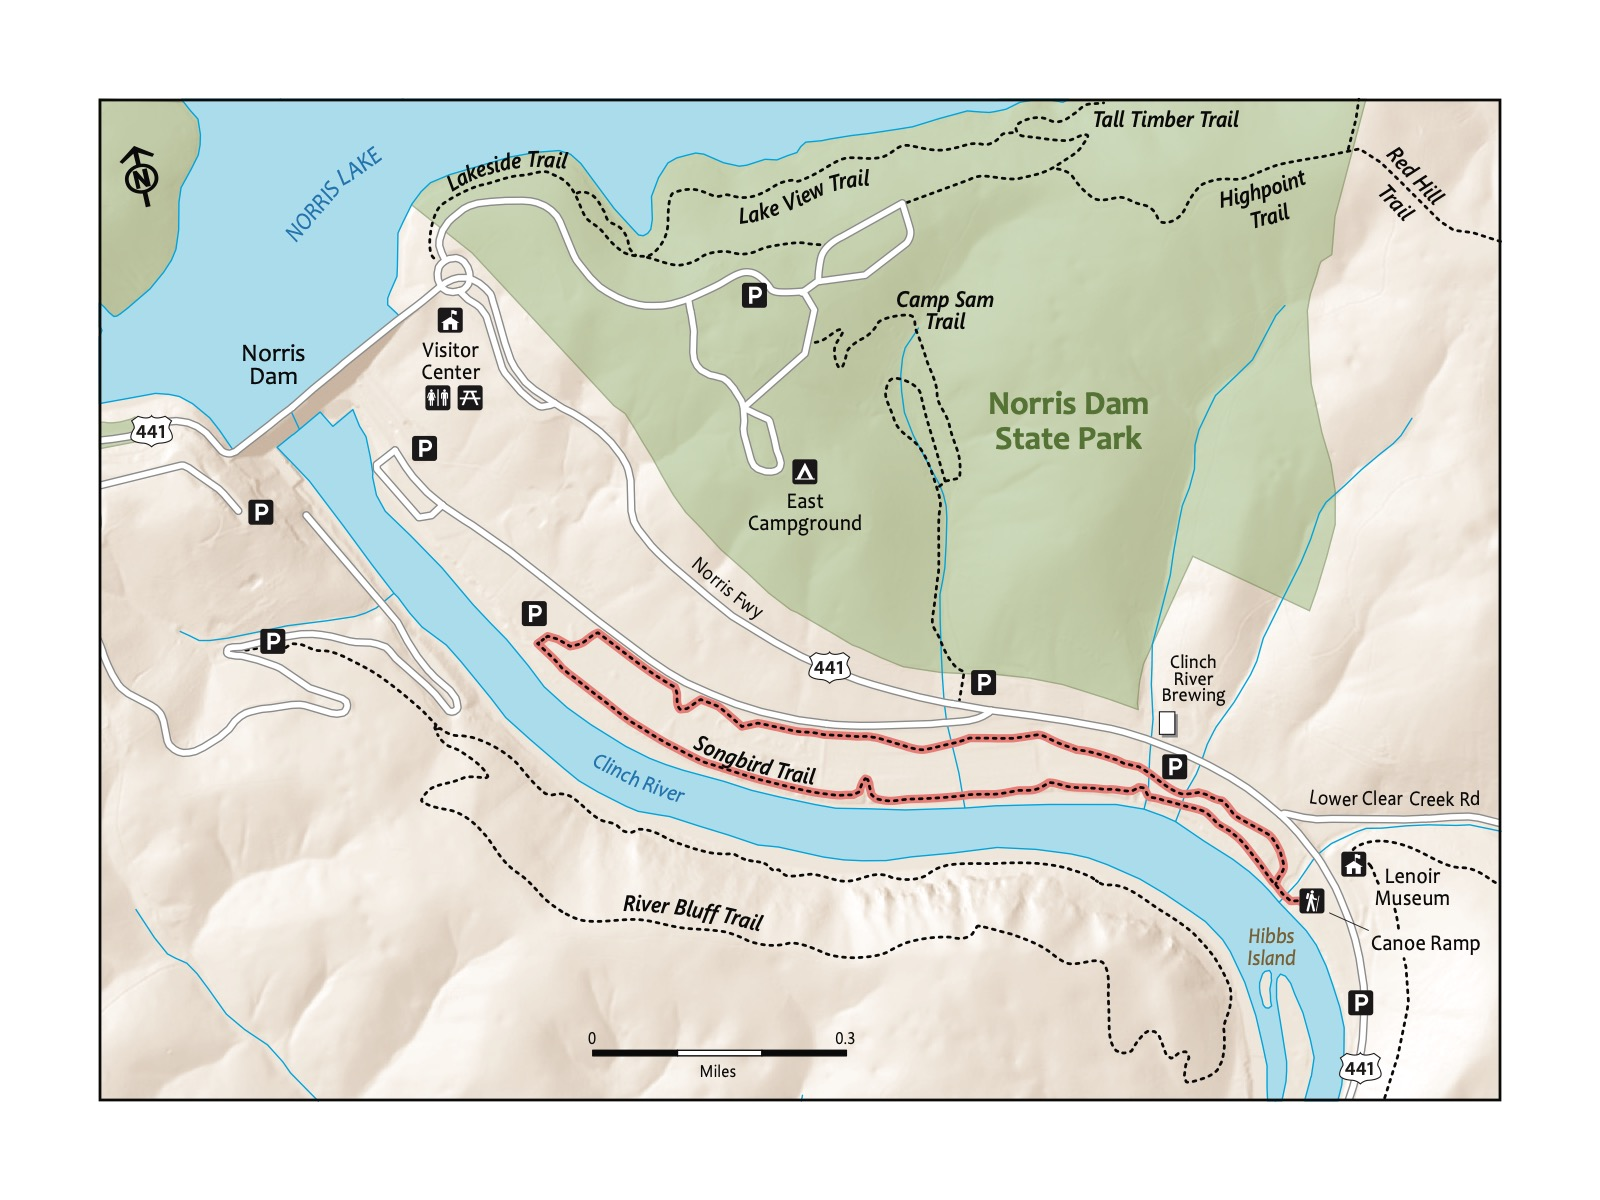
\includegraphics{maps/trail-11-map.jpeg}

\hypertarget{overview-10}{%
\subsubsection{Overview}\label{overview-10}}

Part of Norris Dam State Park, around thirty minutes north of Knoxville
on the pretty Norris Lake. This hike is one of the flattest we feature.
Further, it's on a graded gravel path. Like the Knox-Blount Greenway
along the Tennessee River, you may be surprised by the variety and
quantity of wildlife you see along this scenic river, the Clinch. A
relaxing trail for a family outing that might end with a drive over
Norris Dam or a stop for a bite and a drink at the nearby Clinch River
Brewery. This hike would be a fun challenge for the toddler ready to
hike a bit farther.

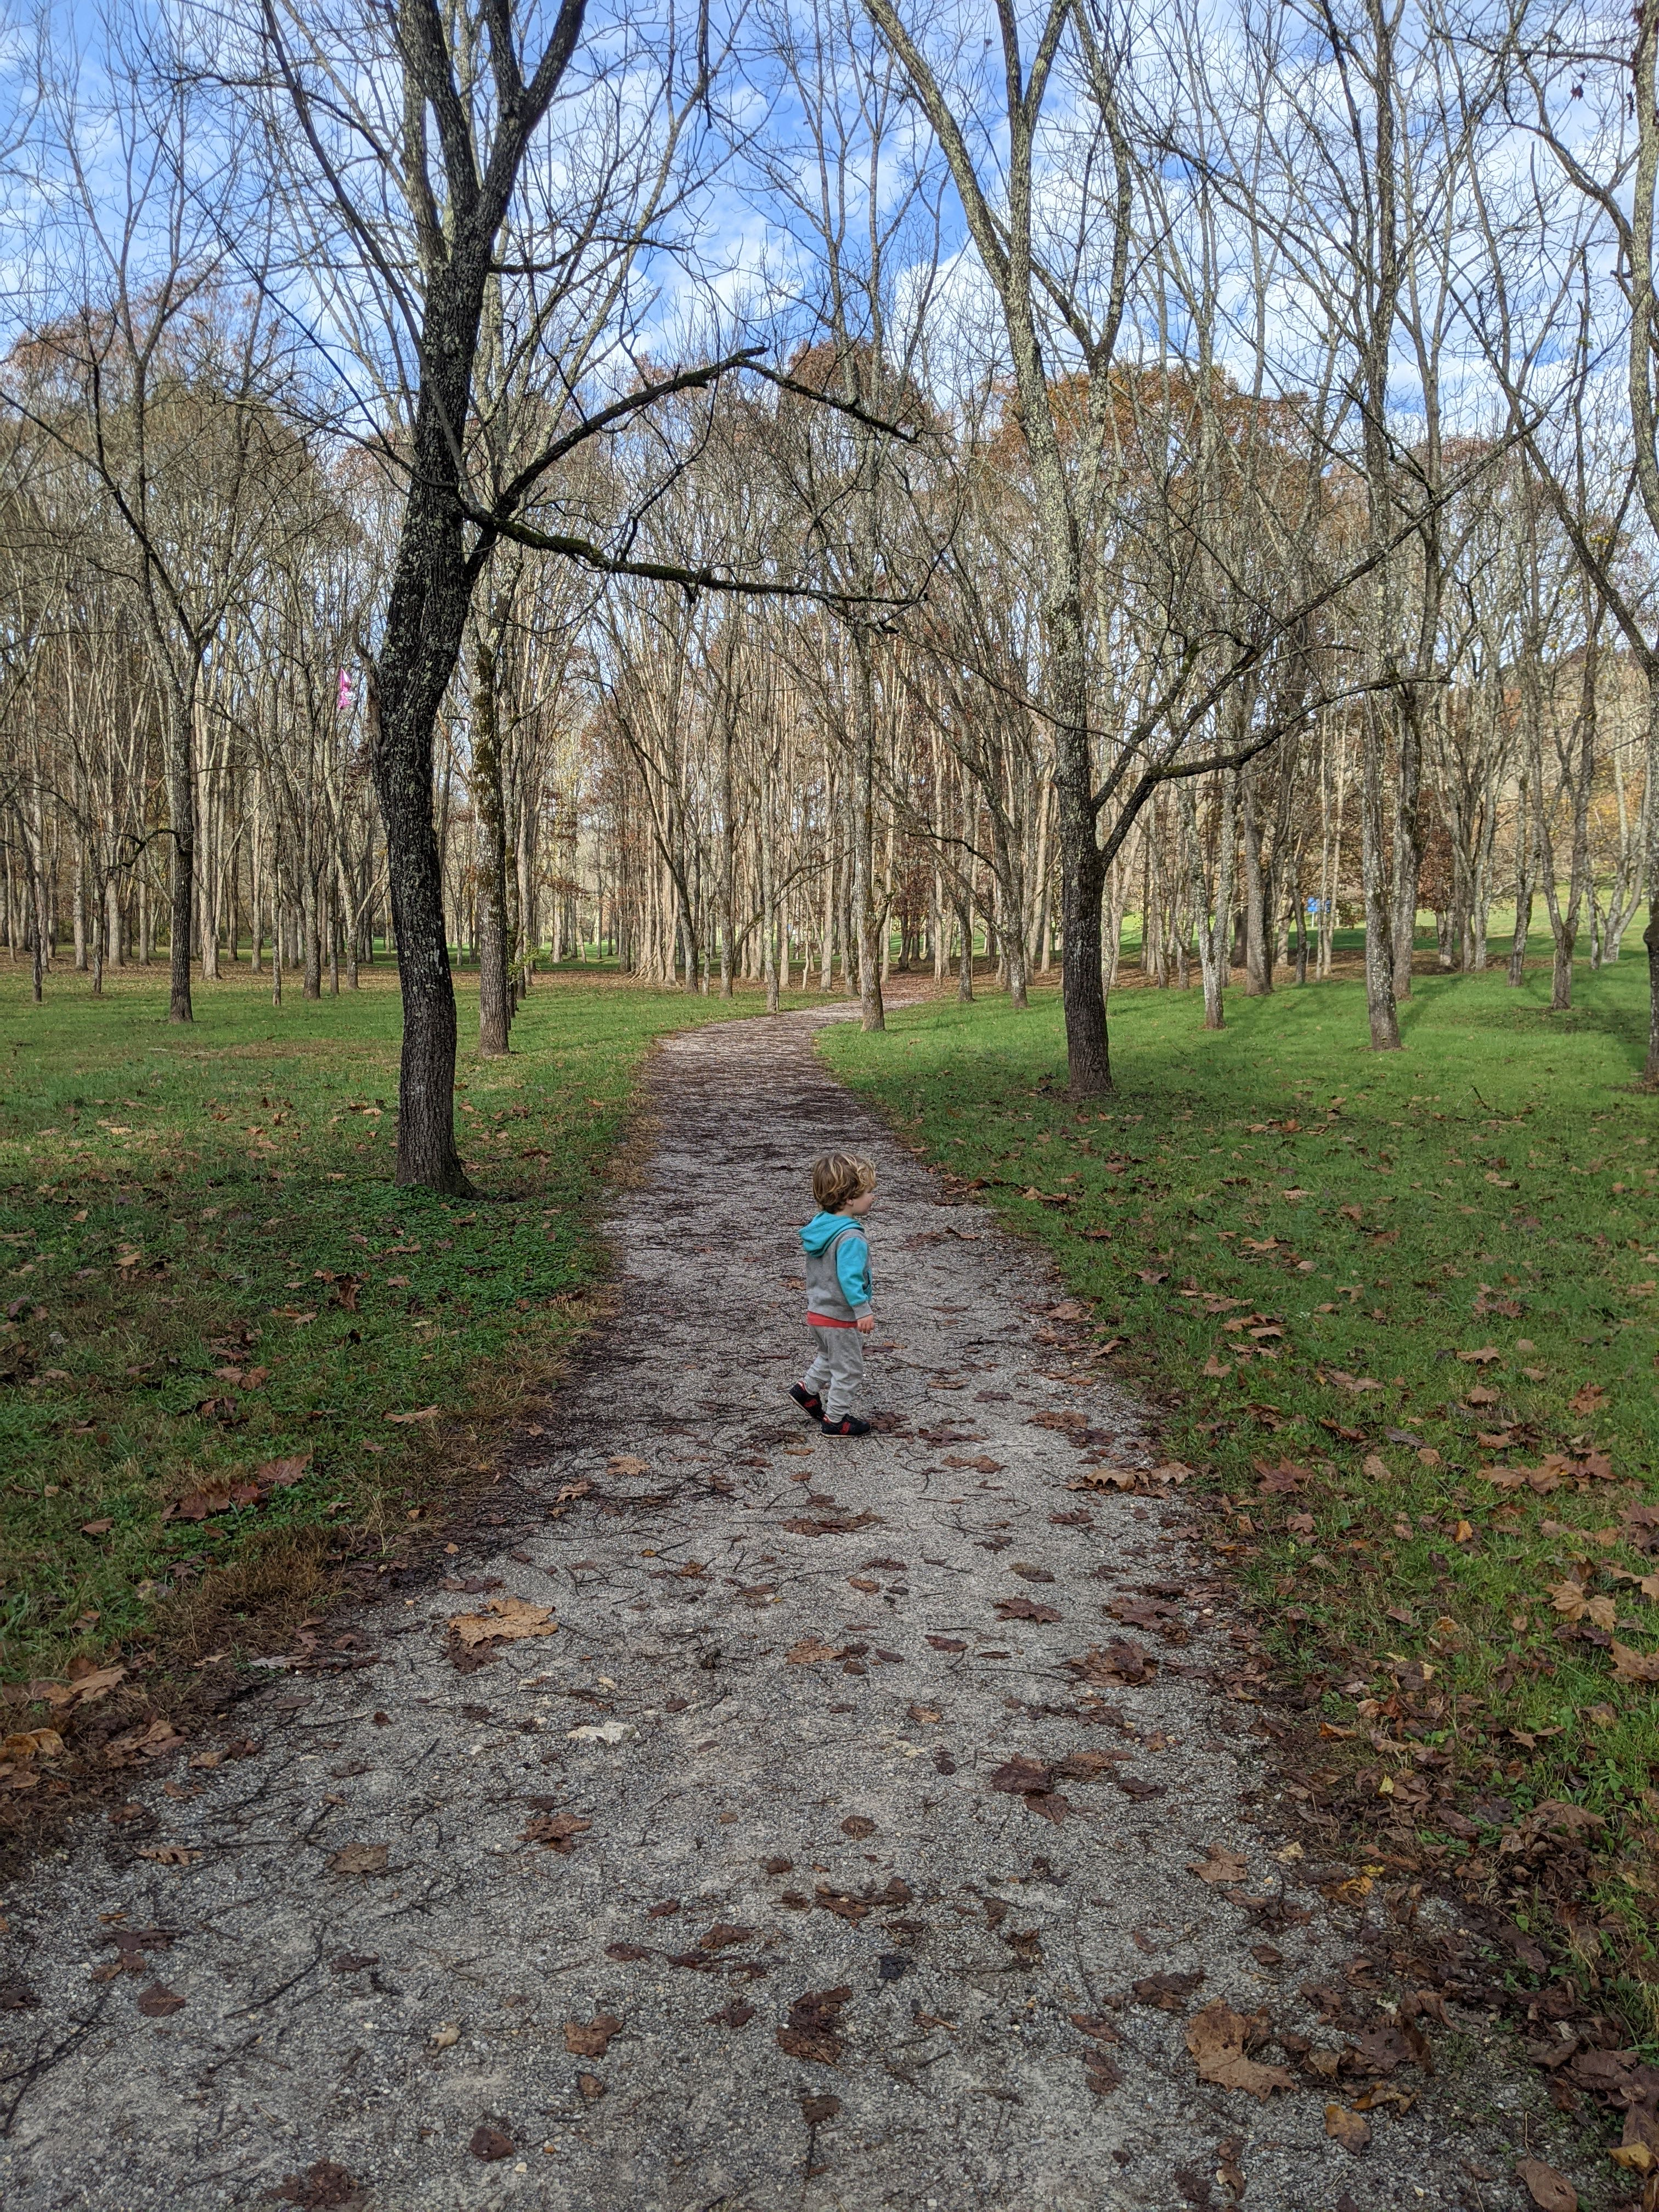
\includegraphics{img/trail-11-figure-01.jpg}

\hypertarget{directions-to-the-trailhead-10}{%
\subsubsection{Directions to the
Trailhead}\label{directions-to-the-trailhead-10}}

\begin{longtable}[]{@{}
  >{\raggedright\arraybackslash}p{(\columnwidth - 2\tabcolsep) * \real{0.5000}}
  >{\raggedright\arraybackslash}p{(\columnwidth - 2\tabcolsep) * \real{0.5000}}@{}}
\toprule\noalign{}
\begin{minipage}[b]{\linewidth}\raggedright
railhead Address
\end{minipage} & \begin{minipage}[b]{\linewidth}\raggedright
Canoe Ramp by the Songbird Loop, 6W6G+R7 Rocky Top, Tennessee
\end{minipage} \\
\midrule\noalign{}
\endhead
\bottomrule\noalign{}
\endlastfoot
Trailhead GPS Coordinates & 36.21210, -84.07397 \\
\end{longtable}

There are several possible trailheads, all easy to access. We chose to
start this hike from a put in spot for kayaks and canoes. In Google
Maps, you can search the above address. Please note it uses a ``Plus
code'' instead of a street address, as the canoe ramp does not have an
address. This is immediately off Norris Fwy. (Highway 441) ---
curiously, the same highway that bisects the Smokies. Park in the large
parking lot and head toward the river.

\hypertarget{trail-description-10}{%
\subsubsection{Trail Description}\label{trail-description-10}}

\begin{longtable}[]{@{}
  >{\raggedright\arraybackslash}p{(\columnwidth - 2\tabcolsep) * \real{0.5000}}
  >{\raggedright\arraybackslash}p{(\columnwidth - 2\tabcolsep) * \real{0.5000}}@{}}
\toprule\noalign{}
\begin{minipage}[b]{\linewidth}\raggedright
Distance from Start
\end{minipage} & \begin{minipage}[b]{\linewidth}\raggedright
Description
\end{minipage} \\
\midrule\noalign{}
\endhead
\bottomrule\noalign{}
\endlastfoot
0.0 & Start by crossing a short bridge over Clear Creek. \\
0.05 & Turn right to start the loop in a counterclockwise fashion (of
course, you can hike the other way, too!). \\
0.3 & Short bridge. \\
1.0 & Turn left, toward the river, remaining on the same trail. \\
1.05 & Follow the trail back along the river. \\
2.3 & Trailhead. \\
\end{longtable}

\hypertarget{nearby-10}{%
\subsubsection{Nearby}\label{nearby-10}}

\begin{itemize}
\tightlist
\item
  Stopping by the Clinch River Brewery. Clinch River Brewing (2045
  Norris Fwy, Norris, TN 37828) is not within the boundaries of the
  Norris Dam State Park---but it's very close to the trailhead and is a
  fun place to stop for lunch or dinner before or after a hike.
\item
  Checking out Norris Dam. Stop at the TVA Norris Dam Visitor Center on
  the same side of the Clinch River as this hike --- or drive across and
  back over the dam for an impressive---and a bit of an
  otherworldly---view and experience.
\end{itemize}

\hypertarget{trail-12-house-mountain}{%
\subsection{Trail 12: House Mountain}\label{trail-12-house-mountain}}

\hypertarget{key-characteristics-11}{%
\subsubsection{Key Characteristics}\label{key-characteristics-11}}

\begin{longtable}[]{@{}ll@{}}
\toprule\noalign{}
Trail Name & House Mountain Overlook \\
\midrule\noalign{}
\endhead
\bottomrule\noalign{}
\endlastfoot
Region & Knoxville and Surroundings \\
Trail \# & 12 \\
Time Estimate - Hiking Fast & 2.5 hours \\
Time Estimate - Hiking Slowly & 4.5 hours \\
Trail Distance (Miles) & 2.5 \\
Elevation Change & Steep \\
Pets & Allowed on leash \\
Parking Pass/Entrance Fee & Not Required \\
Restroom(s) & No \\
Terrain & Dirt path; rocky path \\
\end{longtable}

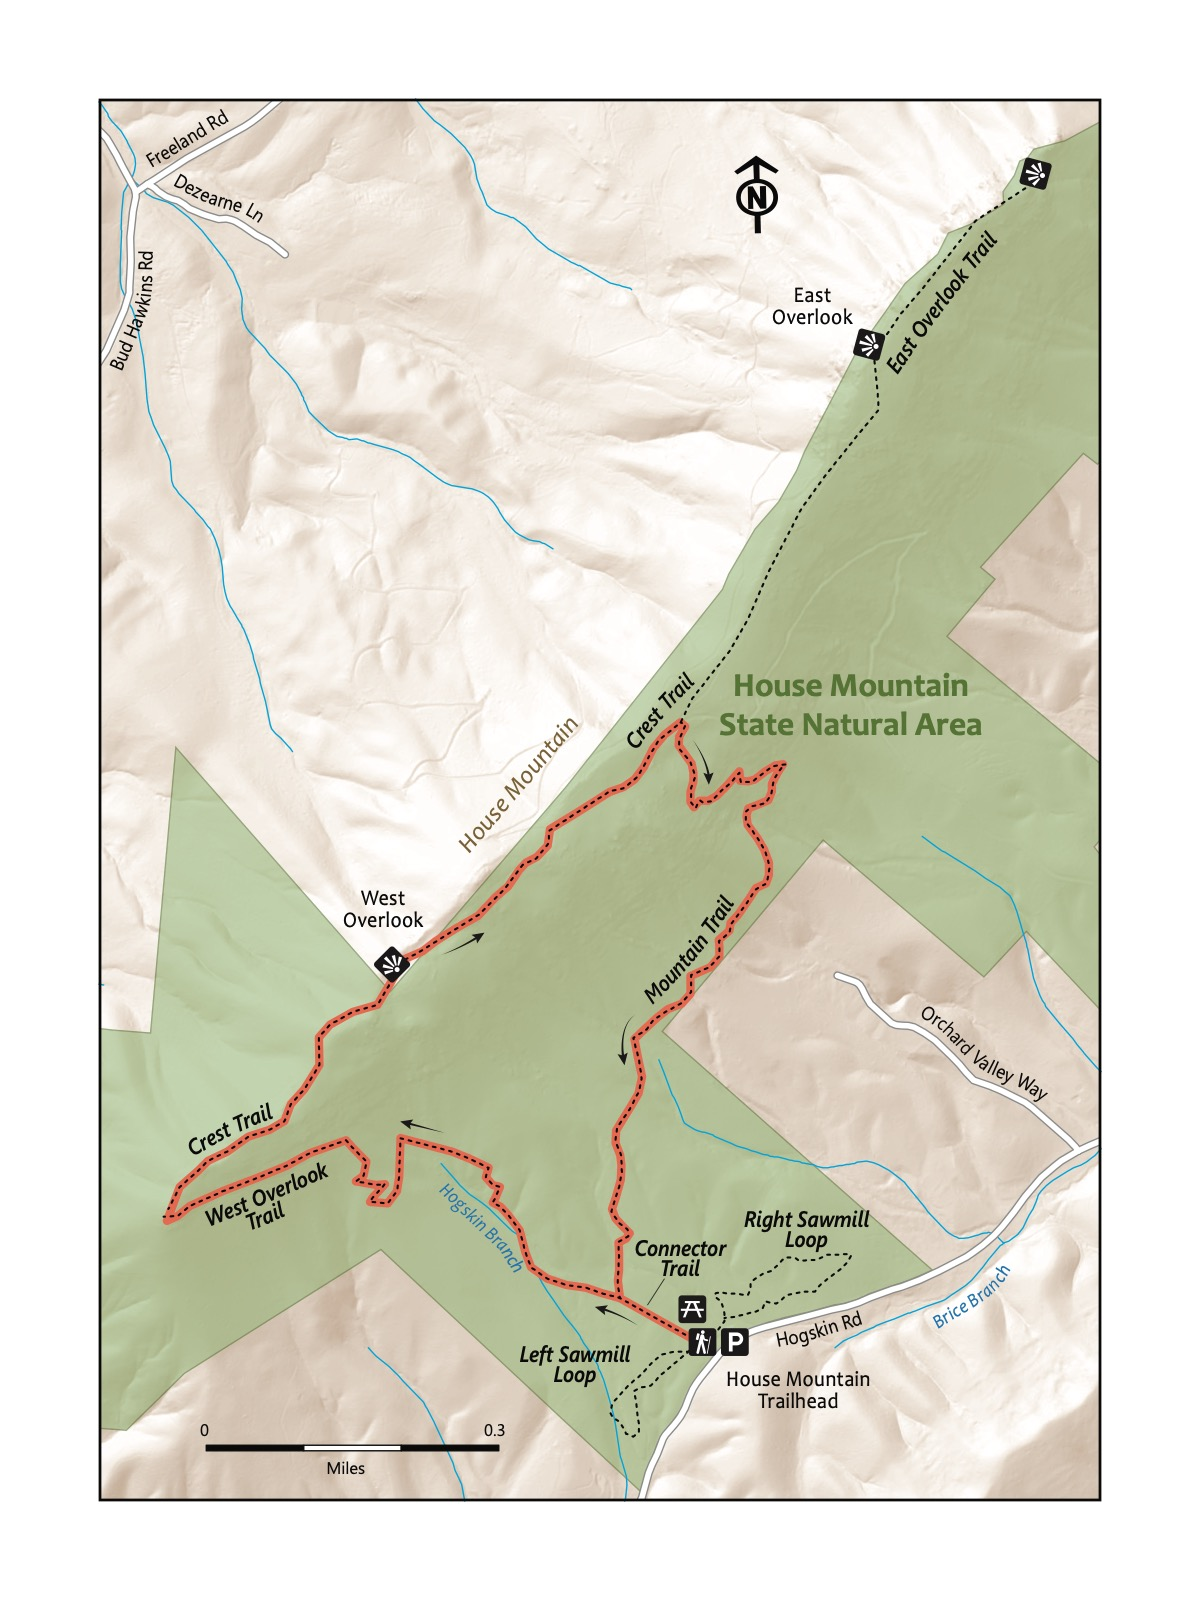
\includegraphics{maps/trail-12-map.jpeg}

\hypertarget{overview-11}{%
\subsubsection{Overview}\label{overview-11}}

The highest point in Knox County (but far from the highest in the book),
this trail feels like it belongs in another section of the book. The
elevation gain is substantial, and the trail is rockier and rougher than
the others close to Knoxville. This one always challenges us! But, the
flip side is that House Mountain offers a challenging hike to a
rewarding overlook far nearer to Knoxville than those in the Cumberland
Plateau or the Great Smoky Mountains National Park. The trail climbs up
House Mountain from the west, reaching the West Overlook before heading
down to complete the clockwise loop (you're free to hike it in the
opposite direction). Good for older kids or families able to carry a
little one a farther distance.

{[}Credit to Hanhui Bao{]}{[}/img/trail-12-figure-01.jpg{]}

\hypertarget{directions-to-the-trailhead-11}{%
\subsubsection{Directions to the
Trailhead}\label{directions-to-the-trailhead-11}}

\begin{longtable}[]{@{}
  >{\raggedright\arraybackslash}p{(\columnwidth - 2\tabcolsep) * \real{0.5000}}
  >{\raggedright\arraybackslash}p{(\columnwidth - 2\tabcolsep) * \real{0.5000}}@{}}
\toprule\noalign{}
\begin{minipage}[b]{\linewidth}\raggedright
Trailhead Address
\end{minipage} & \begin{minipage}[b]{\linewidth}\raggedright
House Mountain Parking and Trailhead, 463P+WV Corryton, Tennessee
\end{minipage} \\
\midrule\noalign{}
\endhead
\bottomrule\noalign{}
\endlastfoot
Trailhead GPS Coordinates & 36.10483, -83.76276 \\
\end{longtable}

The trailhead is straightforward to locate and access. Park at the large
parking area and look for the large covered picnic area. Look for the
Connector Trail near the picnic area to begin the hike.

\hypertarget{trail-description-11}{%
\subsubsection{Trail Description}\label{trail-description-11}}

\begin{longtable}[]{@{}
  >{\raggedright\arraybackslash}p{(\columnwidth - 2\tabcolsep) * \real{0.5000}}
  >{\raggedright\arraybackslash}p{(\columnwidth - 2\tabcolsep) * \real{0.5000}}@{}}
\toprule\noalign{}
\begin{minipage}[b]{\linewidth}\raggedright
Distance from Start
\end{minipage} & \begin{minipage}[b]{\linewidth}\raggedright
Description
\end{minipage} \\
\midrule\noalign{}
\endhead
\bottomrule\noalign{}
\endlastfoot
0.0 & Start on the Connector Trail. \\
0.1 & Turn left onto the West Overlook Trail. Begin to climb up the
mountain. \\
0.85 & Rocky prominence. The trail changes here to the Crest Trail.
Trail flattens from here. \\
1.25 & Reach the West Overlook. Continue on the Crest Trail --- or,
optionally, this is a suitable turn-around spot. \\
1.6 & Intersection with the East Overlook Trail. Turn right. \\
1.7 & Steep descent. \\
2.0 & Trail levels out, and the descent becomes more gradual and
winding. \\
2.3 & Trailhead. \\
\end{longtable}

\hypertarget{nearby-11}{%
\subsubsection{Nearby}\label{nearby-11}}

\begin{itemize}
\tightlist
\item
  Visiting Zoo Knoxville on the way home. Zoo Knoxville (3500 Knoxville
  Zoo Dr, Knoxville, TN 37914) is accessible from I-40, on the way to
  House Mountain for those traveling from Knoxville or west of the city
  center. It's a fantastic place to spend half of a day (or longer).
\end{itemize}

The Cumberland Plateau is a wild place! In some ways (its remoteness and
the fewer visitors most of its areas see), it feels more wild than the
Great Smoky Mountains National Park. We were surprised to learn that
there even is a Cumberland Plateau - more or less to the west and north
of Knoxville. It's both a plateau and---particularly to the north---a
mountainous region, especially Frozen Head State Park. Its defining
characteristic is its geology: incredible rock features that result
principally from fast-eroding sandstone. You'll see rock formations
large and (striking) large on all of your hikes in the plateau; some of
these may amaze you that they are in East Tennessee. These hikes are
some of the most special to us in this book; a little off-the-radar and
even underappreciated, part of our motivation for writing this book was
to draw attention to these hidden gems.

\hypertarget{introduction-1}{%
\subsection{Introduction}\label{introduction-1}}

\hypertarget{trail-13-emory-falls}{%
\subsection{Trail 13: Emory Falls}\label{trail-13-emory-falls}}

\hypertarget{key-characteristics-12}{%
\subsubsection{Key Characteristics}\label{key-characteristics-12}}

\begin{longtable}[]{@{}ll@{}}
\toprule\noalign{}
Trail Name & Emory Falls \\
\midrule\noalign{}
\endhead
\bottomrule\noalign{}
\endlastfoot
Region & Cumberland Plateau \\
Trail \# & 13 \\
Time Estimate - Hiking Fast & 2 hours \\
Time Estimate - Hiking Slowly & 3.5 hours \\
Trail Distance (Miles) & 2.4 \\
Elevation Change & Moderate \\
Pets & Allowed on leash \\
Parking Pass/Entrance Fee & Not Required \\
Restroom(s) & No \\
Terrain & Dirt path; rocky path \\
\end{longtable}

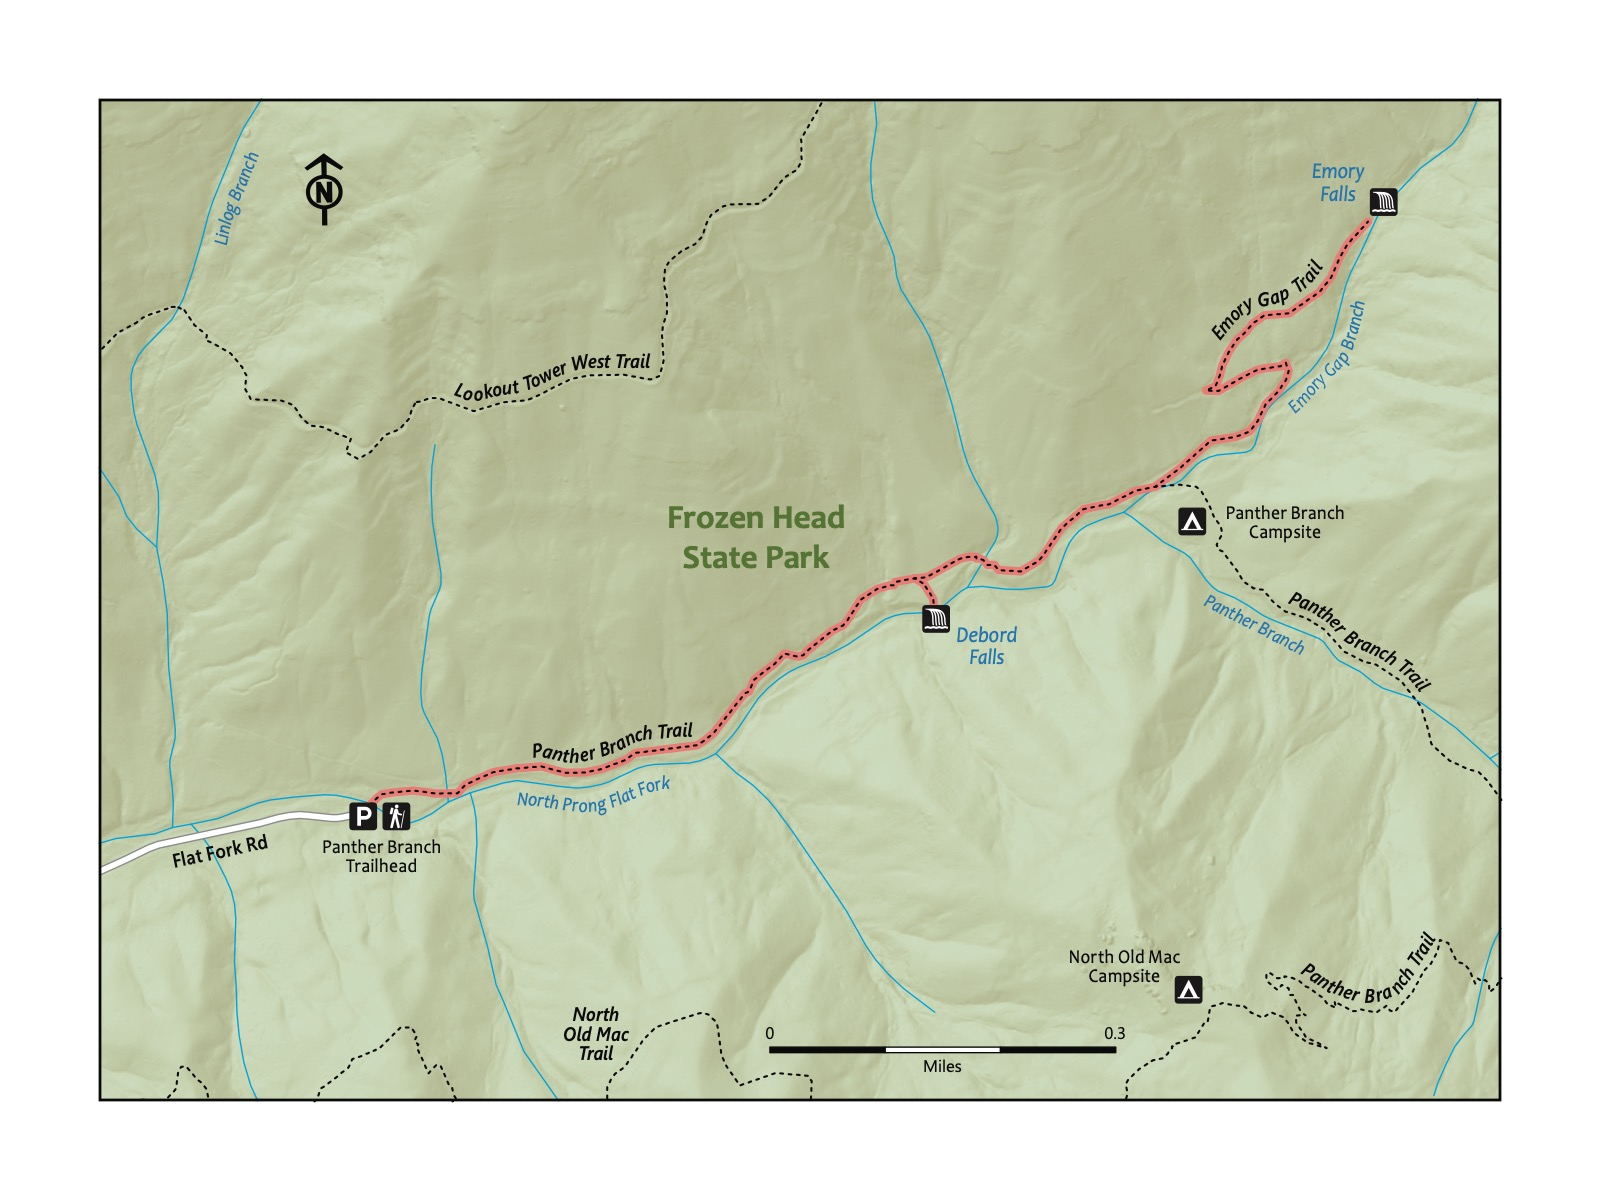
\includegraphics{maps/trail-13-map.jpeg}

\hypertarget{overview-12}{%
\subsubsection{Overview}\label{overview-12}}

Writing about this trail makes us smile. In many ways, it's the perfect
kid hike! It starts at a beautiful trailhead along a pretty creek in the
deep woods. It gradually climbs before stopping at a scenic waterfall,
DeBord Falls---one of two, and a perfectly acceptable place to turn
around with younger kids (we have many times). It continues further to
Emory Falls before returning on a gradual slope back to the trailhead.
Stop at the playground you passed on the way to the trailhead beside the
same creek; the water is usually shallow enough to be perfect for
splashing and rock hopping. Best for kids comfortable with rocky trails.

\includegraphics{img/trail-13-figure-01.jpg}

\hypertarget{directions-to-the-trailhead-12}{%
\subsubsection{Directions to the
Trailhead}\label{directions-to-the-trailhead-12}}

\begin{longtable}[]{@{}
  >{\raggedright\arraybackslash}p{(\columnwidth - 2\tabcolsep) * \real{0.3611}}
  >{\raggedright\arraybackslash}p{(\columnwidth - 2\tabcolsep) * \real{0.6389}}@{}}
\toprule\noalign{}
\begin{minipage}[b]{\linewidth}\raggedright
Trailhead Address
\end{minipage} & \begin{minipage}[b]{\linewidth}\raggedright
Emory Gap Trailhead, 4GP6+MV, Wartburg, TN 37887
\end{minipage} \\
\midrule\noalign{}
\endhead
\bottomrule\noalign{}
\endlastfoot
Trailhead GPS Coordinates & 36.13658, -84.48785 \\
\end{longtable}

:----- \textbar{}\\
\strut \\
\strut \\
Park in a spot at the Emory Gap Trailhead. Note that the above address
uses a ``Plus code'' that will only work in Google Maps---because Emory
Gap Trailhead does not have a street address. \textbar{}\\
\strut \\

\hypertarget{trail-description-12}{%
\subsubsection{Trail Description}\label{trail-description-12}}

\begin{longtable}[]{@{}
  >{\raggedright\arraybackslash}p{(\columnwidth - 2\tabcolsep) * \real{0.5000}}
  >{\raggedright\arraybackslash}p{(\columnwidth - 2\tabcolsep) * \real{0.5000}}@{}}
\toprule\noalign{}
\begin{minipage}[b]{\linewidth}\raggedright
Distance from Start
\end{minipage} & \begin{minipage}[b]{\linewidth}\raggedright
Description
\end{minipage} \\
\midrule\noalign{}
\endhead
\bottomrule\noalign{}
\endlastfoot
0.0 & Start by walking across the bridge at the trailhead. \\
0.55 & DeBord Falls. Walk down the stairs on the right to view the
waterfall from below. The trail continues along, but turn back if you
like (we often do!). \\
0.9 & Trail switchbacks. \\
1.1 & Steep and rocky section at the end to the viewing spot for Emory
Falls. \\
1.2 & After viewing the waterfall, head back to the start! \\
2.4 & Trailhead. \\
\end{longtable}

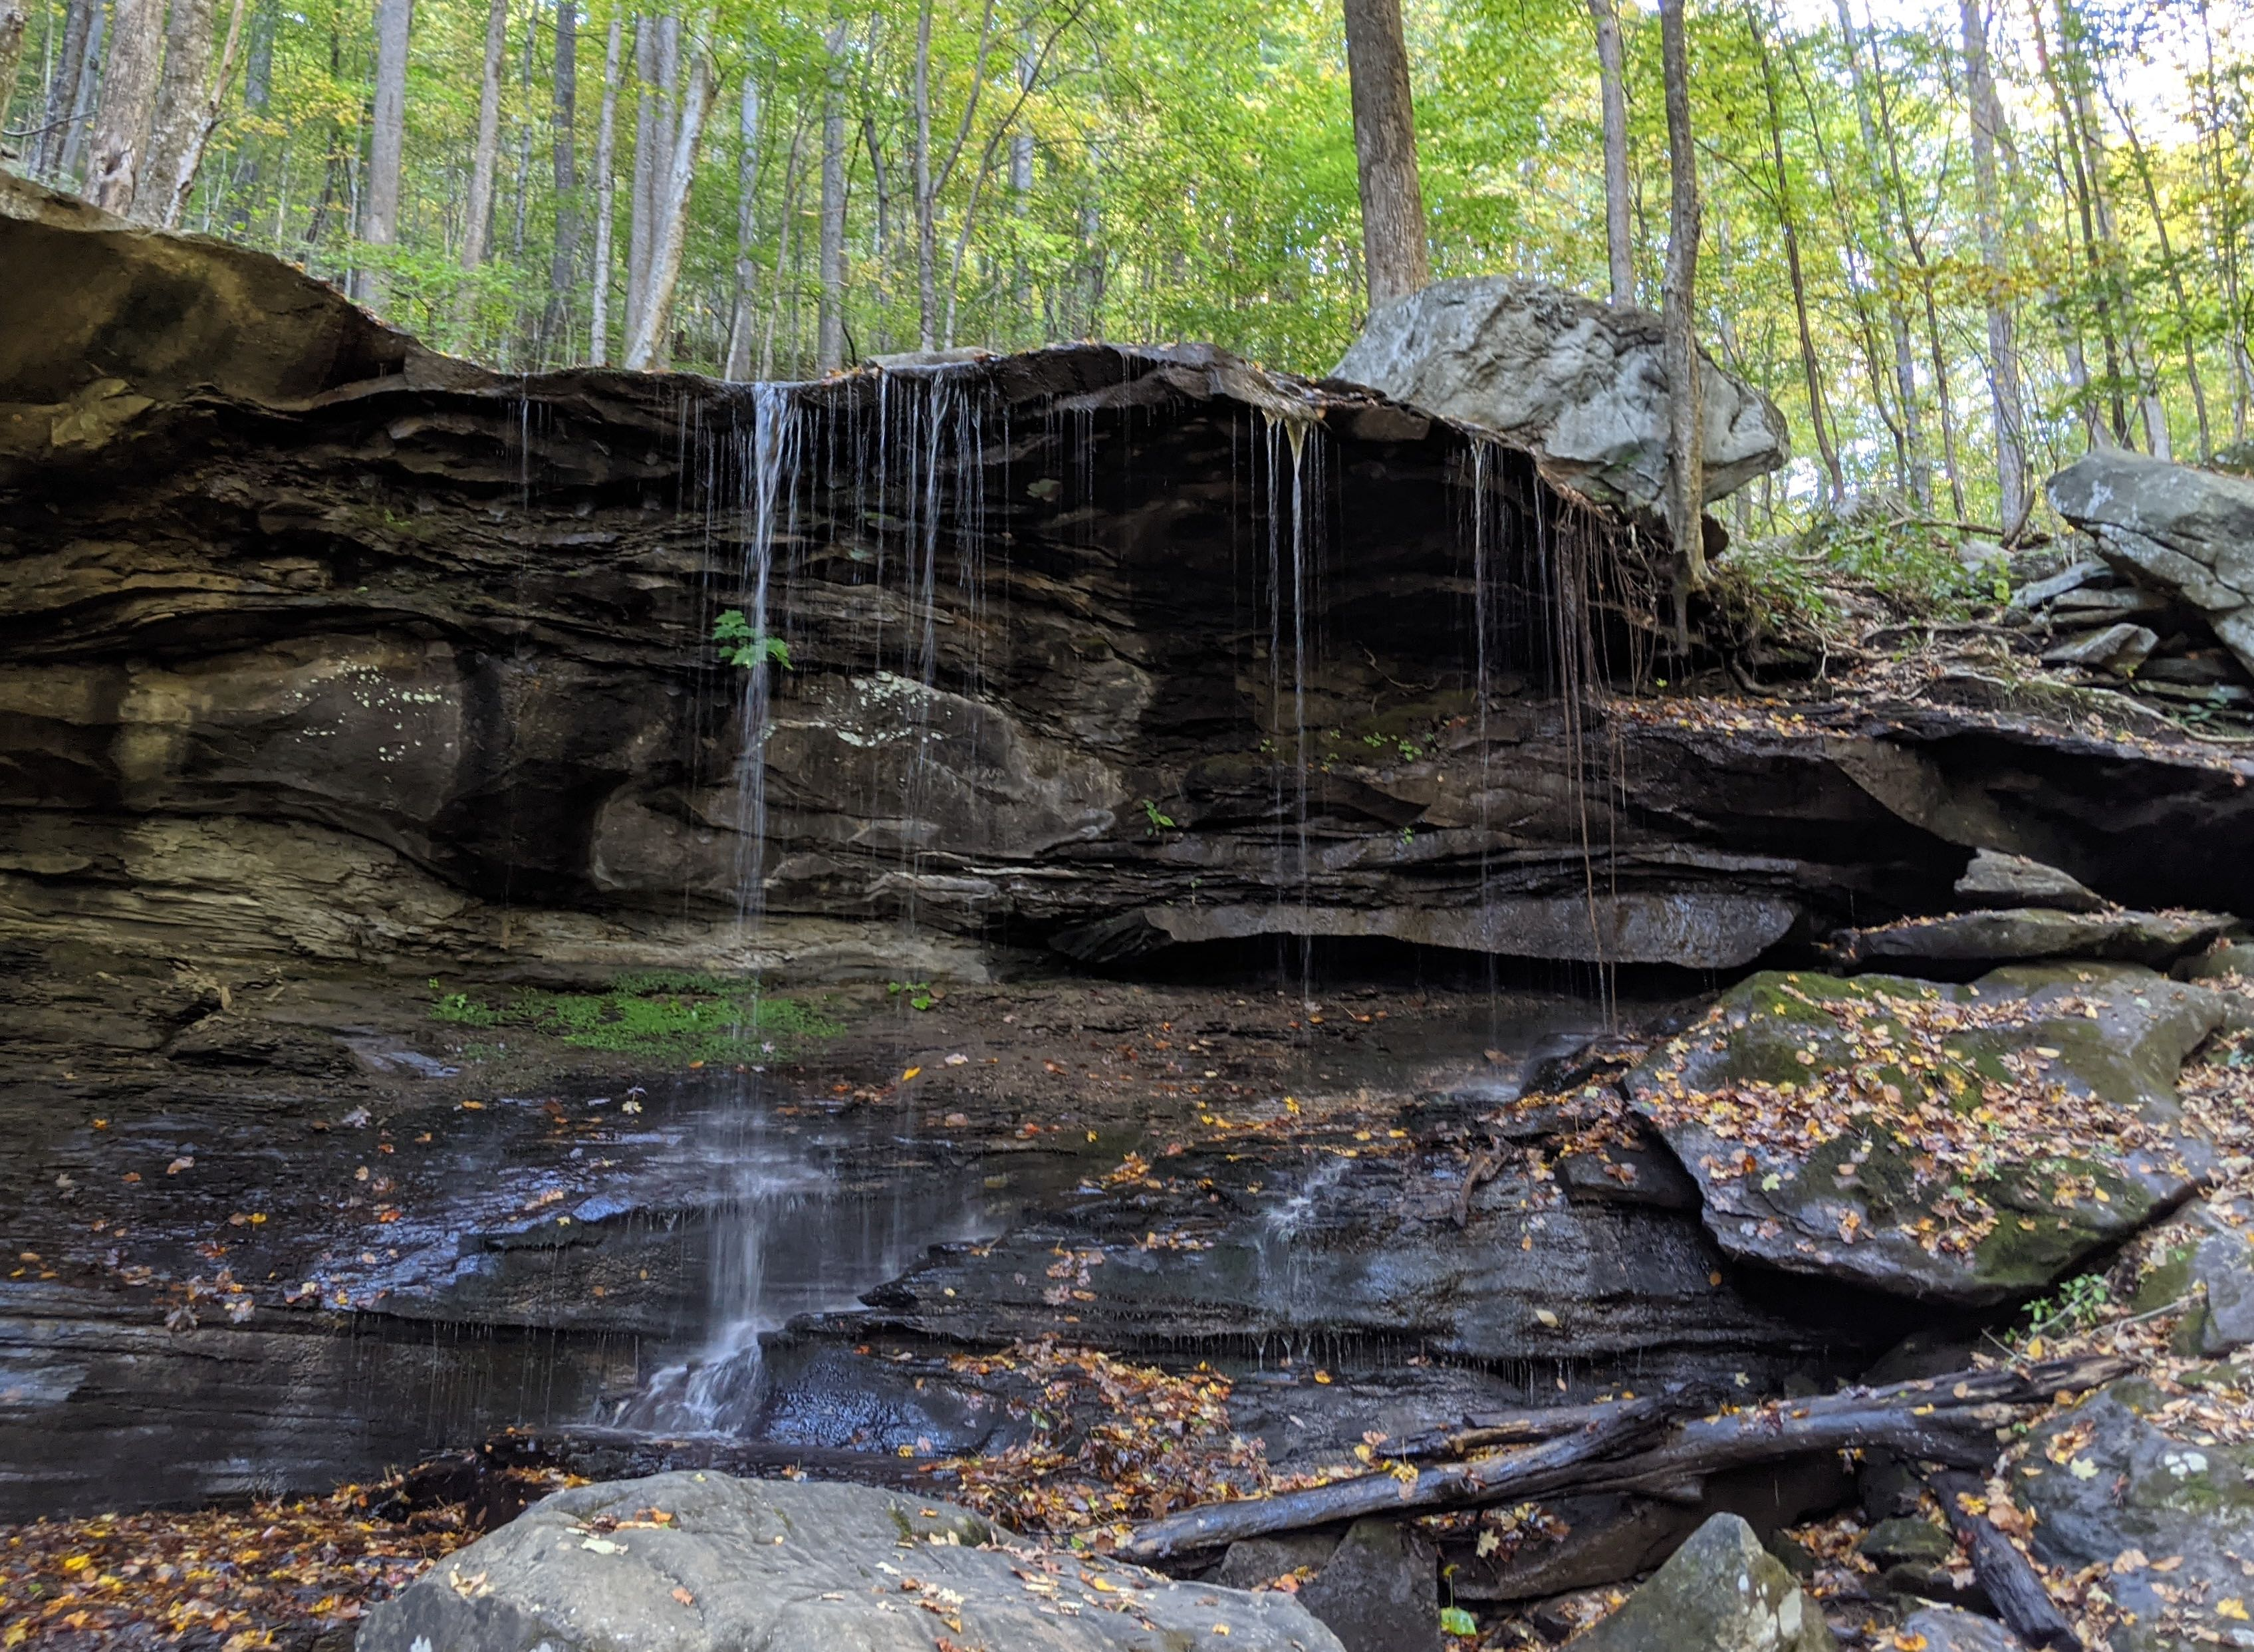
\includegraphics{img/trail-13-figure-02.jpg}

\hypertarget{nearby-12}{%
\subsubsection{Nearby}\label{nearby-12}}

\begin{itemize}
\tightlist
\item
  Playing at the playground. There is a fun, shaded creekside playground
  0.7 miles down the road from the trailhead; most of the year, the
  creek is a perfect depth for safe splashing.
\item
  Checking out the Flat Fork Story Book Trail. Starting near the
  playground, this short trail is great for the littlest hikers.
\item
  Hiking to the Frozen Head Mountain Summit. A challenge for the biggest
  hikers---including adults! This hike is around strenuous seven miles
  to and back from the Lookout Tower at the summit of Frozen Head
  Mountain, from which views of the Smokies far in the distance can be
  faintly visible on clear days.
\end{itemize}

\hypertarget{trail-14-obed-point}{%
\subsection{Trail 14: Obed Point}\label{trail-14-obed-point}}

\hypertarget{key-characteristics-13}{%
\subsubsection{Key Characteristics}\label{key-characteristics-13}}

\begin{longtable}[]{@{}ll@{}}
\toprule\noalign{}
Trail Name & Obed Point Trail \\
\midrule\noalign{}
\endhead
\bottomrule\noalign{}
\endlastfoot
Region & Cumberland Plateau \\
Trail \# & 14 \\
Time Estimate - Hiking Fast & 2.5 hours \\
Time Estimate - Hiking Slowly & 4.5 hours \\
Trail Distance (Miles) & 3.6 \\
Elevation Change & Gentle \\
Pets & Allowed on leash \\
Parking Pass/Entrance Fee & Not Required \\
Restroom(s) & Yes \\
Terrain & Dirt path \\
\end{longtable}

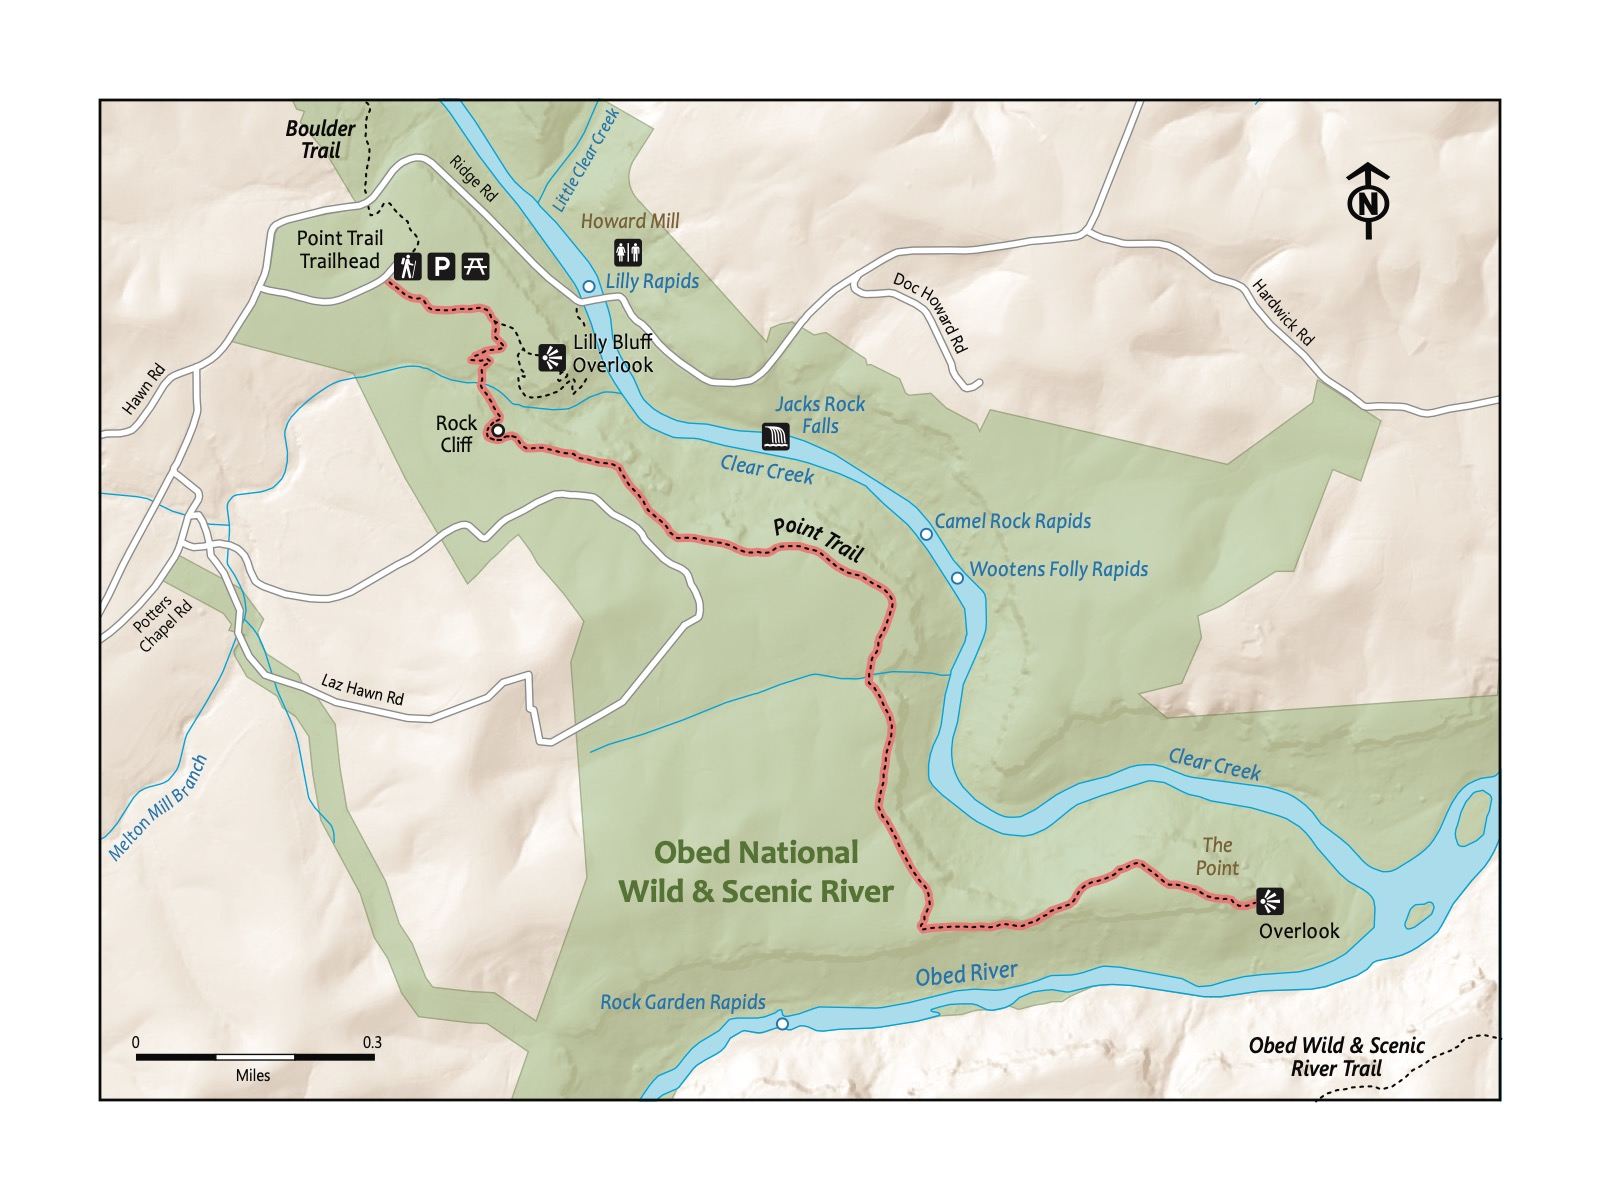
\includegraphics{maps/trail-14-map.jpeg}

\hypertarget{overview-13}{%
\subsubsection{Overview}\label{overview-13}}

Just far enough to be off the radar of many in Knoxville, this trail has
a bit of everything - fun bridge crossings, deep forest, waterfalls, and
two pretty overlooks. It does not climb so much as to become tiresome,
but it's long enough to feel like a real adventure. There's something
about the Obed area that feels both wild and inviting. The only
downside? It's a little out-of-the-way; in some ways, this trail feels
farther than some destinations in the Smokies. It's worth it for a great
family hike with kids of all ages. Though out of the way, there are a
few fun things to do to extend the hike or to visit very nearby on the
way home. Great for kids of all hiking ages, and not a bad hike on which
to carry a little one.

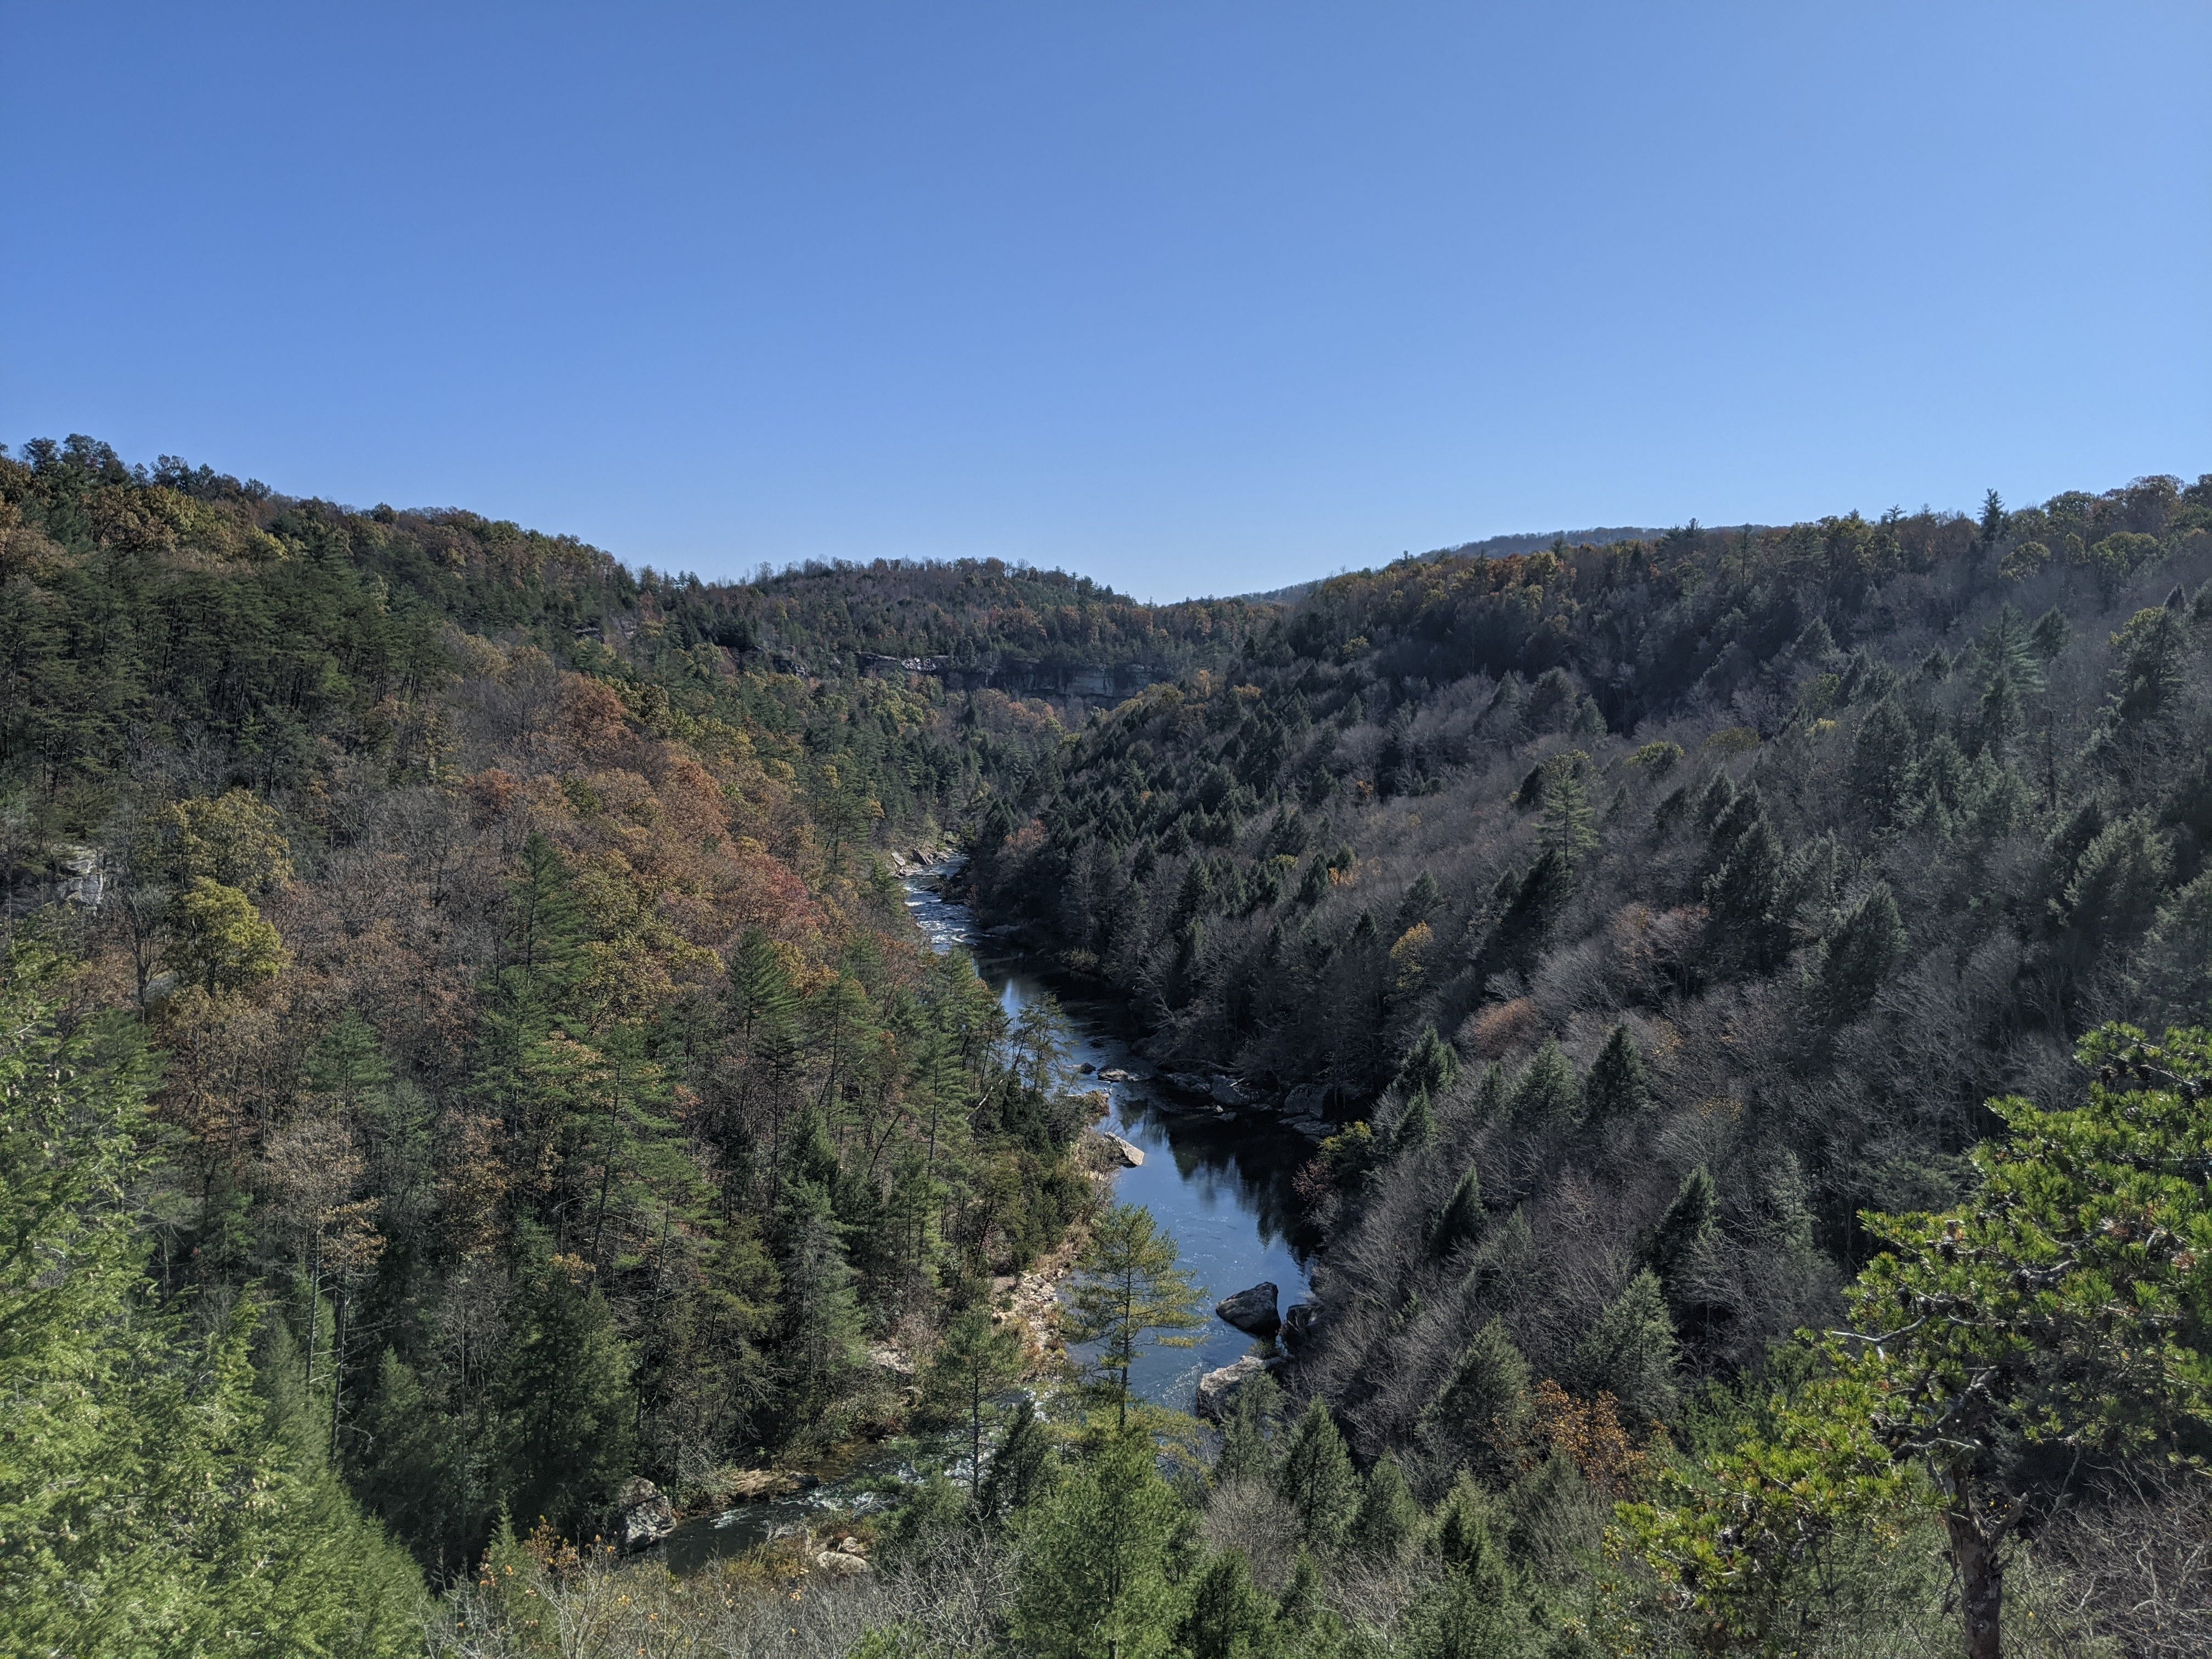
\includegraphics{img/trail-14-figure-01.jpg}

\hypertarget{directions-to-the-trailhead-13}{%
\subsubsection{Directions to the
Trailhead}\label{directions-to-the-trailhead-13}}

\begin{longtable}[]{@{}
  >{\raggedright\arraybackslash}p{(\columnwidth - 2\tabcolsep) * \real{0.5000}}
  >{\raggedright\arraybackslash}p{(\columnwidth - 2\tabcolsep) * \real{0.5000}}@{}}
\toprule\noalign{}
\begin{minipage}[b]{\linewidth}\raggedright
Trailhead Address
\end{minipage} & \begin{minipage}[b]{\linewidth}\raggedright
Lilly Bluff Trailhead, 1 Lilly Bluff Trail Head, Lancing, TN 37770
\end{minipage} \\
\midrule\noalign{}
\endhead
\bottomrule\noalign{}
\endlastfoot
Trailhead GPS Coordinates & 36.10239, -84.72183 \\
\end{longtable}

The above address should easily navigate you to the large parking area
with a restroom. Look for the sign for the point trail.

\hypertarget{trail-description-13}{%
\subsubsection{Trail Description}\label{trail-description-13}}

\begin{longtable}[]{@{}
  >{\raggedright\arraybackslash}p{(\columnwidth - 2\tabcolsep) * \real{0.5000}}
  >{\raggedright\arraybackslash}p{(\columnwidth - 2\tabcolsep) * \real{0.5000}}@{}}
\toprule\noalign{}
\begin{minipage}[b]{\linewidth}\raggedright
Distance from Start
\end{minipage} & \begin{minipage}[b]{\linewidth}\raggedright
Description
\end{minipage} \\
\midrule\noalign{}
\endhead
\bottomrule\noalign{}
\endlastfoot
0.0 & Start on the Point Trail. \\
0.15 & Side trial to the Lilly Bluff Overlook for Clear Freek ---
absolutely worth the short trip! \\
0.4 & Small bridge crossing. \\
0.45 & Large boulders and a rock wall --- the trail winds around the
side and atop the back of the wall. \\
0.5 & Trail flattens and winds along the side of a ridge. \\
1 & Trail bends to the right. \\
1.4 & Trail bends to the left. \\
1.8 & Overlook of the juncture of Clear Creek and Obed River. There
isn't really one overlook, per se, but many great spots to view the
rivers! After a good rest, turn around and head back to the
trailjhead. \\
3.6 & Trailhead. \\
\end{longtable}

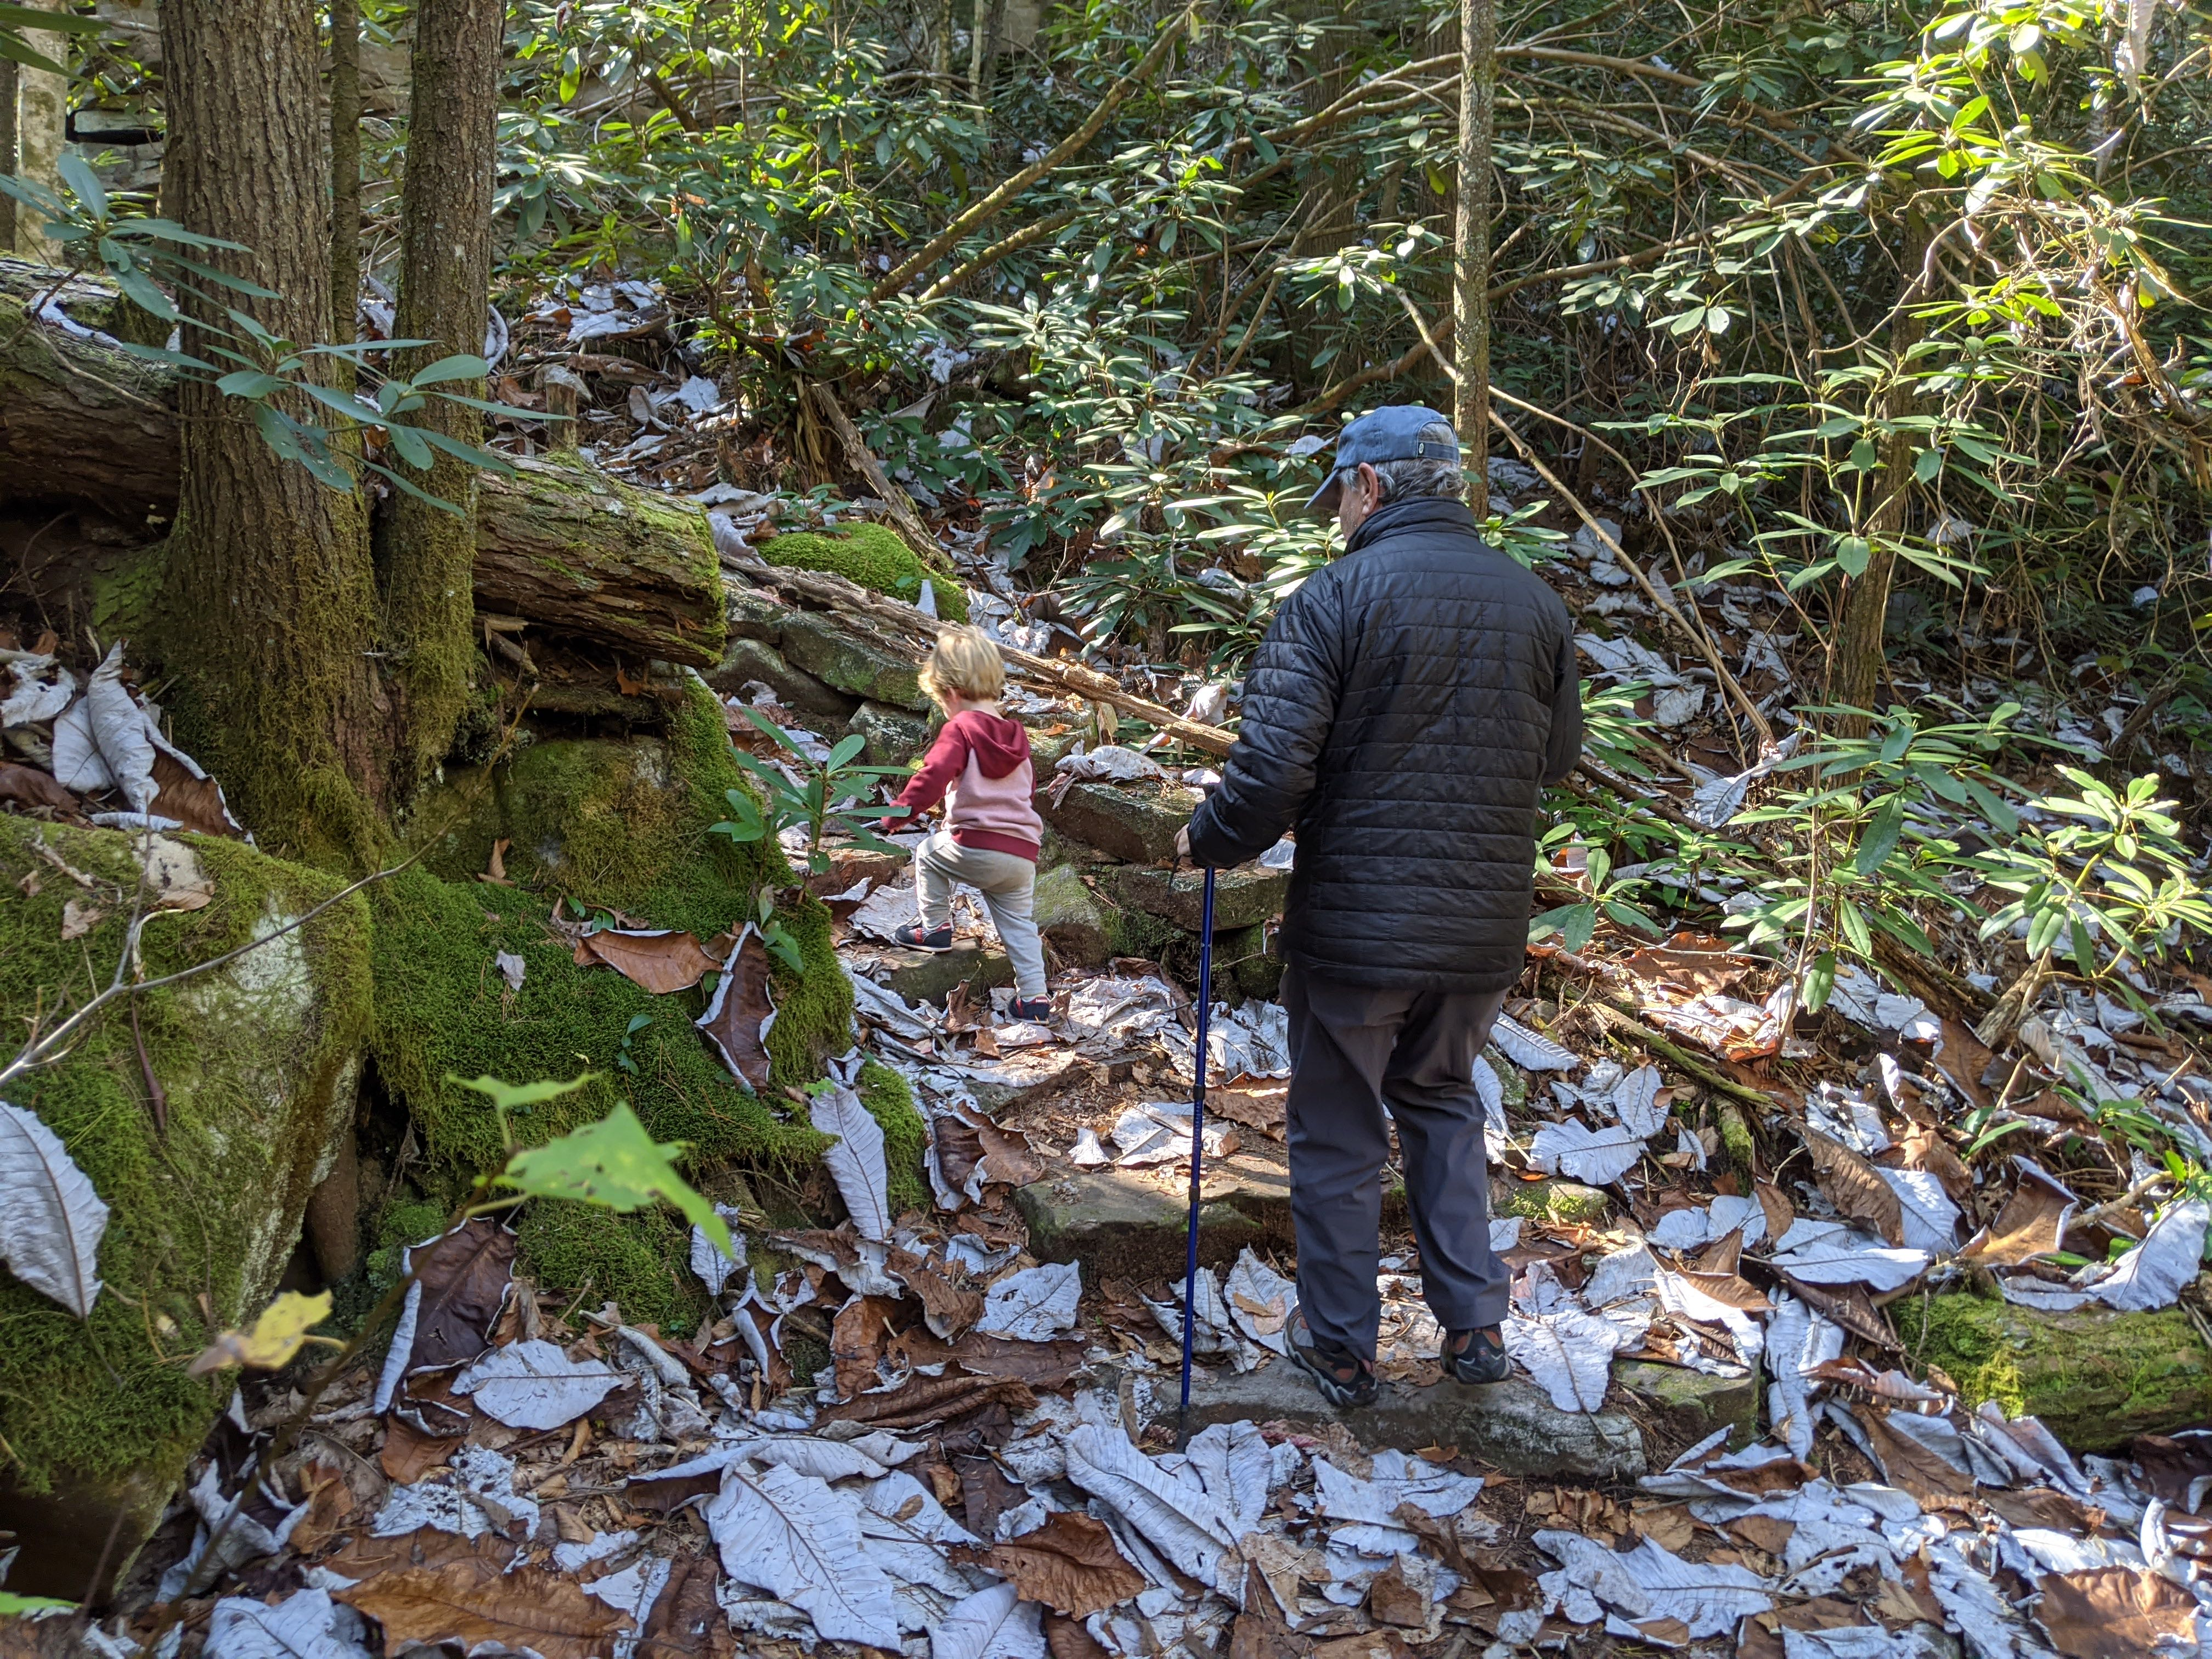
\includegraphics{img/trail-14-figure-02.jpg}

\hypertarget{nearby-13}{%
\subsubsection{Nearby}\label{nearby-13}}

\begin{itemize}
\tightlist
\item
  Hanging out at Lilly Pad Hopyard Brewery. Befitting the Obed Wild \&
  Scenic Area, the Lilly Pad Hopyard Brewery
  (\url{https://www.lillypadhopyardbrewery.com}) is a surprising,
  fantastic, kid-friendly destination. Stop by for food and
  drinks---only on Saturday and Sunday from 12-6 pm.
\item
  Playing around the bouldering area. The Trailhead features a nearby
  shaded area full of boulders. While we've often used this spot as a
  peaceful place to finish kiddo naps, older kids love trying to climb
  the boulders.
\end{itemize}

\hypertarget{trail-15-bandy-creek}{%
\subsection{Trail 15: Bandy Creek}\label{trail-15-bandy-creek}}

\hypertarget{key-characteristics-14}{%
\subsubsection{Key Characteristics}\label{key-characteristics-14}}

\begin{longtable}[]{@{}ll@{}}
\toprule\noalign{}
Trail Name & Bandy Creek \\
\midrule\noalign{}
\endhead
\bottomrule\noalign{}
\endlastfoot
Region & Cumberland Plateau \\
Trail \# & 15 \\
Time Estimate - Hiking Fast & 45 minutes \\
Time Estimate - Hiking Slowly & 1 hour, 15 minutes \\
Trail Distance (Miles) & 1.3 \\
Elevation Change & Flat \\
Pets & Allowed on leash \\
Parking Pass/Entrance Fee & Not Required \\
Restroom(s) & Yes \\
Terrain & Dirt path \\
\end{longtable}

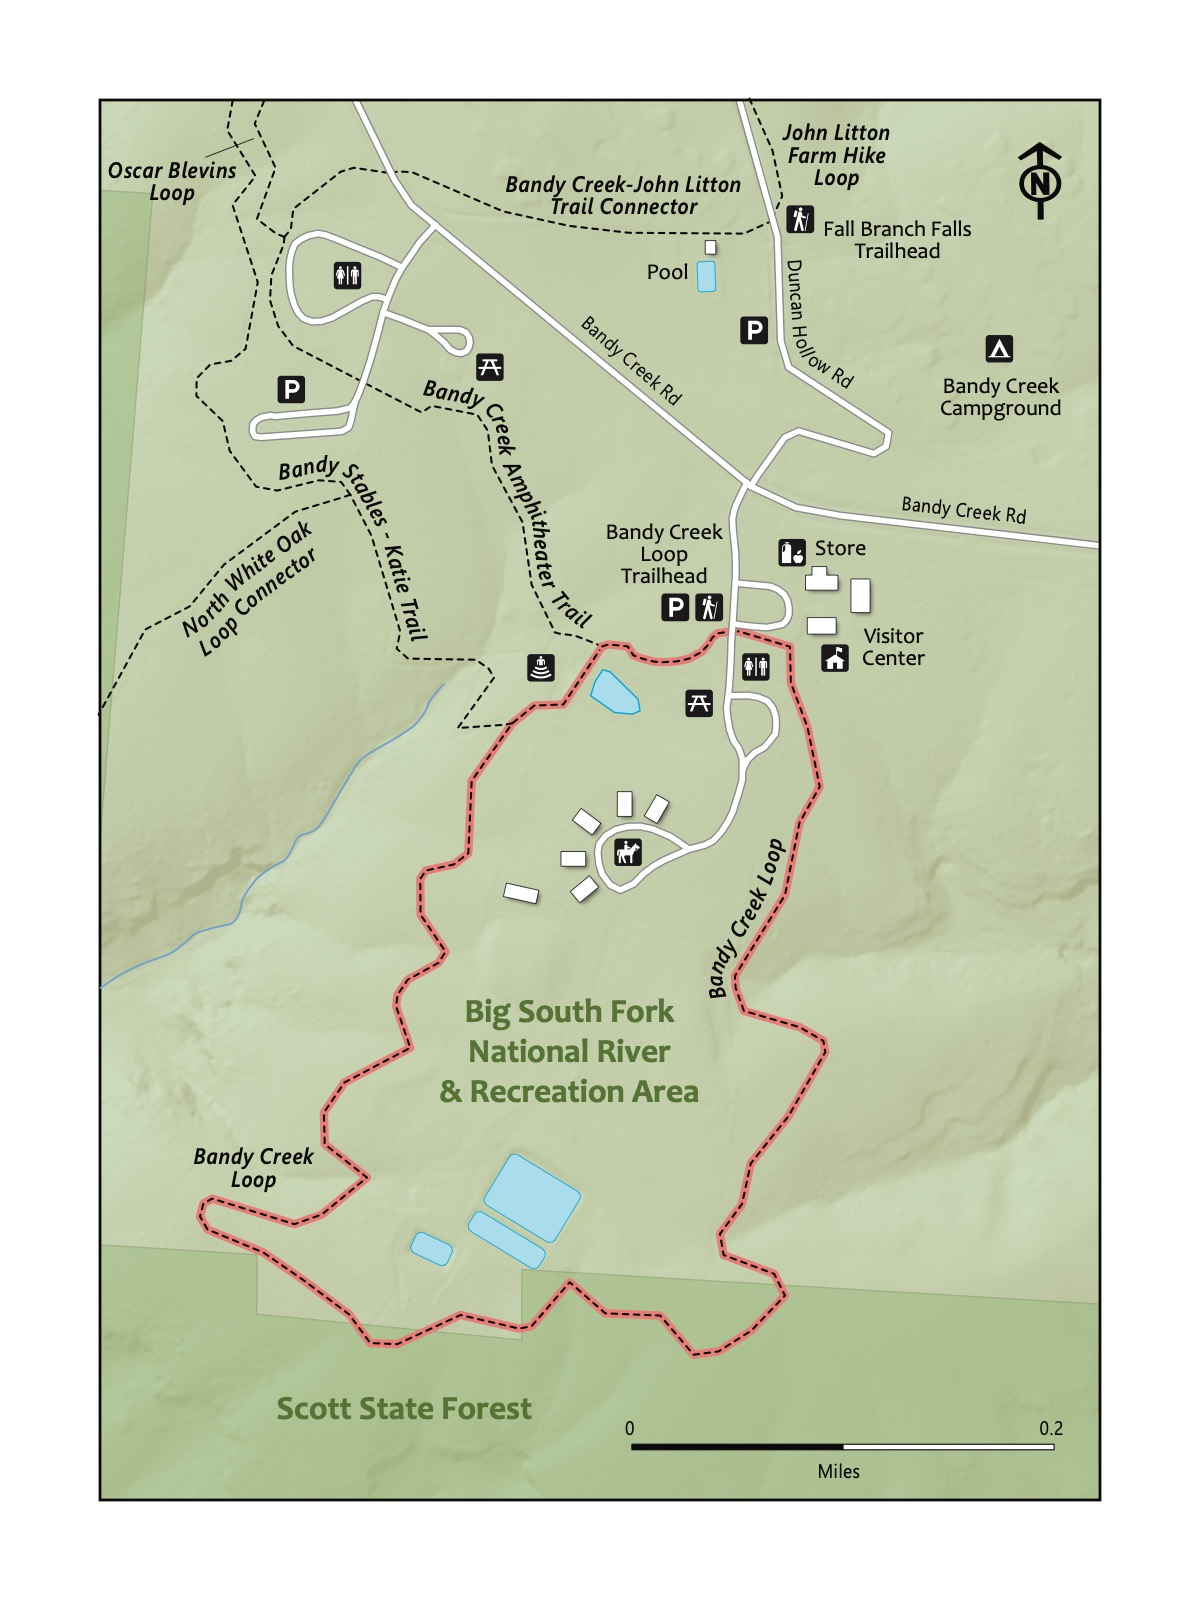
\includegraphics{maps/trail-15-map.jpeg}

\hypertarget{overview-14}{%
\subsubsection{Overview}\label{overview-14}}

A welcoming, gentle introduction to the Big South Fork. Best if you're
staying at the campground -- or if you're hiking the nearby Angel Falls
Trail or the Fall Branch Falls trails. Starts at the visitor center.
This happens to be the flattest trail in the book, and it's a short
trail, but it's almost entirely on a dirt path. This is a great hike for
toddlers or little kids, and it is good for carried infants.

{[}PLACEHOLDER -
CHANGE{]}{[}/img/trail-15-figure-01-placeholder-dont-use.png{]}

\hypertarget{directions-to-the-trailhead-14}{%
\subsubsection{Directions to the
Trailhead}\label{directions-to-the-trailhead-14}}

\begin{longtable}[]{@{}
  >{\raggedright\arraybackslash}p{(\columnwidth - 2\tabcolsep) * \real{0.5000}}
  >{\raggedright\arraybackslash}p{(\columnwidth - 2\tabcolsep) * \real{0.5000}}@{}}
\toprule\noalign{}
\begin{minipage}[b]{\linewidth}\raggedright
Trailhead Address
\end{minipage} & \begin{minipage}[b]{\linewidth}\raggedright
Bandy Creek Visitors Center, 151 Stable Rd, Oneida, TN 37841
\end{minipage} \\
\midrule\noalign{}
\endhead
\bottomrule\noalign{}
\endlastfoot
Trailhead GPS Coordinates & 36.49062, -84.69777 \\
\end{longtable}

The trailhead address will navigate you to the nearby Visitors Center
(worth a visit when open---9:00 am - 5:00 pm year-round!). From the
Visitors Center, look for the signs for the Bandy Creek Loop to begin
the hike.

\hypertarget{trail-description-14}{%
\subsubsection{Trail Description}\label{trail-description-14}}

\begin{longtable}[]{@{}
  >{\raggedright\arraybackslash}p{(\columnwidth - 2\tabcolsep) * \real{0.5000}}
  >{\raggedright\arraybackslash}p{(\columnwidth - 2\tabcolsep) * \real{0.5000}}@{}}
\toprule\noalign{}
\begin{minipage}[b]{\linewidth}\raggedright
Distance from Start
\end{minipage} & \begin{minipage}[b]{\linewidth}\raggedright
Description
\end{minipage} \\
\midrule\noalign{}
\endhead
\bottomrule\noalign{}
\endlastfoot
0.0 & Start on the Bandy Loop Trail. Wind gradually toward the horse
stables. \\
0.15 & Pass the horse stables on the right. There's an easy connector
trail to them nearer the end of the loop. \\
1.15 & Connector trail to the horse stables. \\
1.3 & Return to the parking area and trailhead. \\
\end{longtable}

\hypertarget{nearby-14}{%
\subsubsection{Nearby}\label{nearby-14}}

\begin{itemize}
\tightlist
\item
  Visiting the horse stables. Kids will likely love the nearby stables
  that often house many horses ---most from guests at the campground who
  will ride the trails that allow horses. The nearby Bandy Creek Loop
  trail is also a good, short hike for young kiddos.
\item
  Camping at Bandy Creek. This is a large, modern, scenic campground,
  very much worth a visit, though it is off-the-radar of many. You can
  almost always find a spot here --- even on holiday weekends.
\item
  Hiking the Fall Branch Falls or Angel Falls trails. See those chapters
  for more details.
\end{itemize}

\hypertarget{trail-16-fall-branch-falls}{%
\subsection{Trail 16: Fall Branch
Falls}\label{trail-16-fall-branch-falls}}

\hypertarget{key-characteristics-15}{%
\subsubsection{Key Characteristics}\label{key-characteristics-15}}

\begin{longtable}[]{@{}ll@{}}
\toprule\noalign{}
Trail Name & Fall Branch Falls \\
\midrule\noalign{}
\endhead
\bottomrule\noalign{}
\endlastfoot
Region & Cumberland Plateau \\
Trail \# & 15 \\
Time Estimate - Hiking Fast & 2.5 hours \\
Time Estimate - Hiking Slowly & 4.5 hours \\
Trail Distance (Miles) & 3.7 \\
Elevation Change & Moderate \\
Pets & Allowed on leash \\
Parking Pass/Entrance Fee & Not Required \\
Restroom(s) & Yes \\
Terrain & Dirt path; ladders; rocky path \\
\end{longtable}

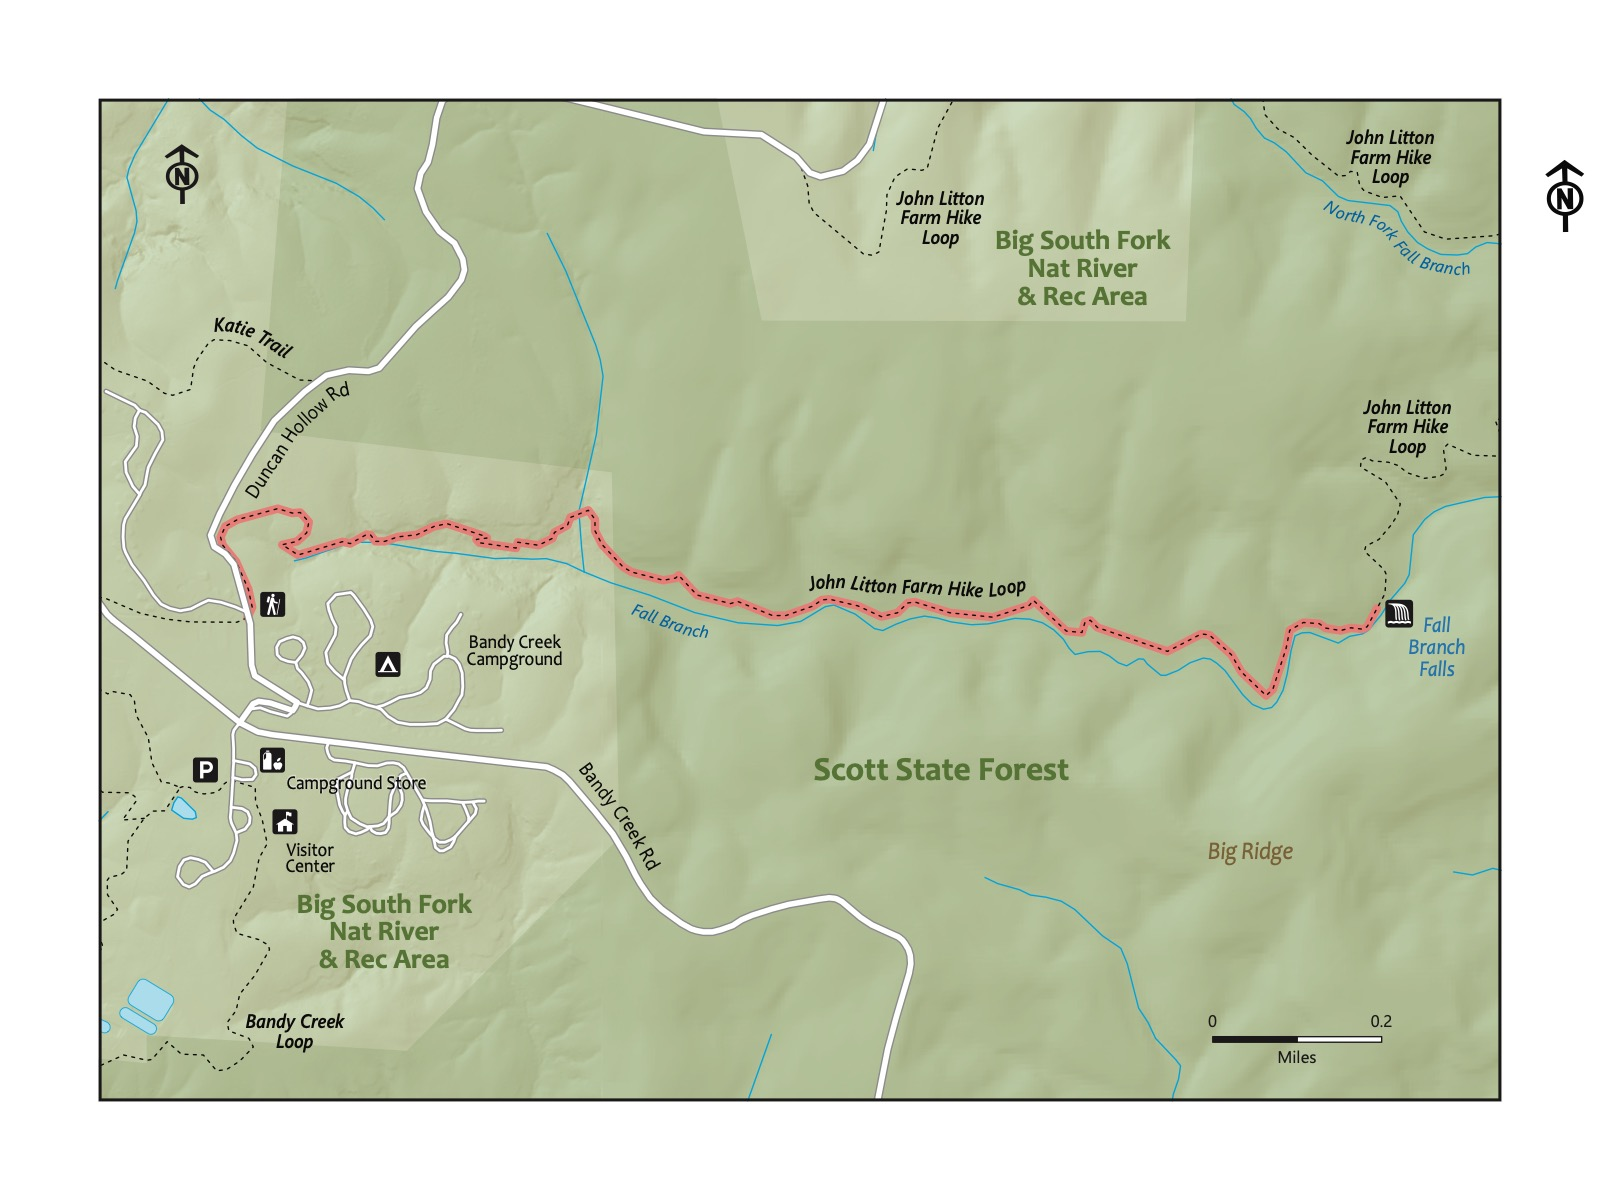
\includegraphics{maps/trail-16-map.jpeg}

\hypertarget{overview-15}{%
\subsubsection{Overview}\label{overview-15}}

Part of the Big South Fork National River and Recreation Area, a
National Park Service-administered area that is a perfect counterbalance
to the wonderful but far more familiar Great Smoky Mountains National
Park. This hike, like the Big South Fork, is quieter and subtler than
the Smokies. It features unique rock cliffs that are perfect for kids to
ogle and explore. The visitor center, horse stables---not to mention
100s of miles of nearby trails, complement the hike. Because you can
turn around at any point, suitable for kids of any ages. Just be aware
of the ladders that can be a little tricky for the youngest kids to
navigate!

{[}Credit to VioletSkyAdventures (photo 2487905531 on
Shutterstock){]}{[}/img/trail-16-figure-01.jpg{]}

\hypertarget{directions-to-the-trailhead-15}{%
\subsubsection{Directions to the
Trailhead}\label{directions-to-the-trailhead-15}}

\begin{longtable}[]{@{}
  >{\raggedright\arraybackslash}p{(\columnwidth - 2\tabcolsep) * \real{0.5000}}
  >{\raggedright\arraybackslash}p{(\columnwidth - 2\tabcolsep) * \real{0.5000}}@{}}
\toprule\noalign{}
\begin{minipage}[b]{\linewidth}\raggedright
Trailhead Address
\end{minipage} & \begin{minipage}[b]{\linewidth}\raggedright
Bandy Creek Visitors Center, 151 Stable Rd, Oneida, TN 37841
\end{minipage} \\
\midrule\noalign{}
\endhead
\bottomrule\noalign{}
\endlastfoot
Trailhead GPS Coordinates & 36.49062, -84.69777 \\
\end{longtable}

The trailhead address will navigate you to the nearby Visitors Center
(worth a visit when open---9:00 am - 5:00 pm year-round!). From the
Visitors Center, walk across Bandy Loop Road toward the campground. Find
Duncan Hollow Road, and walk up it a short distance, passing the Bandy
Creek Pool (at which you could also park) on the left. The trailhead is
immediately past the pool on the right side of Duncan Hollow Road.

\hypertarget{trail-description-15}{%
\subsubsection{Trail Description}\label{trail-description-15}}

\begin{longtable}[]{@{}
  >{\raggedright\arraybackslash}p{(\columnwidth - 2\tabcolsep) * \real{0.5000}}
  >{\raggedright\arraybackslash}p{(\columnwidth - 2\tabcolsep) * \real{0.5000}}@{}}
\toprule\noalign{}
\begin{minipage}[b]{\linewidth}\raggedright
Distance from Start
\end{minipage} & \begin{minipage}[b]{\linewidth}\raggedright
Description
\end{minipage} \\
\midrule\noalign{}
\endhead
\bottomrule\noalign{}
\endlastfoot
0.0 & Start on the Litten-Slaven Farm Loop Trail. \\
0.2 & Begin to gradually descend into the Fall Branch creekbed. \\
0.5 & Trail levels. \\
0.55 & Rocky section featuring a short ladder (to make it easier to
navigate through the rocks). \\
1.8 & Fall Branch Falls. A great spot for a break before turning around
to return to the start. \\
3.6 & Trailhead. \\
\end{longtable}

\hypertarget{nearby-15}{%
\subsubsection{Nearby}\label{nearby-15}}

\begin{itemize}
\tightlist
\item
  Camping at Bandy Creek! The Bandy Creek Campground is a gem - spacious
  sites, nice restrooms, and lots of cul-de-sacs for kids to endlessly
  play or bike. Consider a stay here as a launching point for this hike.
\item
  Stopping by the visitor's center. A good place to learn more about the
  Big South Fork---and to ask any questions or to seek the advice of
  park rangers.
\item
  Hiking the nearby Bandy Creek or Angel Falls Trails. Check out the
  Bandy Creek or Angel Falls Trails chapters. Note there are 100s of
  miles of other trails in this area, many well worth a hike (the Grand
  Gap Loop is a lengthy favorite!). Consider stopping the the visitor
  center to ask for recommendations and up-to-date information.
\end{itemize}

\hypertarget{trail-17-twin-arches}{%
\subsection{Trail 17: Twin Arches}\label{trail-17-twin-arches}}

\hypertarget{key-characteristics-16}{%
\subsubsection{Key Characteristics}\label{key-characteristics-16}}

\begin{longtable}[]{@{}ll@{}}
\toprule\noalign{}
Trail Name & Twin Arches Loop \\
\midrule\noalign{}
\endhead
\bottomrule\noalign{}
\endlastfoot
Region & Cumberland Plateau \\
Trail \# & 16 \\
Time Estimate - Hiking Fast & 1.5 hour \\
Time Estimate - Hiking Slowly & 2.5 hours \\
Trail Distance (Miles) & 1.2 \\
Elevation Change & Moderate \\
Pets & Allowed on leash \\
Parking Pass/Entrance Fee & Not Required \\
Restroom(s) & Yes \\
Terrain & Dirt path; stairs \\
\end{longtable}

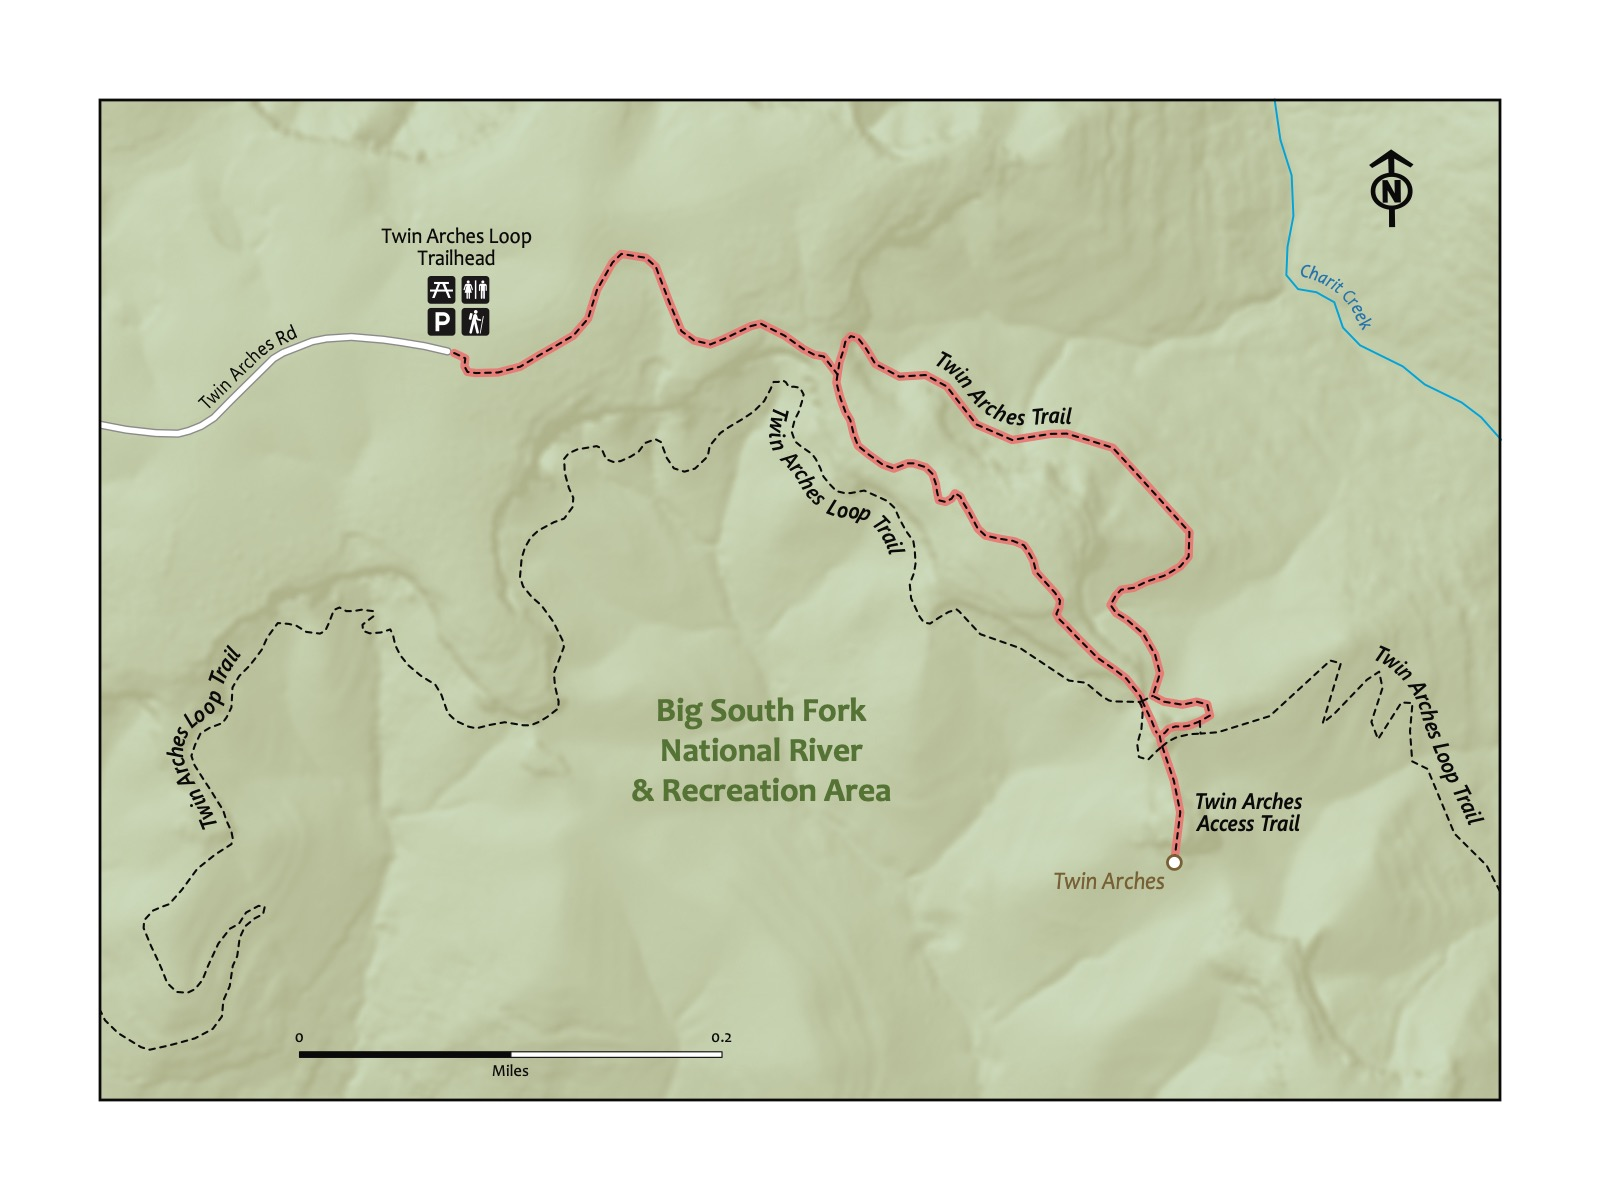
\includegraphics{maps/trail-17-map.jpeg}

\hypertarget{overview-16}{%
\subsubsection{Overview}\label{overview-16}}

This short hike leads to one of the most surprising geologic features in
Tennessee---the Twin Arches, a 130-foot span and 100-foot height feature
you can walk over, around, and through. The surrounding forest is not
shabby, either. This is a fantastic and memorable family hike, with some
challenges sprinkled in. First, this hike is the farthest (by driving
distance) of any in this book. Second, there are some rocky sections
that require some carefulness. Still, this is a must-see, and it's near
many features (and places to camp) to make a visit more accommodating.
Good for families with children of any walking age.

\includegraphics{img/trail-16-figure-01-1.jpg}

\hypertarget{directions-to-the-trailhead-16}{%
\subsubsection{Directions to the
Trailhead}\label{directions-to-the-trailhead-16}}

\begin{longtable}[]{@{}
  >{\raggedright\arraybackslash}p{(\columnwidth - 2\tabcolsep) * \real{0.5000}}
  >{\raggedright\arraybackslash}p{(\columnwidth - 2\tabcolsep) * \real{0.5000}}@{}}
\toprule\noalign{}
\begin{minipage}[b]{\linewidth}\raggedright
Trailhead Address
\end{minipage} & \begin{minipage}[b]{\linewidth}\raggedright
Twin Arches Trailhead, G7V5+Q7 Jamestown, Tennessee
\end{minipage} \\
\midrule\noalign{}
\endhead
\bottomrule\noalign{}
\endlastfoot
Trailhead GPS Coordinates & 36.48797, -84.69744 \\
\end{longtable}

The above address should easily navigate you to the large parking area
with a restroom. Note that the above address uses a Google Maps ``Plus
code'', as the trailhead does not have a street address. This will only
work in Google Maps.

Park, and look for the sign for the Twin Arches trail near the back of
the parking lot.

\hypertarget{trail-description-16}{%
\subsubsection{Trail Description}\label{trail-description-16}}

\begin{longtable}[]{@{}
  >{\raggedright\arraybackslash}p{(\columnwidth - 2\tabcolsep) * \real{0.5000}}
  >{\raggedright\arraybackslash}p{(\columnwidth - 2\tabcolsep) * \real{0.5000}}@{}}
\toprule\noalign{}
\begin{minipage}[b]{\linewidth}\raggedright
Distance from Start
\end{minipage} & \begin{minipage}[b]{\linewidth}\raggedright
Description
\end{minipage} \\
\midrule\noalign{}
\endhead
\bottomrule\noalign{}
\endlastfoot
0.0 & Start on the Twin Arches trail. \\
0.25 & Intersection. Head right to complete the loop in a
counterclockwise section (though, it is perfectly fine to head in the
other direction!). \\
0.3 & Stairs. \\
0.5 & Arrive at the base of the Twin Arches. Head straight - you won't
be able to miss them! \\
0.6 & Twin Arches. Walk along the top of the arches, under them, and
around them, and then head back toward the loop portion of the trail. \\
0.7 & Turn right at the intersection to complete the counterclockwise
loop. \\
0.95 & Intersection. Turn right to return to the trailhead. \\
1.20 & Trailhead. \\
\end{longtable}

\hypertarget{nearby-16}{%
\subsubsection{Nearby}\label{nearby-16}}

\begin{itemize}
\tightlist
\item
  Camping or renting a cabin at Pickett State Park. Pickett State Park,
  a nice campground that also has both historic and modern cabins to
  rent, is close to this trail. It also features a great lake for
  kayaking, canoeing, or paddle boarding.
\item
  View the night sky. Pickett State Park has a Silver-tier designation
  as an International Dark Sky Park. Even if you're not strictly in the
  State Park, this is a great place to view stars and planets in the
  night sky.
\end{itemize}

\hypertarget{trail-18-angel-falls}{%
\subsection{Trail 18: Angel Falls}\label{trail-18-angel-falls}}

\hypertarget{key-characteristics-17}{%
\subsubsection{Key Characteristics}\label{key-characteristics-17}}

\begin{longtable}[]{@{}ll@{}}
\toprule\noalign{}
Trail Name & Angel Falls Overlook \\
\midrule\noalign{}
\endhead
\bottomrule\noalign{}
\endlastfoot
Region & Cumberland Plateau \\
Trail \# & 17 \\
Time Estimate - Hiking Fast & 1.5 hours \\
Time Estimate - Hiking Slowly & 2.5 hours \\
Trail Distance (Miles) & 2.8 \\
Elevation Change & Gentle \\
Pets & Allowed on leash \\
Parking Pass/Entrance Fee & Not Required \\
Restroom(s) & No \\
Terrain & Dirt path \\
\end{longtable}

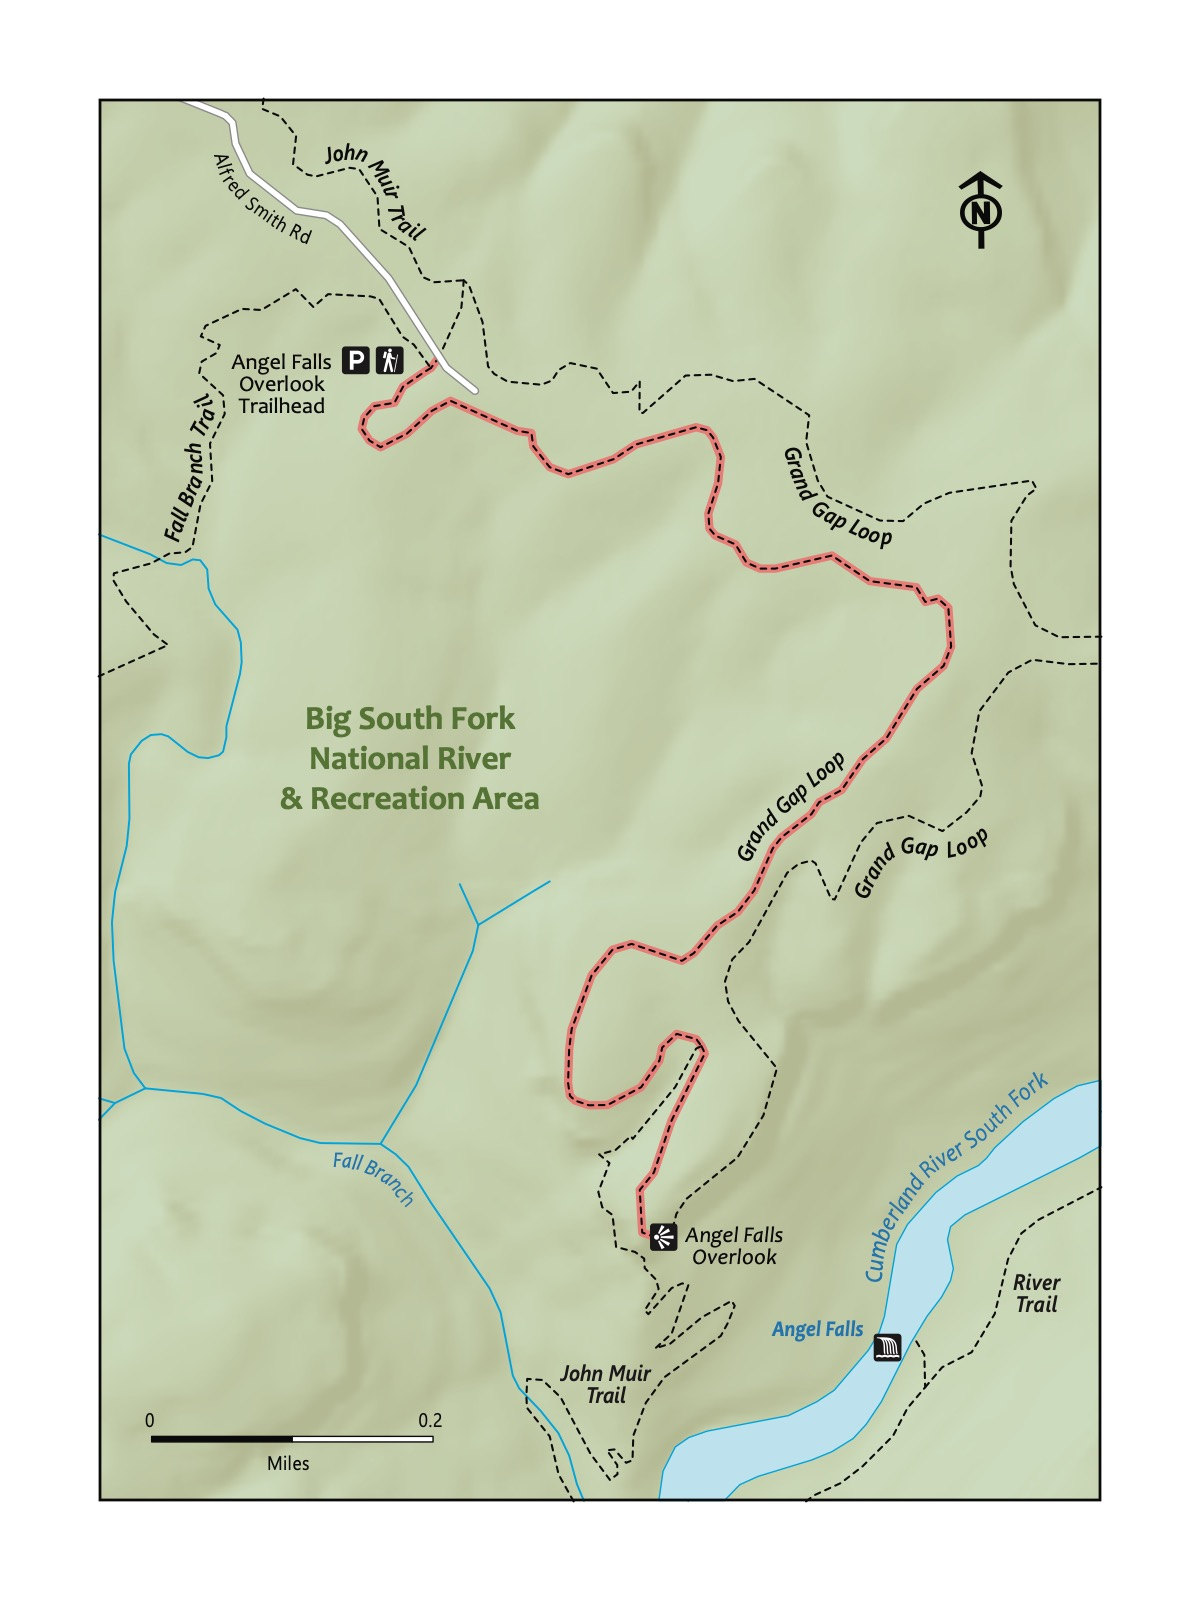
\includegraphics{maps/trail-18-map.jpeg}

\hypertarget{overview-17}{%
\subsubsection{Overview}\label{overview-17}}

Like a few of the other trails in or near the Cumberland Plateau, this
is a spectacular hike that is a little off-the-radar of many in
Knoxville. This is a spectacular hike that is a little tricky to get to
for a day hike. Still, the view is awesome, rivaling the summits of the
Smokies with a different kind of vantage --- here, of the beautiful Big
South Fork River. This trail is relatively flat and relatively short,
making it appropriate for families with young children. Consider camping
at the nearby Bandy Creek campground, and consider this hike a day's
excursion from there.

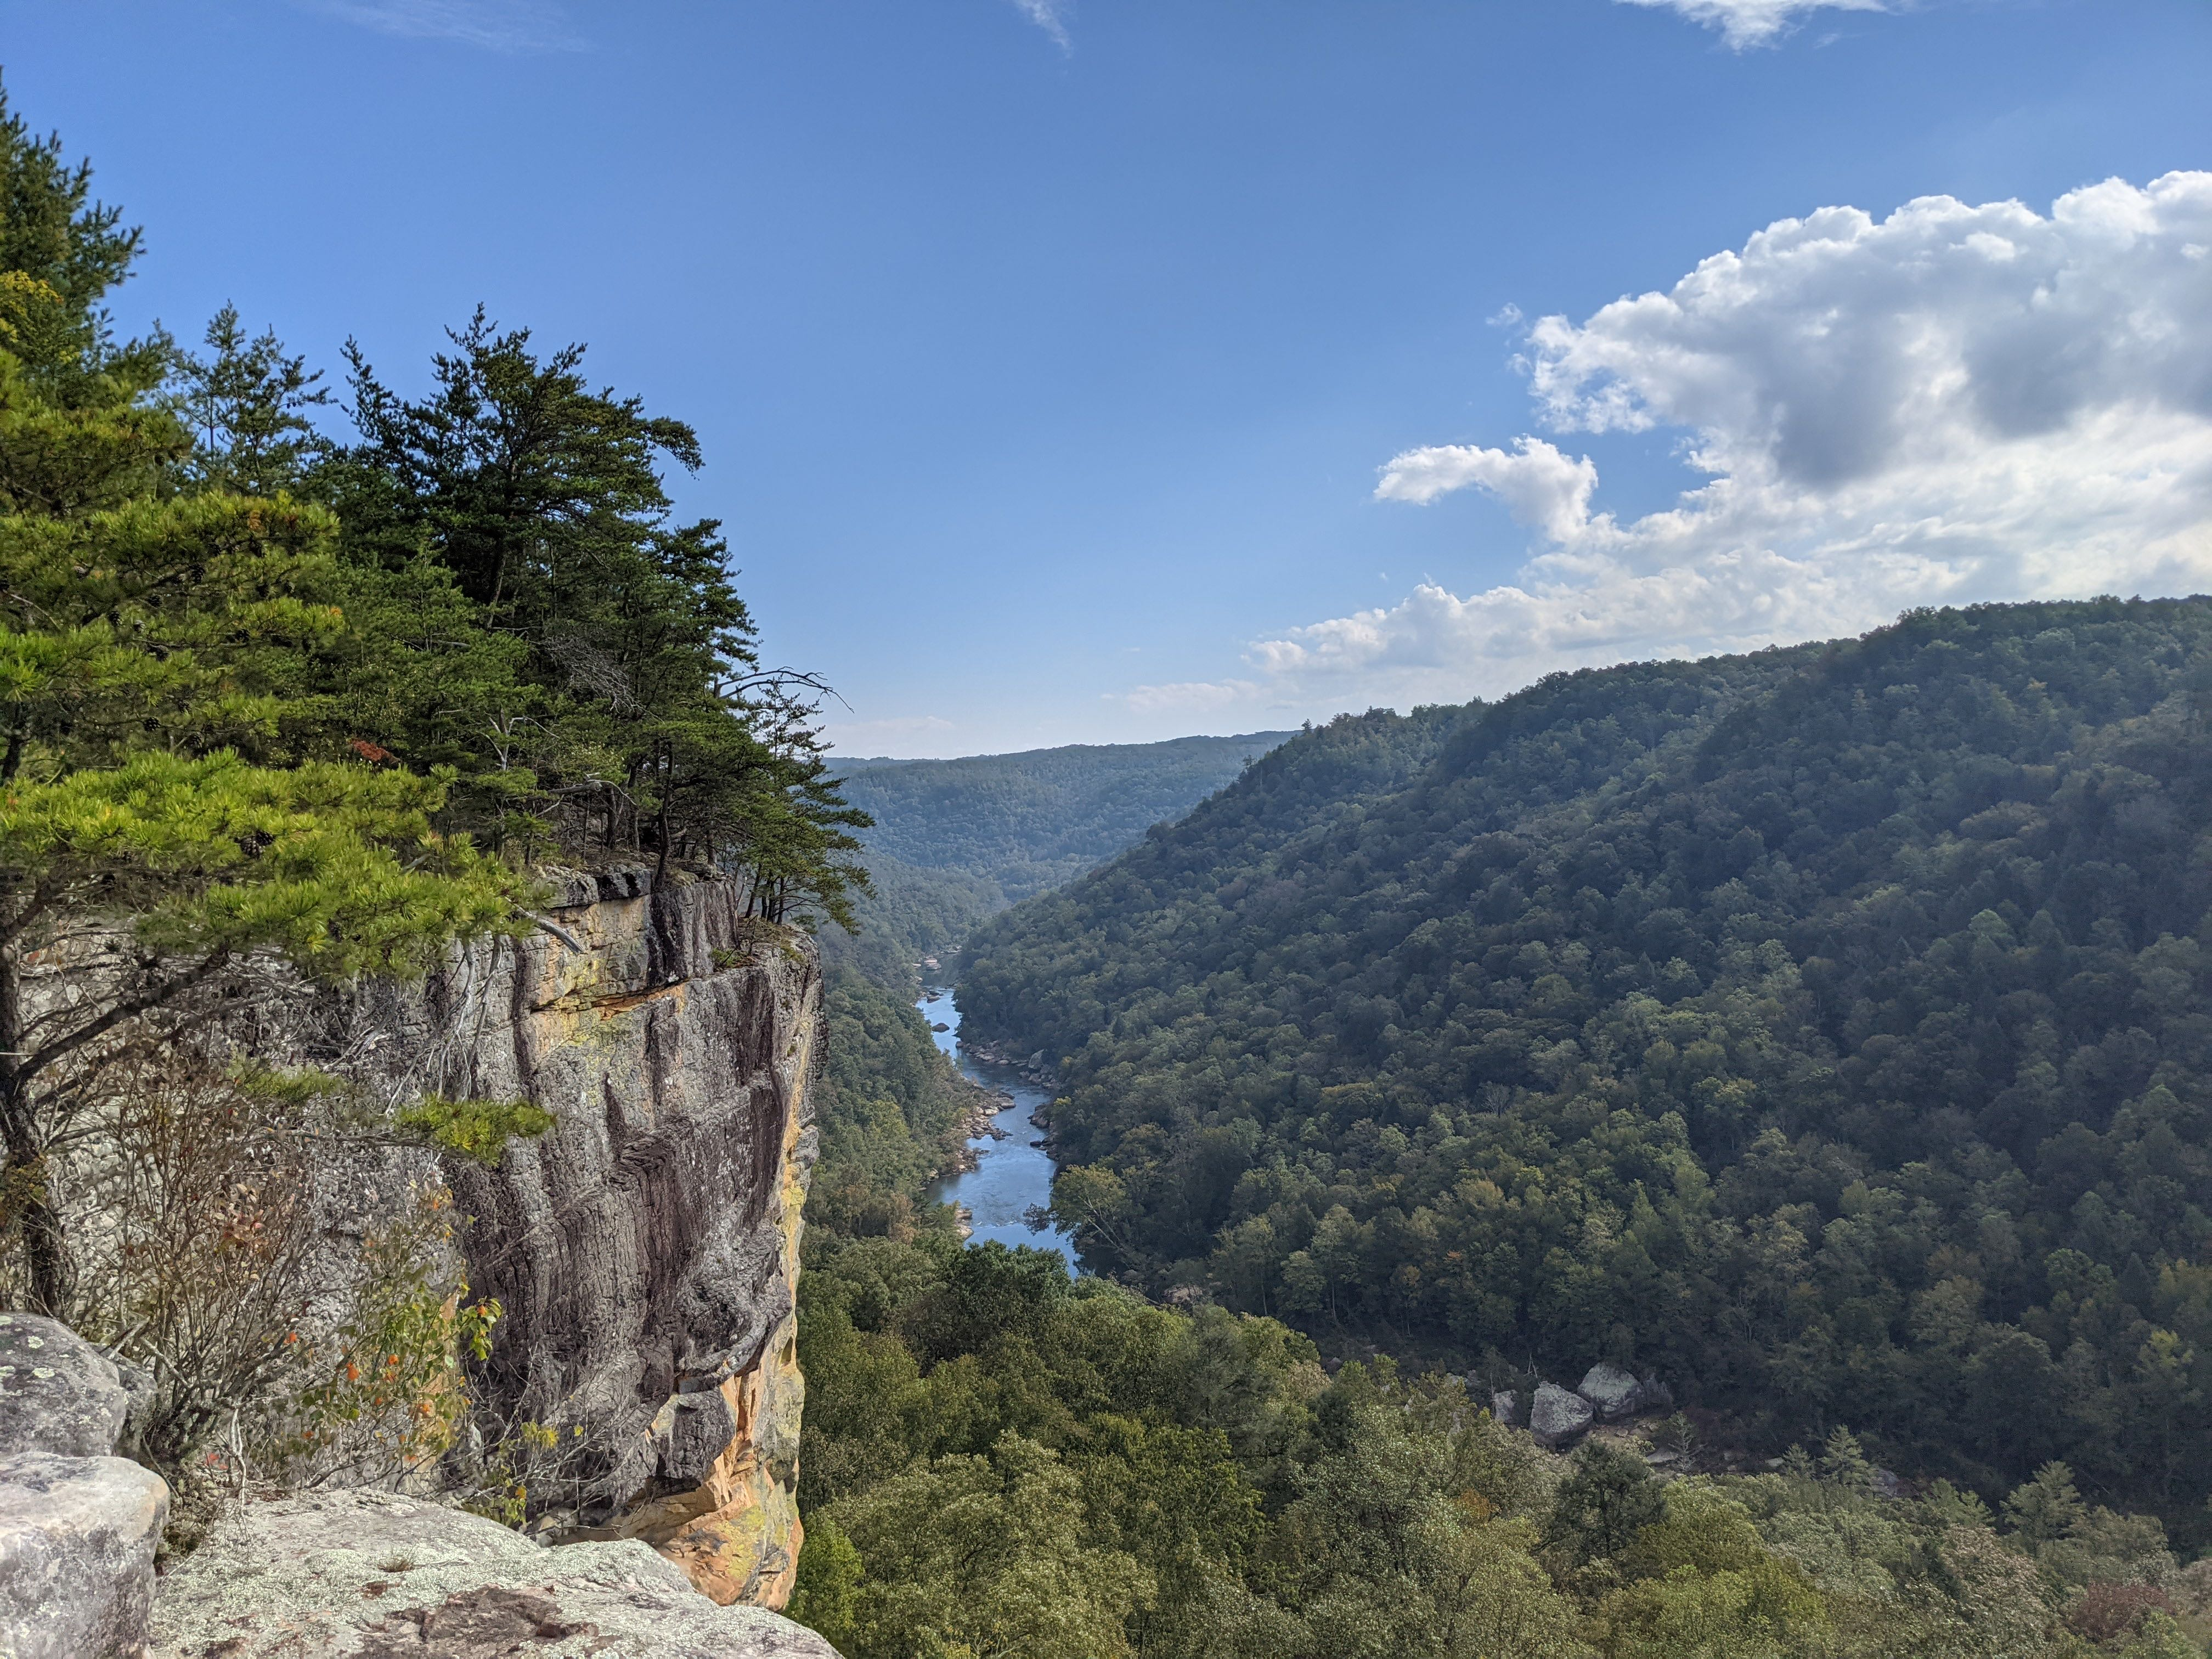
\includegraphics{img/trail-18-figure-01.jpg}

\hypertarget{directions-to-the-trailhead-17}{%
\subsubsection{Directions to the
Trailhead}\label{directions-to-the-trailhead-17}}

\begin{longtable}[]{@{}
  >{\raggedright\arraybackslash}p{(\columnwidth - 2\tabcolsep) * \real{0.5000}}
  >{\raggedright\arraybackslash}p{(\columnwidth - 2\tabcolsep) * \real{0.5000}}@{}}
\toprule\noalign{}
\begin{minipage}[b]{\linewidth}\raggedright
Trailhead Address
\end{minipage} & \begin{minipage}[b]{\linewidth}\raggedright
Grand Gap Loop Trailhead, G84V+69 Oneida, Tennessee
\end{minipage} \\
\midrule\noalign{}
\endhead
\bottomrule\noalign{}
\endlastfoot
Trailhead GPS Coordinates & 36.50549, -84.65664 \\
\end{longtable}

This address is for the trailhead for the Grand Gap Loop, deep into the
Big South Fork National River \& Recreation Area. The address uses a
Google Maps ``Plus code,'' as there is not a street address for the
trailhead. Please note this only works for Google Maps. Turn right into
the parking area from Alfred Smith Rd. Look for the Grand Gap Loop Trail
to begin the hike.

\hypertarget{trail-description-17}{%
\subsubsection{Trail Description}\label{trail-description-17}}

\begin{longtable}[]{@{}
  >{\raggedright\arraybackslash}p{(\columnwidth - 2\tabcolsep) * \real{0.5000}}
  >{\raggedright\arraybackslash}p{(\columnwidth - 2\tabcolsep) * \real{0.5000}}@{}}
\toprule\noalign{}
\begin{minipage}[b]{\linewidth}\raggedright
Distance from Start
\end{minipage} & \begin{minipage}[b]{\linewidth}\raggedright
Description
\end{minipage} \\
\midrule\noalign{}
\endhead
\bottomrule\noalign{}
\endlastfoot
0.0 & Start on the Grand Gap Loop (part of the John Muir Trail - they
share a name at this point). Head counterclockwise on the loop trail;
the other direction is a much longer way to the overlook. \\
0.85 & Grave site. \\
1.0 & Descend gently toward the overlook. \\
1.4 & Overlook. Rest and picnic at the large rocky overlook atop the Big
South Fork and Angel Falls. Then, turn around to return to the start. \\
2.8 & Trailhead. \\
\end{longtable}

\hypertarget{nearby-17}{%
\subsubsection{Nearby}\label{nearby-17}}

\begin{itemize}
\tightlist
\item
  Stopping by Bandy Creek. Check out the Bandy Creek chapter for more
  details.
\item
  Hiking the Angel Falls Trail---and others. The Angel Falls Trail---not
  to be mistaken with the trail taken to the overlook featured in this
  hike---starts at the parking area beside the Leatherwood Ford Bridge.
  It follows the Big South Fork River to conclude with a
  different---closer---view of Angel Falls, but without the vista from
  the overlook. Also, the Big South Fork National River and Recreation
  Area has more than 300 miles of trails.
\end{itemize}

\hypertarget{trail-19-honey-creek}{%
\subsection{Trail 19 : Honey Creek}\label{trail-19-honey-creek}}

\hypertarget{key-characteristics-18}{%
\subsubsection{Key Characteristics}\label{key-characteristics-18}}

\begin{longtable}[]{@{}
  >{\raggedright\arraybackslash}p{(\columnwidth - 2\tabcolsep) * \real{0.3750}}
  >{\raggedright\arraybackslash}p{(\columnwidth - 2\tabcolsep) * \real{0.6250}}@{}}
\toprule\noalign{}
\begin{minipage}[b]{\linewidth}\raggedright
Trail Name
\end{minipage} & \begin{minipage}[b]{\linewidth}\raggedright
Honey Creek Loop
\end{minipage} \\
\midrule\noalign{}
\endhead
\bottomrule\noalign{}
\endlastfoot
Region & Cumberland Plateau \\
Trail \# & 18 \\
Time Estimate - Hiking Fast & 4 hours \\
Time Estimate - Hiking Slowly & 7 hours \\
Trail Distance (Miles) & 4.4 \\
Elevation Change & Steep \\
Pets & Not Allowed \\
Parking Pass/Entrance Fee & Required \\
Restroom(s) & No \\
Terrain & Rocky path; dirt path; ladders; river rock hopping \\
\end{longtable}

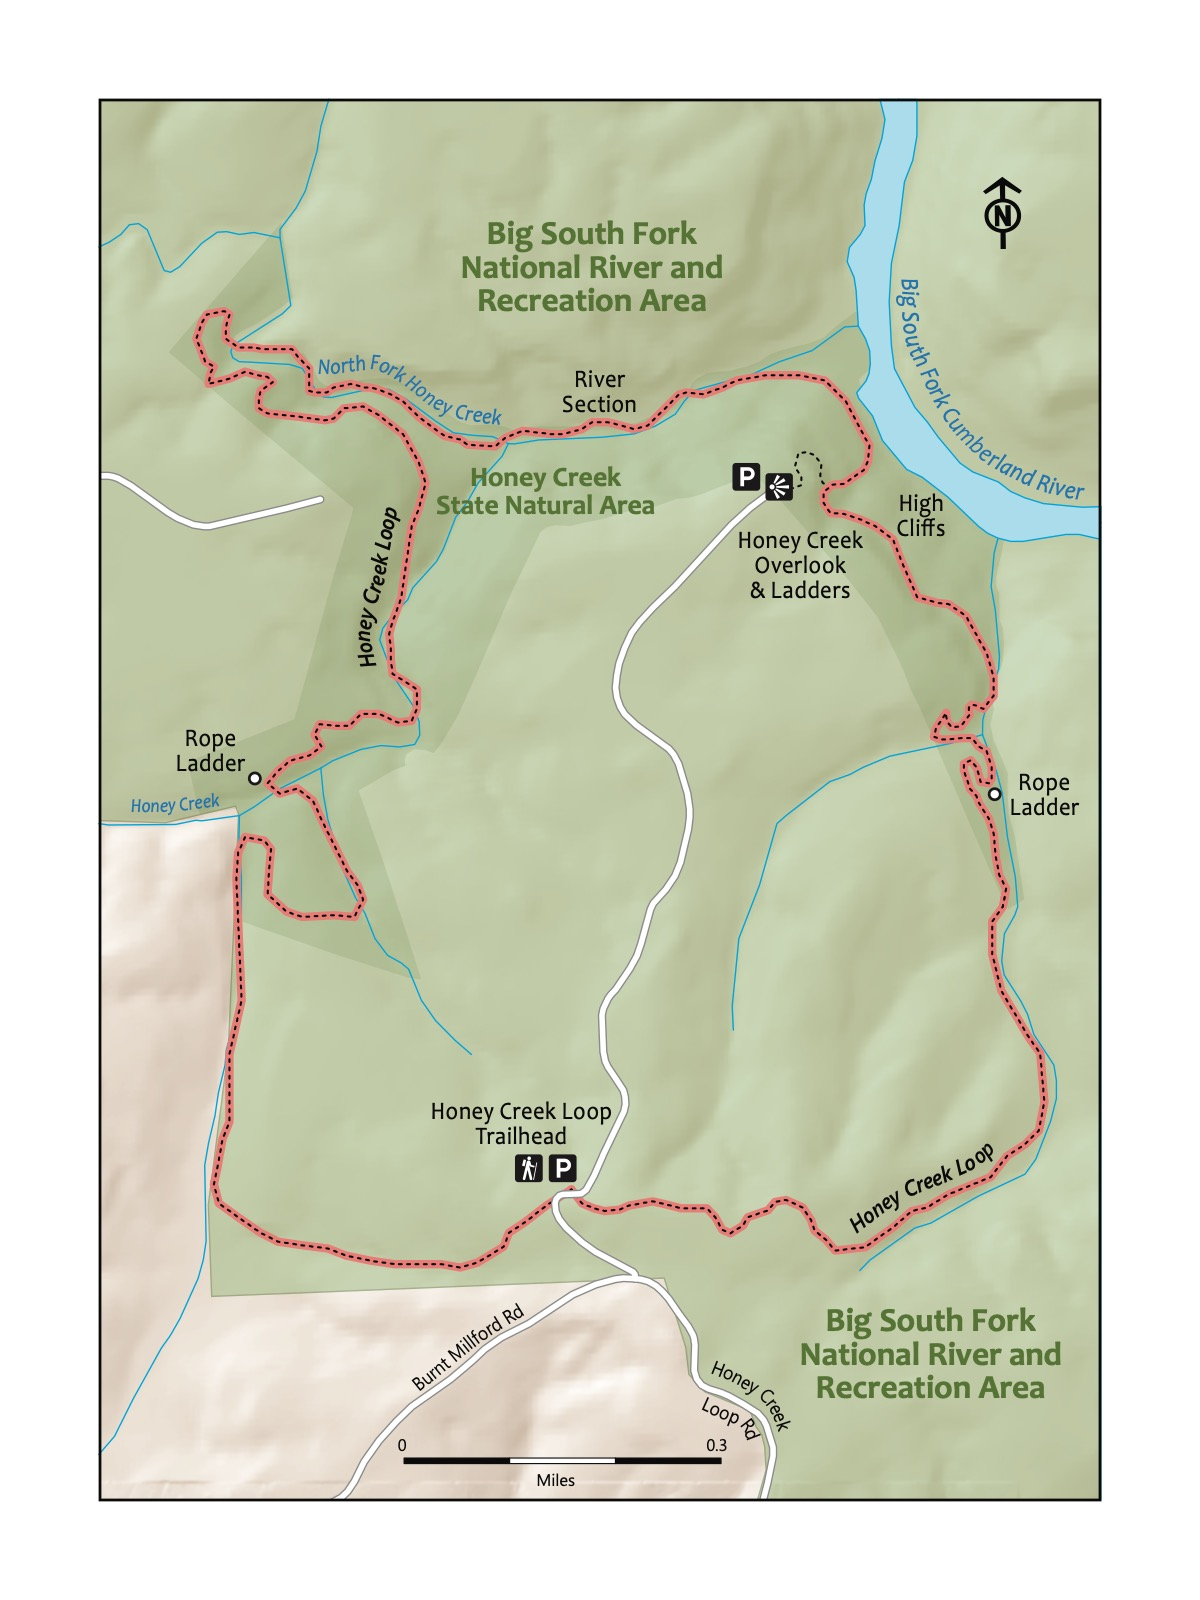
\includegraphics{maps/trail-19-map.jpeg}

\hypertarget{overview-18}{%
\subsubsection{Overview}\label{overview-18}}

Unreal! This trail features rope ladders, wooden ladders, gigantic
sandstone walls, a scenic overlook, a trail that traverses \emph{up} a
river, and boulders you crawl over and through. It's spectacular and
challenging. A memorable trail that exemplifies what makes the
Cumberland Plateau region such a worthy complement to the Great Smoky
Mountains National Park. Younger children may be able to hike the first
half (traveling counterclockwise from the trailhead); you can walk the
road back to the trailhead. The second half of the trail contains more
challenging (but very beautiful) sections. Still, it's hard --- probably
the most difficult for most in this book.

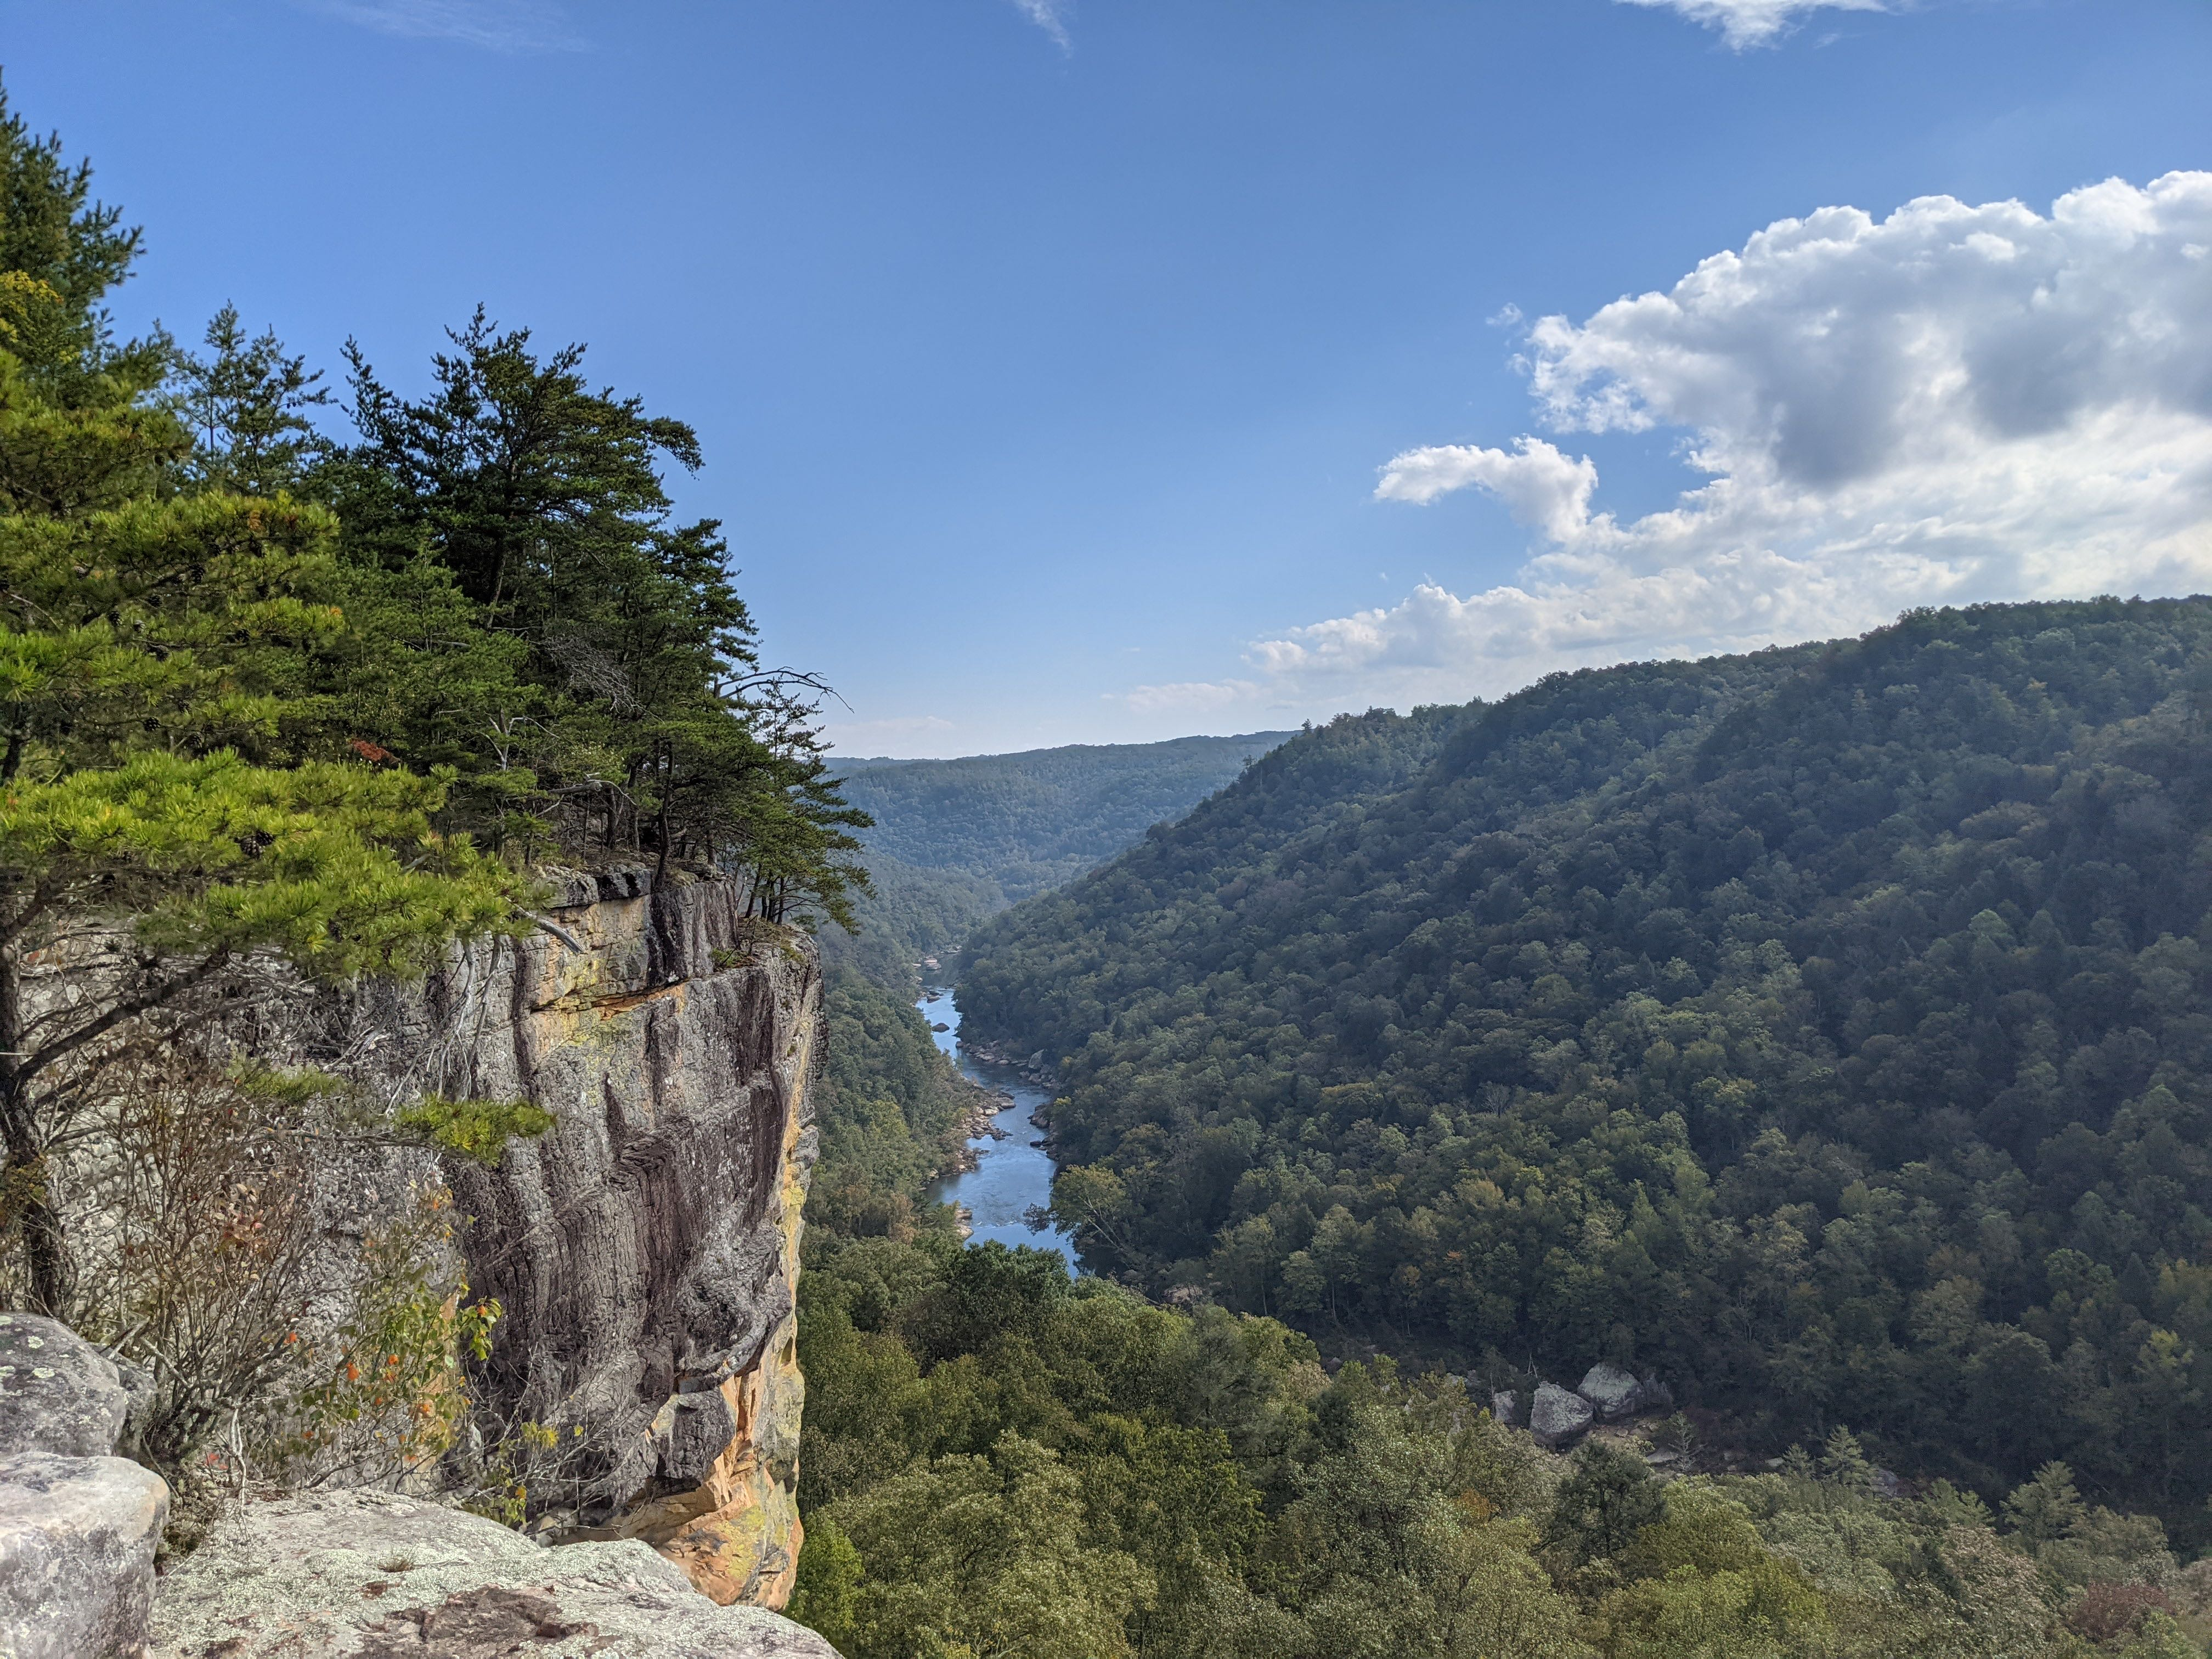
\includegraphics{img/trail-18-figure-01.jpg}

\hypertarget{directions-to-the-trailhead-18}{%
\subsubsection{Directions to the
Trailhead}\label{directions-to-the-trailhead-18}}

\begin{longtable}[]{@{}
  >{\raggedright\arraybackslash}p{(\columnwidth - 2\tabcolsep) * \real{0.5000}}
  >{\raggedright\arraybackslash}p{(\columnwidth - 2\tabcolsep) * \real{0.5000}}@{}}
\toprule\noalign{}
\begin{minipage}[b]{\linewidth}\raggedright
Trailhead Address
\end{minipage} & \begin{minipage}[b]{\linewidth}\raggedright
Honey Creek Trailhead and Parking Area, C8CX+G7 Allardt, Tennessee
\end{minipage} \\
\midrule\noalign{}
\endhead
\bottomrule\noalign{}
\endlastfoot
Trailhead GPS Coordinates & 36.42123, -84.65180 \\
\end{longtable}

Navigate to the Honey Creek Trailhead. Note that there is also a Honey
Creek Overlook --- the incorrect start for this hike. The above address
uses a Google Maps ``Plus'' code in lieu of a street address for this
trailhead; it only works in Google Maps.

Park in one of the many spots at the trailhead. The trail begins
slightly past the trailhead, on the other side of the road from the
large signpost for the trailhead, slightly up the road. Look for the
Honey Creek Loop Trail sign.

\hypertarget{trail-description-18}{%
\subsubsection{Trail Description}\label{trail-description-18}}

\begin{longtable}[]{@{}
  >{\raggedright\arraybackslash}p{(\columnwidth - 2\tabcolsep) * \real{0.5000}}
  >{\raggedright\arraybackslash}p{(\columnwidth - 2\tabcolsep) * \real{0.5000}}@{}}
\toprule\noalign{}
\begin{minipage}[b]{\linewidth}\raggedright
Distance from Start
\end{minipage} & \begin{minipage}[b]{\linewidth}\raggedright
Description
\end{minipage} \\
\midrule\noalign{}
\endhead
\bottomrule\noalign{}
\endlastfoot
0.0 & Start on the Honey Creek Loop Trail. Gently wind through the
densely wooded forest. \\
0.2 & Gently, then more steeply, descend through the woods. \\
0.9 & Rope ladder. \\
1.05 & Enter the section with high cliff walls along the left of the
trail. \\
1.35 & Trail splits to the left to head to the overlook. Ladders. \\
1.45 & Overlook. After stopping at the overlook, head back down to
resume the trail---or, optionally, walk the road back 0.8 miles to the
parking area and trailhead!). Turn left at the trail juncture to head
down toward the Big South Fork. \\
1.75 & Trail turns up into Honey Creek. This is the wildest (and most
fun) section of the trail. Look for the green symbol with two hikers as
a guide to follow the trail; in places, you'll walk on the of and even
through the creek and through crevices and cracks in giant boulders! \\
2.25 & Head up and away from the creek. \\
2.75 & Wind through and around huge boulders and rocks. Continue to look
for the green trail symbols---you're almost out of the chaotic
section! \\
3.0 & Ice Castle Falls, a beautiful waterfall. \\
3.1 & Gentle climb through a rocky, exposed section with different
vegetation. \\
3.25 & Short rope ladder. \\
3.3 & Trail levels out, then climbs back to the start and the
trailhead. \\
4.4 & Trailhead. \\
\end{longtable}

\hypertarget{nearby-18}{%
\subsubsection{Nearby}\label{nearby-18}}

\begin{itemize}
\tightlist
\item
  Grabbing a slushie! This is one of the most remote---if not the most
  remote---hikes in this book. A favorite stop on the way back from
  Honey Creek is a slushie at the Pilot Travel Center (106 Comfort Ln,
  Pioneer, TN 37847) off exit 122 on I-75.
\end{itemize}

The Great Smoky Mountains National Park is the most visited National
Park in the United States, recently an astonishing 14 million visitors
per year. It's an astonishing place --- high mountain ridges with plants
reminiscent of the northern United States and even Canada; river and
creek beds with abundant aquatic wildlife; a place of wild bears and
stories and the history of both Cherokee and European settlers still
present. There's no way around these hikes being the heart of this book.
That is not meant to diminish those close to Knoxille and the Cumberland
Plateau, which in other parts of the country would stand apart as
destinations in their own right. It just speaks to how special the
Smokies can be.

That said, a note and a warning. Many hikes in the Smokies that are
featured in this book are an hour --- some a little more, and others a
little less --- from Knoxville. The high number of visitors and the
proximity of Knoxville have key implications for families: you can be
choosy about when and where to go! While there are few things more
special than a Smokies hike up, for example, a beautiful creek on a
perfect Fall day, there are few things more challenging than being stuck
in traffic, no trail in sight, with tired out kid, or ending up on a
trail that feels more like a line at nearby Dollywood than a hike in the
woods. But, this is the benefit of living in Knoxville, and even in the
height of the summer, there are trails to visit---and times to
visit---that will surprise you with how few people there are! So, both
our trails and recommendations about them emphasize not the best trails
in general, but those that are best suited for family hikes.

\hypertarget{trail-20-spruce-flats-falls}{%
\subsection{Trail 20: Spruce Flats
Falls}\label{trail-20-spruce-flats-falls}}

\hypertarget{key-characteristics-19}{%
\subsubsection{Key Characteristics}\label{key-characteristics-19}}

\begin{longtable}[]{@{}ll@{}}
\toprule\noalign{}
Trail Name & Spruce Flats Falls \\
\midrule\noalign{}
\endhead
\bottomrule\noalign{}
\endlastfoot
Region & Great Smoky Mountains National Park \\
Trail \# & 20 \\
Time Estimate - Hiking Fast & 1.5 hours \\
Time Estimate - Hiking Slowly & 2.5 hours \\
Trail Distance (Miles) & 1.6 \\
Elevation Change & Moderate \\
Pets & Not Allowed \\
Parking Pass/Entrance Fee & Required \\
Restroom(s) & Yes \\
Terrain & Dirt path; rocky path \\
\end{longtable}

\includegraphics{maps/trail-20-map.jpeg}

\hypertarget{overview-19}{%
\subsubsection{Overview}\label{overview-19}}

An adventurous hike in the Smokies accessible to many families, it is
also a great introduction to the Smokies, particularly when visiting
from around Knoxville (it's fairly close). It's on the Great Smoky
Mountains Institute site at Tremont, a national leader in outdoors and
environmental education. It is the first hike in this section for a good
reason. The proximity to Townsend is a bonus. Best for little kids and
big kids.

\includegraphics{img/trail-20-figure-01.jpg}

\hypertarget{directions-to-the-trailhead-19}{%
\subsubsection{Directions to the
Trailhead}\label{directions-to-the-trailhead-19}}

\begin{longtable}[]{@{}ll@{}}
\toprule\noalign{}
Trailhead Address & 9275 Tremont Rd, Townsend, TN 37882 \\
\midrule\noalign{}
\endhead
\bottomrule\noalign{}
\endlastfoot
Trailhead GPS Coordinates & 35.64000, -83.68905 \\
\end{longtable}

The address and coordinates are for the Great Smoky Mountains Institute,
as this is the easiest-to-locate destination. When nearly there (less
than a quarter of a mile from the destination), you'll cross a bridge to
enter the Institute. You'll see a lot of parking around --- and the gift
shop. Though the trailhead and Google Maps will navigate you a little
further, the parking you see here is the best place to park. From this
parking lot, walk up the road a little toward the Spruce Flats Falls
Trailhead to start the hike.

\hypertarget{trail-description-19}{%
\subsubsection{Trail Description}\label{trail-description-19}}

\begin{longtable}[]{@{}
  >{\raggedright\arraybackslash}p{(\columnwidth - 2\tabcolsep) * \real{0.5000}}
  >{\raggedright\arraybackslash}p{(\columnwidth - 2\tabcolsep) * \real{0.5000}}@{}}
\toprule\noalign{}
\begin{minipage}[b]{\linewidth}\raggedright
Distance from Start
\end{minipage} & \begin{minipage}[b]{\linewidth}\raggedright
Description
\end{minipage} \\
\midrule\noalign{}
\endhead
\bottomrule\noalign{}
\endlastfoot
0.0 & You'll see signs for Spruce Flats Falls, but you'll begin
ever-so-briefly on a different trail that connects to the trail you'll
take to the falls, Buckeye Trail. Start on the Lumber Ridge Trail. \\
0.1 & Turn right onto the Buckete Trail, the trail you'll be on all the
way to the falls (and back to this spot on the return journey). \\
0.15 & Trail levels out before a steep cluimb. \\
0.3 & Climb begins. It's a (good) challenge! \\
0.5 & High point of the hike in a piney outcropping. Good photo spot.
Begin to wind down toward the waterfall. \\
0.8 & Spruce Flat Falls. A great snack or picnic spot. After a nice
break, turn around the way you came. \\
1.6 & Trailhead. \\
\end{longtable}

\hypertarget{nearby-19}{%
\subsubsection{Nearby}\label{nearby-19}}

\begin{itemize}
\tightlist
\item
  Stopping at the Tremont store. The gift store at Tremont (the full
  name is the Great Smoky Mountains Institute at Tremont) is usually
  open Monday -- Friday from 10:00 a.m. -- 4:00 p.m.
\item
  Hiking the West Prong trail. This is a great nearby trail to a great
  picnic spot (at the site of Backcountry Site \#18--- across the road
  from the Great Smoky Mountains Institute at Tremont.
\item
  Visiting Townsend. See Chestnut Tops trail for more detail.
\end{itemize}

\hypertarget{trail-21-little-river}{%
\subsection{Trail 21: Little River}\label{trail-21-little-river}}

\hypertarget{key-characteristics-20}{%
\subsubsection{Key Characteristics}\label{key-characteristics-20}}

\begin{longtable}[]{@{}ll@{}}
\toprule\noalign{}
Trail Name & Little River Loop \\
\midrule\noalign{}
\endhead
\bottomrule\noalign{}
\endlastfoot
Region & Great Smoky Mountains National Park \\
Trail \# & 19 \\
Time Estimate - Hiking Fast & 3 hours \\
Time Estimate - Hiking Slowly & 5 hours \\
Trail Distance (Miles) & 5.5 \\
Elevation Change & Moderate \\
Pets & Not Allowed \\
Parking Pass/Entrance Fee & Required \\
Restroom(s) & No \\
Terrain & Dirt path \\
\end{longtable}

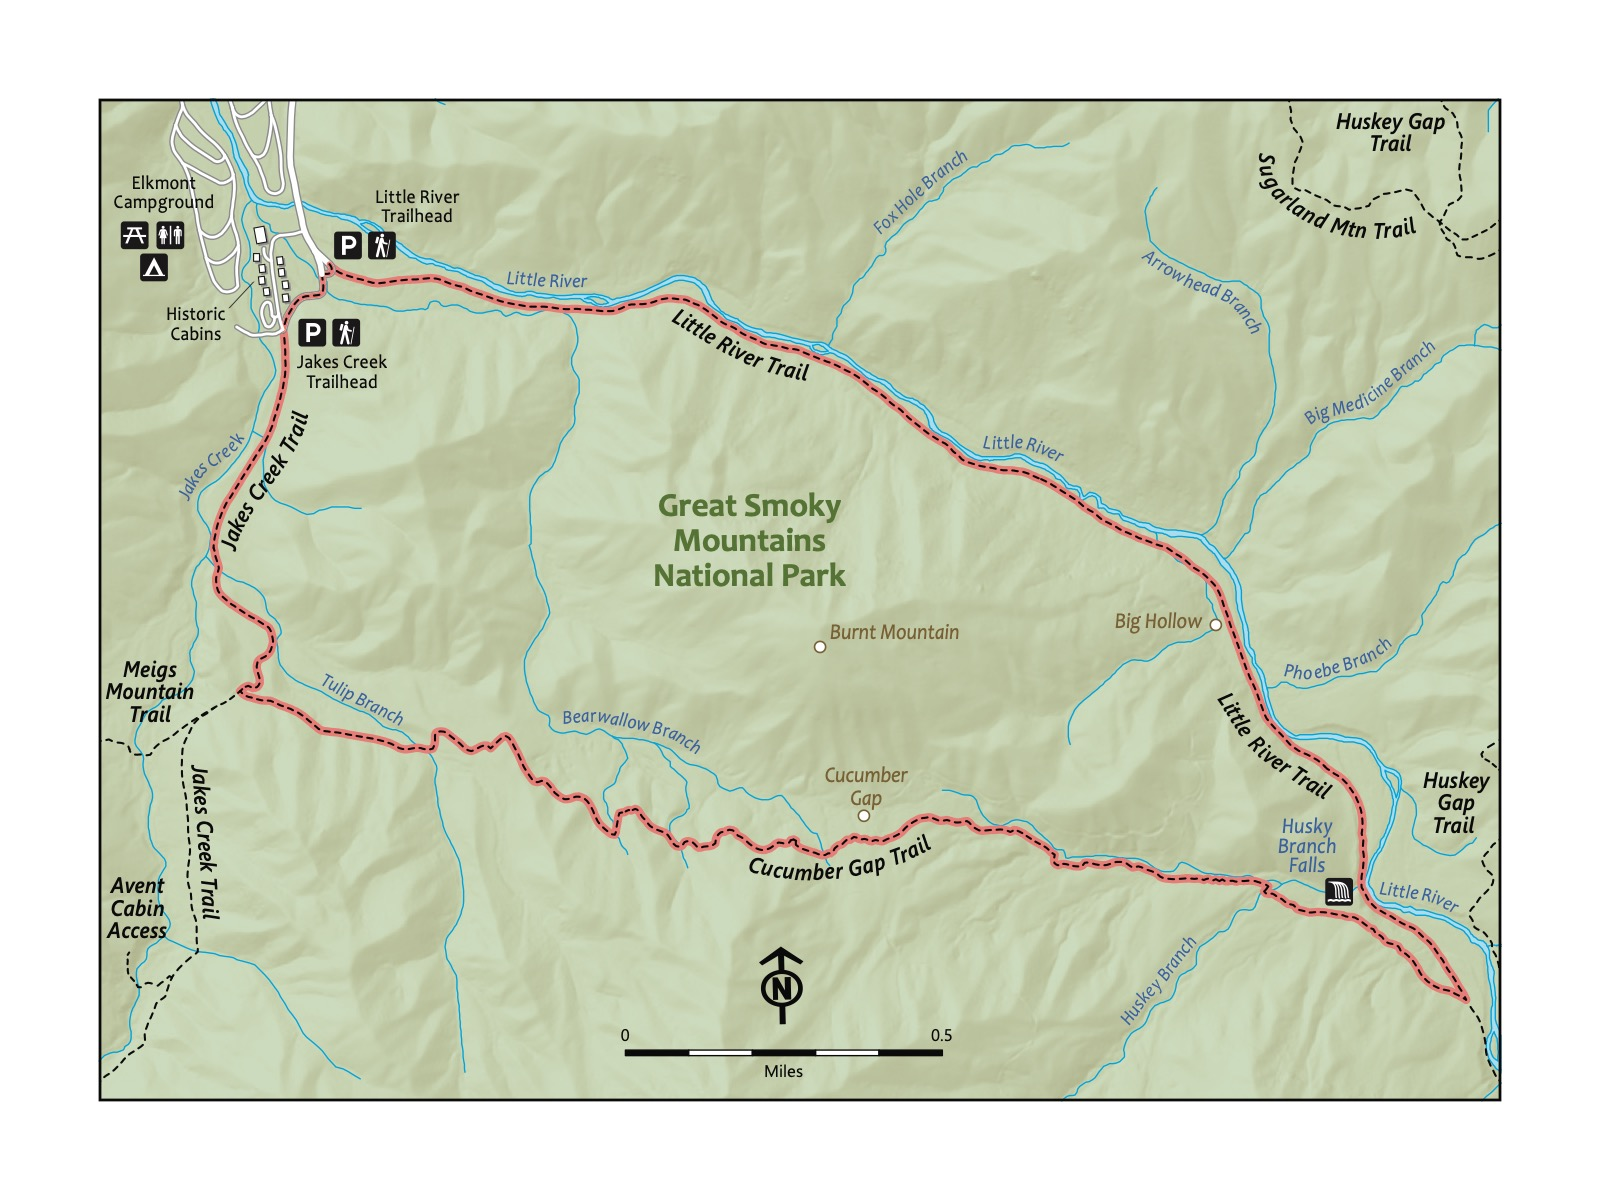
\includegraphics{maps/trail-21-map.jpeg}

\hypertarget{overview-20}{%
\subsubsection{Overview}\label{overview-20}}

This hike is a great introduction to the Great Smoky Mountains National
Park by featuring a bit of many of the elements that make the Smokies
special --- a trail along a beautiful, clear river; a waterfall;
abundant plant and aquatic wildlife; deep forest; and human history in
the form of historic cabins. It's close to many amenities, and the drive
from Knoxville is doable in a day. The hike starts at the Little River
trailhead, following the Little River along its namesake river. Turn
around near the small waterfall or continue the loop back to the
trailhead. Great for kids of all ages because there is not any one spot
you must reach on the trail; hike as far as you like and then head back
to the start to picnic or check out the historic cabins!

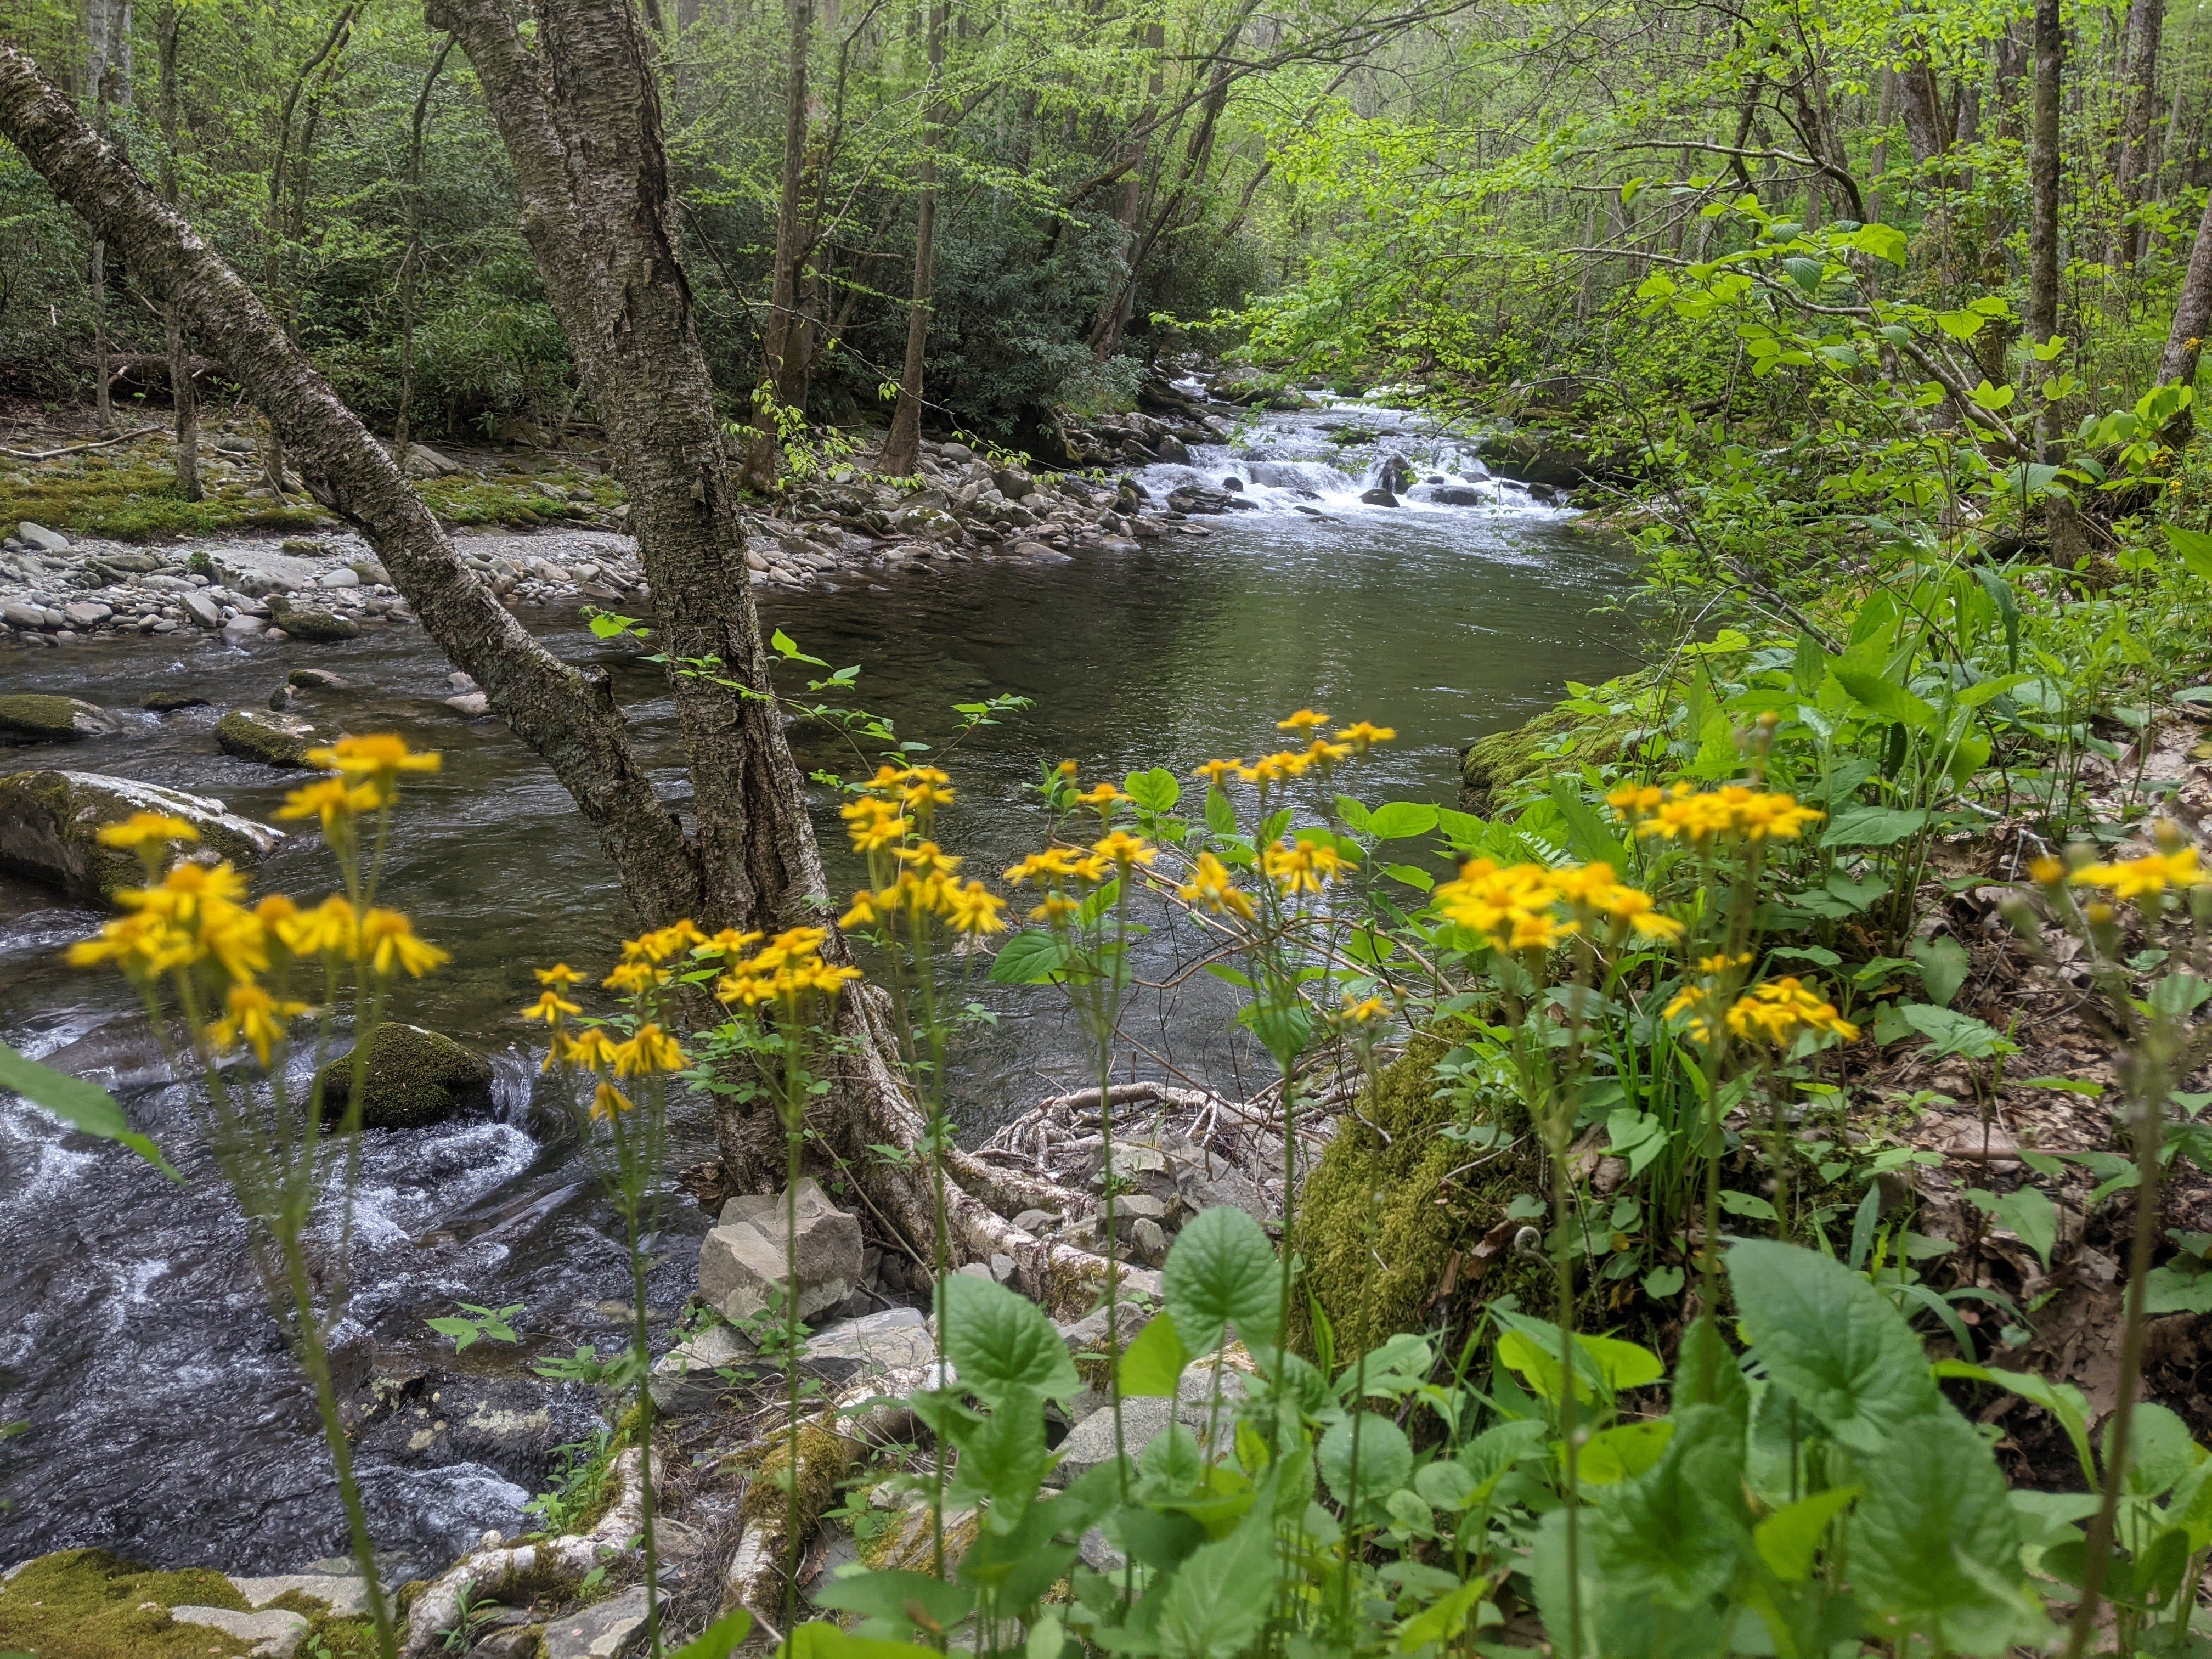
\includegraphics{img/trail-21-figure-01.jpg}

\hypertarget{directions-to-the-trailhead-20}{%
\subsubsection{Directions to the
Trailhead}\label{directions-to-the-trailhead-20}}

\begin{longtable}[]{@{}
  >{\raggedright\arraybackslash}p{(\columnwidth - 2\tabcolsep) * \real{0.5000}}
  >{\raggedright\arraybackslash}p{(\columnwidth - 2\tabcolsep) * \real{0.5000}}@{}}
\toprule\noalign{}
\begin{minipage}[b]{\linewidth}\raggedright
Trailhead Address
\end{minipage} & \begin{minipage}[b]{\linewidth}\raggedright
Elkmont Campground, MC58+3H Gatlinburg, Tennessee
\end{minipage} \\
\midrule\noalign{}
\endhead
\bottomrule\noalign{}
\endlastfoot
Trailhead GPS Coordinates & 35.65346, -83.58005 \\
\end{longtable}

The trailhead address includes a ``Plus code'' to park at the start of
the Little River Trail --- that parking area does not have a specific
address. If you navigate to ``Elkmont Campground,'' then look for signs
to the parking for the Little River Trail, where this hike begins. Park
and look for the gate across the gravel road, where the Little River
Trail begins.

\hypertarget{trail-description-20}{%
\subsubsection{Trail Description}\label{trail-description-20}}

\begin{longtable}[]{@{}
  >{\raggedright\arraybackslash}p{(\columnwidth - 2\tabcolsep) * \real{0.5000}}
  >{\raggedright\arraybackslash}p{(\columnwidth - 2\tabcolsep) * \real{0.5000}}@{}}
\toprule\noalign{}
\begin{minipage}[b]{\linewidth}\raggedright
Distance from Start
\end{minipage} & \begin{minipage}[b]{\linewidth}\raggedright
Description
\end{minipage} \\
\midrule\noalign{}
\endhead
\bottomrule\noalign{}
\endlastfoot
0.0 & Pass around the gate (it's closed only to vehicles) to begin on
the Little River Trail. \\
0.1 & Pass the Spence Cabin, a histotic cabin that is available to rent
(for the day --- not for nights!). \\
0.45 & Trail begins to ascend. \\
2.1 & Huskey Branch Falls on the right side of the trail. \\
2.4 & Reach the intersection of the Little River Trail and the Cucumber
Gap Trail. Turn right onto the Cucumber Gap trail. Trail climbs up
toward Cucumber Gap. \\
3.4 & Cucumber Gap --- the high point of this hike. Begin to descend. \\
4.65 & Reach the intersection of Cucumber Gap Trail and Jakes Creek
Trail. Turn right onto Jakes Creek Trail. \\
5.3 & Reach Jakes Creek Road. Turn right to return to the trailhead. \\
5.5 & Trailhead. \\
\end{longtable}

\includegraphics{img/trail-21-figure-02.jpg}

\hypertarget{nearby-20}{%
\subsubsection{Nearby}\label{nearby-20}}

\begin{itemize}
\tightlist
\item
  Visiting historic cabins. The nearby historic cabins are a must-see.
  Kids love to duck into and out of many recently restored (and others
  in the process of being restored).
\item
  Camping at Elkmont campground. The Elkmont Campground is scenic,
  large, and worth a visit, especially if you can reserve a spot beside
  the Little River.
\end{itemize}

\hypertarget{trail-22-mouse-creek}{%
\subsection{Trail 22: Mouse Creek}\label{trail-22-mouse-creek}}

\hypertarget{key-characteristics-21}{%
\subsubsection{Key Characteristics}\label{key-characteristics-21}}

\begin{longtable}[]{@{}ll@{}}
\toprule\noalign{}
Trail Name & Mouse Creek Falls \\
\midrule\noalign{}
\endhead
\bottomrule\noalign{}
\endlastfoot
Region & Great Smoky Mountains National Park \\
Trail \# & 20 \\
Time Estimate - Hiking Fast & 2 hours \\
Time Estimate - Hiking Slowly & 4 hours \\
Trail Distance (Miles) & 4.0 \\
Elevation Change & Moderate \\
Pets & Not Allowed \\
Parking Pass/Entrance Fee & Required \\
Restroom(s) & Yes (seasonal) \\
Terrain & Dirt path; rocky path \\
\end{longtable}

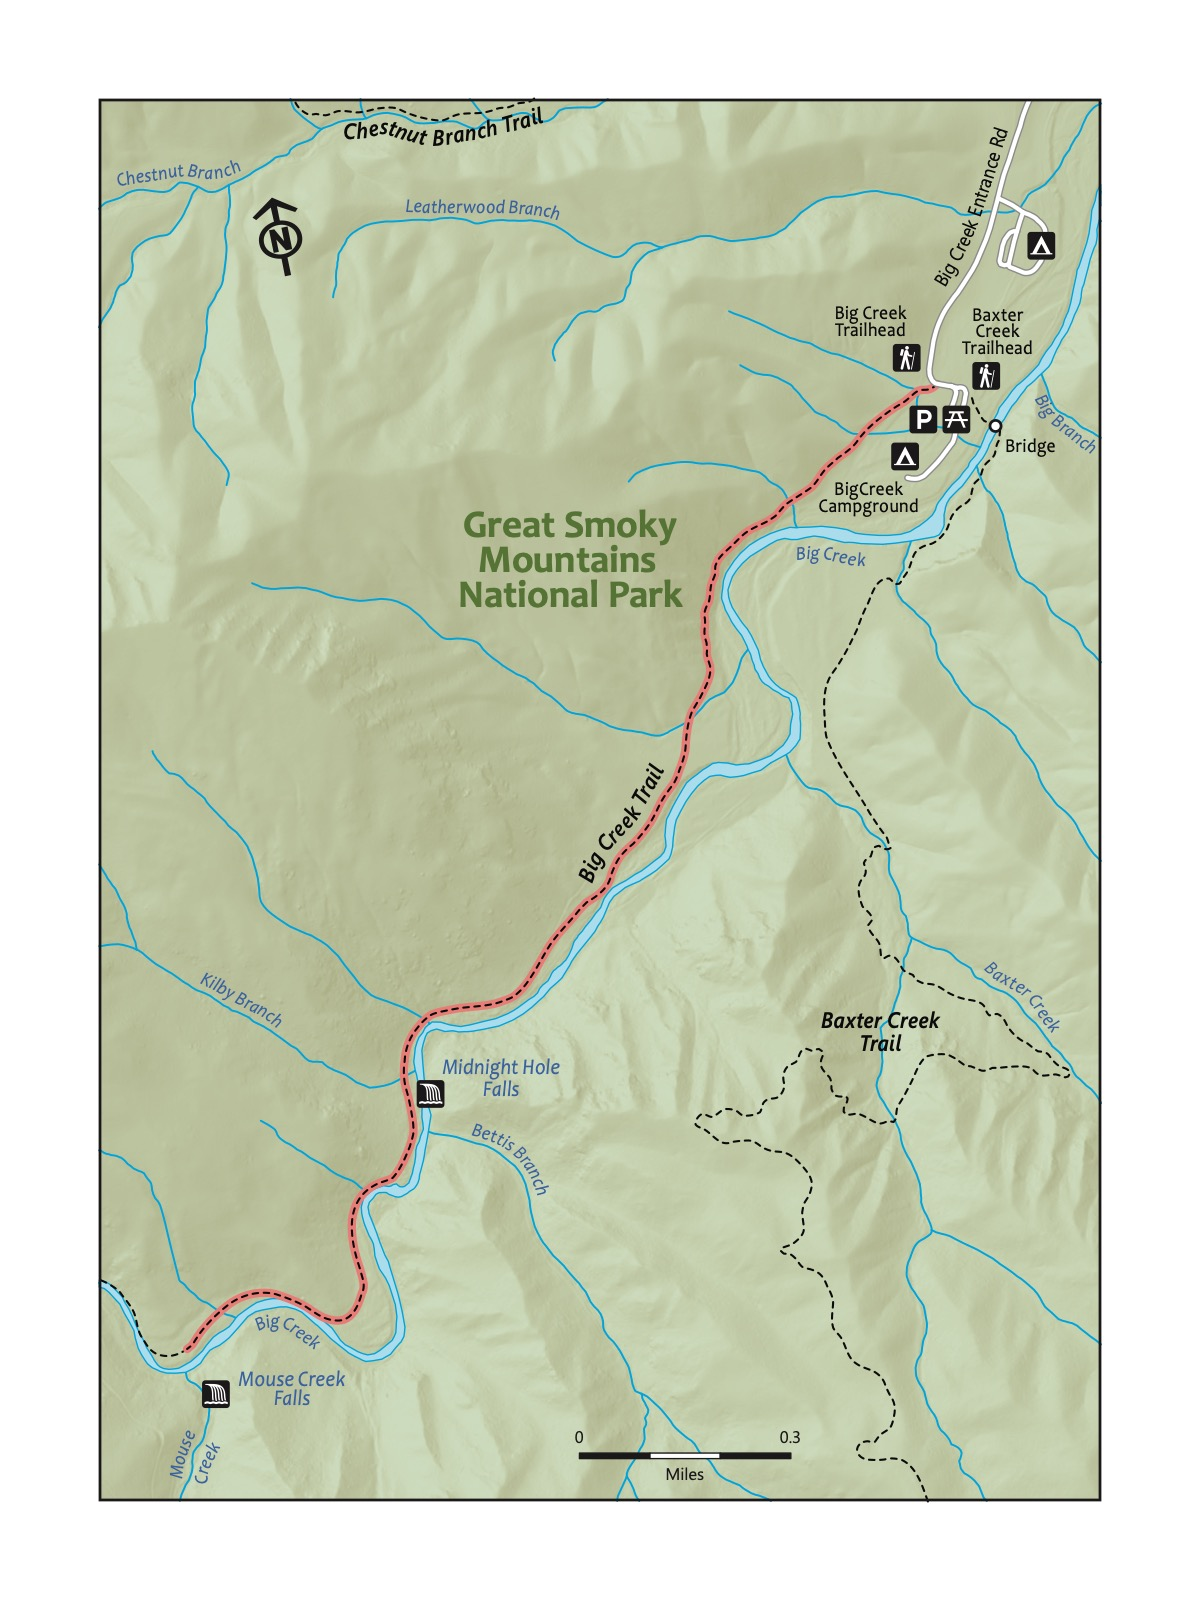
\includegraphics{maps/trail-22-map.jpeg}

\hypertarget{overview-21}{%
\subsubsection{Overview}\label{overview-21}}

Surprisingly close to Knoxville, given how remote and wild this
trailhead and trail feels, Mouse Creek in the Big Creek area of the
Smokies is quite a bit less well-known than many of the other trails in
the Great Smoky Mountains National Park in this book. The creek that
this trail follows looks otherwordly - clear and almost turquoise in
color. This hike starts at a trailhead at the Big Creek Picnic Area ---
beside the Big Creek Campground. The trail starts off a little steep,
but the trail is wide and smooth; like the Middle Prong trail, this
trail used to be a railroad bed. The trail follows above the creek and
then returns closer to it, with Mouse Creek Falls as the turn-around. A
good day-trip adventure for kids and families; the smooth grade makes
this an achievable hike for younger littles.

\includegraphics{img/trail-20-figure-01-1.jpg}

\hypertarget{directions-to-the-trailhead-21}{%
\subsubsection{Directions to the
Trailhead}\label{directions-to-the-trailhead-21}}

\begin{longtable}[]{@{}
  >{\raggedright\arraybackslash}p{(\columnwidth - 2\tabcolsep) * \real{0.5000}}
  >{\raggedright\arraybackslash}p{(\columnwidth - 2\tabcolsep) * \real{0.5000}}@{}}
\toprule\noalign{}
\begin{minipage}[b]{\linewidth}\raggedright
Trailhead Address
\end{minipage} & \begin{minipage}[b]{\linewidth}\raggedright
Big Creek Picnic Area, QV2R+H6 Newport, Tennessee
\end{minipage} \\
\midrule\noalign{}
\endhead
\bottomrule\noalign{}
\endlastfoot
Trailhead GPS Coordinates & 35.75132, -83.10964 \\
\end{longtable}

Navigate to the Big Creek Picnic Area. Note that the above address uses
a Google Maps ``Plus code'' in the absence of a street address for this
picnic area; the plus code only works in Google Maps. The picnic area is
at the end of a bumpy dirt road; it's large and easy to find. You may
note the Big Creek Trailhead on the way (it was on the right,
immediately before the parking lot). Park and then backtrack a little on
the road you took to the parking area to find the start of this trail.
Kids may like to play around the picnic area (and the pretty bridge
crossing Big Creek) before or after the hike!

\hypertarget{trail-description-21}{%
\subsubsection{Trail Description}\label{trail-description-21}}

\begin{longtable}[]{@{}
  >{\raggedright\arraybackslash}p{(\columnwidth - 2\tabcolsep) * \real{0.5000}}
  >{\raggedright\arraybackslash}p{(\columnwidth - 2\tabcolsep) * \real{0.5000}}@{}}
\toprule\noalign{}
\begin{minipage}[b]{\linewidth}\raggedright
Distance from Start
\end{minipage} & \begin{minipage}[b]{\linewidth}\raggedright
Description
\end{minipage} \\
\midrule\noalign{}
\endhead
\bottomrule\noalign{}
\endlastfoot
0.0 & Start on the Big Creek Trail. Gradually ascend. \\
0.1 & Ascend grardually on a wide path. \\
1.4 & Midnight Hole Falls. Great swimming spot in the summer. \\
2.0 & Mouse Creek Falls. Turn-around spot. Head back to the start.
Optionally, continue farther on the trail. \\
4.0 & Trailhead. \\
\end{longtable}

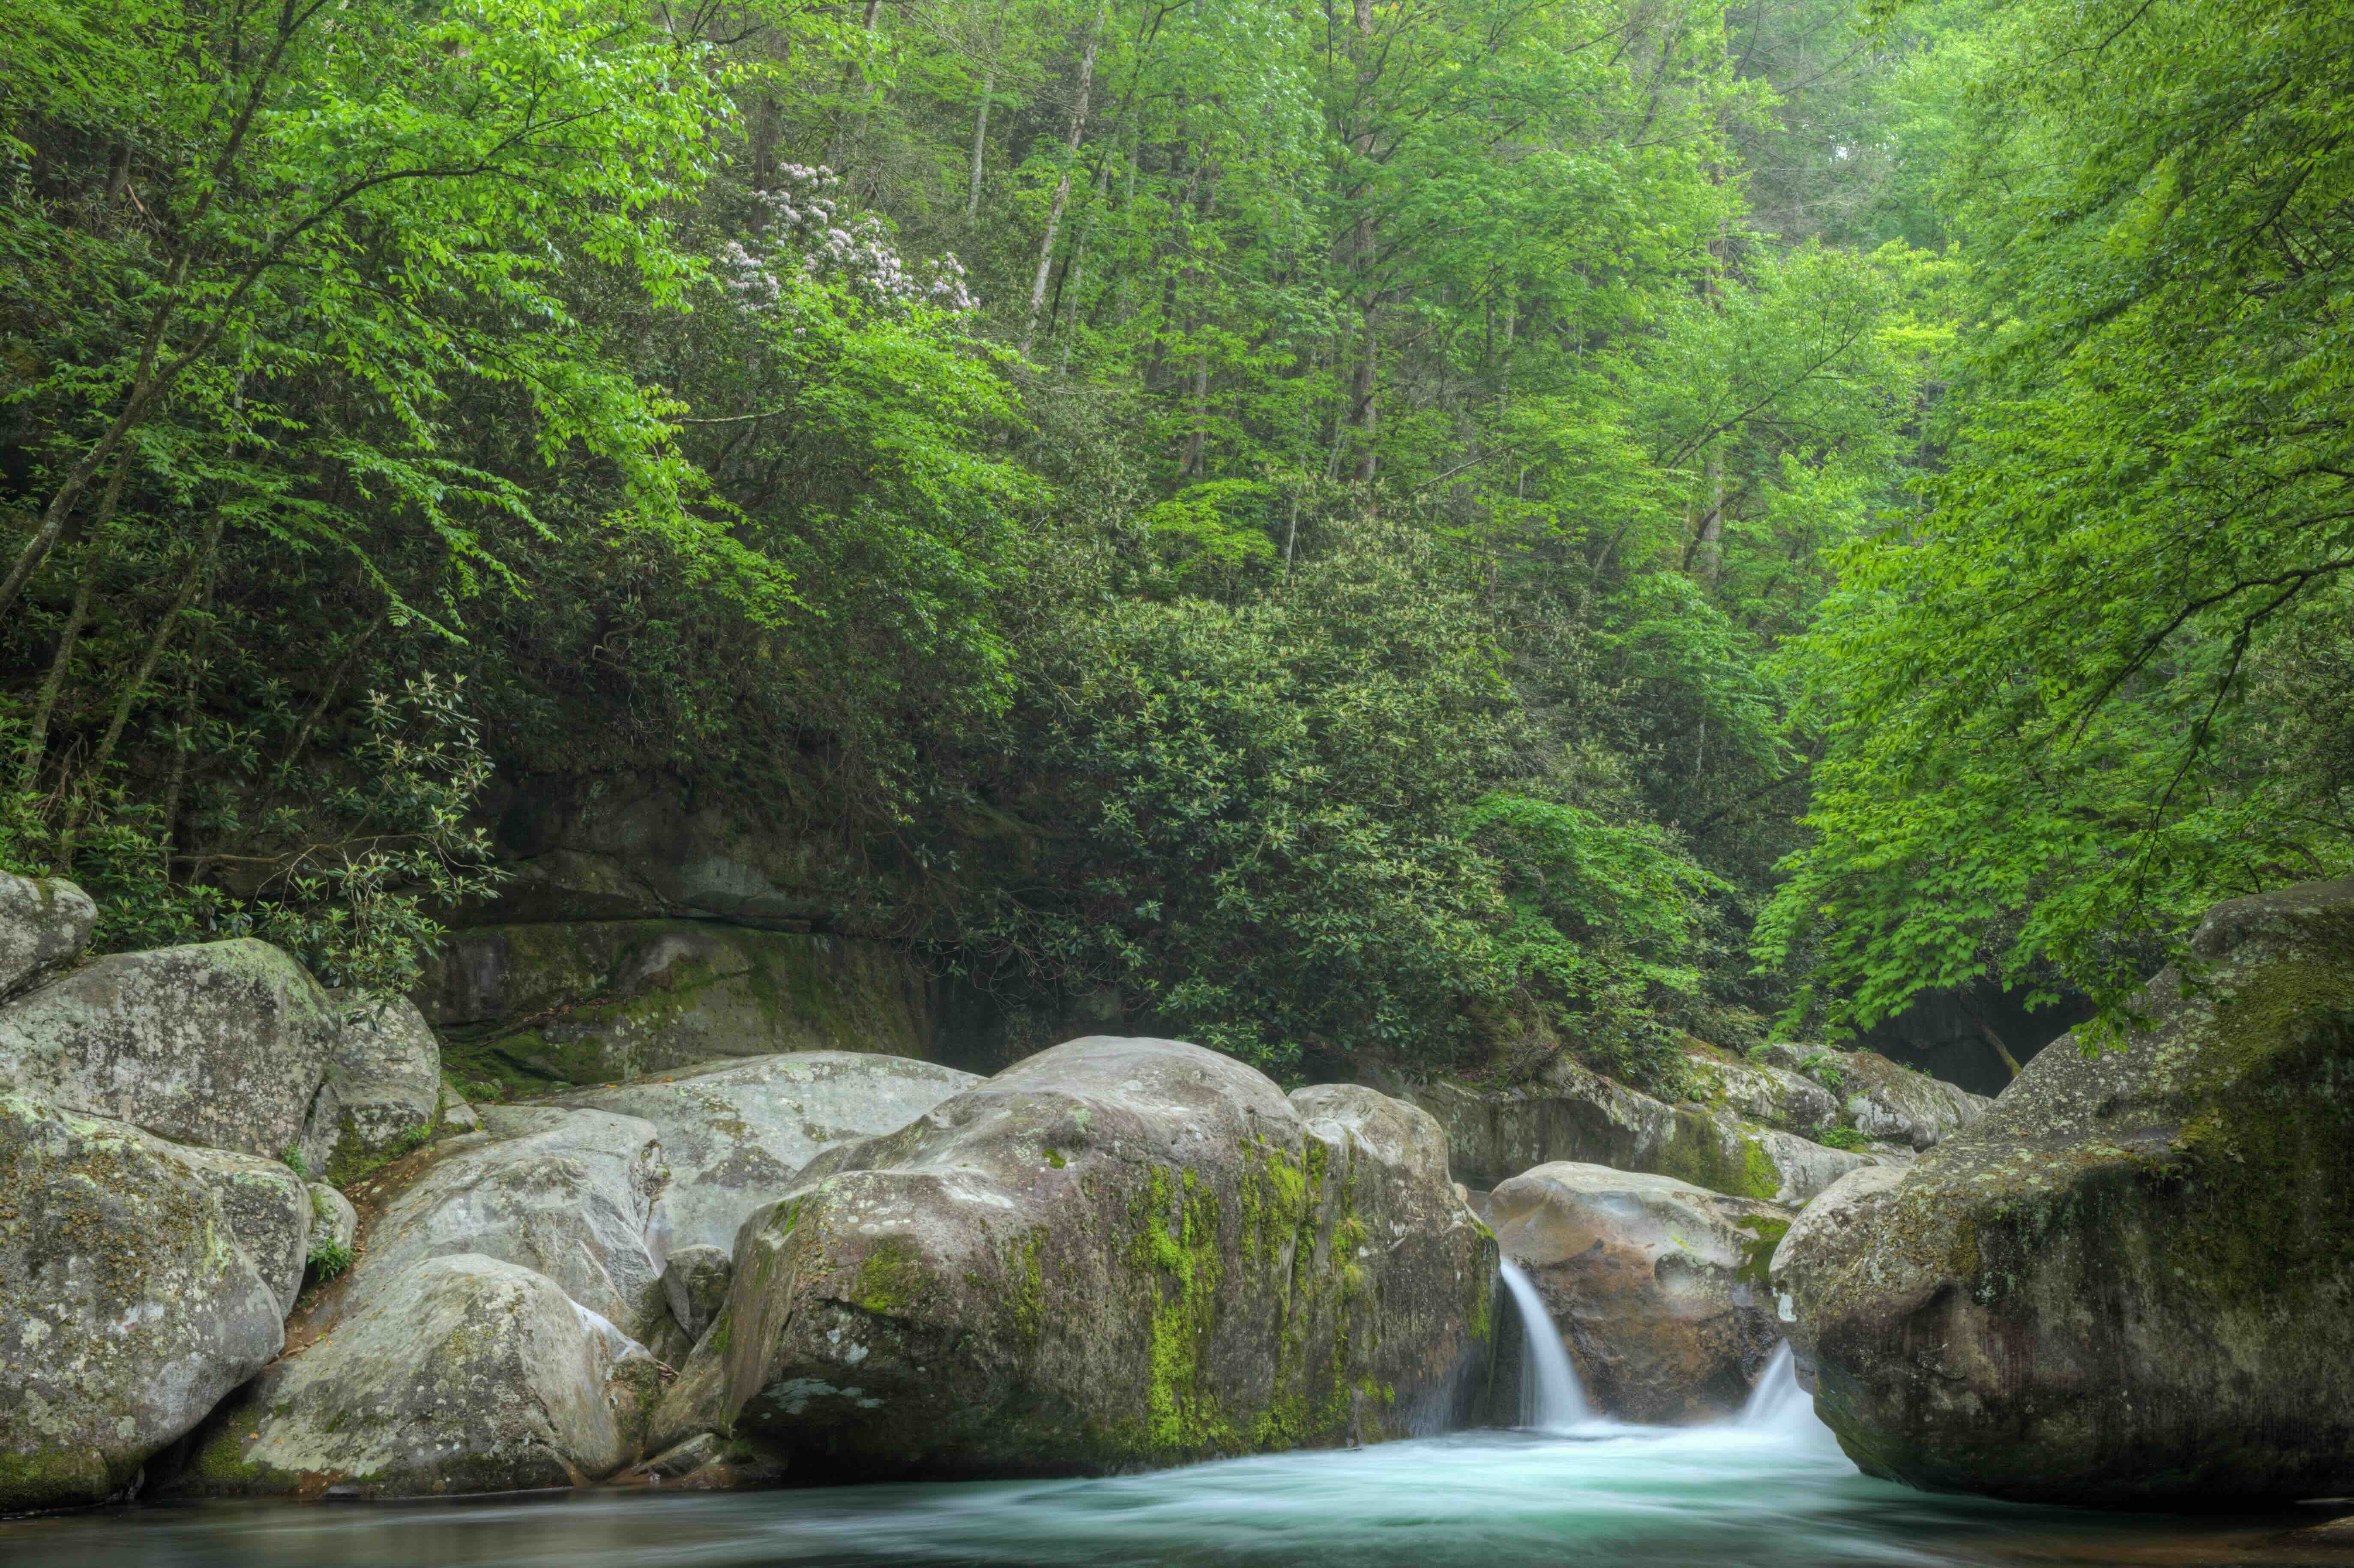
\includegraphics{img/trail-22-figure-02.jpg}

\hypertarget{nearby-21}{%
\subsubsection{Nearby}\label{nearby-21}}

\begin{itemize}
\tightlist
\item
  Picnicking at a lovely picnic area. The Big Creek Picnic Area is one
  of the finest spots to picnic in the Great Smoky Mountains National
  Park. Start or end your hike with a picnic here.
\end{itemize}

\hypertarget{trail-23-whiteoak-sink}{%
\subsection{Trail 23: Whiteoak Sink}\label{trail-23-whiteoak-sink}}

\hypertarget{key-characteristics-22}{%
\subsubsection{Key Characteristics}\label{key-characteristics-22}}

\begin{longtable}[]{@{}ll@{}}
\toprule\noalign{}
Trail Name & Whiteoak Sink \\
\midrule\noalign{}
\endhead
\bottomrule\noalign{}
\endlastfoot
Region & Great Smoky Mountains National Park \\
Trail \# & 21 \\
Time Estimate - Hiking Fast & 3 hours \\
Time Estimate - Hiking Slowly & 5 hours \\
Trail Distance (Miles) & 4.6 \\
Elevation Change & Moderate \\
Pets & Not Allowed \\
Parking Pass/Entrance Fee & Required \\
Restroom(s) & No \\
Terrain & Dirt path \\
\end{longtable}

\includegraphics{maps/trail-23-map.jpeg}

\hypertarget{overview-22}{%
\subsubsection{Overview}\label{overview-22}}

This is the wildflower hike in the Smokies. It's a joy in mid-late
April, depending on the year's weather. This hike starts on the
kid-friendly Schoolhouse Gap trail and then connects to the Whiteoak
Sink trail, which is a bit rockier but still hike-able by younger
children. You may notice that Whiteoak Sink does not appear on the
National Park Service trail map for the Smokies; technically, Whiteoak
Sink is not an official trail in the Great Smoky Mountains National
Park, and the key takeaway for hikers is to respect this unique area of
the park by staying on the trail and refraining to pick wildflowers. It
is a must-hike during wildflower season, but also worth a trip outside
of that elusive spring period. Because of the length, best for younger
kids who are carried some or all of the way, or kids who are comfortable
with a longer hike.

\includegraphics{img/trail-21-figure-01.jpg}

\hypertarget{directions-to-the-trailhead-22}{%
\subsubsection{Directions to the
Trailhead}\label{directions-to-the-trailhead-22}}

\begin{longtable}[]{@{}
  >{\raggedright\arraybackslash}p{(\columnwidth - 2\tabcolsep) * \real{0.5000}}
  >{\raggedright\arraybackslash}p{(\columnwidth - 2\tabcolsep) * \real{0.5000}}@{}}
\toprule\noalign{}
\begin{minipage}[b]{\linewidth}\raggedright
Trailhead Address
\end{minipage} & \begin{minipage}[b]{\linewidth}\raggedright
Schoolhouse Gap Trailhead, J7GF+W9, Townsend, TN 37882
\end{minipage} \\
\midrule\noalign{}
\endhead
\bottomrule\noalign{}
\endlastfoot
Trailhead GPS Coordinates & 35.62718, -83.72650 \\
\end{longtable}

The above address is for the parking area beside the trail. Please note
it uses a Google Maps ``Plus code'', as this trailhead does not have a
street address. This plus code only works in Google Maps. Park, and look
for several large boulders next to a sign for the Schoolhouse Gap Trail
to begin the hike.

\hypertarget{trail-description-22}{%
\subsubsection{Trail Description}\label{trail-description-22}}

\begin{longtable}[]{@{}
  >{\raggedright\arraybackslash}p{(\columnwidth - 2\tabcolsep) * \real{0.5000}}
  >{\raggedright\arraybackslash}p{(\columnwidth - 2\tabcolsep) * \real{0.5000}}@{}}
\toprule\noalign{}
\begin{minipage}[b]{\linewidth}\raggedright
Distance from Start
\end{minipage} & \begin{minipage}[b]{\linewidth}\raggedright
Description
\end{minipage} \\
\midrule\noalign{}
\endhead
\bottomrule\noalign{}
\endlastfoot
0.0 & Start on the Schoolhouse Gap Trail. Trail very gradually
ascends. \\
0.4 & Trail climbs more steeply (but managably!). \\
1.1 & Intersection with the trail to Whiteoak Sink. Note that Whiteoak
Sink is not an official trail on the official trail map for the Great
Smoky Mountains National Park; thus, the trail is not as well marked as
most others. Turn left from the Schoolhouse Gap trail onto the trail to
Whiteoak Sink. Descend for around .25 miles. \\
1.4 & Ascend steeply through a pretty and densely wooded forest. \\
1.7 & High point. Descend into Whiteoak Sink. \\
1.9 & Reach an intersection. The trail to the right heads to Rainbow
Cave Falls (different from and not to be confused with the Rainbow Falls
Trail near Gatlinburg!). After stopping at the waterfall, turn around to
return to the intersection of the primary trail. \\
2.2 & Turn right back onto the primary trail. Enter the part of the
trail with the densest understory of wildflowers. Tread carefully; stay
on the trail to not damage any of the plants near to the trail. \\
2.35 & Reach the large bat cave ahead of the end of the trail. Still
tread carefully (and do not attempt to enter the caves for your safety
and to not endanger the bats). Optionally, turn right or left to explore
more of this special area. Then, turn around to return along the trail
you took into Whiteoak Sink. Return to the start. \\
4.6 & Trailhead. \\
\end{longtable}

{[}{]}{[}trail-21-figure-02-1{]}

\hypertarget{nearby-22}{%
\subsubsection{Nearby}\label{nearby-22}}

\begin{itemize}
\tightlist
\item
  Exploring the Cades Cove loop. A drive around the Cades Cove Loop can
  complement a hike to Whiteoak Sink. We recommend only driving this
  beautiful loop road outside of the busiest times (summer and fall
  weekends and holidays, mainly) when traffic can be intense. Consult
  the Abrams Fall hike for additional details on this area and nearby
  amenities.
\item
  Visiting Townsend. Like the Chestnut Tops hike, visiting ``The
  Peaceful Side of the Smokies,'' Townsend, is a great way to end this
  trip to the Great Smoky Mountains National Park.
\item
  Hiking the West Prong Trail. The nearby West Prong Trail is a favorite
  that didn't quite make it into this book, but it is still a worthy
  destination. Instead of hiking up Schoolhouse Gap (like for this
  trail), cross the road and hike to the scenic backpacking site \#18 as
  the turn-around spot beside a wood log bridge and pretty creek.
\end{itemize}

\hypertarget{trail-24-middle-prong}{%
\subsection{Trail 24: Middle Prong}\label{trail-24-middle-prong}}

\hypertarget{key-characteristics-23}{%
\subsubsection{Key Characteristics}\label{key-characteristics-23}}

\begin{longtable}[]{@{}ll@{}}
\toprule\noalign{}
Trail Name & Middle Prong \\
\midrule\noalign{}
\endhead
\bottomrule\noalign{}
\endlastfoot
Region & Great Smoky Mountains National Park \\
Trail \# & 22 \\
Time Estimate - Hiking Fast & 4 hours \\
Time Estimate - Hiking Slowly & 6 hours \\
Trail Distance (Miles) & 7.6 \\
Elevation Change & Moderate \\
Pets & Not Allowed \\
Parking Pass/Entrance Fee & Required \\
Restroom(s) & No \\
Terrain & Dirt path; rocky path \\
\end{longtable}

\includegraphics{maps/trail-24-map.jpeg}

\hypertarget{overview-23}{%
\subsubsection{Overview}\label{overview-23}}

This hike is great for families looking to have an authentic hiking
experience deep in the Smokies while still being only a little over an
hour's drive from Knoxville. A benefit of this hike is its
distance--only 0.6 miles to the waterfall, but along a stream that
affords many chances to hop in and splash. The turn-around spot is an
overlook to a waterfall, Lynn Camp Prong, though the trail continues
after the cascades up to another waterfall, Indian Flats Falls. Given
the ample shade and easy access to the stream, this is a great hike for
the summer, but it is enjoyable in all seasons. Good for kids of all
ages.

\includegraphics{img/trail-24-figure-02.jpg}

\hypertarget{directions-to-the-trailhead-23}{%
\subsubsection{Directions to the
Trailhead}\label{directions-to-the-trailhead-23}}

\begin{longtable}[]{@{}
  >{\raggedright\arraybackslash}p{(\columnwidth - 2\tabcolsep) * \real{0.5000}}
  >{\raggedright\arraybackslash}p{(\columnwidth - 2\tabcolsep) * \real{0.5000}}@{}}
\toprule\noalign{}
\begin{minipage}[b]{\linewidth}\raggedright
Trailhead Address
\end{minipage} & \begin{minipage}[b]{\linewidth}\raggedright
Middle Prong Trail Trailhead, J89J+54 Townsend, Tennessee
\end{minipage} \\
\midrule\noalign{}
\endhead
\bottomrule\noalign{}
\endlastfoot
Trailhead GPS Coordinates & 35.61794, -83.66971 \\
\end{longtable}

The above address will navigate you to the parking area for the
trailhead. Please note it uses a ``Plus code'' in lieu of a stree
address that only works in Google Maps. Note that this trailhead is at
the end of a lengthy gravel road, but it's fairly smooth (and it's a
pretty drive). This is a large parking area. Even on the busiest days,
you will be able to find a place to park. There are spots around the
turn-around, but, if they are taken, it is acceptable to park on the
side of the road. After parking, walk toward the bridge to start your
hike.

\hypertarget{trail-description-23}{%
\subsubsection{Trail Description}\label{trail-description-23}}

\begin{longtable}[]{@{}
  >{\raggedright\arraybackslash}p{(\columnwidth - 2\tabcolsep) * \real{0.5000}}
  >{\raggedright\arraybackslash}p{(\columnwidth - 2\tabcolsep) * \real{0.5000}}@{}}
\toprule\noalign{}
\begin{minipage}[b]{\linewidth}\raggedright
Distance from Start
\end{minipage} & \begin{minipage}[b]{\linewidth}\raggedright
Description
\end{minipage} \\
\midrule\noalign{}
\endhead
\bottomrule\noalign{}
\endlastfoot
0.0 & Cross the bridge over Lynn Camp Prong. Ascend gradually on the
Middle Prong Trail. \\
0.05 & Almost immediately past the bridge, not the split in the trail.
This hike heads to the left. A short trail, the Thunderhead Prong Quiet
Walkway, heads to the left (it's a great place for kids to play and
splash on hot days!). \\
0.65 & Overlook to Lynn Camp Prong. Though a short way in, this is an
acceptable spot to turn around and head back to the start. The trail
continues onward. This is one of many trails in the Smokies that is
pretty and very worthwhile all along the way; hike as far as you or your
littles like. \\
2.35 & Intersection with Panther Creek Trail on the left. Continue on
the Middle Prong Trail. \\
3.6 & Begin a brief switchback before the waterfall at the end of this
hike. \\
3.8 & Reach Indian Flat Falls. Look for a little opening in the trees
and shrubs. You'll find it! After resting at the beautiful waterfall,
turn around to return to the start. \\
5.25 & Intersection with the Panther Creek Trail on the right. \\
7.6 & Trailhead \\
\end{longtable}

\includegraphics{img/trail-22-figure-01.jpg}

\hypertarget{nearby-23}{%
\subsubsection{Nearby}\label{nearby-23}}

\begin{itemize}
\tightlist
\item
  Driving the Cade's Cove Loop. This is a nice way to make a longer day
  of your trip. Instead of returning the way you came, at the
  intersection of Townsend Road and Laurel Creek Road, turn left and
  head toward Cade's Cove. The drive to Cade's Cove is around 15
  minutes; the loop road around Cade's Cove takes around 45 minutes to
  drive--longer on busy days, especially when bears are visible--which
  is often! Traffic on the loop road can be severe, especially during
  peak times, so plan accordingly to avoid restless kiddos.
\item
  Stopping for a snack or meal in Townsend. Townsend bills itself as the
  ``Peaceful Side of the Smokies''. Peaceful Side Social is a favorite
  lunch and dinner spot with kids, owing to the good food and large
  outdoor play area.
\end{itemize}

\hypertarget{trail-25-abrams-creek}{%
\subsection{Trail 25: Abrams Creek}\label{trail-25-abrams-creek}}

\hypertarget{key-characteristics-24}{%
\subsubsection{Key Characteristics}\label{key-characteristics-24}}

\begin{longtable}[]{@{}
  >{\raggedright\arraybackslash}p{(\columnwidth - 2\tabcolsep) * \real{0.4028}}
  >{\raggedright\arraybackslash}p{(\columnwidth - 2\tabcolsep) * \real{0.5972}}@{}}
\toprule\noalign{}
\begin{minipage}[b]{\linewidth}\raggedright
Trail Name
\end{minipage} & \begin{minipage}[b]{\linewidth}\raggedright
Abrams Creek
\end{minipage} \\
\midrule\noalign{}
\endhead
\bottomrule\noalign{}
\endlastfoot
Region & Great Smoky Mountains National Park \\
Trail \# & 23 \\
Time Estimate - Hiking Fast & 4 hours \\
Time Estimate - Hiking Slowly & 6 hours \\
Trail Distance (Miles) & 5.8 \\
Elevation Change & Moderate \\
Pets & Not Allowed \\
Parking Pass/Entrance Fee & Required \\
Restroom(s) & Yes (seasonal) \\
Terrain & Dirt path; rocky path; small creek crossings \\
\end{longtable}

\includegraphics{maps/trail-25-map.jpeg}

\hypertarget{overview-24}{%
\subsubsection{Overview}\label{overview-24}}

Abrams Creek is a great place to start hiking in the Smokies if you live
in or around Knoxville. It's accessible, offers a wide variety of
features to please all members of the family, and has the added bonus of
being beautiful! The enduring memory from this trail is of kids
splashing endlessly in the shallow creeks. This was the first place we
traveled as a family in the Smokies, and we returned again and again
because we always enjoyed our time together there. There are many ways
to shorten the hike, and we often hike around a mile in and then turn
around. It can be warmer here in the summer months, but the river offers
many opportunities to swim and splash around, making it a great
destination for the summer as well. This hike is relatively challenging
and better suited to hiking with older children, but the beauty of this
hike is its versatility.

\includegraphics{img/trail-23-figure-01.jpg}

\hypertarget{directions-to-the-trailhead-24}{%
\subsubsection{Directions to the
Trailhead}\label{directions-to-the-trailhead-24}}

\begin{longtable}[]{@{}
  >{\raggedright\arraybackslash}p{(\columnwidth - 2\tabcolsep) * \real{0.5000}}
  >{\raggedright\arraybackslash}p{(\columnwidth - 2\tabcolsep) * \real{0.5000}}@{}}
\toprule\noalign{}
\begin{minipage}[b]{\linewidth}\raggedright
Trailhead Address
\end{minipage} & \begin{minipage}[b]{\linewidth}\raggedright
Abrams Creek Campground, J368+MR Tallassee, Tennessee
\end{minipage} \\
\midrule\noalign{}
\endhead
\bottomrule\noalign{}
\endlastfoot
Trailhead GPS Coordinates & 35.61095, -83.93356 \\
\end{longtable}

It never seems to become crowded at Abrams Creek, but parking can be a
bit confusing. This is because the campground is further along the same
road the trailhead is on. Also, there are two areas to park for the
trailhead. We usually park by the gate to the campground, but you can
also park near the large sign with maps of this area of the national
park.

\hypertarget{trail-description-24}{%
\subsubsection{Trail Description}\label{trail-description-24}}

\begin{longtable}[]{@{}
  >{\centering\arraybackslash}p{(\columnwidth - 2\tabcolsep) * \real{0.5000}}
  >{\centering\arraybackslash}p{(\columnwidth - 2\tabcolsep) * \real{0.5000}}@{}}
\toprule\noalign{}
\begin{minipage}[b]{\linewidth}\centering
Distance from Start
\end{minipage} & \begin{minipage}[b]{\linewidth}\centering
Description
\end{minipage} \\
\midrule\noalign{}
\endhead
\bottomrule\noalign{}
\endlastfoot
0.0 & Start at the trailhead parking area. Walk along the road beside
Abrams Creek. \\
0.4 & Arrive at the campground. A great spot to rest and hang out by the
creek. \\
1.0 & Cross Kingfisher Creek for the first time. Watch for rocks and
branches to aid in crossing. \\
1.1 & Cross Kingfisher Creek again about 100 yards past the first
crossing. \\
1.3 & Reach Backcountry Site \#1. Frequently used by overnight
backpackers; a good resting spot. We often turn around here! \\
1.5 & Reach the top of the ridge after a steep climb. Another great
place to stop and rest (or turn around). Or continue for a grand
adventure. \\
1.6 & Arrive at the overlook with views of Abrams Creek and Gregory Bald
in the distance. \\
2.0 & Return to Abrams Creek near its intersection with Buckshank
Branch. A great spot to relax and splash in the creek. \\
2.8 & Reach Backcountry Site \#17. Turn around here to head back to the
start. \\
4.3 & Return to Backcountry Site \#1. \\
5.6 & Trailhead. \\
\end{longtable}

\includegraphics{img/trail-25-figure-03.jpg}

\hypertarget{nearby-24}{%
\subsubsection{Nearby}\label{nearby-24}}

\begin{itemize}
\tightlist
\item
  Visiting the Look Rock Overlook. Check the Look Rock Overlook hike for
  a short, nearby hike to a pretty overlook.
\item
  Camping at Abrams Creek Campground. This is a lovely creekside
  campground that you pass on this hike. Consider a stay in the summer,
  when jumping in the cool, not-too-deep creek can be a respite from the
  heat---or in the fall when this area pops with fall colors.
\end{itemize}

\hypertarget{trail-26-look-rock}{%
\subsection{Trail 26: Look Rock}\label{trail-26-look-rock}}

\hypertarget{key-characteristics-25}{%
\subsubsection{Key Characteristics}\label{key-characteristics-25}}

\begin{longtable}[]{@{}ll@{}}
\toprule\noalign{}
Trail Name & Look Rock Overlook \\
\midrule\noalign{}
\endhead
\bottomrule\noalign{}
\endlastfoot
Region & Great Smoky Mountains National Park \\
Trail \# & 24 \\
Time Estimate - Hiking Fast & 30 minutes \\
Time Estimate - Hiking Slowly & 1 hour \\
Trail Distance (Miles) & 0.6 \\
Elevation Change & Moderate \\
Pets & Not Allowed \\
Parking Pass/Entrance Fee & Required \\
Restroom(s) & No \\
Terrain & Paved path \\
\end{longtable}

\includegraphics{maps/trail-26-map.jpeg}

\hypertarget{overview-25}{%
\subsubsection{Overview}\label{overview-25}}

This is a short but rewarding overlook hike that is just a moderate
drive from Knoxville. The entire hike is paved --- but the trail is
steep. Start at a parking area with a very scenic overlook. The trail
starts steep but then levels out. At the top is a tower that affords
views of the Smokies as well as the Tennessee Valley and Knoxville.
Clear days are more often found in the winter, spring, and fall (after
the humidity drops). Consider coupling with a drive along the Foothills
Parkway, or take visitors here after you pick them up from the airport
in nearby Maryville, as we have with our parents! This is a fun family
thike with littles that serve as a nice and usually not crowded
introduction to the Smokies.
\includegraphics{img/trail-24-figure-01.jpg}

\hypertarget{directions-to-the-trailhead-25}{%
\subsubsection{Directions to the
Trailhead}\label{directions-to-the-trailhead-25}}

\begin{longtable}[]{@{}
  >{\raggedright\arraybackslash}p{(\columnwidth - 2\tabcolsep) * \real{0.5000}}
  >{\raggedright\arraybackslash}p{(\columnwidth - 2\tabcolsep) * \real{0.5000}}@{}}
\toprule\noalign{}
\begin{minipage}[b]{\linewidth}\raggedright
Trailhead Address
\end{minipage} & \begin{minipage}[b]{\linewidth}\raggedright
Look Rock Lower Overlook, 7210 Flats Rd, Tallassee, TN 37878
\end{minipage} \\
\midrule\noalign{}
\endhead
\bottomrule\noalign{}
\endlastfoot
Trailhead GPS Coordinates & 35.63099, -83.94083 \\
\end{longtable}

The above address takes you to a large parking lot with a scenic
overlook. Park, and look for the scenic overlook---the Murry Gap
Overlook. From there, walk along the back of the parking lot, and then
along a sidewalk. Cross the road to the Look Rock Trail to begin the
hike.

\hypertarget{trail-description-25}{%
\subsubsection{Trail Description}\label{trail-description-25}}

\begin{longtable}[]{@{}
  >{\raggedright\arraybackslash}p{(\columnwidth - 2\tabcolsep) * \real{0.5000}}
  >{\raggedright\arraybackslash}p{(\columnwidth - 2\tabcolsep) * \real{0.5000}}@{}}
\toprule\noalign{}
\begin{minipage}[b]{\linewidth}\raggedright
Distance from Start
\end{minipage} & \begin{minipage}[b]{\linewidth}\raggedright
Description
\end{minipage} \\
\midrule\noalign{}
\endhead
\bottomrule\noalign{}
\endlastfoot
0.0 & Start at the Murry Gap Overlook. \\
0.15 & Cross the road to the Look Rock Trail. \\
0.35 & Intersection. Turn left to continue on the Look Rock Trail. \\
0.4 & Weather station to the right. Continue on the trail. \\
0.5 & Reach the overlook. Climb the ramp to reach the top---and take a
look in all directions! Return back down the ramp to return to the
start. \\
0.65 & Intersection. Turn right to return to the parking lot and
trailead. \\
1.0 & Trailhead. \\
\end{longtable}

\hypertarget{nearby-25}{%
\subsubsection{Nearby}\label{nearby-25}}

\begin{itemize}
\tightlist
\item
  Visiting Abrams Creek. See the Abrams Creek hike for a nearby,
  lengthier expedition.
\item
  Driving the Foothills Parkway. On the way to the trailhead for this
  hike, you briefly drove on the Foothills Parkway---Tennessee's scenic
  parkway that receives far fewer visits than the well-known Blue Ridge
  Parkway. But this is an underrated road featuring scenic overlooks of
  the Smokies and limited traffic. Drive from here to Walland or Wears
  Valley and then turn back; or head home from there.
\end{itemize}

\hypertarget{trail-27-chestnut-top}{%
\subsection{Trail 27: Chestnut Top}\label{trail-27-chestnut-top}}

\hypertarget{key-characteristics-26}{%
\subsubsection{Key Characteristics}\label{key-characteristics-26}}

\begin{longtable}[]{@{}ll@{}}
\toprule\noalign{}
Trail Name & Chestnut Top \\
\midrule\noalign{}
\endhead
\bottomrule\noalign{}
\endlastfoot
Region & Great Smoky Mountains National Park \\
Trail \# & 25 \\
Time Estimate - Hiking Fast & 1.5 hours \\
Time Estimate - Hiking Slowly & 2.5 hours \\
Trail Distance (Miles) & 2.6 \\
Elevation Change & Steep \\
Pets & Not Allowed \\
Parking Pass/Entrance Fee & Required \\
Restroom(s) & No \\
Terrain & Dirt path \\
\end{longtable}

MISSING\_IMAGE:432{]}=\$PROJECT://37057188-8808-478B-BD19-A019E98EA545.pdf\}

\hypertarget{overview-26}{%
\subsubsection{Overview}\label{overview-26}}

Steep but quiet and rewarding, Chestnut Top is a fun choice for a
shorter hike in the Great Smoky Mountains National Park. This hike is
one of the closest to Knoxville. Furthermore, it is close to the
amenities of Townsend --- a far quieter town than Pigeon Forge and
Gatlinburg. The trail starts with a steep climb until it reaches a rocky
point that is a great stopping point; we always grab a snack here, and
kiddos like to hike on or around the rocks. The trail continues along
the trail past pretty mountain laurel, typically in bloom around mid-May
through early June, stopping at a fun but somewhat arbitrary point - a
hollow tree! Continue farther if you like, or head back to the start and
the Townsend Wye, a great picnic and water play spot. Best for kids who
are comfortable with a steady climb. {[}{]}{[}trail-25-figure-alt{]}

\hypertarget{directions-to-the-trailhead-26}{%
\subsubsection{Directions to the
Trailhead}\label{directions-to-the-trailhead-26}}

\begin{longtable}[]{@{}
  >{\raggedright\arraybackslash}p{(\columnwidth - 2\tabcolsep) * \real{0.5000}}
  >{\raggedright\arraybackslash}p{(\columnwidth - 2\tabcolsep) * \real{0.5000}}@{}}
\toprule\noalign{}
\begin{minipage}[b]{\linewidth}\raggedright
Trailhead Address
\end{minipage} & \begin{minipage}[b]{\linewidth}\raggedright
Townsend Wye, Laurel Creek Rd \& Little River Rd, Townsend, TN 37882
\end{minipage} \\
\midrule\noalign{}
\endhead
\bottomrule\noalign{}
\endlastfoot
Trailhead GPS Coordinates & 35.66027, -83.70839 \\
\end{longtable}

This address is for the Townsend Wye, a prominent intersection between
Townsend, the road to Gatlinburg (Little River Gorge Rd.), and the road
to Cades Cove (Laurel Creek Road) and one of the best-known summer
swimming spots in the Smokies. Park in the large parking area on the
left of the Townsend Entrance Rd. on which you entered if coming from
Knoxville and Townsend. The trail begins across the Townsend Entrance
Rd. --- look for a sign across the road for the Chestnut Top Trail.

\hypertarget{trail-description-26}{%
\subsubsection{Trail Description}\label{trail-description-26}}

\begin{longtable}[]{@{}
  >{\raggedright\arraybackslash}p{(\columnwidth - 2\tabcolsep) * \real{0.5000}}
  >{\raggedright\arraybackslash}p{(\columnwidth - 2\tabcolsep) * \real{0.5000}}@{}}
\toprule\noalign{}
\begin{minipage}[b]{\linewidth}\raggedright
Distance from Start
\end{minipage} & \begin{minipage}[b]{\linewidth}\raggedright
Description
\end{minipage} \\
\midrule\noalign{}
\endhead
\bottomrule\noalign{}
\endlastfoot
0.0 & Start on the Chestnut Top Trail. Ascend steeply. \\
0.6 & Trail levels out. Townsend visible from the trail. \\
0.70 & Rocky outcropping. Great place for a break and for kids to
scramble up and around the rocks. Look for Mountain Laurel a little bit
up the trail that flowers around May and June. \\
1.3 & Hollow Tree. This is the turn-around spot for this hike.
Alternatively, if you like, head farther up the trail! \\
2.6 & Trailhead. \\
\end{longtable}

\hypertarget{nearby-26}{%
\subsubsection{Nearby}\label{nearby-26}}

\begin{itemize}
\tightlist
\item
  Visiting Townsend. Townsend rightly contrasts itself with busy Pigeon
  Forge and Gatlinburg---it remains quiet but full of places to stop. We
  love the kid-friendly Peaceful Side Social (7967 E Lamar Alexander
  Pkwy, Townsend, TN 37882) and the next-door Peaceful Side Creamery.
\item
  Swimming at the Townsend Wye. This is a classic summertime Smokies
  activity. From the large parking area near the trailhead, swim in the
  Little River beside the Townsend Wye---the three-way intersection of
  Townsend Entrance Road (toward Townsend), Laurel Creek Road (to Cades
  Cove), and Little River Gorge Road (toward Gatlinburg).
\end{itemize}

\hypertarget{trail-28-abrams-falls}{%
\subsection{Trail 28: Abrams Falls}\label{trail-28-abrams-falls}}

\hypertarget{overview-27}{%
\subsubsection{Overview}\label{overview-27}}

This is a classic Smokies hike along the scenic Abrams Creek, ending in
an epic waterfall. The only downside? You must drive (or, on Wednesdays
in the summer, bike!) through Cades Cove to get to the trailhead, and
Cades Cove is often busy. We recommend either being prepared for
extensive traffic in Cades Cove or visiting during the week or outside
of the busy warm weather weekends. With that caveat in mind, we
recommend this as a true day-long family adventure worthy of a visit.
The trail starts at a scenic trailhead near the intersection of two
pretty creeks. it hikes through the piney forest, climbing a little at a
few points. Abrams Falls is a wonderful spot for a lengthy picnic before
returning to the start. Best for older children or younger children who
are carried when their little legs get tired.
\includegraphics{img/trail-26-figure-01.jpg}

\hypertarget{directions-to-the-trailhead-27}{%
\subsubsection{Directions to the
Trailhead}\label{directions-to-the-trailhead-27}}

\begin{longtable}[]{@{}
  >{\raggedright\arraybackslash}p{(\columnwidth - 2\tabcolsep) * \real{0.5000}}
  >{\raggedright\arraybackslash}p{(\columnwidth - 2\tabcolsep) * \real{0.5000}}@{}}
\toprule\noalign{}
\begin{minipage}[b]{\linewidth}\raggedright
Trailhead Address
\end{minipage} & \begin{minipage}[b]{\linewidth}\raggedright
Abrams Falls Trailhead, H4RW+CX Townsend, Tennessee
\end{minipage} \\
\midrule\noalign{}
\endhead
\bottomrule\noalign{}
\endlastfoot
Trailhead GPS Coordinates & 35.59129, -83.85233 \\
\end{longtable}

:----- \textbar{} :----- \textbar{}\\
\strut \\
\strut \\
\hspace*{0.333em}\textbar{} \textbar{}\\
\strut \\

xx

\hypertarget{trail-description-27}{%
\subsubsection{Trail Description}\label{trail-description-27}}

\begin{longtable}[]{@{}
  >{\centering\arraybackslash}p{(\columnwidth - 2\tabcolsep) * \real{0.5000}}
  >{\centering\arraybackslash}p{(\columnwidth - 2\tabcolsep) * \real{0.5000}}@{}}
\toprule\noalign{}
\begin{minipage}[b]{\linewidth}\centering
Distance from Start
\end{minipage} & \begin{minipage}[b]{\linewidth}\centering
Description
\end{minipage} \\
\midrule\noalign{}
\endhead
\bottomrule\noalign{}
\endlastfoot
0.0 & Begin at the Abrams Falls Trailhead. Follow the signs to the
Abrams Falls Trail, crossing a bridge over the scenic Abrams Creek soon
after you start. \\
0.1 & Wind along the path through a pine forest. \\
1.1 & Rocky prominence that serves as a scenic overlook. \\
2.2 & Small hill beside and atop Abrams Falls. Take the trail briefly,
steeply down to the bottom of the waterfall. \\
2.5 & Reach the base of the waterfall. There are many spots to stop and
snack or picnic. Take care to watch from a distance and not swim in the
pool of the falls here; the undertone is dangerous. After a break, turn
around to begin the back portion of this out-and-back hike. \\
5.0 & Trailhead. \\
\end{longtable}

\hypertarget{nearby-27}{%
\subsubsection{Nearby}\label{nearby-27}}

\begin{itemize}
\tightlist
\item
  Visiting the visitor center. The Cades Cove Visitor Center (5686 Cades
  Cove Loop Rd, Townsend, TN 37882) up the road is a store, but it also
  abuts several nearby historical structures that are worth a
  visit)---the Cades Cove Historical Grist Mill and the John P Cable
  Drive Thru Barn (that you walk, rather than drive, to and through!).
  Try to find your way to Mill Creek to cool off in warm weather.
\item
  Stopping at historic cabins and scenic lookouts. Though it can be busy
  with traffic, especially during peak visitation periods (summer and
  fall weekends, in particular), a drive through Cades Cove is
  punctuated with numerous opportunities to stop at historic cabins and
  scenic lookouts. Plus, much of the year, you and others will stop to
  see wildlife---deer, turkey, and often bears!
\item
  Bike the Cades Cove Loop. Biking the Cades Cove Loop on car-free
  Wednesdays during the summer and into the early fall is a classic
  Smokies activity. We know it's a lot for kids to bike (or be carried
  out on a bike) and to hike, so this may be best as a separate day
  trip.
\end{itemize}

{[}{]}{[}cades{]}

\hypertarget{trail-29-andrews-bald}{%
\subsection{Trail 29: Andrews Bald}\label{trail-29-andrews-bald}}

\hypertarget{key-characteristics-27}{%
\subsubsection{Key Characteristics}\label{key-characteristics-27}}

\begin{longtable}[]{@{}ll@{}}
\toprule\noalign{}
Trail Name & Andrews Bald \\
\midrule\noalign{}
\endhead
\bottomrule\noalign{}
\endlastfoot
Region & Great Smoky Mountains National Park \\
Trail \# & 27 \\
Time Estimate - Hiking Fast & 2 hours \\
Time Estimate - Hiking Slowly & 3.5 hours \\
Trail Distance (Miles) & 3.6 \\
Elevation Change & Moderate \\
Pets & Not Allowed \\
Parking Pass/Entrance Fee & Required \\
Restroom(s) & Yes (seasonal) \\
Terrain & Dirt path; rocky path \\
\end{longtable}

MISSING\_IMAGE:576{]}=\$PROJECT://EC1B7912-002F-412B-9A7D-8D1FA752D6A6.pdf\}

\hypertarget{overview-28}{%
\subsubsection{Overview}\label{overview-28}}

Andrews Bald is the under-rated twin to Kuwohi (formerly known as
Clingman's Dome). Kuwohi is the highest point in the Great Smoky
Mountains National Park --- the highest point in Tennessee and among the
highest in the Eastern United States. Why Andrews Bald instead of
Kuwohi? The path to Kuwohi is often exceptionally crowded. It is still
worth a visit, but Andrews Bald is as or more exceptional in some ways:
instead of reaching a crowded overlook, Andrews Bald is a grassy bald
overlooking layers of mountains. Pair it with a trip to Kuwohi or a stop
at Newfound Gap, perhaps catching sunset after an afternoon hike to
Andrews Bald. One memorable experience for us: we saw a bear on this
trail, our first as a family. The hike has some rocky elements, and it
can be lengthy, so we recommend this hike for older children.
\includegraphics{img/trail-27-figure-01.jpg}

\hypertarget{directions-to-the-trailhead-28}{%
\subsubsection{Directions to the
Trailhead}\label{directions-to-the-trailhead-28}}

\begin{longtable}[]{@{}
  >{\raggedright\arraybackslash}p{(\columnwidth - 2\tabcolsep) * \real{0.5000}}
  >{\raggedright\arraybackslash}p{(\columnwidth - 2\tabcolsep) * \real{0.5000}}@{}}
\toprule\noalign{}
\begin{minipage}[b]{\linewidth}\raggedright
Trailhead Address
\end{minipage} & \begin{minipage}[b]{\linewidth}\raggedright
Kuwohi Trailhead, HG43+QG Bryson City, North Carolina
\end{minipage} \\
\midrule\noalign{}
\endhead
\bottomrule\noalign{}
\endlastfoot
Trailhead GPS Coordinates & 35.55680, -83.49617 \\
\end{longtable}

The above address is for the trailhead for Kuwohi---formerly named
Clingman's Dome until renamed to its traditional name to the Cherokee,
Kuwohi. in 2023. Parking here can be difficult to find during busy
periods (especially during the summer, during breaks, and on weekends
during the fall).

Consider visiting outside of these busy periods to avoid being stuck
waiting to find a spot. After finding a spot, walk toward the Kuwohi
Visitor Center. Look for the signs for the Forney Ridge Trail (it's just
a few feet to the left along the same path as the Kuwohi Trail).

\hypertarget{trail-description-28}{%
\subsubsection{Trail Description}\label{trail-description-28}}

\begin{longtable}[]{@{}
  >{\raggedright\arraybackslash}p{(\columnwidth - 2\tabcolsep) * \real{0.5000}}
  >{\raggedright\arraybackslash}p{(\columnwidth - 2\tabcolsep) * \real{0.5000}}@{}}
\toprule\noalign{}
\begin{minipage}[b]{\linewidth}\raggedright
Distance from Start
\end{minipage} & \begin{minipage}[b]{\linewidth}\raggedright
Description
\end{minipage} \\
\midrule\noalign{}
\endhead
\bottomrule\noalign{}
\endlastfoot
0.01 & Start on the Forney Ridge Trail. \\
0.2 & Intersection with the Kuwohi Bypass Trail. Turn left. \\
0.25 & A moderately rocky but well-maintained section that descends.
Steep in sections. \\
1.0 & Wooden walkways over a section that can be muddy. \\
1.05 & Intersection with the Forney Creek Trail --- different from the
Forney Ridge Trail. Stay on the Forney Ridge trail to continue to
Andrews Bald. \\
1.8 & Andrews Bald. Explore the super-scenic, grassy area before turning
back. \\
2.55 & Intersection with Forney Creek Trail. Stay on the Forney Ridge
Trail. \\
3.4 & Intersection with the Kuwohi Bypass Trail. Turn right. \\
3.6 & Trailhead. \\
\end{longtable}

\includegraphics{img/trail-27-figure-02.jpg}

\hypertarget{nearby-28}{%
\subsubsection{Nearby}\label{nearby-28}}

\begin{itemize}
\tightlist
\item
  Visiting Kuwohi (Clingman's Dome). Nearby Kuwohi and the Kuwohi Trail
  to access this peak feature an observation tower with views in all
  directions. There's also the nearby Kuwhohi Visitor Center. Both the
  trail and visitor center share the same parking area.
\item
  Stopping at Newfound Gap. On the way to Andrews Bald, you passed
  Newfound Gap---the mountain pass and scenic overlook atop the state
  line between Tennessee and North Carolina. This is a good place to
  stop for photos or a brief (or lengthier!) hike on the Appalachian
  Trail that runs through the parking lot---and toward the popular
  scenic overlook Charlie's Bunion, a steep, challenging eight-mile
  round-trip hike from Newfound Gap.
\end{itemize}

\hypertarget{trail-30-alum-cave-bluffs}{%
\subsection{Trail 30: Alum Cave
Bluffs}\label{trail-30-alum-cave-bluffs}}

\hypertarget{key-characteristics-28}{%
\subsubsection{Key Characteristics}\label{key-characteristics-28}}

\begin{longtable}[]{@{}ll@{}}
\toprule\noalign{}
Trail Name & Alum Cave \\
\midrule\noalign{}
\endhead
\bottomrule\noalign{}
\endlastfoot
Region & Great Smoky Mountains National Park \\
Trail \# & 28 \\
Time Estimate - Hiking Fast & 3 hours \\
Time Estimate - Hiking Slowly & 5 hours \\
Trail Distance (Miles) & 4.5 \\
Elevation Change & Very Steep \\
Pets & Not Allowed \\
Parking Pass/Entrance Fee & Required \\
Restroom(s) & Yes (seasonal) \\
Terrain & Dirt path; rocky path; rock steps \\
\end{longtable}

\includegraphics{maps/trail-30-map.jpeg}

\hypertarget{overview-29}{%
\subsubsection{Overview}\label{overview-29}}

This is a hike up arguably \emph{the} finest trail in the Great Smoky
Mountains National Park. The trail starts at a pretty trailhead along
Highway 441, the main road through the park. The trail continues along
the super scenic Alum Cave Creek; the trail is very well-maintained and
easily hiked by younger children. The trail climbs through a unique
geological feature you hike \emph{through}, Arch Rock, then heads up
more steeply toward Mt. LeConte. The trail then crosses an overlook
surrounded by Mountain Laurel before climbing farther toward Alum Cave,
yet another unique geological feature, Alum Cave, you hike
\emph{beneath.} It's epic. This is a perfect spot for a rest and a
picnic before returning to the trailhead. This is a challenging hike,
and finding parking can also be a challenge, but it is worth the
investment of time and effort, particularly for older kids or little
kids looking for a big challenge.
\includegraphics{img/trail-28-figure-01.jpg}

\hypertarget{directions-to-the-trailhead-29}{%
\subsubsection{Directions to the
Trailhead}\label{directions-to-the-trailhead-29}}

\begin{longtable}[]{@{}
  >{\raggedright\arraybackslash}p{(\columnwidth - 2\tabcolsep) * \real{0.5000}}
  >{\raggedright\arraybackslash}p{(\columnwidth - 2\tabcolsep) * \real{0.5000}}@{}}
\toprule\noalign{}
\begin{minipage}[b]{\linewidth}\raggedright
Trailhead Address
\end{minipage} & \begin{minipage}[b]{\linewidth}\raggedright
Alum Cave Trailhead Parking Area, 3639 Newfound Gap Rd, Gatlinburg, TN
37738
\end{minipage} \\
\midrule\noalign{}
\endhead
\bottomrule\noalign{}
\endlastfoot
Trailhead GPS Coordinates & 35.62872, -83.45076 \\
\end{longtable}

This is one of the busiest parking areas and trailheads in the park.
Particularly with children, visiting during periods that are less busy
can be essential for quickly finding a spot. Apart from visiting outside
of busy periods, arriving in the early-mid afternoon can be a good time,
as many who arrived in the morning are departing. Try to park at one of
the two parking areas immediately beside the trailhead (one alongside
the road, the other near the seasonal toilet). If you cannot, other
parking is available, but from those you have to walk along the side of
the road to reach the trailhead. If two or more adults are present,
consider dropping children off with one adult, while the other finds a
spot. After finding a spot, look for the signs for the Alum Cave Trail.

\hypertarget{trail-description-29}{%
\subsubsection{Trail Description}\label{trail-description-29}}

\begin{longtable}[]{@{}
  >{\raggedright\arraybackslash}p{(\columnwidth - 2\tabcolsep) * \real{0.5000}}
  >{\raggedright\arraybackslash}p{(\columnwidth - 2\tabcolsep) * \real{0.5000}}@{}}
\toprule\noalign{}
\begin{minipage}[b]{\linewidth}\raggedright
Distance from Start
\end{minipage} & \begin{minipage}[b]{\linewidth}\raggedright
Description
\end{minipage} \\
\midrule\noalign{}
\endhead
\bottomrule\noalign{}
\endlastfoot
0.0 & Start on the Alum Cave Trail. Almost immediately cross a bridge
over the West Prong of the Little Pigeon River. \\
0.1 & Continue on the trail, now along Alum Cave Creek. The trail
gradually climbs up a wide, scenic pathway, occasionally crossing \\
0.6 & Fun spots to splash in the creek abound around this section. Pick
one and cool off in warmer weather! \\
1.3 & Cross a bridge and then climb up the stairs through Arch Rock.
This is an optional point at which to turn-around and return to the
start. \\
1.4 & Cross a footlog and enter a different part of the hike, one where
you will ascend more steeply (though the trail remains moderately steep
here). \\
1.9 & Reach inspiration point, a rocky prominence and scenic overlook
--- and a great point to pause or return back to the start, though the
bluffs are only a bit further. \\
2.2 & Steep climb up stairs. Almost there! \\
2.25 & Alum Cave Bluffs. Rest, soak in the views, and get ready for the
return hike (almost all downhill!). The trail to Mount LeConte continues
past the bluffs. \\
4.5 & Trailhead. \\
\end{longtable}

\includegraphics{img/trail-28-figure-02.jpg}

\hypertarget{nearby-29}{%
\subsubsection{Nearby}\label{nearby-29}}

\begin{itemize}
\tightlist
\item
  Visit Sevierville, Pigeon Forge, and Gatlinburg. Sevierville, Pigeon
  Forge, and Gatlinburg loosely form a corridor from I-40 to the
  entrance to the Great Smoky Mountains National Park. Sevierville and
  (especially) Pigeon Forge feature tourist attractions, restaurants,
  and a very wide variety of shops; Gatlinburg is touristy but has a
  more small-town character. As tourist destinations, all three can be
  busy, but they can be fun places to stop with happy but tired kiddos.
\item
  Hiking on to LeConte for a grand adventure! You may continue farther
  along on the Alum Cave Trail to Mount LeConte, a peak with only around
  40 feet less height than Kuwohi, but only accessible via (lengthy)
  hikes---the roundtrip hike from the Alum Cave Trail Trailhead to Mount
  LeConte is around 11 very challenging miles. There is a lodge at which
  you can reserve a rustic room---LeConte Lodge (LeConte Lodge ·
  Gatlinburg, TN 37738)---but it can be difficult to secure a
  reservation. The LeConte Lodge includes a store at which day hikers
  can purchase snacks, coveted t-shirts, and even more coveted no-bake
  cookies.
\end{itemize}

\includegraphics{img/trail-28-figure-03.jpg}

\hypertarget{deepening-the-experience}{%
\subsection{Deepening the Experience}\label{deepening-the-experience}}

Sdf

{[}{]}{[}filterwater{]}

\hypertarget{recommended-books-resources-and-organizations}{%
\subsection{Recommended Books, Resources, and
Organizations}\label{recommended-books-resources-and-organizations}}

\hypertarget{finding-community}{%
\subsection{Finding Community}\label{finding-community}}

\hypertarget{bigger-kids}{%
\subsection{Bigger Kids}\label{bigger-kids}}

\hypertarget{appendices}{%
\subsection{Appendices}\label{appendices}}

Directions Seven Islands Loop The drive from Knoxville is easy. Follow
I-40 east, until one leaves the interstate at exit 402 and drives around
two miles Midway Road. Here, though brief, the drive can become a bit
confusing. Turn left onto Maple Road, staying on this road for just
under one mile. Then, turn right onto Kodak Road, turning left onto
Kelly Road to arrive at the parking lot.

\hypertarget{references}{%
\subsection{References}\label{references}}

\hypertarget{acknowledgments}{%
\subsection{Acknowledgments}\label{acknowledgments}}

\hypertarget{about-the-authors}{%
\subsection{About the Authors}\label{about-the-authors}}



\end{document}
